\documentclass[11pt, a4paper]{article}
\usepackage{epsfig}
\usepackage{graphicx}
\usepackage{amssymb, amsmath, amsthm, mathtools}
\usepackage[margin=2.5cm]{geometry}
\usepackage{tikz}
\usepackage{siunitx}
\usepackage{booktabs}
\usepackage{caption}
\usepackage{pgfplots}
\usepackage{listings}
\usepackage{caption, subcaption}
\usepackage{lmodern, microtype}

\makeatletter
\def\fps@figure{hbtp}
\def\fps@table{hbtp}
\makeatother

\let\originalleft\left
\let\originalright\right
\renewcommand{\left}{\mathopen{}\mathclose\bgroup\originalleft}
\renewcommand{\right}{\aftergroup\egroup\originalright}

\DeclareMathOperator{\Normal}{Normal}
\DeclareMathOperator{\GammaD}{Gamma}
\DeclareMathOperator{\Bernoulli}{Bernoulli}
\DeclareMathOperator{\mean}{mean}
\DeclareMathOperator{\var}{var}

\lstset{
	breaklines=true,
	postbreak=\mbox{\textcolor{red}{$\hookrightarrow$}\space},
	}

\title{Assignment 4}
\author{Axel Forsman}

\begin{document}
\maketitle

\section{Introduction}
This laboration covers logistic regression and decision theory with Bayesian statistics.
In order to look at the relationship between maturity of knees and age,
logistic regression is employed.
Meanwhile, decision theory can be applied to everything
where one can define a cost function,
describing the relative \emph{badness} of the different possible actions,
but in this lab it is used for stock optimization.

\section{Assignment 1(a)}\label{sec:max_proof}
\subsection{Problem}
Prove that $\mathbb E[u(t)]$ is maximized as a function of
$\mu$ and $\sigma^2$ when $\mu - k\sigma^2/2$ is maximized.
\subsection{Theory and implementation}
The utility function $u$ is defined as
\begin{equation}\label{eq:utility}
u(x) = \frac{1 - (x / K)^{-k}}k
\end{equation}
where $k \neq 0$ is a parameter and $K$ is the amount invested.
\subsection{Results and discussion}
\begin{align*}
	\mathbb E[u(t)] &= \int_\infty^\infty \frac{1 - e^{-yk}}k \frac1{\sqrt{2\pi\sigma^2}}
		\exp\left(-\frac1{2\sigma^2} (y - \mu)^2\right) \, dy \\
		&= \frac1k \left(\underbrace{\int_\infty^\infty \frac1{\sqrt{2\pi\sigma^2}} \exp\left(-\frac1{2\sigma^2} (y - \mu)^2\right) \, dy}_{=1, \, \text{for integral of pdf of normal distribution}}
		- \int_\infty^\infty e^{-yk} \frac1{\sqrt{2\pi\sigma^2}} \exp\left(-\frac1{2\sigma^2} (y - \mu)^2\right) \, dy\right) \\
		&= \frac1k \left(1 - \int_\infty^\infty \frac1{\sqrt{2\pi\sigma^2}}
			\exp\left(\underbrace{-yk - \frac1{2\sigma^2} (y - \mu)^2}_{\begin{subarray}{1}
				= y^2 - 2y(\mu - \sigma^2k) + \mu^2 \\
				= (y - (\mu - \sigma^2k))^2 + 2\sigma^2k\mu - (\sigma^2k)^2
			\end{subarray}}\right) \, dy\right) \\
		&= \frac1k \left(1 - \exp\left(-\frac{2\sigma^2k\mu - (\sigma^2k)^2}{2\sigma^2}\right)
			\int_\infty^\infty \frac1{\sqrt{2\pi\sigma^2}} \exp\left(-\frac1{2\sigma^2} (y - (\mu - \sigma^2k))^2\right) \, dy\right) \\
		&= \frac1k \left(1 - \exp\left(-k \left(\mu - \frac{k\sigma^2}2\right)\right)\right)
\end{align*}
which is maximized when $\mu - k\sigma^2/2$ is maximized, since
$\left(1 - \exp\left(-k x\right)\right) / k$
is an increasing function of $x$, regardless of $k \ne 0$.

\section{Assignment 1(b)}
\subsection{Problem}
Optimize the weights in the case of two stocks,
using the utility function from equation~\ref{eq:utility}.
\subsection{Theory and implementation}
With $X_{ij}$ as the closing price of stock $i$ after day $j$ we define
$$ Z_{ij} \coloneqq \log\left(\frac{X_{ij}}{X_{i,j-1}}\right) $$
as the relative change in stock price from day to day,
we say that the vectors $Z_j$ are independent and
$$ Z_j \sim \Normal(\gamma, \Sigma) $$
for some vector $\gamma$ and covariance matrix $\Sigma$.
Choosing a set of weights $w = (w_1, \ldots, w_k), \quad \sum_{i=1}^k w_i = 1$,
we define
$$ T = K \prod_{i=1}^k \exp(w_i n Z_i) = K \exp\left(\sum_{i=1}^k w_i n Z_i\right)
	= K \exp(n w^T Z) = K \exp(Y) $$
where $T$ is the total amount after $n$ days, given an amount $K$ invested,
and $Y \coloneqq n w^T Z$.
Now
$$ Y \sim \Normal(n w^T \gamma, n w^T \Sigma w) = \Normal(\gamma, \sigma^2) $$
with the added notation
$\gamma \coloneqq n w^T \gamma$ and $\sigma^2 \coloneqq n w^T \Sigma w$.

Decision theory tells us that we should pick the weights $w$ so that
$\mathbb E[u(T)]$ is maximized.
But in section~\ref{sec:max_proof} we saw that this is equivalent to maximizing
$$ F(w) = \mu - k \sigma^2 / 2 $$

The R function \texttt{optim} is used to maximize.
\subsection{Results and discussion}
The optimized stock weight is shown in figure~\ref{fig:stock_weights}.
We see that the \texttt{Comp1} ratio decreases with $k$,
which should imply that \texttt{Comp1} is more instable
- it is also the case that
$\num{553.2989} = \var(\text{\texttt{Comp1}}) > \var(\text{\texttt{Comp2}}) = \num{382.5174}$.
Expanding $F(w) = n w^T \gamma - k n w^T \Sigma w / 2$
we see that the second term is conserned with variability,
while the first term rewards weighting stocks with higher mean change more heavily.
Thus \texttt{Comp1} is favored more overall for the observed values of $k$
since $\num{0.0005275481} = \mean(Z_{1,:}) > \mean(Z_{2,:}) = \num{0.0001782805}$.

\begin{figure}
	\centering
	% Created by tikzDevice version 0.12.3 on 2019-10-10 21:33:38
% !TEX encoding = UTF-8 Unicode
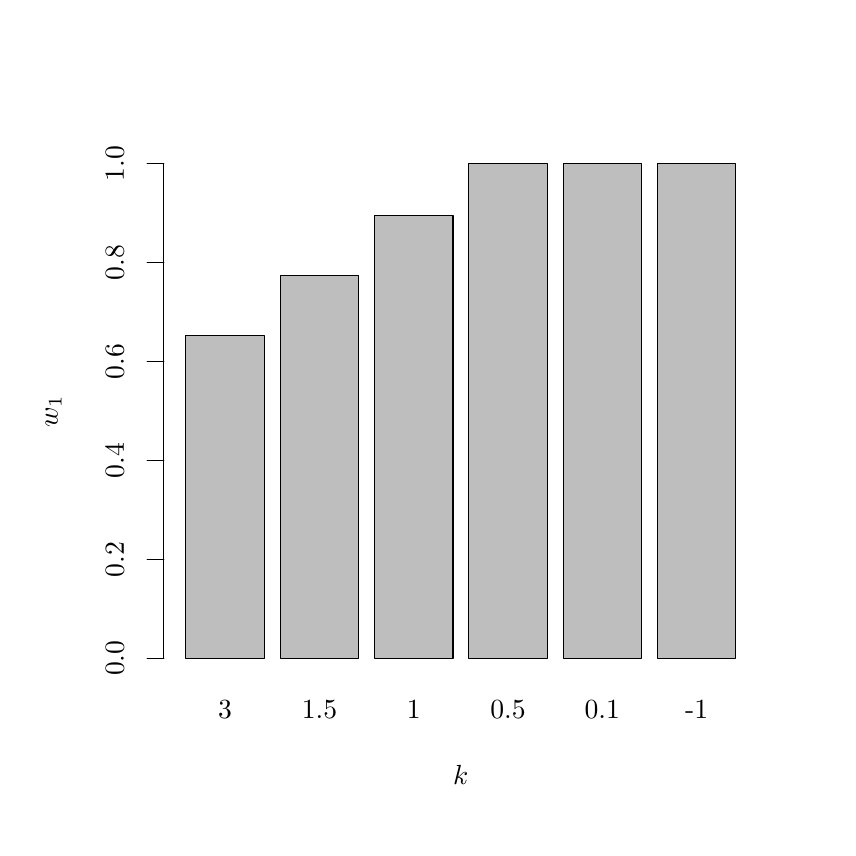
\begin{tikzpicture}[x=1pt,y=1pt]
\definecolor{fillColor}{RGB}{255,255,255}
\path[use as bounding box,fill=fillColor,fill opacity=0.00] (0,0) rectangle (289.08,289.08);
\begin{scope}
\path[clip] (  0.00,  0.00) rectangle (289.08,289.08);
\definecolor{drawColor}{RGB}{0,0,0}
\definecolor{fillColor}{RGB}{190,190,190}

\path[draw=drawColor,line width= 0.4pt,line join=round,line cap=round,fill=fillColor] ( 57.15, 61.20) rectangle ( 85.55,177.81);

\path[draw=drawColor,line width= 0.4pt,line join=round,line cap=round,fill=fillColor] ( 91.23, 61.20) rectangle (119.62,199.53);

\path[draw=drawColor,line width= 0.4pt,line join=round,line cap=round,fill=fillColor] (125.30, 61.20) rectangle (153.70,221.25);

\path[draw=drawColor,line width= 0.4pt,line join=round,line cap=round,fill=fillColor] (159.38, 61.20) rectangle (187.78,239.87);

\path[draw=drawColor,line width= 0.4pt,line join=round,line cap=round,fill=fillColor] (193.46, 61.20) rectangle (221.85,239.87);

\path[draw=drawColor,line width= 0.4pt,line join=round,line cap=round,fill=fillColor] (227.53, 61.20) rectangle (255.93,239.87);
\end{scope}
\begin{scope}
\path[clip] (  0.00,  0.00) rectangle (289.08,289.08);
\definecolor{drawColor}{RGB}{0,0,0}

\node[text=drawColor,anchor=base,inner sep=0pt, outer sep=0pt, scale=  1.00] at ( 71.35, 39.60) {3};

\node[text=drawColor,anchor=base,inner sep=0pt, outer sep=0pt, scale=  1.00] at (105.43, 39.60) {1.5};

\node[text=drawColor,anchor=base,inner sep=0pt, outer sep=0pt, scale=  1.00] at (139.50, 39.60) {1};

\node[text=drawColor,anchor=base,inner sep=0pt, outer sep=0pt, scale=  1.00] at (173.58, 39.60) {0.5};

\node[text=drawColor,anchor=base,inner sep=0pt, outer sep=0pt, scale=  1.00] at (207.65, 39.60) {0.1};

\node[text=drawColor,anchor=base,inner sep=0pt, outer sep=0pt, scale=  1.00] at (241.73, 39.60) {-1};
\end{scope}
\begin{scope}
\path[clip] (  0.00,  0.00) rectangle (289.08,289.08);
\definecolor{drawColor}{RGB}{0,0,0}

\node[text=drawColor,anchor=base,inner sep=0pt, outer sep=0pt, scale=  1.00] at (156.54, 15.60) {$k$};

\node[text=drawColor,rotate= 90.00,anchor=base,inner sep=0pt, outer sep=0pt, scale=  1.00] at ( 10.80,150.54) {$w_1$};
\end{scope}
\begin{scope}
\path[clip] (  0.00,  0.00) rectangle (289.08,289.08);
\definecolor{drawColor}{RGB}{0,0,0}

\path[draw=drawColor,line width= 0.4pt,line join=round,line cap=round] ( 49.20, 61.20) -- ( 49.20,239.88);

\path[draw=drawColor,line width= 0.4pt,line join=round,line cap=round] ( 49.20, 61.20) -- ( 43.20, 61.20);

\path[draw=drawColor,line width= 0.4pt,line join=round,line cap=round] ( 49.20, 96.94) -- ( 43.20, 96.94);

\path[draw=drawColor,line width= 0.4pt,line join=round,line cap=round] ( 49.20,132.67) -- ( 43.20,132.67);

\path[draw=drawColor,line width= 0.4pt,line join=round,line cap=round] ( 49.20,168.41) -- ( 43.20,168.41);

\path[draw=drawColor,line width= 0.4pt,line join=round,line cap=round] ( 49.20,204.14) -- ( 43.20,204.14);

\path[draw=drawColor,line width= 0.4pt,line join=round,line cap=round] ( 49.20,239.88) -- ( 43.20,239.88);

\node[text=drawColor,rotate= 90.00,anchor=base,inner sep=0pt, outer sep=0pt, scale=  1.00] at ( 34.80, 61.20) {0.0};

\node[text=drawColor,rotate= 90.00,anchor=base,inner sep=0pt, outer sep=0pt, scale=  1.00] at ( 34.80, 96.94) {0.2};

\node[text=drawColor,rotate= 90.00,anchor=base,inner sep=0pt, outer sep=0pt, scale=  1.00] at ( 34.80,132.67) {0.4};

\node[text=drawColor,rotate= 90.00,anchor=base,inner sep=0pt, outer sep=0pt, scale=  1.00] at ( 34.80,168.41) {0.6};

\node[text=drawColor,rotate= 90.00,anchor=base,inner sep=0pt, outer sep=0pt, scale=  1.00] at ( 34.80,204.14) {0.8};

\node[text=drawColor,rotate= 90.00,anchor=base,inner sep=0pt, outer sep=0pt, scale=  1.00] at ( 34.80,239.88) {1.0};
\end{scope}
\end{tikzpicture}

	\caption{Plot of the optimized stock weight,
		that is the ratio that should be invested in \texttt{Comp1},
	for different values of $k$. \label{fig:stock_weights}}
\end{figure}

\section{Assignment 2(a)}
\subsection{Problem}
Fit a logistic regression to the data, by numerical maximum likelihood
given parameters $a$ and $b$.
\subsection{Theory and implementation}
There are two reports
$$ \text{reports} = \left\{\underbrace{\text{mature}}_1, \underbrace{\text{immature}}_0\right\} $$
Our model is
$$ y \sim \Bernoulli(f_1(x)), \quad f_1(x) = \frac{\exp\left(a + b (x - 18)\right)}{1 + \exp\left(a + b (x - 18)\right)} $$
$a, b \in \mathbb R$.
The likelihood is given by
$$ \mathcal L(a, b) = \prod_{\text{mature}} f_1(x) \prod_{\text{immature}} f_0(x) $$
\subsection{Results and discussion}
The fitted logistic regression curve is shown in figure~\ref{fig:logistic_regression}.
We see that the result seems plausible since the location where the curve
changes from $0$ to $1$ happens in the middle of the two datasets.

\begin{figure}
	\centering
	% Created by tikzDevice version 0.12.3 on 2019-10-13 21:26:54
% !TEX encoding = UTF-8 Unicode
\begin{tikzpicture}[x=1pt,y=1pt]
\definecolor{fillColor}{RGB}{255,255,255}
\path[use as bounding box,fill=fillColor,fill opacity=0.00] (0,0) rectangle (361.35,361.35);
\begin{scope}
\path[clip] ( 49.20, 61.20) rectangle (336.15,312.15);
\definecolor{drawColor}{RGB}{0,0,0}

\path[draw=drawColor,line width= 0.4pt,line join=round,line cap=round] ( 59.83, 70.49) --
	( 60.36, 70.49) --
	( 60.89, 70.49) --
	( 61.43, 70.49) --
	( 61.96, 70.49) --
	( 62.49, 70.49) --
	( 63.02, 70.49) --
	( 63.55, 70.49) --
	( 64.09, 70.49) --
	( 64.62, 70.49) --
	( 65.15, 70.49) --
	( 65.68, 70.49) --
	( 66.22, 70.49) --
	( 66.75, 70.49) --
	( 67.28, 70.49) --
	( 67.81, 70.49) --
	( 68.35, 70.49) --
	( 68.88, 70.49) --
	( 69.41, 70.49) --
	( 69.94, 70.49) --
	( 70.48, 70.49) --
	( 71.01, 70.49) --
	( 71.54, 70.49) --
	( 72.07, 70.49) --
	( 72.61, 70.49) --
	( 73.14, 70.49) --
	( 73.67, 70.49) --
	( 74.20, 70.49) --
	( 74.74, 70.49) --
	( 75.27, 70.49) --
	( 75.80, 70.49) --
	( 76.33, 70.49) --
	( 76.87, 70.49) --
	( 77.40, 70.49) --
	( 77.93, 70.49) --
	( 78.46, 70.49) --
	( 79.00, 70.49) --
	( 79.53, 70.49) --
	( 80.06, 70.49) --
	( 80.59, 70.49) --
	( 81.13, 70.49) --
	( 81.66, 70.49) --
	( 82.19, 70.49) --
	( 82.72, 70.49) --
	( 83.26, 70.49) --
	( 83.79, 70.49) --
	( 84.32, 70.49) --
	( 84.85, 70.49) --
	( 85.39, 70.49) --
	( 85.92, 70.49) --
	( 86.45, 70.49) --
	( 86.98, 70.49) --
	( 87.52, 70.49) --
	( 88.05, 70.49) --
	( 88.58, 70.49) --
	( 89.11, 70.49) --
	( 89.65, 70.49) --
	( 90.18, 70.49) --
	( 90.71, 70.49) --
	( 91.24, 70.49) --
	( 91.78, 70.49) --
	( 92.31, 70.49) --
	( 92.84, 70.49) --
	( 93.37, 70.49) --
	( 93.90, 70.49) --
	( 94.44, 70.49) --
	( 94.97, 70.49) --
	( 95.50, 70.49) --
	( 96.03, 70.49) --
	( 96.57, 70.49) --
	( 97.10, 70.49) --
	( 97.63, 70.49) --
	( 98.16, 70.49) --
	( 98.70, 70.49) --
	( 99.23, 70.49) --
	( 99.76, 70.49) --
	(100.29, 70.49) --
	(100.83, 70.49) --
	(101.36, 70.49) --
	(101.89, 70.49) --
	(102.42, 70.49) --
	(102.96, 70.49) --
	(103.49, 70.49) --
	(104.02, 70.49) --
	(104.55, 70.49) --
	(105.09, 70.49) --
	(105.62, 70.49) --
	(106.15, 70.49) --
	(106.68, 70.49) --
	(107.22, 70.49) --
	(107.75, 70.49) --
	(108.28, 70.49) --
	(108.81, 70.49) --
	(109.35, 70.49) --
	(109.88, 70.49) --
	(110.41, 70.49) --
	(110.94, 70.49) --
	(111.48, 70.49) --
	(112.01, 70.49) --
	(112.54, 70.49) --
	(113.07, 70.49) --
	(113.61, 70.49) --
	(114.14, 70.49) --
	(114.67, 70.49) --
	(115.20, 70.49) --
	(115.74, 70.49) --
	(116.27, 70.49) --
	(116.80, 70.49) --
	(117.33, 70.49) --
	(117.87, 70.49) --
	(118.40, 70.49) --
	(118.93, 70.49) --
	(119.46, 70.49) --
	(120.00, 70.49) --
	(120.53, 70.49) --
	(121.06, 70.49) --
	(121.59, 70.49) --
	(122.12, 70.49) --
	(122.66, 70.49) --
	(123.19, 70.49) --
	(123.72, 70.49) --
	(124.25, 70.49) --
	(124.79, 70.49) --
	(125.32, 70.49) --
	(125.85, 70.49) --
	(126.38, 70.49) --
	(126.92, 70.50) --
	(127.45, 70.50) --
	(127.98, 70.50) --
	(128.51, 70.50) --
	(129.05, 70.50) --
	(129.58, 70.50) --
	(130.11, 70.50) --
	(130.64, 70.50) --
	(131.18, 70.50) --
	(131.71, 70.50) --
	(132.24, 70.50) --
	(132.77, 70.50) --
	(133.31, 70.50) --
	(133.84, 70.50) --
	(134.37, 70.50) --
	(134.90, 70.50) --
	(135.44, 70.50) --
	(135.97, 70.50) --
	(136.50, 70.50) --
	(137.03, 70.50) --
	(137.57, 70.50) --
	(138.10, 70.50) --
	(138.63, 70.51) --
	(139.16, 70.51) --
	(139.70, 70.51) --
	(140.23, 70.51) --
	(140.76, 70.52) --
	(141.29, 70.52) --
	(141.83, 70.52) --
	(142.36, 70.53) --
	(142.89, 70.53) --
	(143.42, 70.54) --
	(143.96, 70.54) --
	(144.49, 70.55) --
	(145.02, 70.56) --
	(145.55, 70.57) --
	(146.09, 70.58) --
	(146.62, 70.59) --
	(147.15, 70.60) --
	(147.68, 70.62) --
	(148.22, 70.64) --
	(148.75, 70.66) --
	(149.28, 70.68) --
	(149.81, 70.71) --
	(150.34, 70.74) --
	(150.88, 70.78) --
	(151.41, 70.82) --
	(151.94, 70.87) --
	(152.47, 70.92) --
	(153.01, 70.99) --
	(153.54, 71.06) --
	(154.07, 71.14) --
	(154.60, 71.24) --
	(155.14, 71.35) --
	(155.67, 71.48) --
	(156.20, 71.62) --
	(156.73, 71.79) --
	(157.27, 71.97) --
	(157.80, 72.19) --
	(158.33, 72.44) --
	(158.86, 72.73) --
	(159.40, 73.05) --
	(159.93, 73.43) --
	(160.46, 73.86) --
	(160.99, 74.34) --
	(161.53, 74.90) --
	(162.06, 75.54) --
	(162.59, 76.27) --
	(163.12, 77.10) --
	(163.66, 78.05) --
	(164.19, 79.12) --
	(164.72, 80.35) --
	(165.25, 81.73) --
	(165.79, 83.31) --
	(166.32, 85.08) --
	(166.85, 87.09) --
	(167.38, 89.34) --
	(167.92, 91.88) --
	(168.45, 94.71) --
	(168.98, 97.87) --
	(169.51,101.38) --
	(170.05,105.27) --
	(170.58,109.55) --
	(171.11,114.25) --
	(171.64,119.36) --
	(172.18,124.90) --
	(172.71,130.86) --
	(173.24,137.22) --
	(173.77,143.98) --
	(174.31,151.08) --
	(174.84,158.49) --
	(175.37,166.15) --
	(175.90,174.00) --
	(176.44,181.97) --
	(176.97,189.98) --
	(177.50,197.97) --
	(178.03,205.84) --
	(178.56,213.54) --
	(179.10,221.00) --
	(179.63,228.16) --
	(180.16,234.97) --
	(180.69,241.41) --
	(181.23,247.44) --
	(181.76,253.06) --
	(182.29,258.24) --
	(182.82,263.01) --
	(183.36,267.36) --
	(183.89,271.31) --
	(184.42,274.89) --
	(184.95,278.11) --
	(185.49,281.00) --
	(186.02,283.59) --
	(186.55,285.89) --
	(187.08,287.94) --
	(187.62,289.75) --
	(188.15,291.36) --
	(188.68,292.77) --
	(189.21,294.02) --
	(189.75,295.12) --
	(190.28,296.09) --
	(190.81,296.94) --
	(191.34,297.69) --
	(191.88,298.34) --
	(192.41,298.91) --
	(192.94,299.41) --
	(193.47,299.85) --
	(194.01,300.23) --
	(194.54,300.57) --
	(195.07,300.86) --
	(195.60,301.12) --
	(196.14,301.34) --
	(196.67,301.53) --
	(197.20,301.70) --
	(197.73,301.85) --
	(198.27,301.98) --
	(198.80,302.09) --
	(199.33,302.19) --
	(199.86,302.28) --
	(200.40,302.35) --
	(200.93,302.42) --
	(201.46,302.47) --
	(201.99,302.52) --
	(202.53,302.56) --
	(203.06,302.60) --
	(203.59,302.63) --
	(204.12,302.66) --
	(204.66,302.69) --
	(205.19,302.71) --
	(205.72,302.73) --
	(206.25,302.74) --
	(206.79,302.76) --
	(207.32,302.77) --
	(207.85,302.78) --
	(208.38,302.79) --
	(208.91,302.80) --
	(209.45,302.81) --
	(209.98,302.81) --
	(210.51,302.82) --
	(211.04,302.82) --
	(211.58,302.83) --
	(212.11,302.83) --
	(212.64,302.83) --
	(213.17,302.84) --
	(213.71,302.84) --
	(214.24,302.84) --
	(214.77,302.84) --
	(215.30,302.84) --
	(215.84,302.85) --
	(216.37,302.85) --
	(216.90,302.85) --
	(217.43,302.85) --
	(217.97,302.85) --
	(218.50,302.85) --
	(219.03,302.85) --
	(219.56,302.85) --
	(220.10,302.85) --
	(220.63,302.85) --
	(221.16,302.85) --
	(221.69,302.85) --
	(222.23,302.85) --
	(222.76,302.85) --
	(223.29,302.85) --
	(223.82,302.85) --
	(224.36,302.85) --
	(224.89,302.85) --
	(225.42,302.85) --
	(225.95,302.85) --
	(226.49,302.85) --
	(227.02,302.86) --
	(227.55,302.86) --
	(228.08,302.86) --
	(228.62,302.86) --
	(229.15,302.86) --
	(229.68,302.86) --
	(230.21,302.86) --
	(230.75,302.86) --
	(231.28,302.86) --
	(231.81,302.86) --
	(232.34,302.86) --
	(232.88,302.86) --
	(233.41,302.86) --
	(233.94,302.86) --
	(234.47,302.86) --
	(235.01,302.86) --
	(235.54,302.86) --
	(236.07,302.86) --
	(236.60,302.86) --
	(237.13,302.86) --
	(237.67,302.86) --
	(238.20,302.86) --
	(238.73,302.86) --
	(239.26,302.86) --
	(239.80,302.86) --
	(240.33,302.86) --
	(240.86,302.86) --
	(241.39,302.86) --
	(241.93,302.86) --
	(242.46,302.86) --
	(242.99,302.86) --
	(243.52,302.86) --
	(244.06,302.86) --
	(244.59,302.86) --
	(245.12,302.86) --
	(245.65,302.86) --
	(246.19,302.86) --
	(246.72,302.86) --
	(247.25,302.86) --
	(247.78,302.86) --
	(248.32,302.86) --
	(248.85,302.86) --
	(249.38,302.86) --
	(249.91,302.86) --
	(250.45,302.86) --
	(250.98,302.86) --
	(251.51,302.86) --
	(252.04,302.86) --
	(252.58,302.86) --
	(253.11,302.86) --
	(253.64,302.86) --
	(254.17,302.86) --
	(254.71,302.86) --
	(255.24,302.86) --
	(255.77,302.86) --
	(256.30,302.86) --
	(256.84,302.86) --
	(257.37,302.86) --
	(257.90,302.86) --
	(258.43,302.86) --
	(258.97,302.86) --
	(259.50,302.86) --
	(260.03,302.86) --
	(260.56,302.86) --
	(261.10,302.86) --
	(261.63,302.86) --
	(262.16,302.86) --
	(262.69,302.86) --
	(263.23,302.86) --
	(263.76,302.86) --
	(264.29,302.86) --
	(264.82,302.86) --
	(265.35,302.86) --
	(265.89,302.86) --
	(266.42,302.86) --
	(266.95,302.86) --
	(267.48,302.86) --
	(268.02,302.86) --
	(268.55,302.86) --
	(269.08,302.86) --
	(269.61,302.86) --
	(270.15,302.86) --
	(270.68,302.86) --
	(271.21,302.86) --
	(271.74,302.86) --
	(272.28,302.86) --
	(272.81,302.86) --
	(273.34,302.86) --
	(273.87,302.86) --
	(274.41,302.86) --
	(274.94,302.86) --
	(275.47,302.86) --
	(276.00,302.86) --
	(276.54,302.86) --
	(277.07,302.86) --
	(277.60,302.86) --
	(278.13,302.86) --
	(278.67,302.86) --
	(279.20,302.86) --
	(279.73,302.86) --
	(280.26,302.86) --
	(280.80,302.86) --
	(281.33,302.86) --
	(281.86,302.86) --
	(282.39,302.86) --
	(282.93,302.86) --
	(283.46,302.86) --
	(283.99,302.86) --
	(284.52,302.86) --
	(285.06,302.86) --
	(285.59,302.86) --
	(286.12,302.86) --
	(286.65,302.86) --
	(287.19,302.86) --
	(287.72,302.86) --
	(288.25,302.86) --
	(288.78,302.86) --
	(289.32,302.86) --
	(289.85,302.86) --
	(290.38,302.86) --
	(290.91,302.86) --
	(291.45,302.86) --
	(291.98,302.86) --
	(292.51,302.86) --
	(293.04,302.86) --
	(293.57,302.86) --
	(294.11,302.86) --
	(294.64,302.86) --
	(295.17,302.86) --
	(295.70,302.86) --
	(296.24,302.86) --
	(296.77,302.86) --
	(297.30,302.86) --
	(297.83,302.86) --
	(298.37,302.86) --
	(298.90,302.86) --
	(299.43,302.86) --
	(299.96,302.86) --
	(300.50,302.86) --
	(301.03,302.86) --
	(301.56,302.86) --
	(302.09,302.86) --
	(302.63,302.86) --
	(303.16,302.86) --
	(303.69,302.86) --
	(304.22,302.86) --
	(304.76,302.86) --
	(305.29,302.86) --
	(305.82,302.86) --
	(306.35,302.86) --
	(306.89,302.86) --
	(307.42,302.86) --
	(307.95,302.86) --
	(308.48,302.86) --
	(309.02,302.86) --
	(309.55,302.86) --
	(310.08,302.86) --
	(310.61,302.86) --
	(311.15,302.86) --
	(311.68,302.86) --
	(312.21,302.86) --
	(312.74,302.86) --
	(313.28,302.86) --
	(313.81,302.86) --
	(314.34,302.86) --
	(314.87,302.86) --
	(315.41,302.86) --
	(315.94,302.86) --
	(316.47,302.86) --
	(317.00,302.86) --
	(317.54,302.86) --
	(318.07,302.86) --
	(318.60,302.86) --
	(319.13,302.86) --
	(319.67,302.86) --
	(320.20,302.86) --
	(320.73,302.86) --
	(321.26,302.86) --
	(321.80,302.86) --
	(322.33,302.86) --
	(322.86,302.86) --
	(323.39,302.86) --
	(323.92,302.86) --
	(324.46,302.86) --
	(324.99,302.86) --
	(325.52,302.86);
\end{scope}
\begin{scope}
\path[clip] (  0.00,  0.00) rectangle (361.35,361.35);
\definecolor{drawColor}{RGB}{0,0,0}

\path[draw=drawColor,line width= 0.4pt,line join=round,line cap=round] ( 59.83, 61.20) -- (325.52, 61.20);

\path[draw=drawColor,line width= 0.4pt,line join=round,line cap=round] ( 59.83, 61.20) -- ( 59.83, 55.20);

\path[draw=drawColor,line width= 0.4pt,line join=round,line cap=round] (126.25, 61.20) -- (126.25, 55.20);

\path[draw=drawColor,line width= 0.4pt,line join=round,line cap=round] (192.68, 61.20) -- (192.68, 55.20);

\path[draw=drawColor,line width= 0.4pt,line join=round,line cap=round] (259.10, 61.20) -- (259.10, 55.20);

\path[draw=drawColor,line width= 0.4pt,line join=round,line cap=round] (325.52, 61.20) -- (325.52, 55.20);

\node[text=drawColor,anchor=base,inner sep=0pt, outer sep=0pt, scale=  1.00] at ( 59.83, 39.60) {0};

\node[text=drawColor,anchor=base,inner sep=0pt, outer sep=0pt, scale=  1.00] at (126.25, 39.60) {10};

\node[text=drawColor,anchor=base,inner sep=0pt, outer sep=0pt, scale=  1.00] at (192.68, 39.60) {20};

\node[text=drawColor,anchor=base,inner sep=0pt, outer sep=0pt, scale=  1.00] at (259.10, 39.60) {30};

\node[text=drawColor,anchor=base,inner sep=0pt, outer sep=0pt, scale=  1.00] at (325.52, 39.60) {40};

\path[draw=drawColor,line width= 0.4pt,line join=round,line cap=round] ( 49.20, 70.49) -- ( 49.20,302.86);

\path[draw=drawColor,line width= 0.4pt,line join=round,line cap=round] ( 49.20, 70.49) -- ( 43.20, 70.49);

\path[draw=drawColor,line width= 0.4pt,line join=round,line cap=round] ( 49.20,116.97) -- ( 43.20,116.97);

\path[draw=drawColor,line width= 0.4pt,line join=round,line cap=round] ( 49.20,163.44) -- ( 43.20,163.44);

\path[draw=drawColor,line width= 0.4pt,line join=round,line cap=round] ( 49.20,209.91) -- ( 43.20,209.91);

\path[draw=drawColor,line width= 0.4pt,line join=round,line cap=round] ( 49.20,256.38) -- ( 43.20,256.38);

\path[draw=drawColor,line width= 0.4pt,line join=round,line cap=round] ( 49.20,302.86) -- ( 43.20,302.86);

\node[text=drawColor,rotate= 90.00,anchor=base,inner sep=0pt, outer sep=0pt, scale=  1.00] at ( 34.80, 70.49) {0.0};

\node[text=drawColor,rotate= 90.00,anchor=base,inner sep=0pt, outer sep=0pt, scale=  1.00] at ( 34.80,116.97) {0.2};

\node[text=drawColor,rotate= 90.00,anchor=base,inner sep=0pt, outer sep=0pt, scale=  1.00] at ( 34.80,163.44) {0.4};

\node[text=drawColor,rotate= 90.00,anchor=base,inner sep=0pt, outer sep=0pt, scale=  1.00] at ( 34.80,209.91) {0.6};

\node[text=drawColor,rotate= 90.00,anchor=base,inner sep=0pt, outer sep=0pt, scale=  1.00] at ( 34.80,256.38) {0.8};

\node[text=drawColor,rotate= 90.00,anchor=base,inner sep=0pt, outer sep=0pt, scale=  1.00] at ( 34.80,302.86) {1.0};

\path[draw=drawColor,line width= 0.4pt,line join=round,line cap=round] ( 49.20, 61.20) --
	(336.15, 61.20) --
	(336.15,312.15) --
	( 49.20,312.15) --
	( 49.20, 61.20);
\end{scope}
\begin{scope}
\path[clip] (  0.00,  0.00) rectangle (361.35,361.35);
\definecolor{drawColor}{RGB}{0,0,0}

\node[text=drawColor,anchor=base,inner sep=0pt, outer sep=0pt, scale=  1.00] at (192.68, 15.60) {$x$};

\node[text=drawColor,rotate= 90.00,anchor=base,inner sep=0pt, outer sep=0pt, scale=  1.00] at ( 10.80,186.67) {$f_1(x; a, b)$};
\end{scope}
\begin{scope}
\path[clip] ( 49.20, 61.20) rectangle (336.15,312.15);
\definecolor{drawColor}{RGB}{0,0,0}

\path[draw=drawColor,line width= 0.4pt,line join=round,line cap=round] (222.57,302.86) circle (  2.25);

\path[draw=drawColor,line width= 0.4pt,line join=round,line cap=round] (212.60,302.86) circle (  2.25);

\path[draw=drawColor,line width= 0.4pt,line join=round,line cap=round] (203.97,302.86) circle (  2.25);

\path[draw=drawColor,line width= 0.4pt,line join=round,line cap=round] (215.26,302.86) circle (  2.25);

\path[draw=drawColor,line width= 0.4pt,line join=round,line cap=round] (178.73,302.86) circle (  2.25);

\path[draw=drawColor,line width= 0.4pt,line join=round,line cap=round] (212.60,302.86) circle (  2.25);

\path[draw=drawColor,line width= 0.4pt,line join=round,line cap=round] (199.98,302.86) circle (  2.25);

\path[draw=drawColor,line width= 0.4pt,line join=round,line cap=round] (216.59,302.86) circle (  2.25);

\path[draw=drawColor,line width= 0.4pt,line join=round,line cap=round] (186.70,302.86) circle (  2.25);

\path[draw=drawColor,line width= 0.4pt,line join=round,line cap=round] (224.56,302.86) circle (  2.25);

\path[draw=drawColor,line width= 0.4pt,line join=round,line cap=round] (192.01,302.86) circle (  2.25);

\path[draw=drawColor,line width= 0.4pt,line join=round,line cap=round] (189.35,302.86) circle (  2.25);

\path[draw=drawColor,line width= 0.4pt,line join=round,line cap=round] (196.66,302.86) circle (  2.25);

\path[draw=drawColor,line width= 0.4pt,line join=round,line cap=round] (177.40,302.86) circle (  2.25);

\path[draw=drawColor,line width= 0.4pt,line join=round,line cap=round] (213.27,302.86) circle (  2.25);

\path[draw=drawColor,line width= 0.4pt,line join=round,line cap=round] (197.32,302.86) circle (  2.25);

\path[draw=drawColor,line width= 0.4pt,line join=round,line cap=round] (217.92,302.86) circle (  2.25);

\path[draw=drawColor,line width= 0.4pt,line join=round,line cap=round] (220.57,302.86) circle (  2.25);

\path[draw=drawColor,line width= 0.4pt,line join=round,line cap=round] (211.94,302.86) circle (  2.25);

\path[draw=drawColor,line width= 0.4pt,line join=round,line cap=round] (184.70,302.86) circle (  2.25);

\path[draw=drawColor,line width= 0.4pt,line join=round,line cap=round] (217.25,302.86) circle (  2.25);

\path[draw=drawColor,line width= 0.4pt,line join=round,line cap=round] (200.65,302.86) circle (  2.25);

\path[draw=drawColor,line width= 0.4pt,line join=round,line cap=round] (169.43,302.86) circle (  2.25);

\path[draw=drawColor,line width= 0.4pt,line join=round,line cap=round] (214.59,302.86) circle (  2.25);

\path[draw=drawColor,line width= 0.4pt,line join=round,line cap=round] (224.56,302.86) circle (  2.25);

\path[draw=drawColor,line width= 0.4pt,line join=round,line cap=round] (170.76,302.86) circle (  2.25);

\path[draw=drawColor,line width= 0.4pt,line join=round,line cap=round] (178.73,302.86) circle (  2.25);

\path[draw=drawColor,line width= 0.4pt,line join=round,line cap=round] (219.91,302.86) circle (  2.25);

\path[draw=drawColor,line width= 0.4pt,line join=round,line cap=round] (213.93,302.86) circle (  2.25);

\path[draw=drawColor,line width= 0.4pt,line join=round,line cap=round] (214.59,302.86) circle (  2.25);

\path[draw=drawColor,line width= 0.4pt,line join=round,line cap=round] (208.62,302.86) circle (  2.25);

\path[draw=drawColor,line width= 0.4pt,line join=round,line cap=round] (196.66,302.86) circle (  2.25);

\path[draw=drawColor,line width= 0.4pt,line join=round,line cap=round] (174.74,302.86) circle (  2.25);

\path[draw=drawColor,line width= 0.4pt,line join=round,line cap=round] (199.98,302.86) circle (  2.25);

\path[draw=drawColor,line width= 0.4pt,line join=round,line cap=round] (179.39,302.86) circle (  2.25);

\path[draw=drawColor,line width= 0.4pt,line join=round,line cap=round] (193.34,302.86) circle (  2.25);

\path[draw=drawColor,line width= 0.4pt,line join=round,line cap=round] (197.32,302.86) circle (  2.25);

\path[draw=drawColor,line width= 0.4pt,line join=round,line cap=round] (203.97,302.86) circle (  2.25);

\path[draw=drawColor,line width= 0.4pt,line join=round,line cap=round] (206.62,302.86) circle (  2.25);

\path[draw=drawColor,line width= 0.4pt,line join=round,line cap=round] (205.30,302.86) circle (  2.25);

\path[draw=drawColor,line width= 0.4pt,line join=round,line cap=round] (219.91,302.86) circle (  2.25);

\path[draw=drawColor,line width= 0.4pt,line join=round,line cap=round] (203.30,302.86) circle (  2.25);

\path[draw=drawColor,line width= 0.4pt,line join=round,line cap=round] (195.33,302.86) circle (  2.25);

\path[draw=drawColor,line width= 0.4pt,line join=round,line cap=round] (190.02,302.86) circle (  2.25);

\path[draw=drawColor,line width= 0.4pt,line join=round,line cap=round] (185.37,302.86) circle (  2.25);

\path[draw=drawColor,line width= 0.4pt,line join=round,line cap=round] (176.07,302.86) circle (  2.25);

\path[draw=drawColor,line width= 0.4pt,line join=round,line cap=round] (196.66,302.86) circle (  2.25);

\path[draw=drawColor,line width= 0.4pt,line join=round,line cap=round] (188.69,302.86) circle (  2.25);

\path[draw=drawColor,line width= 0.4pt,line join=round,line cap=round] (209.95,302.86) circle (  2.25);

\path[draw=drawColor,line width= 0.4pt,line join=round,line cap=round] (219.91,302.86) circle (  2.25);

\path[draw=drawColor,line width= 0.4pt,line join=round,line cap=round] (147.51, 70.49) circle (  2.25);

\path[draw=drawColor,line width= 0.4pt,line join=round,line cap=round] (158.80, 70.49) circle (  2.25);

\path[draw=drawColor,line width= 0.4pt,line join=round,line cap=round] (157.47, 70.49) circle (  2.25);

\path[draw=drawColor,line width= 0.4pt,line join=round,line cap=round] (148.17, 70.49) circle (  2.25);

\path[draw=drawColor,line width= 0.4pt,line join=round,line cap=round] (176.07, 70.49) circle (  2.25);

\path[draw=drawColor,line width= 0.4pt,line join=round,line cap=round] (152.16, 70.49) circle (  2.25);

\path[draw=drawColor,line width= 0.4pt,line join=round,line cap=round] (166.77, 70.49) circle (  2.25);

\path[draw=drawColor,line width= 0.4pt,line join=round,line cap=round] (152.82, 70.49) circle (  2.25);

\path[draw=drawColor,line width= 0.4pt,line join=round,line cap=round] (152.16, 70.49) circle (  2.25);

\path[draw=drawColor,line width= 0.4pt,line join=round,line cap=round] (153.49, 70.49) circle (  2.25);

\path[draw=drawColor,line width= 0.4pt,line join=round,line cap=round] (158.13, 70.49) circle (  2.25);

\path[draw=drawColor,line width= 0.4pt,line join=round,line cap=round] (160.79, 70.49) circle (  2.25);

\path[draw=drawColor,line width= 0.4pt,line join=round,line cap=round] (144.19, 70.49) circle (  2.25);

\path[draw=drawColor,line width= 0.4pt,line join=round,line cap=round] (157.47, 70.49) circle (  2.25);

\path[draw=drawColor,line width= 0.4pt,line join=round,line cap=round] (168.10, 70.49) circle (  2.25);

\path[draw=drawColor,line width= 0.4pt,line join=round,line cap=round] (140.86, 70.49) circle (  2.25);

\path[draw=drawColor,line width= 0.4pt,line join=round,line cap=round] (142.19, 70.49) circle (  2.25);

\path[draw=drawColor,line width= 0.4pt,line join=round,line cap=round] (157.47, 70.49) circle (  2.25);

\path[draw=drawColor,line width= 0.4pt,line join=round,line cap=round] (164.11, 70.49) circle (  2.25);

\path[draw=drawColor,line width= 0.4pt,line join=round,line cap=round] (156.81, 70.49) circle (  2.25);

\path[draw=drawColor,line width= 0.4pt,line join=round,line cap=round] (158.80, 70.49) circle (  2.25);

\path[draw=drawColor,line width= 0.4pt,line join=round,line cap=round] (172.08, 70.49) circle (  2.25);

\path[draw=drawColor,line width= 0.4pt,line join=round,line cap=round] (171.42, 70.49) circle (  2.25);

\path[draw=drawColor,line width= 0.4pt,line join=round,line cap=round] (164.78, 70.49) circle (  2.25);

\path[draw=drawColor,line width= 0.4pt,line join=round,line cap=round] (163.45, 70.49) circle (  2.25);

\path[draw=drawColor,line width= 0.4pt,line join=round,line cap=round] (167.43, 70.49) circle (  2.25);

\path[draw=drawColor,line width= 0.4pt,line join=round,line cap=round] (170.76, 70.49) circle (  2.25);

\path[draw=drawColor,line width= 0.4pt,line join=round,line cap=round] (140.20, 70.49) circle (  2.25);

\path[draw=drawColor,line width= 0.4pt,line join=round,line cap=round] (170.09, 70.49) circle (  2.25);

\path[draw=drawColor,line width= 0.4pt,line join=round,line cap=round] (157.47, 70.49) circle (  2.25);

\path[draw=drawColor,line width= 0.4pt,line join=round,line cap=round] (156.14, 70.49) circle (  2.25);

\path[draw=drawColor,line width= 0.4pt,line join=round,line cap=round] (166.11, 70.49) circle (  2.25);

\path[draw=drawColor,line width= 0.4pt,line join=round,line cap=round] (186.70, 70.49) circle (  2.25);

\path[draw=drawColor,line width= 0.4pt,line join=round,line cap=round] (151.49, 70.49) circle (  2.25);

\path[draw=drawColor,line width= 0.4pt,line join=round,line cap=round] (144.19, 70.49) circle (  2.25);

\path[draw=drawColor,line width= 0.4pt,line join=round,line cap=round] (178.06, 70.49) circle (  2.25);

\path[draw=drawColor,line width= 0.4pt,line join=round,line cap=round] (172.75, 70.49) circle (  2.25);

\path[draw=drawColor,line width= 0.4pt,line join=round,line cap=round] (158.13, 70.49) circle (  2.25);

\path[draw=drawColor,line width= 0.4pt,line join=round,line cap=round] (160.13, 70.49) circle (  2.25);

\path[draw=drawColor,line width= 0.4pt,line join=round,line cap=round] (141.53, 70.49) circle (  2.25);

\path[draw=drawColor,line width= 0.4pt,line join=round,line cap=round] (159.46, 70.49) circle (  2.25);

\path[draw=drawColor,line width= 0.4pt,line join=round,line cap=round] (164.78, 70.49) circle (  2.25);

\path[draw=drawColor,line width= 0.4pt,line join=round,line cap=round] (173.41, 70.49) circle (  2.25);

\path[draw=drawColor,line width= 0.4pt,line join=round,line cap=round] (141.53, 70.49) circle (  2.25);

\path[draw=drawColor,line width= 0.4pt,line join=round,line cap=round] (171.42, 70.49) circle (  2.25);

\path[draw=drawColor,line width= 0.4pt,line join=round,line cap=round] (143.52, 70.49) circle (  2.25);

\path[draw=drawColor,line width= 0.4pt,line join=round,line cap=round] (148.84, 70.49) circle (  2.25);

\path[draw=drawColor,line width= 0.4pt,line join=round,line cap=round] (163.45, 70.49) circle (  2.25);

\path[draw=drawColor,line width= 0.4pt,line join=round,line cap=round] (170.09, 70.49) circle (  2.25);

\path[draw=drawColor,line width= 0.4pt,line join=round,line cap=round] (178.73, 70.49) circle (  2.25);
\end{scope}
\end{tikzpicture}

	\caption{Plot of the data together with the obtained logistic regression curve. \label{fig:logistic_regression}}
\end{figure}

\section{Assignment 2(b)}
\subsection{Problem}
On a $100 \times 100$ evenly spaced grid of $a$ and $b$ compute and plot
the posterior,
given a uniform prior.
\subsection{Theory and implementation}
Bayes formula for probability mass functions looks like
$$ \pi(x \mid y) = \frac{\pi(y \mid x) \pi(x)}{\pi(y)} $$

The posterior on the grid is visualized with the \texttt{image} R function.
\subsection{Results and discussion}
The posterior on the grid is given in figure~\ref{fig:posterior}.
We see that there is an area, not too small,
where values of $a$ and $b$ are approximately equally likely.
That is to say there exists some uncertainty.

\begin{figure}
	\centering
	% Created by tikzDevice version 0.12.3 on 2019-10-10 21:56:19
% !TEX encoding = UTF-8 Unicode
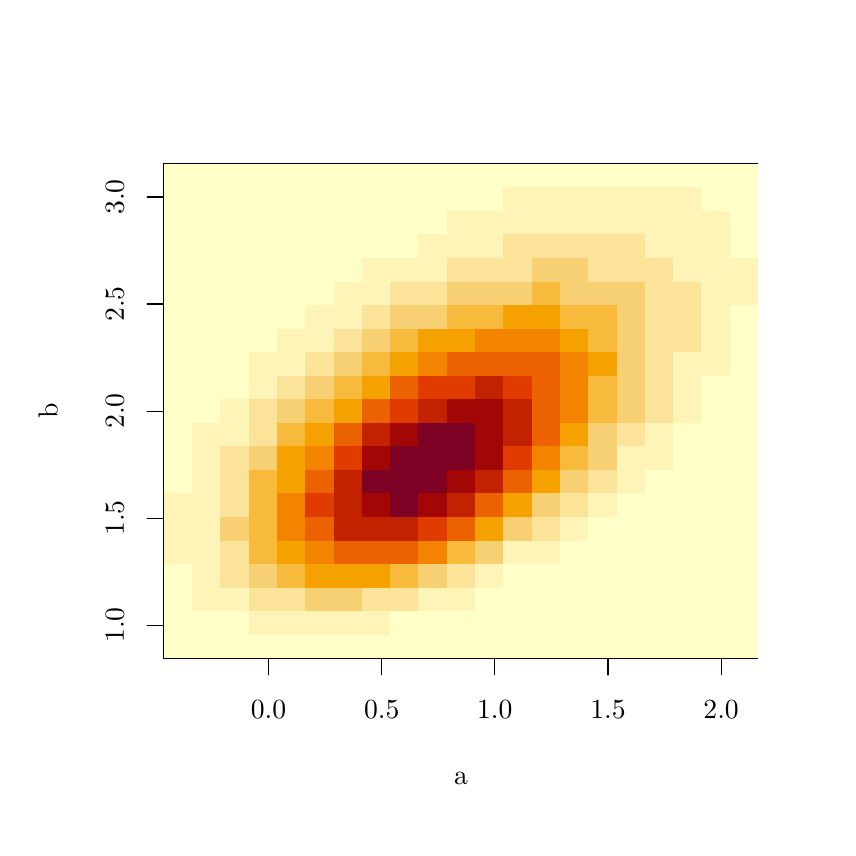
\begin{tikzpicture}[x=1pt,y=1pt]
\definecolor{fillColor}{RGB}{255,255,255}
\path[use as bounding box,fill=fillColor,fill opacity=0.00] (0,0) rectangle (289.08,289.08);
\begin{scope}
\path[clip] (  0.00,  0.00) rectangle (289.08,289.08);
\definecolor{drawColor}{RGB}{0,0,0}

\path[draw=drawColor,line width= 0.4pt,line join=round,line cap=round] ( 87.02, 61.20) -- (250.59, 61.20);

\path[draw=drawColor,line width= 0.4pt,line join=round,line cap=round] ( 87.02, 61.20) -- ( 87.02, 55.20);

\path[draw=drawColor,line width= 0.4pt,line join=round,line cap=round] (127.92, 61.20) -- (127.92, 55.20);

\path[draw=drawColor,line width= 0.4pt,line join=round,line cap=round] (168.81, 61.20) -- (168.81, 55.20);

\path[draw=drawColor,line width= 0.4pt,line join=round,line cap=round] (209.70, 61.20) -- (209.70, 55.20);

\path[draw=drawColor,line width= 0.4pt,line join=round,line cap=round] (250.59, 61.20) -- (250.59, 55.20);

\node[text=drawColor,anchor=base,inner sep=0pt, outer sep=0pt, scale=  1.00] at ( 87.02, 39.60) {0.0};

\node[text=drawColor,anchor=base,inner sep=0pt, outer sep=0pt, scale=  1.00] at (127.92, 39.60) {0.5};

\node[text=drawColor,anchor=base,inner sep=0pt, outer sep=0pt, scale=  1.00] at (168.81, 39.60) {1.0};

\node[text=drawColor,anchor=base,inner sep=0pt, outer sep=0pt, scale=  1.00] at (209.70, 39.60) {1.5};

\node[text=drawColor,anchor=base,inner sep=0pt, outer sep=0pt, scale=  1.00] at (250.59, 39.60) {2.0};

\path[draw=drawColor,line width= 0.4pt,line join=round,line cap=round] ( 49.20, 73.19) -- ( 49.20,227.89);

\path[draw=drawColor,line width= 0.4pt,line join=round,line cap=round] ( 49.20, 73.19) -- ( 43.20, 73.19);

\path[draw=drawColor,line width= 0.4pt,line join=round,line cap=round] ( 49.20,111.86) -- ( 43.20,111.86);

\path[draw=drawColor,line width= 0.4pt,line join=round,line cap=round] ( 49.20,150.54) -- ( 43.20,150.54);

\path[draw=drawColor,line width= 0.4pt,line join=round,line cap=round] ( 49.20,189.22) -- ( 43.20,189.22);

\path[draw=drawColor,line width= 0.4pt,line join=round,line cap=round] ( 49.20,227.89) -- ( 43.20,227.89);

\node[text=drawColor,rotate= 90.00,anchor=base,inner sep=0pt, outer sep=0pt, scale=  1.00] at ( 34.80, 73.19) {1.0};

\node[text=drawColor,rotate= 90.00,anchor=base,inner sep=0pt, outer sep=0pt, scale=  1.00] at ( 34.80,111.86) {1.5};

\node[text=drawColor,rotate= 90.00,anchor=base,inner sep=0pt, outer sep=0pt, scale=  1.00] at ( 34.80,150.54) {2.0};

\node[text=drawColor,rotate= 90.00,anchor=base,inner sep=0pt, outer sep=0pt, scale=  1.00] at ( 34.80,189.22) {2.5};

\node[text=drawColor,rotate= 90.00,anchor=base,inner sep=0pt, outer sep=0pt, scale=  1.00] at ( 34.80,227.89) {3.0};

\path[draw=drawColor,line width= 0.4pt,line join=round,line cap=round] ( 49.20, 61.20) --
	(263.88, 61.20) --
	(263.88,239.88) --
	( 49.20,239.88) --
	( 49.20, 61.20);
\end{scope}
\begin{scope}
\path[clip] (  0.00,  0.00) rectangle (289.08,289.08);
\definecolor{drawColor}{RGB}{0,0,0}

\node[text=drawColor,anchor=base,inner sep=0pt, outer sep=0pt, scale=  1.00] at (156.54, 15.60) {a};

\node[text=drawColor,rotate= 90.00,anchor=base,inner sep=0pt, outer sep=0pt, scale=  1.00] at ( 10.80,150.54) {b};
\end{scope}
\begin{scope}
\path[clip] ( 49.20, 61.20) rectangle (263.88,239.88);
\definecolor{fillColor}{RGB}{255,255,200}

\path[fill=fillColor] ( 49.20, 61.20) rectangle ( 59.42, 69.71);

\path[fill=fillColor] ( 49.20, 69.71) rectangle ( 59.42, 78.22);

\path[fill=fillColor] ( 49.20, 78.22) rectangle ( 59.42, 86.73);

\path[fill=fillColor] ( 49.20, 86.73) rectangle ( 59.42, 95.23);
\definecolor{fillColor}{RGB}{255,244,183}

\path[fill=fillColor] ( 49.20, 95.23) rectangle ( 59.42,103.74);

\path[fill=fillColor] ( 49.20,103.74) rectangle ( 59.42,112.25);

\path[fill=fillColor] ( 49.20,112.25) rectangle ( 59.42,120.76);
\definecolor{fillColor}{RGB}{255,255,200}

\path[fill=fillColor] ( 49.20,120.76) rectangle ( 59.42,129.27);

\path[fill=fillColor] ( 49.20,129.27) rectangle ( 59.42,137.78);

\path[fill=fillColor] ( 49.20,137.78) rectangle ( 59.42,146.29);

\path[fill=fillColor] ( 49.20,146.29) rectangle ( 59.42,154.79);

\path[fill=fillColor] ( 49.20,154.79) rectangle ( 59.42,163.30);

\path[fill=fillColor] ( 49.20,163.30) rectangle ( 59.42,171.81);

\path[fill=fillColor] ( 49.20,171.81) rectangle ( 59.42,180.32);

\path[fill=fillColor] ( 49.20,180.32) rectangle ( 59.42,188.83);

\path[fill=fillColor] ( 49.20,188.83) rectangle ( 59.42,197.34);

\path[fill=fillColor] ( 49.20,197.34) rectangle ( 59.42,205.85);

\path[fill=fillColor] ( 49.20,205.85) rectangle ( 59.42,214.35);

\path[fill=fillColor] ( 49.20,214.35) rectangle ( 59.42,222.86);

\path[fill=fillColor] ( 49.20,222.86) rectangle ( 59.42,231.37);

\path[fill=fillColor] ( 49.20,231.37) rectangle ( 59.42,239.88);

\path[fill=fillColor] ( 59.42, 61.20) rectangle ( 69.65, 69.71);

\path[fill=fillColor] ( 59.42, 69.71) rectangle ( 69.65, 78.22);
\definecolor{fillColor}{RGB}{255,244,183}

\path[fill=fillColor] ( 59.42, 78.22) rectangle ( 69.65, 86.73);

\path[fill=fillColor] ( 59.42, 86.73) rectangle ( 69.65, 95.23);

\path[fill=fillColor] ( 59.42, 95.23) rectangle ( 69.65,103.74);

\path[fill=fillColor] ( 59.42,103.74) rectangle ( 69.65,112.25);

\path[fill=fillColor] ( 59.42,112.25) rectangle ( 69.65,120.76);

\path[fill=fillColor] ( 59.42,120.76) rectangle ( 69.65,129.27);

\path[fill=fillColor] ( 59.42,129.27) rectangle ( 69.65,137.78);

\path[fill=fillColor] ( 59.42,137.78) rectangle ( 69.65,146.29);
\definecolor{fillColor}{RGB}{255,255,200}

\path[fill=fillColor] ( 59.42,146.29) rectangle ( 69.65,154.79);

\path[fill=fillColor] ( 59.42,154.79) rectangle ( 69.65,163.30);

\path[fill=fillColor] ( 59.42,163.30) rectangle ( 69.65,171.81);

\path[fill=fillColor] ( 59.42,171.81) rectangle ( 69.65,180.32);

\path[fill=fillColor] ( 59.42,180.32) rectangle ( 69.65,188.83);

\path[fill=fillColor] ( 59.42,188.83) rectangle ( 69.65,197.34);

\path[fill=fillColor] ( 59.42,197.34) rectangle ( 69.65,205.85);

\path[fill=fillColor] ( 59.42,205.85) rectangle ( 69.65,214.35);

\path[fill=fillColor] ( 59.42,214.35) rectangle ( 69.65,222.86);

\path[fill=fillColor] ( 59.42,222.86) rectangle ( 69.65,231.37);

\path[fill=fillColor] ( 59.42,231.37) rectangle ( 69.65,239.88);

\path[fill=fillColor] ( 69.65, 61.20) rectangle ( 79.87, 69.71);

\path[fill=fillColor] ( 69.65, 69.71) rectangle ( 79.87, 78.22);
\definecolor{fillColor}{RGB}{255,244,183}

\path[fill=fillColor] ( 69.65, 78.22) rectangle ( 79.87, 86.73);
\definecolor{fillColor}{RGB}{251,228,154}

\path[fill=fillColor] ( 69.65, 86.73) rectangle ( 79.87, 95.23);

\path[fill=fillColor] ( 69.65, 95.23) rectangle ( 79.87,103.74);
\definecolor{fillColor}{RGB}{248,208,116}

\path[fill=fillColor] ( 69.65,103.74) rectangle ( 79.87,112.25);
\definecolor{fillColor}{RGB}{251,228,154}

\path[fill=fillColor] ( 69.65,112.25) rectangle ( 79.87,120.76);

\path[fill=fillColor] ( 69.65,120.76) rectangle ( 79.87,129.27);

\path[fill=fillColor] ( 69.65,129.27) rectangle ( 79.87,137.78);
\definecolor{fillColor}{RGB}{255,244,183}

\path[fill=fillColor] ( 69.65,137.78) rectangle ( 79.87,146.29);

\path[fill=fillColor] ( 69.65,146.29) rectangle ( 79.87,154.79);
\definecolor{fillColor}{RGB}{255,255,200}

\path[fill=fillColor] ( 69.65,154.79) rectangle ( 79.87,163.30);

\path[fill=fillColor] ( 69.65,163.30) rectangle ( 79.87,171.81);

\path[fill=fillColor] ( 69.65,171.81) rectangle ( 79.87,180.32);

\path[fill=fillColor] ( 69.65,180.32) rectangle ( 79.87,188.83);

\path[fill=fillColor] ( 69.65,188.83) rectangle ( 79.87,197.34);

\path[fill=fillColor] ( 69.65,197.34) rectangle ( 79.87,205.85);

\path[fill=fillColor] ( 69.65,205.85) rectangle ( 79.87,214.35);

\path[fill=fillColor] ( 69.65,214.35) rectangle ( 79.87,222.86);

\path[fill=fillColor] ( 69.65,222.86) rectangle ( 79.87,231.37);

\path[fill=fillColor] ( 69.65,231.37) rectangle ( 79.87,239.88);

\path[fill=fillColor] ( 79.87, 61.20) rectangle ( 90.09, 69.71);
\definecolor{fillColor}{RGB}{255,244,183}

\path[fill=fillColor] ( 79.87, 69.71) rectangle ( 90.09, 78.22);
\definecolor{fillColor}{RGB}{251,228,154}

\path[fill=fillColor] ( 79.87, 78.22) rectangle ( 90.09, 86.73);
\definecolor{fillColor}{RGB}{248,208,116}

\path[fill=fillColor] ( 79.87, 86.73) rectangle ( 90.09, 95.23);
\definecolor{fillColor}{RGB}{247,186,60}

\path[fill=fillColor] ( 79.87, 95.23) rectangle ( 90.09,103.74);

\path[fill=fillColor] ( 79.87,103.74) rectangle ( 90.09,112.25);

\path[fill=fillColor] ( 79.87,112.25) rectangle ( 90.09,120.76);

\path[fill=fillColor] ( 79.87,120.76) rectangle ( 90.09,129.27);
\definecolor{fillColor}{RGB}{248,208,116}

\path[fill=fillColor] ( 79.87,129.27) rectangle ( 90.09,137.78);
\definecolor{fillColor}{RGB}{251,228,154}

\path[fill=fillColor] ( 79.87,137.78) rectangle ( 90.09,146.29);

\path[fill=fillColor] ( 79.87,146.29) rectangle ( 90.09,154.79);
\definecolor{fillColor}{RGB}{255,244,183}

\path[fill=fillColor] ( 79.87,154.79) rectangle ( 90.09,163.30);

\path[fill=fillColor] ( 79.87,163.30) rectangle ( 90.09,171.81);
\definecolor{fillColor}{RGB}{255,255,200}

\path[fill=fillColor] ( 79.87,171.81) rectangle ( 90.09,180.32);

\path[fill=fillColor] ( 79.87,180.32) rectangle ( 90.09,188.83);

\path[fill=fillColor] ( 79.87,188.83) rectangle ( 90.09,197.34);

\path[fill=fillColor] ( 79.87,197.34) rectangle ( 90.09,205.85);

\path[fill=fillColor] ( 79.87,205.85) rectangle ( 90.09,214.35);

\path[fill=fillColor] ( 79.87,214.35) rectangle ( 90.09,222.86);

\path[fill=fillColor] ( 79.87,222.86) rectangle ( 90.09,231.37);

\path[fill=fillColor] ( 79.87,231.37) rectangle ( 90.09,239.88);

\path[fill=fillColor] ( 90.09, 61.20) rectangle (100.31, 69.71);
\definecolor{fillColor}{RGB}{255,244,183}

\path[fill=fillColor] ( 90.09, 69.71) rectangle (100.31, 78.22);
\definecolor{fillColor}{RGB}{251,228,154}

\path[fill=fillColor] ( 90.09, 78.22) rectangle (100.31, 86.73);
\definecolor{fillColor}{RGB}{247,186,60}

\path[fill=fillColor] ( 90.09, 86.73) rectangle (100.31, 95.23);
\definecolor{fillColor}{RGB}{245,161,0}

\path[fill=fillColor] ( 90.09, 95.23) rectangle (100.31,103.74);
\definecolor{fillColor}{RGB}{242,132,0}

\path[fill=fillColor] ( 90.09,103.74) rectangle (100.31,112.25);

\path[fill=fillColor] ( 90.09,112.25) rectangle (100.31,120.76);
\definecolor{fillColor}{RGB}{245,161,0}

\path[fill=fillColor] ( 90.09,120.76) rectangle (100.31,129.27);

\path[fill=fillColor] ( 90.09,129.27) rectangle (100.31,137.78);
\definecolor{fillColor}{RGB}{247,186,60}

\path[fill=fillColor] ( 90.09,137.78) rectangle (100.31,146.29);
\definecolor{fillColor}{RGB}{248,208,116}

\path[fill=fillColor] ( 90.09,146.29) rectangle (100.31,154.79);
\definecolor{fillColor}{RGB}{251,228,154}

\path[fill=fillColor] ( 90.09,154.79) rectangle (100.31,163.30);
\definecolor{fillColor}{RGB}{255,244,183}

\path[fill=fillColor] ( 90.09,163.30) rectangle (100.31,171.81);

\path[fill=fillColor] ( 90.09,171.81) rectangle (100.31,180.32);
\definecolor{fillColor}{RGB}{255,255,200}

\path[fill=fillColor] ( 90.09,180.32) rectangle (100.31,188.83);

\path[fill=fillColor] ( 90.09,188.83) rectangle (100.31,197.34);

\path[fill=fillColor] ( 90.09,197.34) rectangle (100.31,205.85);

\path[fill=fillColor] ( 90.09,205.85) rectangle (100.31,214.35);

\path[fill=fillColor] ( 90.09,214.35) rectangle (100.31,222.86);

\path[fill=fillColor] ( 90.09,222.86) rectangle (100.31,231.37);

\path[fill=fillColor] ( 90.09,231.37) rectangle (100.31,239.88);

\path[fill=fillColor] (100.31, 61.20) rectangle (110.54, 69.71);
\definecolor{fillColor}{RGB}{255,244,183}

\path[fill=fillColor] (100.31, 69.71) rectangle (110.54, 78.22);
\definecolor{fillColor}{RGB}{248,208,116}

\path[fill=fillColor] (100.31, 78.22) rectangle (110.54, 86.73);
\definecolor{fillColor}{RGB}{245,161,0}

\path[fill=fillColor] (100.31, 86.73) rectangle (110.54, 95.23);
\definecolor{fillColor}{RGB}{242,132,0}

\path[fill=fillColor] (100.31, 95.23) rectangle (110.54,103.74);
\definecolor{fillColor}{RGB}{237,98,0}

\path[fill=fillColor] (100.31,103.74) rectangle (110.54,112.25);
\definecolor{fillColor}{RGB}{225,60,0}

\path[fill=fillColor] (100.31,112.25) rectangle (110.54,120.76);
\definecolor{fillColor}{RGB}{237,98,0}

\path[fill=fillColor] (100.31,120.76) rectangle (110.54,129.27);
\definecolor{fillColor}{RGB}{242,132,0}

\path[fill=fillColor] (100.31,129.27) rectangle (110.54,137.78);
\definecolor{fillColor}{RGB}{245,161,0}

\path[fill=fillColor] (100.31,137.78) rectangle (110.54,146.29);
\definecolor{fillColor}{RGB}{247,186,60}

\path[fill=fillColor] (100.31,146.29) rectangle (110.54,154.79);
\definecolor{fillColor}{RGB}{248,208,116}

\path[fill=fillColor] (100.31,154.79) rectangle (110.54,163.30);
\definecolor{fillColor}{RGB}{251,228,154}

\path[fill=fillColor] (100.31,163.30) rectangle (110.54,171.81);
\definecolor{fillColor}{RGB}{255,244,183}

\path[fill=fillColor] (100.31,171.81) rectangle (110.54,180.32);

\path[fill=fillColor] (100.31,180.32) rectangle (110.54,188.83);
\definecolor{fillColor}{RGB}{255,255,200}

\path[fill=fillColor] (100.31,188.83) rectangle (110.54,197.34);

\path[fill=fillColor] (100.31,197.34) rectangle (110.54,205.85);

\path[fill=fillColor] (100.31,205.85) rectangle (110.54,214.35);

\path[fill=fillColor] (100.31,214.35) rectangle (110.54,222.86);

\path[fill=fillColor] (100.31,222.86) rectangle (110.54,231.37);

\path[fill=fillColor] (100.31,231.37) rectangle (110.54,239.88);

\path[fill=fillColor] (110.54, 61.20) rectangle (120.76, 69.71);
\definecolor{fillColor}{RGB}{255,244,183}

\path[fill=fillColor] (110.54, 69.71) rectangle (120.76, 78.22);
\definecolor{fillColor}{RGB}{248,208,116}

\path[fill=fillColor] (110.54, 78.22) rectangle (120.76, 86.73);
\definecolor{fillColor}{RGB}{245,161,0}

\path[fill=fillColor] (110.54, 86.73) rectangle (120.76, 95.23);
\definecolor{fillColor}{RGB}{237,98,0}

\path[fill=fillColor] (110.54, 95.23) rectangle (120.76,103.74);
\definecolor{fillColor}{RGB}{195,34,0}

\path[fill=fillColor] (110.54,103.74) rectangle (120.76,112.25);

\path[fill=fillColor] (110.54,112.25) rectangle (120.76,120.76);

\path[fill=fillColor] (110.54,120.76) rectangle (120.76,129.27);
\definecolor{fillColor}{RGB}{225,60,0}

\path[fill=fillColor] (110.54,129.27) rectangle (120.76,137.78);
\definecolor{fillColor}{RGB}{237,98,0}

\path[fill=fillColor] (110.54,137.78) rectangle (120.76,146.29);
\definecolor{fillColor}{RGB}{245,161,0}

\path[fill=fillColor] (110.54,146.29) rectangle (120.76,154.79);
\definecolor{fillColor}{RGB}{247,186,60}

\path[fill=fillColor] (110.54,154.79) rectangle (120.76,163.30);
\definecolor{fillColor}{RGB}{248,208,116}

\path[fill=fillColor] (110.54,163.30) rectangle (120.76,171.81);
\definecolor{fillColor}{RGB}{251,228,154}

\path[fill=fillColor] (110.54,171.81) rectangle (120.76,180.32);
\definecolor{fillColor}{RGB}{255,244,183}

\path[fill=fillColor] (110.54,180.32) rectangle (120.76,188.83);

\path[fill=fillColor] (110.54,188.83) rectangle (120.76,197.34);
\definecolor{fillColor}{RGB}{255,255,200}

\path[fill=fillColor] (110.54,197.34) rectangle (120.76,205.85);

\path[fill=fillColor] (110.54,205.85) rectangle (120.76,214.35);

\path[fill=fillColor] (110.54,214.35) rectangle (120.76,222.86);

\path[fill=fillColor] (110.54,222.86) rectangle (120.76,231.37);

\path[fill=fillColor] (110.54,231.37) rectangle (120.76,239.88);

\path[fill=fillColor] (120.76, 61.20) rectangle (130.98, 69.71);
\definecolor{fillColor}{RGB}{255,244,183}

\path[fill=fillColor] (120.76, 69.71) rectangle (130.98, 78.22);
\definecolor{fillColor}{RGB}{251,228,154}

\path[fill=fillColor] (120.76, 78.22) rectangle (130.98, 86.73);
\definecolor{fillColor}{RGB}{245,161,0}

\path[fill=fillColor] (120.76, 86.73) rectangle (130.98, 95.23);
\definecolor{fillColor}{RGB}{237,98,0}

\path[fill=fillColor] (120.76, 95.23) rectangle (130.98,103.74);
\definecolor{fillColor}{RGB}{195,34,0}

\path[fill=fillColor] (120.76,103.74) rectangle (130.98,112.25);
\definecolor{fillColor}{RGB}{162,7,6}

\path[fill=fillColor] (120.76,112.25) rectangle (130.98,120.76);
\definecolor{fillColor}{RGB}{125,0,37}

\path[fill=fillColor] (120.76,120.76) rectangle (130.98,129.27);
\definecolor{fillColor}{RGB}{162,7,6}

\path[fill=fillColor] (120.76,129.27) rectangle (130.98,137.78);
\definecolor{fillColor}{RGB}{195,34,0}

\path[fill=fillColor] (120.76,137.78) rectangle (130.98,146.29);
\definecolor{fillColor}{RGB}{237,98,0}

\path[fill=fillColor] (120.76,146.29) rectangle (130.98,154.79);
\definecolor{fillColor}{RGB}{245,161,0}

\path[fill=fillColor] (120.76,154.79) rectangle (130.98,163.30);
\definecolor{fillColor}{RGB}{247,186,60}

\path[fill=fillColor] (120.76,163.30) rectangle (130.98,171.81);
\definecolor{fillColor}{RGB}{248,208,116}

\path[fill=fillColor] (120.76,171.81) rectangle (130.98,180.32);
\definecolor{fillColor}{RGB}{251,228,154}

\path[fill=fillColor] (120.76,180.32) rectangle (130.98,188.83);
\definecolor{fillColor}{RGB}{255,244,183}

\path[fill=fillColor] (120.76,188.83) rectangle (130.98,197.34);

\path[fill=fillColor] (120.76,197.34) rectangle (130.98,205.85);
\definecolor{fillColor}{RGB}{255,255,200}

\path[fill=fillColor] (120.76,205.85) rectangle (130.98,214.35);

\path[fill=fillColor] (120.76,214.35) rectangle (130.98,222.86);

\path[fill=fillColor] (120.76,222.86) rectangle (130.98,231.37);

\path[fill=fillColor] (120.76,231.37) rectangle (130.98,239.88);

\path[fill=fillColor] (130.98, 61.20) rectangle (141.21, 69.71);

\path[fill=fillColor] (130.98, 69.71) rectangle (141.21, 78.22);
\definecolor{fillColor}{RGB}{251,228,154}

\path[fill=fillColor] (130.98, 78.22) rectangle (141.21, 86.73);
\definecolor{fillColor}{RGB}{247,186,60}

\path[fill=fillColor] (130.98, 86.73) rectangle (141.21, 95.23);
\definecolor{fillColor}{RGB}{237,98,0}

\path[fill=fillColor] (130.98, 95.23) rectangle (141.21,103.74);
\definecolor{fillColor}{RGB}{195,34,0}

\path[fill=fillColor] (130.98,103.74) rectangle (141.21,112.25);
\definecolor{fillColor}{RGB}{125,0,37}

\path[fill=fillColor] (130.98,112.25) rectangle (141.21,120.76);

\path[fill=fillColor] (130.98,120.76) rectangle (141.21,129.27);

\path[fill=fillColor] (130.98,129.27) rectangle (141.21,137.78);
\definecolor{fillColor}{RGB}{162,7,6}

\path[fill=fillColor] (130.98,137.78) rectangle (141.21,146.29);
\definecolor{fillColor}{RGB}{225,60,0}

\path[fill=fillColor] (130.98,146.29) rectangle (141.21,154.79);
\definecolor{fillColor}{RGB}{237,98,0}

\path[fill=fillColor] (130.98,154.79) rectangle (141.21,163.30);
\definecolor{fillColor}{RGB}{245,161,0}

\path[fill=fillColor] (130.98,163.30) rectangle (141.21,171.81);
\definecolor{fillColor}{RGB}{247,186,60}

\path[fill=fillColor] (130.98,171.81) rectangle (141.21,180.32);
\definecolor{fillColor}{RGB}{248,208,116}

\path[fill=fillColor] (130.98,180.32) rectangle (141.21,188.83);
\definecolor{fillColor}{RGB}{251,228,154}

\path[fill=fillColor] (130.98,188.83) rectangle (141.21,197.34);
\definecolor{fillColor}{RGB}{255,244,183}

\path[fill=fillColor] (130.98,197.34) rectangle (141.21,205.85);
\definecolor{fillColor}{RGB}{255,255,200}

\path[fill=fillColor] (130.98,205.85) rectangle (141.21,214.35);

\path[fill=fillColor] (130.98,214.35) rectangle (141.21,222.86);

\path[fill=fillColor] (130.98,222.86) rectangle (141.21,231.37);

\path[fill=fillColor] (130.98,231.37) rectangle (141.21,239.88);

\path[fill=fillColor] (141.21, 61.20) rectangle (151.43, 69.71);

\path[fill=fillColor] (141.21, 69.71) rectangle (151.43, 78.22);
\definecolor{fillColor}{RGB}{255,244,183}

\path[fill=fillColor] (141.21, 78.22) rectangle (151.43, 86.73);
\definecolor{fillColor}{RGB}{248,208,116}

\path[fill=fillColor] (141.21, 86.73) rectangle (151.43, 95.23);
\definecolor{fillColor}{RGB}{242,132,0}

\path[fill=fillColor] (141.21, 95.23) rectangle (151.43,103.74);
\definecolor{fillColor}{RGB}{225,60,0}

\path[fill=fillColor] (141.21,103.74) rectangle (151.43,112.25);
\definecolor{fillColor}{RGB}{162,7,6}

\path[fill=fillColor] (141.21,112.25) rectangle (151.43,120.76);
\definecolor{fillColor}{RGB}{125,0,37}

\path[fill=fillColor] (141.21,120.76) rectangle (151.43,129.27);

\path[fill=fillColor] (141.21,129.27) rectangle (151.43,137.78);

\path[fill=fillColor] (141.21,137.78) rectangle (151.43,146.29);
\definecolor{fillColor}{RGB}{195,34,0}

\path[fill=fillColor] (141.21,146.29) rectangle (151.43,154.79);
\definecolor{fillColor}{RGB}{225,60,0}

\path[fill=fillColor] (141.21,154.79) rectangle (151.43,163.30);
\definecolor{fillColor}{RGB}{242,132,0}

\path[fill=fillColor] (141.21,163.30) rectangle (151.43,171.81);
\definecolor{fillColor}{RGB}{245,161,0}

\path[fill=fillColor] (141.21,171.81) rectangle (151.43,180.32);
\definecolor{fillColor}{RGB}{248,208,116}

\path[fill=fillColor] (141.21,180.32) rectangle (151.43,188.83);
\definecolor{fillColor}{RGB}{251,228,154}

\path[fill=fillColor] (141.21,188.83) rectangle (151.43,197.34);
\definecolor{fillColor}{RGB}{255,244,183}

\path[fill=fillColor] (141.21,197.34) rectangle (151.43,205.85);

\path[fill=fillColor] (141.21,205.85) rectangle (151.43,214.35);
\definecolor{fillColor}{RGB}{255,255,200}

\path[fill=fillColor] (141.21,214.35) rectangle (151.43,222.86);

\path[fill=fillColor] (141.21,222.86) rectangle (151.43,231.37);

\path[fill=fillColor] (141.21,231.37) rectangle (151.43,239.88);

\path[fill=fillColor] (151.43, 61.20) rectangle (161.65, 69.71);

\path[fill=fillColor] (151.43, 69.71) rectangle (161.65, 78.22);
\definecolor{fillColor}{RGB}{255,244,183}

\path[fill=fillColor] (151.43, 78.22) rectangle (161.65, 86.73);
\definecolor{fillColor}{RGB}{251,228,154}

\path[fill=fillColor] (151.43, 86.73) rectangle (161.65, 95.23);
\definecolor{fillColor}{RGB}{247,186,60}

\path[fill=fillColor] (151.43, 95.23) rectangle (161.65,103.74);
\definecolor{fillColor}{RGB}{237,98,0}

\path[fill=fillColor] (151.43,103.74) rectangle (161.65,112.25);
\definecolor{fillColor}{RGB}{195,34,0}

\path[fill=fillColor] (151.43,112.25) rectangle (161.65,120.76);
\definecolor{fillColor}{RGB}{162,7,6}

\path[fill=fillColor] (151.43,120.76) rectangle (161.65,129.27);
\definecolor{fillColor}{RGB}{125,0,37}

\path[fill=fillColor] (151.43,129.27) rectangle (161.65,137.78);

\path[fill=fillColor] (151.43,137.78) rectangle (161.65,146.29);
\definecolor{fillColor}{RGB}{162,7,6}

\path[fill=fillColor] (151.43,146.29) rectangle (161.65,154.79);
\definecolor{fillColor}{RGB}{225,60,0}

\path[fill=fillColor] (151.43,154.79) rectangle (161.65,163.30);
\definecolor{fillColor}{RGB}{237,98,0}

\path[fill=fillColor] (151.43,163.30) rectangle (161.65,171.81);
\definecolor{fillColor}{RGB}{245,161,0}

\path[fill=fillColor] (151.43,171.81) rectangle (161.65,180.32);
\definecolor{fillColor}{RGB}{247,186,60}

\path[fill=fillColor] (151.43,180.32) rectangle (161.65,188.83);
\definecolor{fillColor}{RGB}{248,208,116}

\path[fill=fillColor] (151.43,188.83) rectangle (161.65,197.34);
\definecolor{fillColor}{RGB}{251,228,154}

\path[fill=fillColor] (151.43,197.34) rectangle (161.65,205.85);
\definecolor{fillColor}{RGB}{255,244,183}

\path[fill=fillColor] (151.43,205.85) rectangle (161.65,214.35);

\path[fill=fillColor] (151.43,214.35) rectangle (161.65,222.86);
\definecolor{fillColor}{RGB}{255,255,200}

\path[fill=fillColor] (151.43,222.86) rectangle (161.65,231.37);

\path[fill=fillColor] (151.43,231.37) rectangle (161.65,239.88);

\path[fill=fillColor] (161.65, 61.20) rectangle (171.87, 69.71);

\path[fill=fillColor] (161.65, 69.71) rectangle (171.87, 78.22);

\path[fill=fillColor] (161.65, 78.22) rectangle (171.87, 86.73);
\definecolor{fillColor}{RGB}{255,244,183}

\path[fill=fillColor] (161.65, 86.73) rectangle (171.87, 95.23);
\definecolor{fillColor}{RGB}{248,208,116}

\path[fill=fillColor] (161.65, 95.23) rectangle (171.87,103.74);
\definecolor{fillColor}{RGB}{245,161,0}

\path[fill=fillColor] (161.65,103.74) rectangle (171.87,112.25);
\definecolor{fillColor}{RGB}{237,98,0}

\path[fill=fillColor] (161.65,112.25) rectangle (171.87,120.76);
\definecolor{fillColor}{RGB}{195,34,0}

\path[fill=fillColor] (161.65,120.76) rectangle (171.87,129.27);
\definecolor{fillColor}{RGB}{162,7,6}

\path[fill=fillColor] (161.65,129.27) rectangle (171.87,137.78);

\path[fill=fillColor] (161.65,137.78) rectangle (171.87,146.29);

\path[fill=fillColor] (161.65,146.29) rectangle (171.87,154.79);
\definecolor{fillColor}{RGB}{195,34,0}

\path[fill=fillColor] (161.65,154.79) rectangle (171.87,163.30);
\definecolor{fillColor}{RGB}{237,98,0}

\path[fill=fillColor] (161.65,163.30) rectangle (171.87,171.81);
\definecolor{fillColor}{RGB}{242,132,0}

\path[fill=fillColor] (161.65,171.81) rectangle (171.87,180.32);
\definecolor{fillColor}{RGB}{247,186,60}

\path[fill=fillColor] (161.65,180.32) rectangle (171.87,188.83);
\definecolor{fillColor}{RGB}{248,208,116}

\path[fill=fillColor] (161.65,188.83) rectangle (171.87,197.34);
\definecolor{fillColor}{RGB}{251,228,154}

\path[fill=fillColor] (161.65,197.34) rectangle (171.87,205.85);
\definecolor{fillColor}{RGB}{255,244,183}

\path[fill=fillColor] (161.65,205.85) rectangle (171.87,214.35);

\path[fill=fillColor] (161.65,214.35) rectangle (171.87,222.86);
\definecolor{fillColor}{RGB}{255,255,200}

\path[fill=fillColor] (161.65,222.86) rectangle (171.87,231.37);

\path[fill=fillColor] (161.65,231.37) rectangle (171.87,239.88);

\path[fill=fillColor] (171.87, 61.20) rectangle (182.10, 69.71);

\path[fill=fillColor] (171.87, 69.71) rectangle (182.10, 78.22);

\path[fill=fillColor] (171.87, 78.22) rectangle (182.10, 86.73);

\path[fill=fillColor] (171.87, 86.73) rectangle (182.10, 95.23);
\definecolor{fillColor}{RGB}{255,244,183}

\path[fill=fillColor] (171.87, 95.23) rectangle (182.10,103.74);
\definecolor{fillColor}{RGB}{248,208,116}

\path[fill=fillColor] (171.87,103.74) rectangle (182.10,112.25);
\definecolor{fillColor}{RGB}{245,161,0}

\path[fill=fillColor] (171.87,112.25) rectangle (182.10,120.76);
\definecolor{fillColor}{RGB}{237,98,0}

\path[fill=fillColor] (171.87,120.76) rectangle (182.10,129.27);
\definecolor{fillColor}{RGB}{225,60,0}

\path[fill=fillColor] (171.87,129.27) rectangle (182.10,137.78);
\definecolor{fillColor}{RGB}{195,34,0}

\path[fill=fillColor] (171.87,137.78) rectangle (182.10,146.29);

\path[fill=fillColor] (171.87,146.29) rectangle (182.10,154.79);
\definecolor{fillColor}{RGB}{225,60,0}

\path[fill=fillColor] (171.87,154.79) rectangle (182.10,163.30);
\definecolor{fillColor}{RGB}{237,98,0}

\path[fill=fillColor] (171.87,163.30) rectangle (182.10,171.81);
\definecolor{fillColor}{RGB}{242,132,0}

\path[fill=fillColor] (171.87,171.81) rectangle (182.10,180.32);
\definecolor{fillColor}{RGB}{245,161,0}

\path[fill=fillColor] (171.87,180.32) rectangle (182.10,188.83);
\definecolor{fillColor}{RGB}{248,208,116}

\path[fill=fillColor] (171.87,188.83) rectangle (182.10,197.34);
\definecolor{fillColor}{RGB}{251,228,154}

\path[fill=fillColor] (171.87,197.34) rectangle (182.10,205.85);

\path[fill=fillColor] (171.87,205.85) rectangle (182.10,214.35);
\definecolor{fillColor}{RGB}{255,244,183}

\path[fill=fillColor] (171.87,214.35) rectangle (182.10,222.86);

\path[fill=fillColor] (171.87,222.86) rectangle (182.10,231.37);
\definecolor{fillColor}{RGB}{255,255,200}

\path[fill=fillColor] (171.87,231.37) rectangle (182.10,239.88);

\path[fill=fillColor] (182.10, 61.20) rectangle (192.32, 69.71);

\path[fill=fillColor] (182.10, 69.71) rectangle (192.32, 78.22);

\path[fill=fillColor] (182.10, 78.22) rectangle (192.32, 86.73);

\path[fill=fillColor] (182.10, 86.73) rectangle (192.32, 95.23);
\definecolor{fillColor}{RGB}{255,244,183}

\path[fill=fillColor] (182.10, 95.23) rectangle (192.32,103.74);
\definecolor{fillColor}{RGB}{251,228,154}

\path[fill=fillColor] (182.10,103.74) rectangle (192.32,112.25);
\definecolor{fillColor}{RGB}{248,208,116}

\path[fill=fillColor] (182.10,112.25) rectangle (192.32,120.76);
\definecolor{fillColor}{RGB}{245,161,0}

\path[fill=fillColor] (182.10,120.76) rectangle (192.32,129.27);
\definecolor{fillColor}{RGB}{242,132,0}

\path[fill=fillColor] (182.10,129.27) rectangle (192.32,137.78);
\definecolor{fillColor}{RGB}{237,98,0}

\path[fill=fillColor] (182.10,137.78) rectangle (192.32,146.29);

\path[fill=fillColor] (182.10,146.29) rectangle (192.32,154.79);

\path[fill=fillColor] (182.10,154.79) rectangle (192.32,163.30);

\path[fill=fillColor] (182.10,163.30) rectangle (192.32,171.81);
\definecolor{fillColor}{RGB}{242,132,0}

\path[fill=fillColor] (182.10,171.81) rectangle (192.32,180.32);
\definecolor{fillColor}{RGB}{245,161,0}

\path[fill=fillColor] (182.10,180.32) rectangle (192.32,188.83);
\definecolor{fillColor}{RGB}{247,186,60}

\path[fill=fillColor] (182.10,188.83) rectangle (192.32,197.34);
\definecolor{fillColor}{RGB}{248,208,116}

\path[fill=fillColor] (182.10,197.34) rectangle (192.32,205.85);
\definecolor{fillColor}{RGB}{251,228,154}

\path[fill=fillColor] (182.10,205.85) rectangle (192.32,214.35);
\definecolor{fillColor}{RGB}{255,244,183}

\path[fill=fillColor] (182.10,214.35) rectangle (192.32,222.86);

\path[fill=fillColor] (182.10,222.86) rectangle (192.32,231.37);
\definecolor{fillColor}{RGB}{255,255,200}

\path[fill=fillColor] (182.10,231.37) rectangle (192.32,239.88);

\path[fill=fillColor] (192.32, 61.20) rectangle (202.54, 69.71);

\path[fill=fillColor] (192.32, 69.71) rectangle (202.54, 78.22);

\path[fill=fillColor] (192.32, 78.22) rectangle (202.54, 86.73);

\path[fill=fillColor] (192.32, 86.73) rectangle (202.54, 95.23);

\path[fill=fillColor] (192.32, 95.23) rectangle (202.54,103.74);
\definecolor{fillColor}{RGB}{255,244,183}

\path[fill=fillColor] (192.32,103.74) rectangle (202.54,112.25);
\definecolor{fillColor}{RGB}{251,228,154}

\path[fill=fillColor] (192.32,112.25) rectangle (202.54,120.76);
\definecolor{fillColor}{RGB}{248,208,116}

\path[fill=fillColor] (192.32,120.76) rectangle (202.54,129.27);
\definecolor{fillColor}{RGB}{247,186,60}

\path[fill=fillColor] (192.32,129.27) rectangle (202.54,137.78);
\definecolor{fillColor}{RGB}{245,161,0}

\path[fill=fillColor] (192.32,137.78) rectangle (202.54,146.29);
\definecolor{fillColor}{RGB}{242,132,0}

\path[fill=fillColor] (192.32,146.29) rectangle (202.54,154.79);

\path[fill=fillColor] (192.32,154.79) rectangle (202.54,163.30);

\path[fill=fillColor] (192.32,163.30) rectangle (202.54,171.81);
\definecolor{fillColor}{RGB}{245,161,0}

\path[fill=fillColor] (192.32,171.81) rectangle (202.54,180.32);
\definecolor{fillColor}{RGB}{247,186,60}

\path[fill=fillColor] (192.32,180.32) rectangle (202.54,188.83);
\definecolor{fillColor}{RGB}{248,208,116}

\path[fill=fillColor] (192.32,188.83) rectangle (202.54,197.34);

\path[fill=fillColor] (192.32,197.34) rectangle (202.54,205.85);
\definecolor{fillColor}{RGB}{251,228,154}

\path[fill=fillColor] (192.32,205.85) rectangle (202.54,214.35);
\definecolor{fillColor}{RGB}{255,244,183}

\path[fill=fillColor] (192.32,214.35) rectangle (202.54,222.86);

\path[fill=fillColor] (192.32,222.86) rectangle (202.54,231.37);
\definecolor{fillColor}{RGB}{255,255,200}

\path[fill=fillColor] (192.32,231.37) rectangle (202.54,239.88);

\path[fill=fillColor] (202.54, 61.20) rectangle (212.77, 69.71);

\path[fill=fillColor] (202.54, 69.71) rectangle (212.77, 78.22);

\path[fill=fillColor] (202.54, 78.22) rectangle (212.77, 86.73);

\path[fill=fillColor] (202.54, 86.73) rectangle (212.77, 95.23);

\path[fill=fillColor] (202.54, 95.23) rectangle (212.77,103.74);

\path[fill=fillColor] (202.54,103.74) rectangle (212.77,112.25);
\definecolor{fillColor}{RGB}{255,244,183}

\path[fill=fillColor] (202.54,112.25) rectangle (212.77,120.76);
\definecolor{fillColor}{RGB}{251,228,154}

\path[fill=fillColor] (202.54,120.76) rectangle (212.77,129.27);
\definecolor{fillColor}{RGB}{248,208,116}

\path[fill=fillColor] (202.54,129.27) rectangle (212.77,137.78);

\path[fill=fillColor] (202.54,137.78) rectangle (212.77,146.29);
\definecolor{fillColor}{RGB}{247,186,60}

\path[fill=fillColor] (202.54,146.29) rectangle (212.77,154.79);

\path[fill=fillColor] (202.54,154.79) rectangle (212.77,163.30);
\definecolor{fillColor}{RGB}{245,161,0}

\path[fill=fillColor] (202.54,163.30) rectangle (212.77,171.81);
\definecolor{fillColor}{RGB}{247,186,60}

\path[fill=fillColor] (202.54,171.81) rectangle (212.77,180.32);

\path[fill=fillColor] (202.54,180.32) rectangle (212.77,188.83);
\definecolor{fillColor}{RGB}{248,208,116}

\path[fill=fillColor] (202.54,188.83) rectangle (212.77,197.34);
\definecolor{fillColor}{RGB}{251,228,154}

\path[fill=fillColor] (202.54,197.34) rectangle (212.77,205.85);

\path[fill=fillColor] (202.54,205.85) rectangle (212.77,214.35);
\definecolor{fillColor}{RGB}{255,244,183}

\path[fill=fillColor] (202.54,214.35) rectangle (212.77,222.86);

\path[fill=fillColor] (202.54,222.86) rectangle (212.77,231.37);
\definecolor{fillColor}{RGB}{255,255,200}

\path[fill=fillColor] (202.54,231.37) rectangle (212.77,239.88);

\path[fill=fillColor] (212.77, 61.20) rectangle (222.99, 69.71);

\path[fill=fillColor] (212.77, 69.71) rectangle (222.99, 78.22);

\path[fill=fillColor] (212.77, 78.22) rectangle (222.99, 86.73);

\path[fill=fillColor] (212.77, 86.73) rectangle (222.99, 95.23);

\path[fill=fillColor] (212.77, 95.23) rectangle (222.99,103.74);

\path[fill=fillColor] (212.77,103.74) rectangle (222.99,112.25);

\path[fill=fillColor] (212.77,112.25) rectangle (222.99,120.76);
\definecolor{fillColor}{RGB}{255,244,183}

\path[fill=fillColor] (212.77,120.76) rectangle (222.99,129.27);

\path[fill=fillColor] (212.77,129.27) rectangle (222.99,137.78);
\definecolor{fillColor}{RGB}{251,228,154}

\path[fill=fillColor] (212.77,137.78) rectangle (222.99,146.29);
\definecolor{fillColor}{RGB}{248,208,116}

\path[fill=fillColor] (212.77,146.29) rectangle (222.99,154.79);

\path[fill=fillColor] (212.77,154.79) rectangle (222.99,163.30);

\path[fill=fillColor] (212.77,163.30) rectangle (222.99,171.81);

\path[fill=fillColor] (212.77,171.81) rectangle (222.99,180.32);

\path[fill=fillColor] (212.77,180.32) rectangle (222.99,188.83);

\path[fill=fillColor] (212.77,188.83) rectangle (222.99,197.34);
\definecolor{fillColor}{RGB}{251,228,154}

\path[fill=fillColor] (212.77,197.34) rectangle (222.99,205.85);

\path[fill=fillColor] (212.77,205.85) rectangle (222.99,214.35);
\definecolor{fillColor}{RGB}{255,244,183}

\path[fill=fillColor] (212.77,214.35) rectangle (222.99,222.86);

\path[fill=fillColor] (212.77,222.86) rectangle (222.99,231.37);
\definecolor{fillColor}{RGB}{255,255,200}

\path[fill=fillColor] (212.77,231.37) rectangle (222.99,239.88);

\path[fill=fillColor] (222.99, 61.20) rectangle (233.21, 69.71);

\path[fill=fillColor] (222.99, 69.71) rectangle (233.21, 78.22);

\path[fill=fillColor] (222.99, 78.22) rectangle (233.21, 86.73);

\path[fill=fillColor] (222.99, 86.73) rectangle (233.21, 95.23);

\path[fill=fillColor] (222.99, 95.23) rectangle (233.21,103.74);

\path[fill=fillColor] (222.99,103.74) rectangle (233.21,112.25);

\path[fill=fillColor] (222.99,112.25) rectangle (233.21,120.76);

\path[fill=fillColor] (222.99,120.76) rectangle (233.21,129.27);
\definecolor{fillColor}{RGB}{255,244,183}

\path[fill=fillColor] (222.99,129.27) rectangle (233.21,137.78);

\path[fill=fillColor] (222.99,137.78) rectangle (233.21,146.29);
\definecolor{fillColor}{RGB}{251,228,154}

\path[fill=fillColor] (222.99,146.29) rectangle (233.21,154.79);

\path[fill=fillColor] (222.99,154.79) rectangle (233.21,163.30);

\path[fill=fillColor] (222.99,163.30) rectangle (233.21,171.81);

\path[fill=fillColor] (222.99,171.81) rectangle (233.21,180.32);

\path[fill=fillColor] (222.99,180.32) rectangle (233.21,188.83);

\path[fill=fillColor] (222.99,188.83) rectangle (233.21,197.34);

\path[fill=fillColor] (222.99,197.34) rectangle (233.21,205.85);
\definecolor{fillColor}{RGB}{255,244,183}

\path[fill=fillColor] (222.99,205.85) rectangle (233.21,214.35);

\path[fill=fillColor] (222.99,214.35) rectangle (233.21,222.86);

\path[fill=fillColor] (222.99,222.86) rectangle (233.21,231.37);
\definecolor{fillColor}{RGB}{255,255,200}

\path[fill=fillColor] (222.99,231.37) rectangle (233.21,239.88);

\path[fill=fillColor] (233.21, 61.20) rectangle (243.43, 69.71);

\path[fill=fillColor] (233.21, 69.71) rectangle (243.43, 78.22);

\path[fill=fillColor] (233.21, 78.22) rectangle (243.43, 86.73);

\path[fill=fillColor] (233.21, 86.73) rectangle (243.43, 95.23);

\path[fill=fillColor] (233.21, 95.23) rectangle (243.43,103.74);

\path[fill=fillColor] (233.21,103.74) rectangle (243.43,112.25);

\path[fill=fillColor] (233.21,112.25) rectangle (243.43,120.76);

\path[fill=fillColor] (233.21,120.76) rectangle (243.43,129.27);

\path[fill=fillColor] (233.21,129.27) rectangle (243.43,137.78);

\path[fill=fillColor] (233.21,137.78) rectangle (243.43,146.29);
\definecolor{fillColor}{RGB}{255,244,183}

\path[fill=fillColor] (233.21,146.29) rectangle (243.43,154.79);

\path[fill=fillColor] (233.21,154.79) rectangle (243.43,163.30);

\path[fill=fillColor] (233.21,163.30) rectangle (243.43,171.81);
\definecolor{fillColor}{RGB}{251,228,154}

\path[fill=fillColor] (233.21,171.81) rectangle (243.43,180.32);

\path[fill=fillColor] (233.21,180.32) rectangle (243.43,188.83);

\path[fill=fillColor] (233.21,188.83) rectangle (243.43,197.34);
\definecolor{fillColor}{RGB}{255,244,183}

\path[fill=fillColor] (233.21,197.34) rectangle (243.43,205.85);

\path[fill=fillColor] (233.21,205.85) rectangle (243.43,214.35);

\path[fill=fillColor] (233.21,214.35) rectangle (243.43,222.86);

\path[fill=fillColor] (233.21,222.86) rectangle (243.43,231.37);
\definecolor{fillColor}{RGB}{255,255,200}

\path[fill=fillColor] (233.21,231.37) rectangle (243.43,239.88);

\path[fill=fillColor] (243.43, 61.20) rectangle (253.66, 69.71);

\path[fill=fillColor] (243.43, 69.71) rectangle (253.66, 78.22);

\path[fill=fillColor] (243.43, 78.22) rectangle (253.66, 86.73);

\path[fill=fillColor] (243.43, 86.73) rectangle (253.66, 95.23);

\path[fill=fillColor] (243.43, 95.23) rectangle (253.66,103.74);

\path[fill=fillColor] (243.43,103.74) rectangle (253.66,112.25);

\path[fill=fillColor] (243.43,112.25) rectangle (253.66,120.76);

\path[fill=fillColor] (243.43,120.76) rectangle (253.66,129.27);

\path[fill=fillColor] (243.43,129.27) rectangle (253.66,137.78);

\path[fill=fillColor] (243.43,137.78) rectangle (253.66,146.29);

\path[fill=fillColor] (243.43,146.29) rectangle (253.66,154.79);

\path[fill=fillColor] (243.43,154.79) rectangle (253.66,163.30);
\definecolor{fillColor}{RGB}{255,244,183}

\path[fill=fillColor] (243.43,163.30) rectangle (253.66,171.81);

\path[fill=fillColor] (243.43,171.81) rectangle (253.66,180.32);

\path[fill=fillColor] (243.43,180.32) rectangle (253.66,188.83);

\path[fill=fillColor] (243.43,188.83) rectangle (253.66,197.34);

\path[fill=fillColor] (243.43,197.34) rectangle (253.66,205.85);

\path[fill=fillColor] (243.43,205.85) rectangle (253.66,214.35);

\path[fill=fillColor] (243.43,214.35) rectangle (253.66,222.86);
\definecolor{fillColor}{RGB}{255,255,200}

\path[fill=fillColor] (243.43,222.86) rectangle (253.66,231.37);

\path[fill=fillColor] (243.43,231.37) rectangle (253.66,239.88);

\path[fill=fillColor] (253.66, 61.20) rectangle (263.88, 69.71);

\path[fill=fillColor] (253.66, 69.71) rectangle (263.88, 78.22);

\path[fill=fillColor] (253.66, 78.22) rectangle (263.88, 86.73);

\path[fill=fillColor] (253.66, 86.73) rectangle (263.88, 95.23);

\path[fill=fillColor] (253.66, 95.23) rectangle (263.88,103.74);

\path[fill=fillColor] (253.66,103.74) rectangle (263.88,112.25);

\path[fill=fillColor] (253.66,112.25) rectangle (263.88,120.76);

\path[fill=fillColor] (253.66,120.76) rectangle (263.88,129.27);

\path[fill=fillColor] (253.66,129.27) rectangle (263.88,137.78);

\path[fill=fillColor] (253.66,137.78) rectangle (263.88,146.29);

\path[fill=fillColor] (253.66,146.29) rectangle (263.88,154.79);

\path[fill=fillColor] (253.66,154.79) rectangle (263.88,163.30);

\path[fill=fillColor] (253.66,163.30) rectangle (263.88,171.81);

\path[fill=fillColor] (253.66,171.81) rectangle (263.88,180.32);

\path[fill=fillColor] (253.66,180.32) rectangle (263.88,188.83);
\definecolor{fillColor}{RGB}{255,244,183}

\path[fill=fillColor] (253.66,188.83) rectangle (263.88,197.34);

\path[fill=fillColor] (253.66,197.34) rectangle (263.88,205.85);
\definecolor{fillColor}{RGB}{255,255,200}

\path[fill=fillColor] (253.66,205.85) rectangle (263.88,214.35);

\path[fill=fillColor] (253.66,214.35) rectangle (263.88,222.86);

\path[fill=fillColor] (253.66,222.86) rectangle (263.88,231.37);

\path[fill=fillColor] (253.66,231.37) rectangle (263.88,239.88);
\end{scope}
\end{tikzpicture}

	\caption{The posterior on the $a, b$ grid from $-0.4, 0.9$ to $2.1, 3.1$.
		The whiter areas contain smaller densities, while the redder contain larger.
	\label{fig:posterior}}
\end{figure}

\section{Assignment 2(c)}\label{sec:optimal_decision}
\subsection{Problem}
With the ML estimates of $a$ and $b$,
for each cost function, $c_1$; $c_2$,
find $\gamma$ and $\alpha$ in the distribution of true ages so that
the optimal decision is to classify those with mature knees as adults.
\subsection{Theory and implementation}
Given $\alpha, \mu > 0$ the true age probablity density is assumed to be given by
$$ \pi(x; \mu, \alpha) = \begin{cases}
	0, & x < 14 \\
	\GammaD(x - 14; \alpha, \alpha / (\mu - 14)), & x \ge 14
\end{cases} $$
The two cost functions in question are defined as
$$ c_1(x) = \begin{cases} B, & x \le 18 \\ 1, & x > 18 \end{cases}
\quad \text{and} \quad
c_2(x) = \begin{cases} B (18 - x), & x \le 18 \\ x - 18, & x > 18 \end{cases} $$
where $B$ is fixed to $B = 10$.
They represent the cost of misclassifying someone whose true age is $x$ years.
Now
\begin{equation}\label{eq:costs}
C_c = \int_{18}^\infty \pi(x; \mu, \alpha) f_k(x) c(x) \, dx, \quad C_a = \int_0^{18} \pi(x; \mu, \alpha) f_k(x) c(x) \, dx
\end{equation}
give the expected cost of misclassification
if one classifies as child or adult respectively.
Therefore if $C_c < C_a$ on should classify as children, otherwise as adults.

The optimal decision is queried over a grid of reasonable $\mu$ and $\alpha$ values
from $15, 2$ to $25, 9$ and the result is visualized.
\subsection{Results and discussion}
The optimal decision over the grid is shown in figure~\ref{fig:optimal_decision}.

\begin{figure}
	\centering
	\begin{subfigure}[b]{0.4\textwidth}
		% Created by tikzDevice version 0.12.3 on 2019-10-13 22:11:50
% !TEX encoding = UTF-8 Unicode
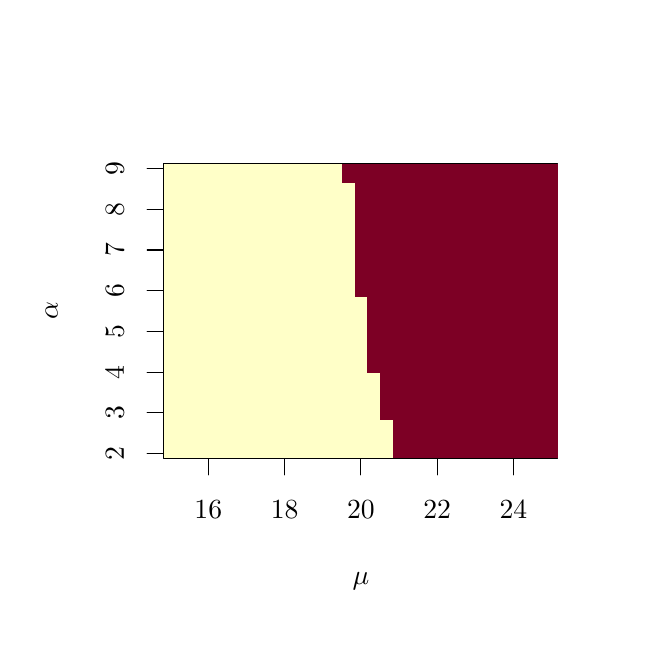
\begin{tikzpicture}[x=1pt,y=1pt]
\definecolor{fillColor}{RGB}{255,255,255}
\path[use as bounding box,fill=fillColor,fill opacity=0.00] (0,0) rectangle (216.81,216.81);
\begin{scope}
\path[clip] (  0.00,  0.00) rectangle (216.81,216.81);
\definecolor{drawColor}{RGB}{0,0,0}

\path[draw=drawColor,line width= 0.4pt,line join=round,line cap=round] ( 65.28, 61.20) -- (175.53, 61.20);

\path[draw=drawColor,line width= 0.4pt,line join=round,line cap=round] ( 65.28, 61.20) -- ( 65.28, 55.20);

\path[draw=drawColor,line width= 0.4pt,line join=round,line cap=round] ( 92.84, 61.20) -- ( 92.84, 55.20);

\path[draw=drawColor,line width= 0.4pt,line join=round,line cap=round] (120.40, 61.20) -- (120.40, 55.20);

\path[draw=drawColor,line width= 0.4pt,line join=round,line cap=round] (147.97, 61.20) -- (147.97, 55.20);

\path[draw=drawColor,line width= 0.4pt,line join=round,line cap=round] (175.53, 61.20) -- (175.53, 55.20);

\node[text=drawColor,anchor=base,inner sep=0pt, outer sep=0pt, scale=  1.00] at ( 65.28, 39.60) {16};

\node[text=drawColor,anchor=base,inner sep=0pt, outer sep=0pt, scale=  1.00] at ( 92.84, 39.60) {18};

\node[text=drawColor,anchor=base,inner sep=0pt, outer sep=0pt, scale=  1.00] at (120.40, 39.60) {20};

\node[text=drawColor,anchor=base,inner sep=0pt, outer sep=0pt, scale=  1.00] at (147.97, 39.60) {22};

\node[text=drawColor,anchor=base,inner sep=0pt, outer sep=0pt, scale=  1.00] at (175.53, 39.60) {24};

\path[draw=drawColor,line width= 0.4pt,line join=round,line cap=round] ( 49.20, 62.92) -- ( 49.20,165.89);

\path[draw=drawColor,line width= 0.4pt,line join=round,line cap=round] ( 49.20, 62.92) -- ( 43.20, 62.92);

\path[draw=drawColor,line width= 0.4pt,line join=round,line cap=round] ( 49.20, 77.63) -- ( 43.20, 77.63);

\path[draw=drawColor,line width= 0.4pt,line join=round,line cap=round] ( 49.20, 92.34) -- ( 43.20, 92.34);

\path[draw=drawColor,line width= 0.4pt,line join=round,line cap=round] ( 49.20,107.05) -- ( 43.20,107.05);

\path[draw=drawColor,line width= 0.4pt,line join=round,line cap=round] ( 49.20,121.76) -- ( 43.20,121.76);

\path[draw=drawColor,line width= 0.4pt,line join=round,line cap=round] ( 49.20,136.47) -- ( 43.20,136.47);

\path[draw=drawColor,line width= 0.4pt,line join=round,line cap=round] ( 49.20,151.18) -- ( 43.20,151.18);

\path[draw=drawColor,line width= 0.4pt,line join=round,line cap=round] ( 49.20,165.89) -- ( 43.20,165.89);

\node[text=drawColor,rotate= 90.00,anchor=base,inner sep=0pt, outer sep=0pt, scale=  1.00] at ( 34.80, 62.92) {2};

\node[text=drawColor,rotate= 90.00,anchor=base,inner sep=0pt, outer sep=0pt, scale=  1.00] at ( 34.80, 77.63) {3};

\node[text=drawColor,rotate= 90.00,anchor=base,inner sep=0pt, outer sep=0pt, scale=  1.00] at ( 34.80, 92.34) {4};

\node[text=drawColor,rotate= 90.00,anchor=base,inner sep=0pt, outer sep=0pt, scale=  1.00] at ( 34.80,107.05) {5};

\node[text=drawColor,rotate= 90.00,anchor=base,inner sep=0pt, outer sep=0pt, scale=  1.00] at ( 34.80,121.76) {6};

\node[text=drawColor,rotate= 90.00,anchor=base,inner sep=0pt, outer sep=0pt, scale=  1.00] at ( 34.80,136.47) {7};

\node[text=drawColor,rotate= 90.00,anchor=base,inner sep=0pt, outer sep=0pt, scale=  1.00] at ( 34.80,151.18) {8};

\node[text=drawColor,rotate= 90.00,anchor=base,inner sep=0pt, outer sep=0pt, scale=  1.00] at ( 34.80,165.89) {9};

\path[draw=drawColor,line width= 0.4pt,line join=round,line cap=round] ( 49.20, 61.20) --
	(191.61, 61.20) --
	(191.61,167.61) --
	( 49.20,167.61) --
	( 49.20, 61.20);
\end{scope}
\begin{scope}
\path[clip] (  0.00,  0.00) rectangle (216.81,216.81);
\definecolor{drawColor}{RGB}{0,0,0}

\node[text=drawColor,anchor=base,inner sep=0pt, outer sep=0pt, scale=  1.00] at (120.40, 15.60) {$\mu$};

\node[text=drawColor,rotate= 90.00,anchor=base,inner sep=0pt, outer sep=0pt, scale=  1.00] at ( 10.80,114.41) {$\alpha$};
\end{scope}
\begin{scope}
\path[clip] ( 49.20, 61.20) rectangle (191.61,167.61);
\definecolor{fillColor}{RGB}{255,255,200}

\path[fill=fillColor] ( 49.20, 61.20) rectangle ( 53.79, 64.63);

\path[fill=fillColor] ( 49.20, 64.63) rectangle ( 53.79, 68.07);

\path[fill=fillColor] ( 49.20, 68.07) rectangle ( 53.79, 71.50);

\path[fill=fillColor] ( 49.20, 71.50) rectangle ( 53.79, 74.93);

\path[fill=fillColor] ( 49.20, 74.93) rectangle ( 53.79, 78.36);

\path[fill=fillColor] ( 49.20, 78.36) rectangle ( 53.79, 81.80);

\path[fill=fillColor] ( 49.20, 81.80) rectangle ( 53.79, 85.23);

\path[fill=fillColor] ( 49.20, 85.23) rectangle ( 53.79, 88.66);

\path[fill=fillColor] ( 49.20, 88.66) rectangle ( 53.79, 92.09);

\path[fill=fillColor] ( 49.20, 92.09) rectangle ( 53.79, 95.53);

\path[fill=fillColor] ( 49.20, 95.53) rectangle ( 53.79, 98.96);

\path[fill=fillColor] ( 49.20, 98.96) rectangle ( 53.79,102.39);

\path[fill=fillColor] ( 49.20,102.39) rectangle ( 53.79,105.82);

\path[fill=fillColor] ( 49.20,105.82) rectangle ( 53.79,109.26);

\path[fill=fillColor] ( 49.20,109.26) rectangle ( 53.79,112.69);

\path[fill=fillColor] ( 49.20,112.69) rectangle ( 53.79,116.12);

\path[fill=fillColor] ( 49.20,116.12) rectangle ( 53.79,119.55);

\path[fill=fillColor] ( 49.20,119.55) rectangle ( 53.79,122.99);

\path[fill=fillColor] ( 49.20,122.99) rectangle ( 53.79,126.42);

\path[fill=fillColor] ( 49.20,126.42) rectangle ( 53.79,129.85);

\path[fill=fillColor] ( 49.20,129.85) rectangle ( 53.79,133.28);

\path[fill=fillColor] ( 49.20,133.28) rectangle ( 53.79,136.72);

\path[fill=fillColor] ( 49.20,136.72) rectangle ( 53.79,140.15);

\path[fill=fillColor] ( 49.20,140.15) rectangle ( 53.79,143.58);

\path[fill=fillColor] ( 49.20,143.58) rectangle ( 53.79,147.01);

\path[fill=fillColor] ( 49.20,147.01) rectangle ( 53.79,150.45);

\path[fill=fillColor] ( 49.20,150.45) rectangle ( 53.79,153.88);

\path[fill=fillColor] ( 49.20,153.88) rectangle ( 53.79,157.31);

\path[fill=fillColor] ( 49.20,157.31) rectangle ( 53.79,160.74);

\path[fill=fillColor] ( 49.20,160.74) rectangle ( 53.79,164.18);

\path[fill=fillColor] ( 49.20,164.18) rectangle ( 53.79,167.61);

\path[fill=fillColor] ( 53.79, 61.20) rectangle ( 58.39, 64.63);

\path[fill=fillColor] ( 53.79, 64.63) rectangle ( 58.39, 68.07);

\path[fill=fillColor] ( 53.79, 68.07) rectangle ( 58.39, 71.50);

\path[fill=fillColor] ( 53.79, 71.50) rectangle ( 58.39, 74.93);

\path[fill=fillColor] ( 53.79, 74.93) rectangle ( 58.39, 78.36);

\path[fill=fillColor] ( 53.79, 78.36) rectangle ( 58.39, 81.80);

\path[fill=fillColor] ( 53.79, 81.80) rectangle ( 58.39, 85.23);

\path[fill=fillColor] ( 53.79, 85.23) rectangle ( 58.39, 88.66);

\path[fill=fillColor] ( 53.79, 88.66) rectangle ( 58.39, 92.09);

\path[fill=fillColor] ( 53.79, 92.09) rectangle ( 58.39, 95.53);

\path[fill=fillColor] ( 53.79, 95.53) rectangle ( 58.39, 98.96);

\path[fill=fillColor] ( 53.79, 98.96) rectangle ( 58.39,102.39);

\path[fill=fillColor] ( 53.79,102.39) rectangle ( 58.39,105.82);

\path[fill=fillColor] ( 53.79,105.82) rectangle ( 58.39,109.26);

\path[fill=fillColor] ( 53.79,109.26) rectangle ( 58.39,112.69);

\path[fill=fillColor] ( 53.79,112.69) rectangle ( 58.39,116.12);

\path[fill=fillColor] ( 53.79,116.12) rectangle ( 58.39,119.55);

\path[fill=fillColor] ( 53.79,119.55) rectangle ( 58.39,122.99);

\path[fill=fillColor] ( 53.79,122.99) rectangle ( 58.39,126.42);

\path[fill=fillColor] ( 53.79,126.42) rectangle ( 58.39,129.85);

\path[fill=fillColor] ( 53.79,129.85) rectangle ( 58.39,133.28);

\path[fill=fillColor] ( 53.79,133.28) rectangle ( 58.39,136.72);

\path[fill=fillColor] ( 53.79,136.72) rectangle ( 58.39,140.15);

\path[fill=fillColor] ( 53.79,140.15) rectangle ( 58.39,143.58);

\path[fill=fillColor] ( 53.79,143.58) rectangle ( 58.39,147.01);

\path[fill=fillColor] ( 53.79,147.01) rectangle ( 58.39,150.45);

\path[fill=fillColor] ( 53.79,150.45) rectangle ( 58.39,153.88);

\path[fill=fillColor] ( 53.79,153.88) rectangle ( 58.39,157.31);

\path[fill=fillColor] ( 53.79,157.31) rectangle ( 58.39,160.74);

\path[fill=fillColor] ( 53.79,160.74) rectangle ( 58.39,164.18);

\path[fill=fillColor] ( 53.79,164.18) rectangle ( 58.39,167.61);

\path[fill=fillColor] ( 58.39, 61.20) rectangle ( 62.98, 64.63);

\path[fill=fillColor] ( 58.39, 64.63) rectangle ( 62.98, 68.07);

\path[fill=fillColor] ( 58.39, 68.07) rectangle ( 62.98, 71.50);

\path[fill=fillColor] ( 58.39, 71.50) rectangle ( 62.98, 74.93);

\path[fill=fillColor] ( 58.39, 74.93) rectangle ( 62.98, 78.36);

\path[fill=fillColor] ( 58.39, 78.36) rectangle ( 62.98, 81.80);

\path[fill=fillColor] ( 58.39, 81.80) rectangle ( 62.98, 85.23);

\path[fill=fillColor] ( 58.39, 85.23) rectangle ( 62.98, 88.66);

\path[fill=fillColor] ( 58.39, 88.66) rectangle ( 62.98, 92.09);

\path[fill=fillColor] ( 58.39, 92.09) rectangle ( 62.98, 95.53);

\path[fill=fillColor] ( 58.39, 95.53) rectangle ( 62.98, 98.96);

\path[fill=fillColor] ( 58.39, 98.96) rectangle ( 62.98,102.39);

\path[fill=fillColor] ( 58.39,102.39) rectangle ( 62.98,105.82);

\path[fill=fillColor] ( 58.39,105.82) rectangle ( 62.98,109.26);

\path[fill=fillColor] ( 58.39,109.26) rectangle ( 62.98,112.69);

\path[fill=fillColor] ( 58.39,112.69) rectangle ( 62.98,116.12);

\path[fill=fillColor] ( 58.39,116.12) rectangle ( 62.98,119.55);

\path[fill=fillColor] ( 58.39,119.55) rectangle ( 62.98,122.99);

\path[fill=fillColor] ( 58.39,122.99) rectangle ( 62.98,126.42);

\path[fill=fillColor] ( 58.39,126.42) rectangle ( 62.98,129.85);

\path[fill=fillColor] ( 58.39,129.85) rectangle ( 62.98,133.28);

\path[fill=fillColor] ( 58.39,133.28) rectangle ( 62.98,136.72);

\path[fill=fillColor] ( 58.39,136.72) rectangle ( 62.98,140.15);

\path[fill=fillColor] ( 58.39,140.15) rectangle ( 62.98,143.58);

\path[fill=fillColor] ( 58.39,143.58) rectangle ( 62.98,147.01);

\path[fill=fillColor] ( 58.39,147.01) rectangle ( 62.98,150.45);

\path[fill=fillColor] ( 58.39,150.45) rectangle ( 62.98,153.88);

\path[fill=fillColor] ( 58.39,153.88) rectangle ( 62.98,157.31);

\path[fill=fillColor] ( 58.39,157.31) rectangle ( 62.98,160.74);

\path[fill=fillColor] ( 58.39,160.74) rectangle ( 62.98,164.18);

\path[fill=fillColor] ( 58.39,164.18) rectangle ( 62.98,167.61);

\path[fill=fillColor] ( 62.98, 61.20) rectangle ( 67.58, 64.63);

\path[fill=fillColor] ( 62.98, 64.63) rectangle ( 67.58, 68.07);

\path[fill=fillColor] ( 62.98, 68.07) rectangle ( 67.58, 71.50);

\path[fill=fillColor] ( 62.98, 71.50) rectangle ( 67.58, 74.93);

\path[fill=fillColor] ( 62.98, 74.93) rectangle ( 67.58, 78.36);

\path[fill=fillColor] ( 62.98, 78.36) rectangle ( 67.58, 81.80);

\path[fill=fillColor] ( 62.98, 81.80) rectangle ( 67.58, 85.23);

\path[fill=fillColor] ( 62.98, 85.23) rectangle ( 67.58, 88.66);

\path[fill=fillColor] ( 62.98, 88.66) rectangle ( 67.58, 92.09);

\path[fill=fillColor] ( 62.98, 92.09) rectangle ( 67.58, 95.53);

\path[fill=fillColor] ( 62.98, 95.53) rectangle ( 67.58, 98.96);

\path[fill=fillColor] ( 62.98, 98.96) rectangle ( 67.58,102.39);

\path[fill=fillColor] ( 62.98,102.39) rectangle ( 67.58,105.82);

\path[fill=fillColor] ( 62.98,105.82) rectangle ( 67.58,109.26);

\path[fill=fillColor] ( 62.98,109.26) rectangle ( 67.58,112.69);

\path[fill=fillColor] ( 62.98,112.69) rectangle ( 67.58,116.12);

\path[fill=fillColor] ( 62.98,116.12) rectangle ( 67.58,119.55);

\path[fill=fillColor] ( 62.98,119.55) rectangle ( 67.58,122.99);

\path[fill=fillColor] ( 62.98,122.99) rectangle ( 67.58,126.42);

\path[fill=fillColor] ( 62.98,126.42) rectangle ( 67.58,129.85);

\path[fill=fillColor] ( 62.98,129.85) rectangle ( 67.58,133.28);

\path[fill=fillColor] ( 62.98,133.28) rectangle ( 67.58,136.72);

\path[fill=fillColor] ( 62.98,136.72) rectangle ( 67.58,140.15);

\path[fill=fillColor] ( 62.98,140.15) rectangle ( 67.58,143.58);

\path[fill=fillColor] ( 62.98,143.58) rectangle ( 67.58,147.01);

\path[fill=fillColor] ( 62.98,147.01) rectangle ( 67.58,150.45);

\path[fill=fillColor] ( 62.98,150.45) rectangle ( 67.58,153.88);

\path[fill=fillColor] ( 62.98,153.88) rectangle ( 67.58,157.31);

\path[fill=fillColor] ( 62.98,157.31) rectangle ( 67.58,160.74);

\path[fill=fillColor] ( 62.98,160.74) rectangle ( 67.58,164.18);

\path[fill=fillColor] ( 62.98,164.18) rectangle ( 67.58,167.61);

\path[fill=fillColor] ( 67.58, 61.20) rectangle ( 72.17, 64.63);

\path[fill=fillColor] ( 67.58, 64.63) rectangle ( 72.17, 68.07);

\path[fill=fillColor] ( 67.58, 68.07) rectangle ( 72.17, 71.50);

\path[fill=fillColor] ( 67.58, 71.50) rectangle ( 72.17, 74.93);

\path[fill=fillColor] ( 67.58, 74.93) rectangle ( 72.17, 78.36);

\path[fill=fillColor] ( 67.58, 78.36) rectangle ( 72.17, 81.80);

\path[fill=fillColor] ( 67.58, 81.80) rectangle ( 72.17, 85.23);

\path[fill=fillColor] ( 67.58, 85.23) rectangle ( 72.17, 88.66);

\path[fill=fillColor] ( 67.58, 88.66) rectangle ( 72.17, 92.09);

\path[fill=fillColor] ( 67.58, 92.09) rectangle ( 72.17, 95.53);

\path[fill=fillColor] ( 67.58, 95.53) rectangle ( 72.17, 98.96);

\path[fill=fillColor] ( 67.58, 98.96) rectangle ( 72.17,102.39);

\path[fill=fillColor] ( 67.58,102.39) rectangle ( 72.17,105.82);

\path[fill=fillColor] ( 67.58,105.82) rectangle ( 72.17,109.26);

\path[fill=fillColor] ( 67.58,109.26) rectangle ( 72.17,112.69);

\path[fill=fillColor] ( 67.58,112.69) rectangle ( 72.17,116.12);

\path[fill=fillColor] ( 67.58,116.12) rectangle ( 72.17,119.55);

\path[fill=fillColor] ( 67.58,119.55) rectangle ( 72.17,122.99);

\path[fill=fillColor] ( 67.58,122.99) rectangle ( 72.17,126.42);

\path[fill=fillColor] ( 67.58,126.42) rectangle ( 72.17,129.85);

\path[fill=fillColor] ( 67.58,129.85) rectangle ( 72.17,133.28);

\path[fill=fillColor] ( 67.58,133.28) rectangle ( 72.17,136.72);

\path[fill=fillColor] ( 67.58,136.72) rectangle ( 72.17,140.15);

\path[fill=fillColor] ( 67.58,140.15) rectangle ( 72.17,143.58);

\path[fill=fillColor] ( 67.58,143.58) rectangle ( 72.17,147.01);

\path[fill=fillColor] ( 67.58,147.01) rectangle ( 72.17,150.45);

\path[fill=fillColor] ( 67.58,150.45) rectangle ( 72.17,153.88);

\path[fill=fillColor] ( 67.58,153.88) rectangle ( 72.17,157.31);

\path[fill=fillColor] ( 67.58,157.31) rectangle ( 72.17,160.74);

\path[fill=fillColor] ( 67.58,160.74) rectangle ( 72.17,164.18);

\path[fill=fillColor] ( 67.58,164.18) rectangle ( 72.17,167.61);

\path[fill=fillColor] ( 72.17, 61.20) rectangle ( 76.76, 64.63);

\path[fill=fillColor] ( 72.17, 64.63) rectangle ( 76.76, 68.07);

\path[fill=fillColor] ( 72.17, 68.07) rectangle ( 76.76, 71.50);

\path[fill=fillColor] ( 72.17, 71.50) rectangle ( 76.76, 74.93);

\path[fill=fillColor] ( 72.17, 74.93) rectangle ( 76.76, 78.36);

\path[fill=fillColor] ( 72.17, 78.36) rectangle ( 76.76, 81.80);

\path[fill=fillColor] ( 72.17, 81.80) rectangle ( 76.76, 85.23);

\path[fill=fillColor] ( 72.17, 85.23) rectangle ( 76.76, 88.66);

\path[fill=fillColor] ( 72.17, 88.66) rectangle ( 76.76, 92.09);

\path[fill=fillColor] ( 72.17, 92.09) rectangle ( 76.76, 95.53);

\path[fill=fillColor] ( 72.17, 95.53) rectangle ( 76.76, 98.96);

\path[fill=fillColor] ( 72.17, 98.96) rectangle ( 76.76,102.39);

\path[fill=fillColor] ( 72.17,102.39) rectangle ( 76.76,105.82);

\path[fill=fillColor] ( 72.17,105.82) rectangle ( 76.76,109.26);

\path[fill=fillColor] ( 72.17,109.26) rectangle ( 76.76,112.69);

\path[fill=fillColor] ( 72.17,112.69) rectangle ( 76.76,116.12);

\path[fill=fillColor] ( 72.17,116.12) rectangle ( 76.76,119.55);

\path[fill=fillColor] ( 72.17,119.55) rectangle ( 76.76,122.99);

\path[fill=fillColor] ( 72.17,122.99) rectangle ( 76.76,126.42);

\path[fill=fillColor] ( 72.17,126.42) rectangle ( 76.76,129.85);

\path[fill=fillColor] ( 72.17,129.85) rectangle ( 76.76,133.28);

\path[fill=fillColor] ( 72.17,133.28) rectangle ( 76.76,136.72);

\path[fill=fillColor] ( 72.17,136.72) rectangle ( 76.76,140.15);

\path[fill=fillColor] ( 72.17,140.15) rectangle ( 76.76,143.58);

\path[fill=fillColor] ( 72.17,143.58) rectangle ( 76.76,147.01);

\path[fill=fillColor] ( 72.17,147.01) rectangle ( 76.76,150.45);

\path[fill=fillColor] ( 72.17,150.45) rectangle ( 76.76,153.88);

\path[fill=fillColor] ( 72.17,153.88) rectangle ( 76.76,157.31);

\path[fill=fillColor] ( 72.17,157.31) rectangle ( 76.76,160.74);

\path[fill=fillColor] ( 72.17,160.74) rectangle ( 76.76,164.18);

\path[fill=fillColor] ( 72.17,164.18) rectangle ( 76.76,167.61);

\path[fill=fillColor] ( 76.76, 61.20) rectangle ( 81.36, 64.63);

\path[fill=fillColor] ( 76.76, 64.63) rectangle ( 81.36, 68.07);

\path[fill=fillColor] ( 76.76, 68.07) rectangle ( 81.36, 71.50);

\path[fill=fillColor] ( 76.76, 71.50) rectangle ( 81.36, 74.93);

\path[fill=fillColor] ( 76.76, 74.93) rectangle ( 81.36, 78.36);

\path[fill=fillColor] ( 76.76, 78.36) rectangle ( 81.36, 81.80);

\path[fill=fillColor] ( 76.76, 81.80) rectangle ( 81.36, 85.23);

\path[fill=fillColor] ( 76.76, 85.23) rectangle ( 81.36, 88.66);

\path[fill=fillColor] ( 76.76, 88.66) rectangle ( 81.36, 92.09);

\path[fill=fillColor] ( 76.76, 92.09) rectangle ( 81.36, 95.53);

\path[fill=fillColor] ( 76.76, 95.53) rectangle ( 81.36, 98.96);

\path[fill=fillColor] ( 76.76, 98.96) rectangle ( 81.36,102.39);

\path[fill=fillColor] ( 76.76,102.39) rectangle ( 81.36,105.82);

\path[fill=fillColor] ( 76.76,105.82) rectangle ( 81.36,109.26);

\path[fill=fillColor] ( 76.76,109.26) rectangle ( 81.36,112.69);

\path[fill=fillColor] ( 76.76,112.69) rectangle ( 81.36,116.12);

\path[fill=fillColor] ( 76.76,116.12) rectangle ( 81.36,119.55);

\path[fill=fillColor] ( 76.76,119.55) rectangle ( 81.36,122.99);

\path[fill=fillColor] ( 76.76,122.99) rectangle ( 81.36,126.42);

\path[fill=fillColor] ( 76.76,126.42) rectangle ( 81.36,129.85);

\path[fill=fillColor] ( 76.76,129.85) rectangle ( 81.36,133.28);

\path[fill=fillColor] ( 76.76,133.28) rectangle ( 81.36,136.72);

\path[fill=fillColor] ( 76.76,136.72) rectangle ( 81.36,140.15);

\path[fill=fillColor] ( 76.76,140.15) rectangle ( 81.36,143.58);

\path[fill=fillColor] ( 76.76,143.58) rectangle ( 81.36,147.01);

\path[fill=fillColor] ( 76.76,147.01) rectangle ( 81.36,150.45);

\path[fill=fillColor] ( 76.76,150.45) rectangle ( 81.36,153.88);

\path[fill=fillColor] ( 76.76,153.88) rectangle ( 81.36,157.31);

\path[fill=fillColor] ( 76.76,157.31) rectangle ( 81.36,160.74);

\path[fill=fillColor] ( 76.76,160.74) rectangle ( 81.36,164.18);

\path[fill=fillColor] ( 76.76,164.18) rectangle ( 81.36,167.61);

\path[fill=fillColor] ( 81.36, 61.20) rectangle ( 85.95, 64.63);

\path[fill=fillColor] ( 81.36, 64.63) rectangle ( 85.95, 68.07);

\path[fill=fillColor] ( 81.36, 68.07) rectangle ( 85.95, 71.50);

\path[fill=fillColor] ( 81.36, 71.50) rectangle ( 85.95, 74.93);

\path[fill=fillColor] ( 81.36, 74.93) rectangle ( 85.95, 78.36);

\path[fill=fillColor] ( 81.36, 78.36) rectangle ( 85.95, 81.80);

\path[fill=fillColor] ( 81.36, 81.80) rectangle ( 85.95, 85.23);

\path[fill=fillColor] ( 81.36, 85.23) rectangle ( 85.95, 88.66);

\path[fill=fillColor] ( 81.36, 88.66) rectangle ( 85.95, 92.09);

\path[fill=fillColor] ( 81.36, 92.09) rectangle ( 85.95, 95.53);

\path[fill=fillColor] ( 81.36, 95.53) rectangle ( 85.95, 98.96);

\path[fill=fillColor] ( 81.36, 98.96) rectangle ( 85.95,102.39);

\path[fill=fillColor] ( 81.36,102.39) rectangle ( 85.95,105.82);

\path[fill=fillColor] ( 81.36,105.82) rectangle ( 85.95,109.26);

\path[fill=fillColor] ( 81.36,109.26) rectangle ( 85.95,112.69);

\path[fill=fillColor] ( 81.36,112.69) rectangle ( 85.95,116.12);

\path[fill=fillColor] ( 81.36,116.12) rectangle ( 85.95,119.55);

\path[fill=fillColor] ( 81.36,119.55) rectangle ( 85.95,122.99);

\path[fill=fillColor] ( 81.36,122.99) rectangle ( 85.95,126.42);

\path[fill=fillColor] ( 81.36,126.42) rectangle ( 85.95,129.85);

\path[fill=fillColor] ( 81.36,129.85) rectangle ( 85.95,133.28);

\path[fill=fillColor] ( 81.36,133.28) rectangle ( 85.95,136.72);

\path[fill=fillColor] ( 81.36,136.72) rectangle ( 85.95,140.15);

\path[fill=fillColor] ( 81.36,140.15) rectangle ( 85.95,143.58);

\path[fill=fillColor] ( 81.36,143.58) rectangle ( 85.95,147.01);

\path[fill=fillColor] ( 81.36,147.01) rectangle ( 85.95,150.45);

\path[fill=fillColor] ( 81.36,150.45) rectangle ( 85.95,153.88);

\path[fill=fillColor] ( 81.36,153.88) rectangle ( 85.95,157.31);

\path[fill=fillColor] ( 81.36,157.31) rectangle ( 85.95,160.74);

\path[fill=fillColor] ( 81.36,160.74) rectangle ( 85.95,164.18);

\path[fill=fillColor] ( 81.36,164.18) rectangle ( 85.95,167.61);

\path[fill=fillColor] ( 85.95, 61.20) rectangle ( 90.54, 64.63);

\path[fill=fillColor] ( 85.95, 64.63) rectangle ( 90.54, 68.07);

\path[fill=fillColor] ( 85.95, 68.07) rectangle ( 90.54, 71.50);

\path[fill=fillColor] ( 85.95, 71.50) rectangle ( 90.54, 74.93);

\path[fill=fillColor] ( 85.95, 74.93) rectangle ( 90.54, 78.36);

\path[fill=fillColor] ( 85.95, 78.36) rectangle ( 90.54, 81.80);

\path[fill=fillColor] ( 85.95, 81.80) rectangle ( 90.54, 85.23);

\path[fill=fillColor] ( 85.95, 85.23) rectangle ( 90.54, 88.66);

\path[fill=fillColor] ( 85.95, 88.66) rectangle ( 90.54, 92.09);

\path[fill=fillColor] ( 85.95, 92.09) rectangle ( 90.54, 95.53);

\path[fill=fillColor] ( 85.95, 95.53) rectangle ( 90.54, 98.96);

\path[fill=fillColor] ( 85.95, 98.96) rectangle ( 90.54,102.39);

\path[fill=fillColor] ( 85.95,102.39) rectangle ( 90.54,105.82);

\path[fill=fillColor] ( 85.95,105.82) rectangle ( 90.54,109.26);

\path[fill=fillColor] ( 85.95,109.26) rectangle ( 90.54,112.69);

\path[fill=fillColor] ( 85.95,112.69) rectangle ( 90.54,116.12);

\path[fill=fillColor] ( 85.95,116.12) rectangle ( 90.54,119.55);

\path[fill=fillColor] ( 85.95,119.55) rectangle ( 90.54,122.99);

\path[fill=fillColor] ( 85.95,122.99) rectangle ( 90.54,126.42);

\path[fill=fillColor] ( 85.95,126.42) rectangle ( 90.54,129.85);

\path[fill=fillColor] ( 85.95,129.85) rectangle ( 90.54,133.28);

\path[fill=fillColor] ( 85.95,133.28) rectangle ( 90.54,136.72);

\path[fill=fillColor] ( 85.95,136.72) rectangle ( 90.54,140.15);

\path[fill=fillColor] ( 85.95,140.15) rectangle ( 90.54,143.58);

\path[fill=fillColor] ( 85.95,143.58) rectangle ( 90.54,147.01);

\path[fill=fillColor] ( 85.95,147.01) rectangle ( 90.54,150.45);

\path[fill=fillColor] ( 85.95,150.45) rectangle ( 90.54,153.88);

\path[fill=fillColor] ( 85.95,153.88) rectangle ( 90.54,157.31);

\path[fill=fillColor] ( 85.95,157.31) rectangle ( 90.54,160.74);

\path[fill=fillColor] ( 85.95,160.74) rectangle ( 90.54,164.18);

\path[fill=fillColor] ( 85.95,164.18) rectangle ( 90.54,167.61);

\path[fill=fillColor] ( 90.54, 61.20) rectangle ( 95.14, 64.63);

\path[fill=fillColor] ( 90.54, 64.63) rectangle ( 95.14, 68.07);

\path[fill=fillColor] ( 90.54, 68.07) rectangle ( 95.14, 71.50);

\path[fill=fillColor] ( 90.54, 71.50) rectangle ( 95.14, 74.93);

\path[fill=fillColor] ( 90.54, 74.93) rectangle ( 95.14, 78.36);

\path[fill=fillColor] ( 90.54, 78.36) rectangle ( 95.14, 81.80);

\path[fill=fillColor] ( 90.54, 81.80) rectangle ( 95.14, 85.23);

\path[fill=fillColor] ( 90.54, 85.23) rectangle ( 95.14, 88.66);

\path[fill=fillColor] ( 90.54, 88.66) rectangle ( 95.14, 92.09);

\path[fill=fillColor] ( 90.54, 92.09) rectangle ( 95.14, 95.53);

\path[fill=fillColor] ( 90.54, 95.53) rectangle ( 95.14, 98.96);

\path[fill=fillColor] ( 90.54, 98.96) rectangle ( 95.14,102.39);

\path[fill=fillColor] ( 90.54,102.39) rectangle ( 95.14,105.82);

\path[fill=fillColor] ( 90.54,105.82) rectangle ( 95.14,109.26);

\path[fill=fillColor] ( 90.54,109.26) rectangle ( 95.14,112.69);

\path[fill=fillColor] ( 90.54,112.69) rectangle ( 95.14,116.12);

\path[fill=fillColor] ( 90.54,116.12) rectangle ( 95.14,119.55);

\path[fill=fillColor] ( 90.54,119.55) rectangle ( 95.14,122.99);

\path[fill=fillColor] ( 90.54,122.99) rectangle ( 95.14,126.42);

\path[fill=fillColor] ( 90.54,126.42) rectangle ( 95.14,129.85);

\path[fill=fillColor] ( 90.54,129.85) rectangle ( 95.14,133.28);

\path[fill=fillColor] ( 90.54,133.28) rectangle ( 95.14,136.72);

\path[fill=fillColor] ( 90.54,136.72) rectangle ( 95.14,140.15);

\path[fill=fillColor] ( 90.54,140.15) rectangle ( 95.14,143.58);

\path[fill=fillColor] ( 90.54,143.58) rectangle ( 95.14,147.01);

\path[fill=fillColor] ( 90.54,147.01) rectangle ( 95.14,150.45);

\path[fill=fillColor] ( 90.54,150.45) rectangle ( 95.14,153.88);

\path[fill=fillColor] ( 90.54,153.88) rectangle ( 95.14,157.31);

\path[fill=fillColor] ( 90.54,157.31) rectangle ( 95.14,160.74);

\path[fill=fillColor] ( 90.54,160.74) rectangle ( 95.14,164.18);

\path[fill=fillColor] ( 90.54,164.18) rectangle ( 95.14,167.61);

\path[fill=fillColor] ( 95.14, 61.20) rectangle ( 99.73, 64.63);

\path[fill=fillColor] ( 95.14, 64.63) rectangle ( 99.73, 68.07);

\path[fill=fillColor] ( 95.14, 68.07) rectangle ( 99.73, 71.50);

\path[fill=fillColor] ( 95.14, 71.50) rectangle ( 99.73, 74.93);

\path[fill=fillColor] ( 95.14, 74.93) rectangle ( 99.73, 78.36);

\path[fill=fillColor] ( 95.14, 78.36) rectangle ( 99.73, 81.80);

\path[fill=fillColor] ( 95.14, 81.80) rectangle ( 99.73, 85.23);

\path[fill=fillColor] ( 95.14, 85.23) rectangle ( 99.73, 88.66);

\path[fill=fillColor] ( 95.14, 88.66) rectangle ( 99.73, 92.09);

\path[fill=fillColor] ( 95.14, 92.09) rectangle ( 99.73, 95.53);

\path[fill=fillColor] ( 95.14, 95.53) rectangle ( 99.73, 98.96);

\path[fill=fillColor] ( 95.14, 98.96) rectangle ( 99.73,102.39);

\path[fill=fillColor] ( 95.14,102.39) rectangle ( 99.73,105.82);

\path[fill=fillColor] ( 95.14,105.82) rectangle ( 99.73,109.26);

\path[fill=fillColor] ( 95.14,109.26) rectangle ( 99.73,112.69);

\path[fill=fillColor] ( 95.14,112.69) rectangle ( 99.73,116.12);

\path[fill=fillColor] ( 95.14,116.12) rectangle ( 99.73,119.55);

\path[fill=fillColor] ( 95.14,119.55) rectangle ( 99.73,122.99);

\path[fill=fillColor] ( 95.14,122.99) rectangle ( 99.73,126.42);

\path[fill=fillColor] ( 95.14,126.42) rectangle ( 99.73,129.85);

\path[fill=fillColor] ( 95.14,129.85) rectangle ( 99.73,133.28);

\path[fill=fillColor] ( 95.14,133.28) rectangle ( 99.73,136.72);

\path[fill=fillColor] ( 95.14,136.72) rectangle ( 99.73,140.15);

\path[fill=fillColor] ( 95.14,140.15) rectangle ( 99.73,143.58);

\path[fill=fillColor] ( 95.14,143.58) rectangle ( 99.73,147.01);

\path[fill=fillColor] ( 95.14,147.01) rectangle ( 99.73,150.45);

\path[fill=fillColor] ( 95.14,150.45) rectangle ( 99.73,153.88);

\path[fill=fillColor] ( 95.14,153.88) rectangle ( 99.73,157.31);

\path[fill=fillColor] ( 95.14,157.31) rectangle ( 99.73,160.74);

\path[fill=fillColor] ( 95.14,160.74) rectangle ( 99.73,164.18);

\path[fill=fillColor] ( 95.14,164.18) rectangle ( 99.73,167.61);

\path[fill=fillColor] ( 99.73, 61.20) rectangle (104.33, 64.63);

\path[fill=fillColor] ( 99.73, 64.63) rectangle (104.33, 68.07);

\path[fill=fillColor] ( 99.73, 68.07) rectangle (104.33, 71.50);

\path[fill=fillColor] ( 99.73, 71.50) rectangle (104.33, 74.93);

\path[fill=fillColor] ( 99.73, 74.93) rectangle (104.33, 78.36);

\path[fill=fillColor] ( 99.73, 78.36) rectangle (104.33, 81.80);

\path[fill=fillColor] ( 99.73, 81.80) rectangle (104.33, 85.23);

\path[fill=fillColor] ( 99.73, 85.23) rectangle (104.33, 88.66);

\path[fill=fillColor] ( 99.73, 88.66) rectangle (104.33, 92.09);

\path[fill=fillColor] ( 99.73, 92.09) rectangle (104.33, 95.53);

\path[fill=fillColor] ( 99.73, 95.53) rectangle (104.33, 98.96);

\path[fill=fillColor] ( 99.73, 98.96) rectangle (104.33,102.39);

\path[fill=fillColor] ( 99.73,102.39) rectangle (104.33,105.82);

\path[fill=fillColor] ( 99.73,105.82) rectangle (104.33,109.26);

\path[fill=fillColor] ( 99.73,109.26) rectangle (104.33,112.69);

\path[fill=fillColor] ( 99.73,112.69) rectangle (104.33,116.12);

\path[fill=fillColor] ( 99.73,116.12) rectangle (104.33,119.55);

\path[fill=fillColor] ( 99.73,119.55) rectangle (104.33,122.99);

\path[fill=fillColor] ( 99.73,122.99) rectangle (104.33,126.42);

\path[fill=fillColor] ( 99.73,126.42) rectangle (104.33,129.85);

\path[fill=fillColor] ( 99.73,129.85) rectangle (104.33,133.28);

\path[fill=fillColor] ( 99.73,133.28) rectangle (104.33,136.72);

\path[fill=fillColor] ( 99.73,136.72) rectangle (104.33,140.15);

\path[fill=fillColor] ( 99.73,140.15) rectangle (104.33,143.58);

\path[fill=fillColor] ( 99.73,143.58) rectangle (104.33,147.01);

\path[fill=fillColor] ( 99.73,147.01) rectangle (104.33,150.45);

\path[fill=fillColor] ( 99.73,150.45) rectangle (104.33,153.88);

\path[fill=fillColor] ( 99.73,153.88) rectangle (104.33,157.31);

\path[fill=fillColor] ( 99.73,157.31) rectangle (104.33,160.74);

\path[fill=fillColor] ( 99.73,160.74) rectangle (104.33,164.18);

\path[fill=fillColor] ( 99.73,164.18) rectangle (104.33,167.61);

\path[fill=fillColor] (104.33, 61.20) rectangle (108.92, 64.63);

\path[fill=fillColor] (104.33, 64.63) rectangle (108.92, 68.07);

\path[fill=fillColor] (104.33, 68.07) rectangle (108.92, 71.50);

\path[fill=fillColor] (104.33, 71.50) rectangle (108.92, 74.93);

\path[fill=fillColor] (104.33, 74.93) rectangle (108.92, 78.36);

\path[fill=fillColor] (104.33, 78.36) rectangle (108.92, 81.80);

\path[fill=fillColor] (104.33, 81.80) rectangle (108.92, 85.23);

\path[fill=fillColor] (104.33, 85.23) rectangle (108.92, 88.66);

\path[fill=fillColor] (104.33, 88.66) rectangle (108.92, 92.09);

\path[fill=fillColor] (104.33, 92.09) rectangle (108.92, 95.53);

\path[fill=fillColor] (104.33, 95.53) rectangle (108.92, 98.96);

\path[fill=fillColor] (104.33, 98.96) rectangle (108.92,102.39);

\path[fill=fillColor] (104.33,102.39) rectangle (108.92,105.82);

\path[fill=fillColor] (104.33,105.82) rectangle (108.92,109.26);

\path[fill=fillColor] (104.33,109.26) rectangle (108.92,112.69);

\path[fill=fillColor] (104.33,112.69) rectangle (108.92,116.12);

\path[fill=fillColor] (104.33,116.12) rectangle (108.92,119.55);

\path[fill=fillColor] (104.33,119.55) rectangle (108.92,122.99);

\path[fill=fillColor] (104.33,122.99) rectangle (108.92,126.42);

\path[fill=fillColor] (104.33,126.42) rectangle (108.92,129.85);

\path[fill=fillColor] (104.33,129.85) rectangle (108.92,133.28);

\path[fill=fillColor] (104.33,133.28) rectangle (108.92,136.72);

\path[fill=fillColor] (104.33,136.72) rectangle (108.92,140.15);

\path[fill=fillColor] (104.33,140.15) rectangle (108.92,143.58);

\path[fill=fillColor] (104.33,143.58) rectangle (108.92,147.01);

\path[fill=fillColor] (104.33,147.01) rectangle (108.92,150.45);

\path[fill=fillColor] (104.33,150.45) rectangle (108.92,153.88);

\path[fill=fillColor] (104.33,153.88) rectangle (108.92,157.31);

\path[fill=fillColor] (104.33,157.31) rectangle (108.92,160.74);

\path[fill=fillColor] (104.33,160.74) rectangle (108.92,164.18);

\path[fill=fillColor] (104.33,164.18) rectangle (108.92,167.61);

\path[fill=fillColor] (108.92, 61.20) rectangle (113.51, 64.63);

\path[fill=fillColor] (108.92, 64.63) rectangle (113.51, 68.07);

\path[fill=fillColor] (108.92, 68.07) rectangle (113.51, 71.50);

\path[fill=fillColor] (108.92, 71.50) rectangle (113.51, 74.93);

\path[fill=fillColor] (108.92, 74.93) rectangle (113.51, 78.36);

\path[fill=fillColor] (108.92, 78.36) rectangle (113.51, 81.80);

\path[fill=fillColor] (108.92, 81.80) rectangle (113.51, 85.23);

\path[fill=fillColor] (108.92, 85.23) rectangle (113.51, 88.66);

\path[fill=fillColor] (108.92, 88.66) rectangle (113.51, 92.09);

\path[fill=fillColor] (108.92, 92.09) rectangle (113.51, 95.53);

\path[fill=fillColor] (108.92, 95.53) rectangle (113.51, 98.96);

\path[fill=fillColor] (108.92, 98.96) rectangle (113.51,102.39);

\path[fill=fillColor] (108.92,102.39) rectangle (113.51,105.82);

\path[fill=fillColor] (108.92,105.82) rectangle (113.51,109.26);

\path[fill=fillColor] (108.92,109.26) rectangle (113.51,112.69);

\path[fill=fillColor] (108.92,112.69) rectangle (113.51,116.12);

\path[fill=fillColor] (108.92,116.12) rectangle (113.51,119.55);

\path[fill=fillColor] (108.92,119.55) rectangle (113.51,122.99);

\path[fill=fillColor] (108.92,122.99) rectangle (113.51,126.42);

\path[fill=fillColor] (108.92,126.42) rectangle (113.51,129.85);

\path[fill=fillColor] (108.92,129.85) rectangle (113.51,133.28);

\path[fill=fillColor] (108.92,133.28) rectangle (113.51,136.72);

\path[fill=fillColor] (108.92,136.72) rectangle (113.51,140.15);

\path[fill=fillColor] (108.92,140.15) rectangle (113.51,143.58);

\path[fill=fillColor] (108.92,143.58) rectangle (113.51,147.01);

\path[fill=fillColor] (108.92,147.01) rectangle (113.51,150.45);

\path[fill=fillColor] (108.92,150.45) rectangle (113.51,153.88);

\path[fill=fillColor] (108.92,153.88) rectangle (113.51,157.31);

\path[fill=fillColor] (108.92,157.31) rectangle (113.51,160.74);

\path[fill=fillColor] (108.92,160.74) rectangle (113.51,164.18);

\path[fill=fillColor] (108.92,164.18) rectangle (113.51,167.61);

\path[fill=fillColor] (113.51, 61.20) rectangle (118.11, 64.63);

\path[fill=fillColor] (113.51, 64.63) rectangle (118.11, 68.07);

\path[fill=fillColor] (113.51, 68.07) rectangle (118.11, 71.50);

\path[fill=fillColor] (113.51, 71.50) rectangle (118.11, 74.93);

\path[fill=fillColor] (113.51, 74.93) rectangle (118.11, 78.36);

\path[fill=fillColor] (113.51, 78.36) rectangle (118.11, 81.80);

\path[fill=fillColor] (113.51, 81.80) rectangle (118.11, 85.23);

\path[fill=fillColor] (113.51, 85.23) rectangle (118.11, 88.66);

\path[fill=fillColor] (113.51, 88.66) rectangle (118.11, 92.09);

\path[fill=fillColor] (113.51, 92.09) rectangle (118.11, 95.53);

\path[fill=fillColor] (113.51, 95.53) rectangle (118.11, 98.96);

\path[fill=fillColor] (113.51, 98.96) rectangle (118.11,102.39);

\path[fill=fillColor] (113.51,102.39) rectangle (118.11,105.82);

\path[fill=fillColor] (113.51,105.82) rectangle (118.11,109.26);

\path[fill=fillColor] (113.51,109.26) rectangle (118.11,112.69);

\path[fill=fillColor] (113.51,112.69) rectangle (118.11,116.12);

\path[fill=fillColor] (113.51,116.12) rectangle (118.11,119.55);

\path[fill=fillColor] (113.51,119.55) rectangle (118.11,122.99);

\path[fill=fillColor] (113.51,122.99) rectangle (118.11,126.42);

\path[fill=fillColor] (113.51,126.42) rectangle (118.11,129.85);

\path[fill=fillColor] (113.51,129.85) rectangle (118.11,133.28);

\path[fill=fillColor] (113.51,133.28) rectangle (118.11,136.72);

\path[fill=fillColor] (113.51,136.72) rectangle (118.11,140.15);

\path[fill=fillColor] (113.51,140.15) rectangle (118.11,143.58);

\path[fill=fillColor] (113.51,143.58) rectangle (118.11,147.01);

\path[fill=fillColor] (113.51,147.01) rectangle (118.11,150.45);

\path[fill=fillColor] (113.51,150.45) rectangle (118.11,153.88);

\path[fill=fillColor] (113.51,153.88) rectangle (118.11,157.31);

\path[fill=fillColor] (113.51,157.31) rectangle (118.11,160.74);
\definecolor{fillColor}{RGB}{125,0,37}

\path[fill=fillColor] (113.51,160.74) rectangle (118.11,164.18);

\path[fill=fillColor] (113.51,164.18) rectangle (118.11,167.61);
\definecolor{fillColor}{RGB}{255,255,200}

\path[fill=fillColor] (118.11, 61.20) rectangle (122.70, 64.63);

\path[fill=fillColor] (118.11, 64.63) rectangle (122.70, 68.07);

\path[fill=fillColor] (118.11, 68.07) rectangle (122.70, 71.50);

\path[fill=fillColor] (118.11, 71.50) rectangle (122.70, 74.93);

\path[fill=fillColor] (118.11, 74.93) rectangle (122.70, 78.36);

\path[fill=fillColor] (118.11, 78.36) rectangle (122.70, 81.80);

\path[fill=fillColor] (118.11, 81.80) rectangle (122.70, 85.23);

\path[fill=fillColor] (118.11, 85.23) rectangle (122.70, 88.66);

\path[fill=fillColor] (118.11, 88.66) rectangle (122.70, 92.09);

\path[fill=fillColor] (118.11, 92.09) rectangle (122.70, 95.53);

\path[fill=fillColor] (118.11, 95.53) rectangle (122.70, 98.96);

\path[fill=fillColor] (118.11, 98.96) rectangle (122.70,102.39);

\path[fill=fillColor] (118.11,102.39) rectangle (122.70,105.82);

\path[fill=fillColor] (118.11,105.82) rectangle (122.70,109.26);

\path[fill=fillColor] (118.11,109.26) rectangle (122.70,112.69);

\path[fill=fillColor] (118.11,112.69) rectangle (122.70,116.12);

\path[fill=fillColor] (118.11,116.12) rectangle (122.70,119.55);
\definecolor{fillColor}{RGB}{125,0,37}

\path[fill=fillColor] (118.11,119.55) rectangle (122.70,122.99);

\path[fill=fillColor] (118.11,122.99) rectangle (122.70,126.42);

\path[fill=fillColor] (118.11,126.42) rectangle (122.70,129.85);

\path[fill=fillColor] (118.11,129.85) rectangle (122.70,133.28);

\path[fill=fillColor] (118.11,133.28) rectangle (122.70,136.72);

\path[fill=fillColor] (118.11,136.72) rectangle (122.70,140.15);

\path[fill=fillColor] (118.11,140.15) rectangle (122.70,143.58);

\path[fill=fillColor] (118.11,143.58) rectangle (122.70,147.01);

\path[fill=fillColor] (118.11,147.01) rectangle (122.70,150.45);

\path[fill=fillColor] (118.11,150.45) rectangle (122.70,153.88);

\path[fill=fillColor] (118.11,153.88) rectangle (122.70,157.31);

\path[fill=fillColor] (118.11,157.31) rectangle (122.70,160.74);

\path[fill=fillColor] (118.11,160.74) rectangle (122.70,164.18);

\path[fill=fillColor] (118.11,164.18) rectangle (122.70,167.61);
\definecolor{fillColor}{RGB}{255,255,200}

\path[fill=fillColor] (122.70, 61.20) rectangle (127.30, 64.63);

\path[fill=fillColor] (122.70, 64.63) rectangle (127.30, 68.07);

\path[fill=fillColor] (122.70, 68.07) rectangle (127.30, 71.50);

\path[fill=fillColor] (122.70, 71.50) rectangle (127.30, 74.93);

\path[fill=fillColor] (122.70, 74.93) rectangle (127.30, 78.36);

\path[fill=fillColor] (122.70, 78.36) rectangle (127.30, 81.80);

\path[fill=fillColor] (122.70, 81.80) rectangle (127.30, 85.23);

\path[fill=fillColor] (122.70, 85.23) rectangle (127.30, 88.66);

\path[fill=fillColor] (122.70, 88.66) rectangle (127.30, 92.09);
\definecolor{fillColor}{RGB}{125,0,37}

\path[fill=fillColor] (122.70, 92.09) rectangle (127.30, 95.53);

\path[fill=fillColor] (122.70, 95.53) rectangle (127.30, 98.96);

\path[fill=fillColor] (122.70, 98.96) rectangle (127.30,102.39);

\path[fill=fillColor] (122.70,102.39) rectangle (127.30,105.82);

\path[fill=fillColor] (122.70,105.82) rectangle (127.30,109.26);

\path[fill=fillColor] (122.70,109.26) rectangle (127.30,112.69);

\path[fill=fillColor] (122.70,112.69) rectangle (127.30,116.12);

\path[fill=fillColor] (122.70,116.12) rectangle (127.30,119.55);

\path[fill=fillColor] (122.70,119.55) rectangle (127.30,122.99);

\path[fill=fillColor] (122.70,122.99) rectangle (127.30,126.42);

\path[fill=fillColor] (122.70,126.42) rectangle (127.30,129.85);

\path[fill=fillColor] (122.70,129.85) rectangle (127.30,133.28);

\path[fill=fillColor] (122.70,133.28) rectangle (127.30,136.72);

\path[fill=fillColor] (122.70,136.72) rectangle (127.30,140.15);

\path[fill=fillColor] (122.70,140.15) rectangle (127.30,143.58);

\path[fill=fillColor] (122.70,143.58) rectangle (127.30,147.01);

\path[fill=fillColor] (122.70,147.01) rectangle (127.30,150.45);

\path[fill=fillColor] (122.70,150.45) rectangle (127.30,153.88);

\path[fill=fillColor] (122.70,153.88) rectangle (127.30,157.31);

\path[fill=fillColor] (122.70,157.31) rectangle (127.30,160.74);

\path[fill=fillColor] (122.70,160.74) rectangle (127.30,164.18);

\path[fill=fillColor] (122.70,164.18) rectangle (127.30,167.61);
\definecolor{fillColor}{RGB}{255,255,200}

\path[fill=fillColor] (127.30, 61.20) rectangle (131.89, 64.63);

\path[fill=fillColor] (127.30, 64.63) rectangle (131.89, 68.07);

\path[fill=fillColor] (127.30, 68.07) rectangle (131.89, 71.50);

\path[fill=fillColor] (127.30, 71.50) rectangle (131.89, 74.93);
\definecolor{fillColor}{RGB}{125,0,37}

\path[fill=fillColor] (127.30, 74.93) rectangle (131.89, 78.36);

\path[fill=fillColor] (127.30, 78.36) rectangle (131.89, 81.80);

\path[fill=fillColor] (127.30, 81.80) rectangle (131.89, 85.23);

\path[fill=fillColor] (127.30, 85.23) rectangle (131.89, 88.66);

\path[fill=fillColor] (127.30, 88.66) rectangle (131.89, 92.09);

\path[fill=fillColor] (127.30, 92.09) rectangle (131.89, 95.53);

\path[fill=fillColor] (127.30, 95.53) rectangle (131.89, 98.96);

\path[fill=fillColor] (127.30, 98.96) rectangle (131.89,102.39);

\path[fill=fillColor] (127.30,102.39) rectangle (131.89,105.82);

\path[fill=fillColor] (127.30,105.82) rectangle (131.89,109.26);

\path[fill=fillColor] (127.30,109.26) rectangle (131.89,112.69);

\path[fill=fillColor] (127.30,112.69) rectangle (131.89,116.12);

\path[fill=fillColor] (127.30,116.12) rectangle (131.89,119.55);

\path[fill=fillColor] (127.30,119.55) rectangle (131.89,122.99);

\path[fill=fillColor] (127.30,122.99) rectangle (131.89,126.42);

\path[fill=fillColor] (127.30,126.42) rectangle (131.89,129.85);

\path[fill=fillColor] (127.30,129.85) rectangle (131.89,133.28);

\path[fill=fillColor] (127.30,133.28) rectangle (131.89,136.72);

\path[fill=fillColor] (127.30,136.72) rectangle (131.89,140.15);

\path[fill=fillColor] (127.30,140.15) rectangle (131.89,143.58);

\path[fill=fillColor] (127.30,143.58) rectangle (131.89,147.01);

\path[fill=fillColor] (127.30,147.01) rectangle (131.89,150.45);

\path[fill=fillColor] (127.30,150.45) rectangle (131.89,153.88);

\path[fill=fillColor] (127.30,153.88) rectangle (131.89,157.31);

\path[fill=fillColor] (127.30,157.31) rectangle (131.89,160.74);

\path[fill=fillColor] (127.30,160.74) rectangle (131.89,164.18);

\path[fill=fillColor] (127.30,164.18) rectangle (131.89,167.61);

\path[fill=fillColor] (131.89, 61.20) rectangle (136.48, 64.63);

\path[fill=fillColor] (131.89, 64.63) rectangle (136.48, 68.07);

\path[fill=fillColor] (131.89, 68.07) rectangle (136.48, 71.50);

\path[fill=fillColor] (131.89, 71.50) rectangle (136.48, 74.93);

\path[fill=fillColor] (131.89, 74.93) rectangle (136.48, 78.36);

\path[fill=fillColor] (131.89, 78.36) rectangle (136.48, 81.80);

\path[fill=fillColor] (131.89, 81.80) rectangle (136.48, 85.23);

\path[fill=fillColor] (131.89, 85.23) rectangle (136.48, 88.66);

\path[fill=fillColor] (131.89, 88.66) rectangle (136.48, 92.09);

\path[fill=fillColor] (131.89, 92.09) rectangle (136.48, 95.53);

\path[fill=fillColor] (131.89, 95.53) rectangle (136.48, 98.96);

\path[fill=fillColor] (131.89, 98.96) rectangle (136.48,102.39);

\path[fill=fillColor] (131.89,102.39) rectangle (136.48,105.82);

\path[fill=fillColor] (131.89,105.82) rectangle (136.48,109.26);

\path[fill=fillColor] (131.89,109.26) rectangle (136.48,112.69);

\path[fill=fillColor] (131.89,112.69) rectangle (136.48,116.12);

\path[fill=fillColor] (131.89,116.12) rectangle (136.48,119.55);

\path[fill=fillColor] (131.89,119.55) rectangle (136.48,122.99);

\path[fill=fillColor] (131.89,122.99) rectangle (136.48,126.42);

\path[fill=fillColor] (131.89,126.42) rectangle (136.48,129.85);

\path[fill=fillColor] (131.89,129.85) rectangle (136.48,133.28);

\path[fill=fillColor] (131.89,133.28) rectangle (136.48,136.72);

\path[fill=fillColor] (131.89,136.72) rectangle (136.48,140.15);

\path[fill=fillColor] (131.89,140.15) rectangle (136.48,143.58);

\path[fill=fillColor] (131.89,143.58) rectangle (136.48,147.01);

\path[fill=fillColor] (131.89,147.01) rectangle (136.48,150.45);

\path[fill=fillColor] (131.89,150.45) rectangle (136.48,153.88);

\path[fill=fillColor] (131.89,153.88) rectangle (136.48,157.31);

\path[fill=fillColor] (131.89,157.31) rectangle (136.48,160.74);

\path[fill=fillColor] (131.89,160.74) rectangle (136.48,164.18);

\path[fill=fillColor] (131.89,164.18) rectangle (136.48,167.61);

\path[fill=fillColor] (136.48, 61.20) rectangle (141.08, 64.63);

\path[fill=fillColor] (136.48, 64.63) rectangle (141.08, 68.07);

\path[fill=fillColor] (136.48, 68.07) rectangle (141.08, 71.50);

\path[fill=fillColor] (136.48, 71.50) rectangle (141.08, 74.93);

\path[fill=fillColor] (136.48, 74.93) rectangle (141.08, 78.36);

\path[fill=fillColor] (136.48, 78.36) rectangle (141.08, 81.80);

\path[fill=fillColor] (136.48, 81.80) rectangle (141.08, 85.23);

\path[fill=fillColor] (136.48, 85.23) rectangle (141.08, 88.66);

\path[fill=fillColor] (136.48, 88.66) rectangle (141.08, 92.09);

\path[fill=fillColor] (136.48, 92.09) rectangle (141.08, 95.53);

\path[fill=fillColor] (136.48, 95.53) rectangle (141.08, 98.96);

\path[fill=fillColor] (136.48, 98.96) rectangle (141.08,102.39);

\path[fill=fillColor] (136.48,102.39) rectangle (141.08,105.82);

\path[fill=fillColor] (136.48,105.82) rectangle (141.08,109.26);

\path[fill=fillColor] (136.48,109.26) rectangle (141.08,112.69);

\path[fill=fillColor] (136.48,112.69) rectangle (141.08,116.12);

\path[fill=fillColor] (136.48,116.12) rectangle (141.08,119.55);

\path[fill=fillColor] (136.48,119.55) rectangle (141.08,122.99);

\path[fill=fillColor] (136.48,122.99) rectangle (141.08,126.42);

\path[fill=fillColor] (136.48,126.42) rectangle (141.08,129.85);

\path[fill=fillColor] (136.48,129.85) rectangle (141.08,133.28);

\path[fill=fillColor] (136.48,133.28) rectangle (141.08,136.72);

\path[fill=fillColor] (136.48,136.72) rectangle (141.08,140.15);

\path[fill=fillColor] (136.48,140.15) rectangle (141.08,143.58);

\path[fill=fillColor] (136.48,143.58) rectangle (141.08,147.01);

\path[fill=fillColor] (136.48,147.01) rectangle (141.08,150.45);

\path[fill=fillColor] (136.48,150.45) rectangle (141.08,153.88);

\path[fill=fillColor] (136.48,153.88) rectangle (141.08,157.31);

\path[fill=fillColor] (136.48,157.31) rectangle (141.08,160.74);

\path[fill=fillColor] (136.48,160.74) rectangle (141.08,164.18);

\path[fill=fillColor] (136.48,164.18) rectangle (141.08,167.61);

\path[fill=fillColor] (141.08, 61.20) rectangle (145.67, 64.63);

\path[fill=fillColor] (141.08, 64.63) rectangle (145.67, 68.07);

\path[fill=fillColor] (141.08, 68.07) rectangle (145.67, 71.50);

\path[fill=fillColor] (141.08, 71.50) rectangle (145.67, 74.93);

\path[fill=fillColor] (141.08, 74.93) rectangle (145.67, 78.36);

\path[fill=fillColor] (141.08, 78.36) rectangle (145.67, 81.80);

\path[fill=fillColor] (141.08, 81.80) rectangle (145.67, 85.23);

\path[fill=fillColor] (141.08, 85.23) rectangle (145.67, 88.66);

\path[fill=fillColor] (141.08, 88.66) rectangle (145.67, 92.09);

\path[fill=fillColor] (141.08, 92.09) rectangle (145.67, 95.53);

\path[fill=fillColor] (141.08, 95.53) rectangle (145.67, 98.96);

\path[fill=fillColor] (141.08, 98.96) rectangle (145.67,102.39);

\path[fill=fillColor] (141.08,102.39) rectangle (145.67,105.82);

\path[fill=fillColor] (141.08,105.82) rectangle (145.67,109.26);

\path[fill=fillColor] (141.08,109.26) rectangle (145.67,112.69);

\path[fill=fillColor] (141.08,112.69) rectangle (145.67,116.12);

\path[fill=fillColor] (141.08,116.12) rectangle (145.67,119.55);

\path[fill=fillColor] (141.08,119.55) rectangle (145.67,122.99);

\path[fill=fillColor] (141.08,122.99) rectangle (145.67,126.42);

\path[fill=fillColor] (141.08,126.42) rectangle (145.67,129.85);

\path[fill=fillColor] (141.08,129.85) rectangle (145.67,133.28);

\path[fill=fillColor] (141.08,133.28) rectangle (145.67,136.72);

\path[fill=fillColor] (141.08,136.72) rectangle (145.67,140.15);

\path[fill=fillColor] (141.08,140.15) rectangle (145.67,143.58);

\path[fill=fillColor] (141.08,143.58) rectangle (145.67,147.01);

\path[fill=fillColor] (141.08,147.01) rectangle (145.67,150.45);

\path[fill=fillColor] (141.08,150.45) rectangle (145.67,153.88);

\path[fill=fillColor] (141.08,153.88) rectangle (145.67,157.31);

\path[fill=fillColor] (141.08,157.31) rectangle (145.67,160.74);

\path[fill=fillColor] (141.08,160.74) rectangle (145.67,164.18);

\path[fill=fillColor] (141.08,164.18) rectangle (145.67,167.61);

\path[fill=fillColor] (145.67, 61.20) rectangle (150.27, 64.63);

\path[fill=fillColor] (145.67, 64.63) rectangle (150.27, 68.07);

\path[fill=fillColor] (145.67, 68.07) rectangle (150.27, 71.50);

\path[fill=fillColor] (145.67, 71.50) rectangle (150.27, 74.93);

\path[fill=fillColor] (145.67, 74.93) rectangle (150.27, 78.36);

\path[fill=fillColor] (145.67, 78.36) rectangle (150.27, 81.80);

\path[fill=fillColor] (145.67, 81.80) rectangle (150.27, 85.23);

\path[fill=fillColor] (145.67, 85.23) rectangle (150.27, 88.66);

\path[fill=fillColor] (145.67, 88.66) rectangle (150.27, 92.09);

\path[fill=fillColor] (145.67, 92.09) rectangle (150.27, 95.53);

\path[fill=fillColor] (145.67, 95.53) rectangle (150.27, 98.96);

\path[fill=fillColor] (145.67, 98.96) rectangle (150.27,102.39);

\path[fill=fillColor] (145.67,102.39) rectangle (150.27,105.82);

\path[fill=fillColor] (145.67,105.82) rectangle (150.27,109.26);

\path[fill=fillColor] (145.67,109.26) rectangle (150.27,112.69);

\path[fill=fillColor] (145.67,112.69) rectangle (150.27,116.12);

\path[fill=fillColor] (145.67,116.12) rectangle (150.27,119.55);

\path[fill=fillColor] (145.67,119.55) rectangle (150.27,122.99);

\path[fill=fillColor] (145.67,122.99) rectangle (150.27,126.42);

\path[fill=fillColor] (145.67,126.42) rectangle (150.27,129.85);

\path[fill=fillColor] (145.67,129.85) rectangle (150.27,133.28);

\path[fill=fillColor] (145.67,133.28) rectangle (150.27,136.72);

\path[fill=fillColor] (145.67,136.72) rectangle (150.27,140.15);

\path[fill=fillColor] (145.67,140.15) rectangle (150.27,143.58);

\path[fill=fillColor] (145.67,143.58) rectangle (150.27,147.01);

\path[fill=fillColor] (145.67,147.01) rectangle (150.27,150.45);

\path[fill=fillColor] (145.67,150.45) rectangle (150.27,153.88);

\path[fill=fillColor] (145.67,153.88) rectangle (150.27,157.31);

\path[fill=fillColor] (145.67,157.31) rectangle (150.27,160.74);

\path[fill=fillColor] (145.67,160.74) rectangle (150.27,164.18);

\path[fill=fillColor] (145.67,164.18) rectangle (150.27,167.61);

\path[fill=fillColor] (150.27, 61.20) rectangle (154.86, 64.63);

\path[fill=fillColor] (150.27, 64.63) rectangle (154.86, 68.07);

\path[fill=fillColor] (150.27, 68.07) rectangle (154.86, 71.50);

\path[fill=fillColor] (150.27, 71.50) rectangle (154.86, 74.93);

\path[fill=fillColor] (150.27, 74.93) rectangle (154.86, 78.36);

\path[fill=fillColor] (150.27, 78.36) rectangle (154.86, 81.80);

\path[fill=fillColor] (150.27, 81.80) rectangle (154.86, 85.23);

\path[fill=fillColor] (150.27, 85.23) rectangle (154.86, 88.66);

\path[fill=fillColor] (150.27, 88.66) rectangle (154.86, 92.09);

\path[fill=fillColor] (150.27, 92.09) rectangle (154.86, 95.53);

\path[fill=fillColor] (150.27, 95.53) rectangle (154.86, 98.96);

\path[fill=fillColor] (150.27, 98.96) rectangle (154.86,102.39);

\path[fill=fillColor] (150.27,102.39) rectangle (154.86,105.82);

\path[fill=fillColor] (150.27,105.82) rectangle (154.86,109.26);

\path[fill=fillColor] (150.27,109.26) rectangle (154.86,112.69);

\path[fill=fillColor] (150.27,112.69) rectangle (154.86,116.12);

\path[fill=fillColor] (150.27,116.12) rectangle (154.86,119.55);

\path[fill=fillColor] (150.27,119.55) rectangle (154.86,122.99);

\path[fill=fillColor] (150.27,122.99) rectangle (154.86,126.42);

\path[fill=fillColor] (150.27,126.42) rectangle (154.86,129.85);

\path[fill=fillColor] (150.27,129.85) rectangle (154.86,133.28);

\path[fill=fillColor] (150.27,133.28) rectangle (154.86,136.72);

\path[fill=fillColor] (150.27,136.72) rectangle (154.86,140.15);

\path[fill=fillColor] (150.27,140.15) rectangle (154.86,143.58);

\path[fill=fillColor] (150.27,143.58) rectangle (154.86,147.01);

\path[fill=fillColor] (150.27,147.01) rectangle (154.86,150.45);

\path[fill=fillColor] (150.27,150.45) rectangle (154.86,153.88);

\path[fill=fillColor] (150.27,153.88) rectangle (154.86,157.31);

\path[fill=fillColor] (150.27,157.31) rectangle (154.86,160.74);

\path[fill=fillColor] (150.27,160.74) rectangle (154.86,164.18);

\path[fill=fillColor] (150.27,164.18) rectangle (154.86,167.61);

\path[fill=fillColor] (154.86, 61.20) rectangle (159.45, 64.63);

\path[fill=fillColor] (154.86, 64.63) rectangle (159.45, 68.07);

\path[fill=fillColor] (154.86, 68.07) rectangle (159.45, 71.50);

\path[fill=fillColor] (154.86, 71.50) rectangle (159.45, 74.93);

\path[fill=fillColor] (154.86, 74.93) rectangle (159.45, 78.36);

\path[fill=fillColor] (154.86, 78.36) rectangle (159.45, 81.80);

\path[fill=fillColor] (154.86, 81.80) rectangle (159.45, 85.23);

\path[fill=fillColor] (154.86, 85.23) rectangle (159.45, 88.66);

\path[fill=fillColor] (154.86, 88.66) rectangle (159.45, 92.09);

\path[fill=fillColor] (154.86, 92.09) rectangle (159.45, 95.53);

\path[fill=fillColor] (154.86, 95.53) rectangle (159.45, 98.96);

\path[fill=fillColor] (154.86, 98.96) rectangle (159.45,102.39);

\path[fill=fillColor] (154.86,102.39) rectangle (159.45,105.82);

\path[fill=fillColor] (154.86,105.82) rectangle (159.45,109.26);

\path[fill=fillColor] (154.86,109.26) rectangle (159.45,112.69);

\path[fill=fillColor] (154.86,112.69) rectangle (159.45,116.12);

\path[fill=fillColor] (154.86,116.12) rectangle (159.45,119.55);

\path[fill=fillColor] (154.86,119.55) rectangle (159.45,122.99);

\path[fill=fillColor] (154.86,122.99) rectangle (159.45,126.42);

\path[fill=fillColor] (154.86,126.42) rectangle (159.45,129.85);

\path[fill=fillColor] (154.86,129.85) rectangle (159.45,133.28);

\path[fill=fillColor] (154.86,133.28) rectangle (159.45,136.72);

\path[fill=fillColor] (154.86,136.72) rectangle (159.45,140.15);

\path[fill=fillColor] (154.86,140.15) rectangle (159.45,143.58);

\path[fill=fillColor] (154.86,143.58) rectangle (159.45,147.01);

\path[fill=fillColor] (154.86,147.01) rectangle (159.45,150.45);

\path[fill=fillColor] (154.86,150.45) rectangle (159.45,153.88);

\path[fill=fillColor] (154.86,153.88) rectangle (159.45,157.31);

\path[fill=fillColor] (154.86,157.31) rectangle (159.45,160.74);

\path[fill=fillColor] (154.86,160.74) rectangle (159.45,164.18);

\path[fill=fillColor] (154.86,164.18) rectangle (159.45,167.61);

\path[fill=fillColor] (159.45, 61.20) rectangle (164.05, 64.63);

\path[fill=fillColor] (159.45, 64.63) rectangle (164.05, 68.07);

\path[fill=fillColor] (159.45, 68.07) rectangle (164.05, 71.50);

\path[fill=fillColor] (159.45, 71.50) rectangle (164.05, 74.93);

\path[fill=fillColor] (159.45, 74.93) rectangle (164.05, 78.36);

\path[fill=fillColor] (159.45, 78.36) rectangle (164.05, 81.80);

\path[fill=fillColor] (159.45, 81.80) rectangle (164.05, 85.23);

\path[fill=fillColor] (159.45, 85.23) rectangle (164.05, 88.66);

\path[fill=fillColor] (159.45, 88.66) rectangle (164.05, 92.09);

\path[fill=fillColor] (159.45, 92.09) rectangle (164.05, 95.53);

\path[fill=fillColor] (159.45, 95.53) rectangle (164.05, 98.96);

\path[fill=fillColor] (159.45, 98.96) rectangle (164.05,102.39);

\path[fill=fillColor] (159.45,102.39) rectangle (164.05,105.82);

\path[fill=fillColor] (159.45,105.82) rectangle (164.05,109.26);

\path[fill=fillColor] (159.45,109.26) rectangle (164.05,112.69);

\path[fill=fillColor] (159.45,112.69) rectangle (164.05,116.12);

\path[fill=fillColor] (159.45,116.12) rectangle (164.05,119.55);

\path[fill=fillColor] (159.45,119.55) rectangle (164.05,122.99);

\path[fill=fillColor] (159.45,122.99) rectangle (164.05,126.42);

\path[fill=fillColor] (159.45,126.42) rectangle (164.05,129.85);

\path[fill=fillColor] (159.45,129.85) rectangle (164.05,133.28);

\path[fill=fillColor] (159.45,133.28) rectangle (164.05,136.72);

\path[fill=fillColor] (159.45,136.72) rectangle (164.05,140.15);

\path[fill=fillColor] (159.45,140.15) rectangle (164.05,143.58);

\path[fill=fillColor] (159.45,143.58) rectangle (164.05,147.01);

\path[fill=fillColor] (159.45,147.01) rectangle (164.05,150.45);

\path[fill=fillColor] (159.45,150.45) rectangle (164.05,153.88);

\path[fill=fillColor] (159.45,153.88) rectangle (164.05,157.31);

\path[fill=fillColor] (159.45,157.31) rectangle (164.05,160.74);

\path[fill=fillColor] (159.45,160.74) rectangle (164.05,164.18);

\path[fill=fillColor] (159.45,164.18) rectangle (164.05,167.61);

\path[fill=fillColor] (164.05, 61.20) rectangle (168.64, 64.63);

\path[fill=fillColor] (164.05, 64.63) rectangle (168.64, 68.07);

\path[fill=fillColor] (164.05, 68.07) rectangle (168.64, 71.50);

\path[fill=fillColor] (164.05, 71.50) rectangle (168.64, 74.93);

\path[fill=fillColor] (164.05, 74.93) rectangle (168.64, 78.36);

\path[fill=fillColor] (164.05, 78.36) rectangle (168.64, 81.80);

\path[fill=fillColor] (164.05, 81.80) rectangle (168.64, 85.23);

\path[fill=fillColor] (164.05, 85.23) rectangle (168.64, 88.66);

\path[fill=fillColor] (164.05, 88.66) rectangle (168.64, 92.09);

\path[fill=fillColor] (164.05, 92.09) rectangle (168.64, 95.53);

\path[fill=fillColor] (164.05, 95.53) rectangle (168.64, 98.96);

\path[fill=fillColor] (164.05, 98.96) rectangle (168.64,102.39);

\path[fill=fillColor] (164.05,102.39) rectangle (168.64,105.82);

\path[fill=fillColor] (164.05,105.82) rectangle (168.64,109.26);

\path[fill=fillColor] (164.05,109.26) rectangle (168.64,112.69);

\path[fill=fillColor] (164.05,112.69) rectangle (168.64,116.12);

\path[fill=fillColor] (164.05,116.12) rectangle (168.64,119.55);

\path[fill=fillColor] (164.05,119.55) rectangle (168.64,122.99);

\path[fill=fillColor] (164.05,122.99) rectangle (168.64,126.42);

\path[fill=fillColor] (164.05,126.42) rectangle (168.64,129.85);

\path[fill=fillColor] (164.05,129.85) rectangle (168.64,133.28);

\path[fill=fillColor] (164.05,133.28) rectangle (168.64,136.72);

\path[fill=fillColor] (164.05,136.72) rectangle (168.64,140.15);

\path[fill=fillColor] (164.05,140.15) rectangle (168.64,143.58);

\path[fill=fillColor] (164.05,143.58) rectangle (168.64,147.01);

\path[fill=fillColor] (164.05,147.01) rectangle (168.64,150.45);

\path[fill=fillColor] (164.05,150.45) rectangle (168.64,153.88);

\path[fill=fillColor] (164.05,153.88) rectangle (168.64,157.31);

\path[fill=fillColor] (164.05,157.31) rectangle (168.64,160.74);

\path[fill=fillColor] (164.05,160.74) rectangle (168.64,164.18);

\path[fill=fillColor] (164.05,164.18) rectangle (168.64,167.61);

\path[fill=fillColor] (168.64, 61.20) rectangle (173.23, 64.63);

\path[fill=fillColor] (168.64, 64.63) rectangle (173.23, 68.07);

\path[fill=fillColor] (168.64, 68.07) rectangle (173.23, 71.50);

\path[fill=fillColor] (168.64, 71.50) rectangle (173.23, 74.93);

\path[fill=fillColor] (168.64, 74.93) rectangle (173.23, 78.36);

\path[fill=fillColor] (168.64, 78.36) rectangle (173.23, 81.80);

\path[fill=fillColor] (168.64, 81.80) rectangle (173.23, 85.23);

\path[fill=fillColor] (168.64, 85.23) rectangle (173.23, 88.66);

\path[fill=fillColor] (168.64, 88.66) rectangle (173.23, 92.09);

\path[fill=fillColor] (168.64, 92.09) rectangle (173.23, 95.53);

\path[fill=fillColor] (168.64, 95.53) rectangle (173.23, 98.96);

\path[fill=fillColor] (168.64, 98.96) rectangle (173.23,102.39);

\path[fill=fillColor] (168.64,102.39) rectangle (173.23,105.82);

\path[fill=fillColor] (168.64,105.82) rectangle (173.23,109.26);

\path[fill=fillColor] (168.64,109.26) rectangle (173.23,112.69);

\path[fill=fillColor] (168.64,112.69) rectangle (173.23,116.12);

\path[fill=fillColor] (168.64,116.12) rectangle (173.23,119.55);

\path[fill=fillColor] (168.64,119.55) rectangle (173.23,122.99);

\path[fill=fillColor] (168.64,122.99) rectangle (173.23,126.42);

\path[fill=fillColor] (168.64,126.42) rectangle (173.23,129.85);

\path[fill=fillColor] (168.64,129.85) rectangle (173.23,133.28);

\path[fill=fillColor] (168.64,133.28) rectangle (173.23,136.72);

\path[fill=fillColor] (168.64,136.72) rectangle (173.23,140.15);

\path[fill=fillColor] (168.64,140.15) rectangle (173.23,143.58);

\path[fill=fillColor] (168.64,143.58) rectangle (173.23,147.01);

\path[fill=fillColor] (168.64,147.01) rectangle (173.23,150.45);

\path[fill=fillColor] (168.64,150.45) rectangle (173.23,153.88);

\path[fill=fillColor] (168.64,153.88) rectangle (173.23,157.31);

\path[fill=fillColor] (168.64,157.31) rectangle (173.23,160.74);

\path[fill=fillColor] (168.64,160.74) rectangle (173.23,164.18);

\path[fill=fillColor] (168.64,164.18) rectangle (173.23,167.61);

\path[fill=fillColor] (173.23, 61.20) rectangle (177.83, 64.63);

\path[fill=fillColor] (173.23, 64.63) rectangle (177.83, 68.07);

\path[fill=fillColor] (173.23, 68.07) rectangle (177.83, 71.50);

\path[fill=fillColor] (173.23, 71.50) rectangle (177.83, 74.93);

\path[fill=fillColor] (173.23, 74.93) rectangle (177.83, 78.36);

\path[fill=fillColor] (173.23, 78.36) rectangle (177.83, 81.80);

\path[fill=fillColor] (173.23, 81.80) rectangle (177.83, 85.23);

\path[fill=fillColor] (173.23, 85.23) rectangle (177.83, 88.66);

\path[fill=fillColor] (173.23, 88.66) rectangle (177.83, 92.09);

\path[fill=fillColor] (173.23, 92.09) rectangle (177.83, 95.53);

\path[fill=fillColor] (173.23, 95.53) rectangle (177.83, 98.96);

\path[fill=fillColor] (173.23, 98.96) rectangle (177.83,102.39);

\path[fill=fillColor] (173.23,102.39) rectangle (177.83,105.82);

\path[fill=fillColor] (173.23,105.82) rectangle (177.83,109.26);

\path[fill=fillColor] (173.23,109.26) rectangle (177.83,112.69);

\path[fill=fillColor] (173.23,112.69) rectangle (177.83,116.12);

\path[fill=fillColor] (173.23,116.12) rectangle (177.83,119.55);

\path[fill=fillColor] (173.23,119.55) rectangle (177.83,122.99);

\path[fill=fillColor] (173.23,122.99) rectangle (177.83,126.42);

\path[fill=fillColor] (173.23,126.42) rectangle (177.83,129.85);

\path[fill=fillColor] (173.23,129.85) rectangle (177.83,133.28);

\path[fill=fillColor] (173.23,133.28) rectangle (177.83,136.72);

\path[fill=fillColor] (173.23,136.72) rectangle (177.83,140.15);

\path[fill=fillColor] (173.23,140.15) rectangle (177.83,143.58);

\path[fill=fillColor] (173.23,143.58) rectangle (177.83,147.01);

\path[fill=fillColor] (173.23,147.01) rectangle (177.83,150.45);

\path[fill=fillColor] (173.23,150.45) rectangle (177.83,153.88);

\path[fill=fillColor] (173.23,153.88) rectangle (177.83,157.31);

\path[fill=fillColor] (173.23,157.31) rectangle (177.83,160.74);

\path[fill=fillColor] (173.23,160.74) rectangle (177.83,164.18);

\path[fill=fillColor] (173.23,164.18) rectangle (177.83,167.61);

\path[fill=fillColor] (177.83, 61.20) rectangle (182.42, 64.63);

\path[fill=fillColor] (177.83, 64.63) rectangle (182.42, 68.07);

\path[fill=fillColor] (177.83, 68.07) rectangle (182.42, 71.50);

\path[fill=fillColor] (177.83, 71.50) rectangle (182.42, 74.93);

\path[fill=fillColor] (177.83, 74.93) rectangle (182.42, 78.36);

\path[fill=fillColor] (177.83, 78.36) rectangle (182.42, 81.80);

\path[fill=fillColor] (177.83, 81.80) rectangle (182.42, 85.23);

\path[fill=fillColor] (177.83, 85.23) rectangle (182.42, 88.66);

\path[fill=fillColor] (177.83, 88.66) rectangle (182.42, 92.09);

\path[fill=fillColor] (177.83, 92.09) rectangle (182.42, 95.53);

\path[fill=fillColor] (177.83, 95.53) rectangle (182.42, 98.96);

\path[fill=fillColor] (177.83, 98.96) rectangle (182.42,102.39);

\path[fill=fillColor] (177.83,102.39) rectangle (182.42,105.82);

\path[fill=fillColor] (177.83,105.82) rectangle (182.42,109.26);

\path[fill=fillColor] (177.83,109.26) rectangle (182.42,112.69);

\path[fill=fillColor] (177.83,112.69) rectangle (182.42,116.12);

\path[fill=fillColor] (177.83,116.12) rectangle (182.42,119.55);

\path[fill=fillColor] (177.83,119.55) rectangle (182.42,122.99);

\path[fill=fillColor] (177.83,122.99) rectangle (182.42,126.42);

\path[fill=fillColor] (177.83,126.42) rectangle (182.42,129.85);

\path[fill=fillColor] (177.83,129.85) rectangle (182.42,133.28);

\path[fill=fillColor] (177.83,133.28) rectangle (182.42,136.72);

\path[fill=fillColor] (177.83,136.72) rectangle (182.42,140.15);

\path[fill=fillColor] (177.83,140.15) rectangle (182.42,143.58);

\path[fill=fillColor] (177.83,143.58) rectangle (182.42,147.01);

\path[fill=fillColor] (177.83,147.01) rectangle (182.42,150.45);

\path[fill=fillColor] (177.83,150.45) rectangle (182.42,153.88);

\path[fill=fillColor] (177.83,153.88) rectangle (182.42,157.31);

\path[fill=fillColor] (177.83,157.31) rectangle (182.42,160.74);

\path[fill=fillColor] (177.83,160.74) rectangle (182.42,164.18);

\path[fill=fillColor] (177.83,164.18) rectangle (182.42,167.61);

\path[fill=fillColor] (182.42, 61.20) rectangle (187.02, 64.63);

\path[fill=fillColor] (182.42, 64.63) rectangle (187.02, 68.07);

\path[fill=fillColor] (182.42, 68.07) rectangle (187.02, 71.50);

\path[fill=fillColor] (182.42, 71.50) rectangle (187.02, 74.93);

\path[fill=fillColor] (182.42, 74.93) rectangle (187.02, 78.36);

\path[fill=fillColor] (182.42, 78.36) rectangle (187.02, 81.80);

\path[fill=fillColor] (182.42, 81.80) rectangle (187.02, 85.23);

\path[fill=fillColor] (182.42, 85.23) rectangle (187.02, 88.66);

\path[fill=fillColor] (182.42, 88.66) rectangle (187.02, 92.09);

\path[fill=fillColor] (182.42, 92.09) rectangle (187.02, 95.53);

\path[fill=fillColor] (182.42, 95.53) rectangle (187.02, 98.96);

\path[fill=fillColor] (182.42, 98.96) rectangle (187.02,102.39);

\path[fill=fillColor] (182.42,102.39) rectangle (187.02,105.82);

\path[fill=fillColor] (182.42,105.82) rectangle (187.02,109.26);

\path[fill=fillColor] (182.42,109.26) rectangle (187.02,112.69);

\path[fill=fillColor] (182.42,112.69) rectangle (187.02,116.12);

\path[fill=fillColor] (182.42,116.12) rectangle (187.02,119.55);

\path[fill=fillColor] (182.42,119.55) rectangle (187.02,122.99);

\path[fill=fillColor] (182.42,122.99) rectangle (187.02,126.42);

\path[fill=fillColor] (182.42,126.42) rectangle (187.02,129.85);

\path[fill=fillColor] (182.42,129.85) rectangle (187.02,133.28);

\path[fill=fillColor] (182.42,133.28) rectangle (187.02,136.72);

\path[fill=fillColor] (182.42,136.72) rectangle (187.02,140.15);

\path[fill=fillColor] (182.42,140.15) rectangle (187.02,143.58);

\path[fill=fillColor] (182.42,143.58) rectangle (187.02,147.01);

\path[fill=fillColor] (182.42,147.01) rectangle (187.02,150.45);

\path[fill=fillColor] (182.42,150.45) rectangle (187.02,153.88);

\path[fill=fillColor] (182.42,153.88) rectangle (187.02,157.31);

\path[fill=fillColor] (182.42,157.31) rectangle (187.02,160.74);

\path[fill=fillColor] (182.42,160.74) rectangle (187.02,164.18);

\path[fill=fillColor] (182.42,164.18) rectangle (187.02,167.61);

\path[fill=fillColor] (187.02, 61.20) rectangle (191.61, 64.63);

\path[fill=fillColor] (187.02, 64.63) rectangle (191.61, 68.07);

\path[fill=fillColor] (187.02, 68.07) rectangle (191.61, 71.50);

\path[fill=fillColor] (187.02, 71.50) rectangle (191.61, 74.93);

\path[fill=fillColor] (187.02, 74.93) rectangle (191.61, 78.36);

\path[fill=fillColor] (187.02, 78.36) rectangle (191.61, 81.80);

\path[fill=fillColor] (187.02, 81.80) rectangle (191.61, 85.23);

\path[fill=fillColor] (187.02, 85.23) rectangle (191.61, 88.66);

\path[fill=fillColor] (187.02, 88.66) rectangle (191.61, 92.09);

\path[fill=fillColor] (187.02, 92.09) rectangle (191.61, 95.53);

\path[fill=fillColor] (187.02, 95.53) rectangle (191.61, 98.96);

\path[fill=fillColor] (187.02, 98.96) rectangle (191.61,102.39);

\path[fill=fillColor] (187.02,102.39) rectangle (191.61,105.82);

\path[fill=fillColor] (187.02,105.82) rectangle (191.61,109.26);

\path[fill=fillColor] (187.02,109.26) rectangle (191.61,112.69);

\path[fill=fillColor] (187.02,112.69) rectangle (191.61,116.12);

\path[fill=fillColor] (187.02,116.12) rectangle (191.61,119.55);

\path[fill=fillColor] (187.02,119.55) rectangle (191.61,122.99);

\path[fill=fillColor] (187.02,122.99) rectangle (191.61,126.42);

\path[fill=fillColor] (187.02,126.42) rectangle (191.61,129.85);

\path[fill=fillColor] (187.02,129.85) rectangle (191.61,133.28);

\path[fill=fillColor] (187.02,133.28) rectangle (191.61,136.72);

\path[fill=fillColor] (187.02,136.72) rectangle (191.61,140.15);

\path[fill=fillColor] (187.02,140.15) rectangle (191.61,143.58);

\path[fill=fillColor] (187.02,143.58) rectangle (191.61,147.01);

\path[fill=fillColor] (187.02,147.01) rectangle (191.61,150.45);

\path[fill=fillColor] (187.02,150.45) rectangle (191.61,153.88);

\path[fill=fillColor] (187.02,153.88) rectangle (191.61,157.31);

\path[fill=fillColor] (187.02,157.31) rectangle (191.61,160.74);

\path[fill=fillColor] (187.02,160.74) rectangle (191.61,164.18);

\path[fill=fillColor] (187.02,164.18) rectangle (191.61,167.61);
\end{scope}
\end{tikzpicture}

		\caption{$c = c_1$}
	\end{subfigure}
	~
	\begin{subfigure}[b]{0.4\textwidth}
		% Created by tikzDevice version 0.12.3 on 2019-10-13 22:11:58
% !TEX encoding = UTF-8 Unicode
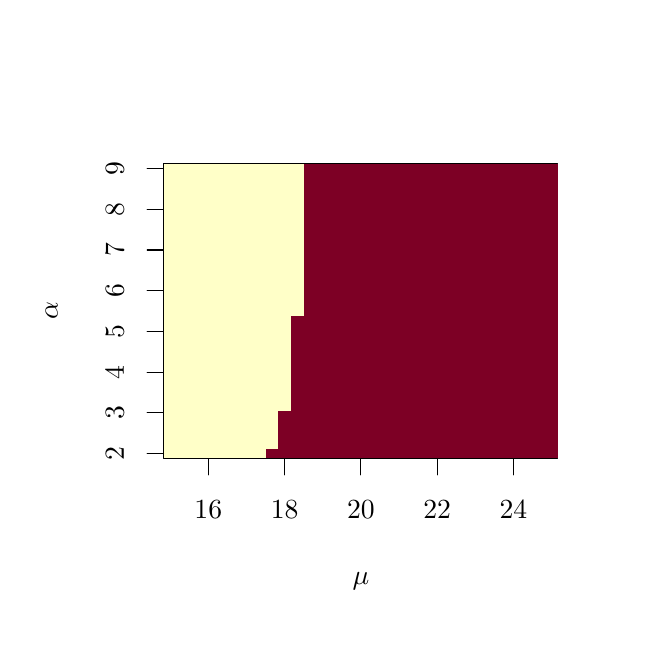
\begin{tikzpicture}[x=1pt,y=1pt]
\definecolor{fillColor}{RGB}{255,255,255}
\path[use as bounding box,fill=fillColor,fill opacity=0.00] (0,0) rectangle (216.81,216.81);
\begin{scope}
\path[clip] (  0.00,  0.00) rectangle (216.81,216.81);
\definecolor{drawColor}{RGB}{0,0,0}

\path[draw=drawColor,line width= 0.4pt,line join=round,line cap=round] ( 65.28, 61.20) -- (175.53, 61.20);

\path[draw=drawColor,line width= 0.4pt,line join=round,line cap=round] ( 65.28, 61.20) -- ( 65.28, 55.20);

\path[draw=drawColor,line width= 0.4pt,line join=round,line cap=round] ( 92.84, 61.20) -- ( 92.84, 55.20);

\path[draw=drawColor,line width= 0.4pt,line join=round,line cap=round] (120.40, 61.20) -- (120.40, 55.20);

\path[draw=drawColor,line width= 0.4pt,line join=round,line cap=round] (147.97, 61.20) -- (147.97, 55.20);

\path[draw=drawColor,line width= 0.4pt,line join=round,line cap=round] (175.53, 61.20) -- (175.53, 55.20);

\node[text=drawColor,anchor=base,inner sep=0pt, outer sep=0pt, scale=  1.00] at ( 65.28, 39.60) {16};

\node[text=drawColor,anchor=base,inner sep=0pt, outer sep=0pt, scale=  1.00] at ( 92.84, 39.60) {18};

\node[text=drawColor,anchor=base,inner sep=0pt, outer sep=0pt, scale=  1.00] at (120.40, 39.60) {20};

\node[text=drawColor,anchor=base,inner sep=0pt, outer sep=0pt, scale=  1.00] at (147.97, 39.60) {22};

\node[text=drawColor,anchor=base,inner sep=0pt, outer sep=0pt, scale=  1.00] at (175.53, 39.60) {24};

\path[draw=drawColor,line width= 0.4pt,line join=round,line cap=round] ( 49.20, 62.92) -- ( 49.20,165.89);

\path[draw=drawColor,line width= 0.4pt,line join=round,line cap=round] ( 49.20, 62.92) -- ( 43.20, 62.92);

\path[draw=drawColor,line width= 0.4pt,line join=round,line cap=round] ( 49.20, 77.63) -- ( 43.20, 77.63);

\path[draw=drawColor,line width= 0.4pt,line join=round,line cap=round] ( 49.20, 92.34) -- ( 43.20, 92.34);

\path[draw=drawColor,line width= 0.4pt,line join=round,line cap=round] ( 49.20,107.05) -- ( 43.20,107.05);

\path[draw=drawColor,line width= 0.4pt,line join=round,line cap=round] ( 49.20,121.76) -- ( 43.20,121.76);

\path[draw=drawColor,line width= 0.4pt,line join=round,line cap=round] ( 49.20,136.47) -- ( 43.20,136.47);

\path[draw=drawColor,line width= 0.4pt,line join=round,line cap=round] ( 49.20,151.18) -- ( 43.20,151.18);

\path[draw=drawColor,line width= 0.4pt,line join=round,line cap=round] ( 49.20,165.89) -- ( 43.20,165.89);

\node[text=drawColor,rotate= 90.00,anchor=base,inner sep=0pt, outer sep=0pt, scale=  1.00] at ( 34.80, 62.92) {2};

\node[text=drawColor,rotate= 90.00,anchor=base,inner sep=0pt, outer sep=0pt, scale=  1.00] at ( 34.80, 77.63) {3};

\node[text=drawColor,rotate= 90.00,anchor=base,inner sep=0pt, outer sep=0pt, scale=  1.00] at ( 34.80, 92.34) {4};

\node[text=drawColor,rotate= 90.00,anchor=base,inner sep=0pt, outer sep=0pt, scale=  1.00] at ( 34.80,107.05) {5};

\node[text=drawColor,rotate= 90.00,anchor=base,inner sep=0pt, outer sep=0pt, scale=  1.00] at ( 34.80,121.76) {6};

\node[text=drawColor,rotate= 90.00,anchor=base,inner sep=0pt, outer sep=0pt, scale=  1.00] at ( 34.80,136.47) {7};

\node[text=drawColor,rotate= 90.00,anchor=base,inner sep=0pt, outer sep=0pt, scale=  1.00] at ( 34.80,151.18) {8};

\node[text=drawColor,rotate= 90.00,anchor=base,inner sep=0pt, outer sep=0pt, scale=  1.00] at ( 34.80,165.89) {9};

\path[draw=drawColor,line width= 0.4pt,line join=round,line cap=round] ( 49.20, 61.20) --
	(191.61, 61.20) --
	(191.61,167.61) --
	( 49.20,167.61) --
	( 49.20, 61.20);
\end{scope}
\begin{scope}
\path[clip] (  0.00,  0.00) rectangle (216.81,216.81);
\definecolor{drawColor}{RGB}{0,0,0}

\node[text=drawColor,anchor=base,inner sep=0pt, outer sep=0pt, scale=  1.00] at (120.40, 15.60) {$\mu$};

\node[text=drawColor,rotate= 90.00,anchor=base,inner sep=0pt, outer sep=0pt, scale=  1.00] at ( 10.80,114.41) {$\alpha$};
\end{scope}
\begin{scope}
\path[clip] ( 49.20, 61.20) rectangle (191.61,167.61);
\definecolor{fillColor}{RGB}{255,255,200}

\path[fill=fillColor] ( 49.20, 61.20) rectangle ( 53.79, 64.63);

\path[fill=fillColor] ( 49.20, 64.63) rectangle ( 53.79, 68.07);

\path[fill=fillColor] ( 49.20, 68.07) rectangle ( 53.79, 71.50);

\path[fill=fillColor] ( 49.20, 71.50) rectangle ( 53.79, 74.93);

\path[fill=fillColor] ( 49.20, 74.93) rectangle ( 53.79, 78.36);

\path[fill=fillColor] ( 49.20, 78.36) rectangle ( 53.79, 81.80);

\path[fill=fillColor] ( 49.20, 81.80) rectangle ( 53.79, 85.23);

\path[fill=fillColor] ( 49.20, 85.23) rectangle ( 53.79, 88.66);

\path[fill=fillColor] ( 49.20, 88.66) rectangle ( 53.79, 92.09);

\path[fill=fillColor] ( 49.20, 92.09) rectangle ( 53.79, 95.53);

\path[fill=fillColor] ( 49.20, 95.53) rectangle ( 53.79, 98.96);

\path[fill=fillColor] ( 49.20, 98.96) rectangle ( 53.79,102.39);

\path[fill=fillColor] ( 49.20,102.39) rectangle ( 53.79,105.82);

\path[fill=fillColor] ( 49.20,105.82) rectangle ( 53.79,109.26);

\path[fill=fillColor] ( 49.20,109.26) rectangle ( 53.79,112.69);

\path[fill=fillColor] ( 49.20,112.69) rectangle ( 53.79,116.12);

\path[fill=fillColor] ( 49.20,116.12) rectangle ( 53.79,119.55);

\path[fill=fillColor] ( 49.20,119.55) rectangle ( 53.79,122.99);

\path[fill=fillColor] ( 49.20,122.99) rectangle ( 53.79,126.42);

\path[fill=fillColor] ( 49.20,126.42) rectangle ( 53.79,129.85);

\path[fill=fillColor] ( 49.20,129.85) rectangle ( 53.79,133.28);

\path[fill=fillColor] ( 49.20,133.28) rectangle ( 53.79,136.72);

\path[fill=fillColor] ( 49.20,136.72) rectangle ( 53.79,140.15);

\path[fill=fillColor] ( 49.20,140.15) rectangle ( 53.79,143.58);

\path[fill=fillColor] ( 49.20,143.58) rectangle ( 53.79,147.01);

\path[fill=fillColor] ( 49.20,147.01) rectangle ( 53.79,150.45);

\path[fill=fillColor] ( 49.20,150.45) rectangle ( 53.79,153.88);

\path[fill=fillColor] ( 49.20,153.88) rectangle ( 53.79,157.31);

\path[fill=fillColor] ( 49.20,157.31) rectangle ( 53.79,160.74);

\path[fill=fillColor] ( 49.20,160.74) rectangle ( 53.79,164.18);

\path[fill=fillColor] ( 49.20,164.18) rectangle ( 53.79,167.61);

\path[fill=fillColor] ( 53.79, 61.20) rectangle ( 58.39, 64.63);

\path[fill=fillColor] ( 53.79, 64.63) rectangle ( 58.39, 68.07);

\path[fill=fillColor] ( 53.79, 68.07) rectangle ( 58.39, 71.50);

\path[fill=fillColor] ( 53.79, 71.50) rectangle ( 58.39, 74.93);

\path[fill=fillColor] ( 53.79, 74.93) rectangle ( 58.39, 78.36);

\path[fill=fillColor] ( 53.79, 78.36) rectangle ( 58.39, 81.80);

\path[fill=fillColor] ( 53.79, 81.80) rectangle ( 58.39, 85.23);

\path[fill=fillColor] ( 53.79, 85.23) rectangle ( 58.39, 88.66);

\path[fill=fillColor] ( 53.79, 88.66) rectangle ( 58.39, 92.09);

\path[fill=fillColor] ( 53.79, 92.09) rectangle ( 58.39, 95.53);

\path[fill=fillColor] ( 53.79, 95.53) rectangle ( 58.39, 98.96);

\path[fill=fillColor] ( 53.79, 98.96) rectangle ( 58.39,102.39);

\path[fill=fillColor] ( 53.79,102.39) rectangle ( 58.39,105.82);

\path[fill=fillColor] ( 53.79,105.82) rectangle ( 58.39,109.26);

\path[fill=fillColor] ( 53.79,109.26) rectangle ( 58.39,112.69);

\path[fill=fillColor] ( 53.79,112.69) rectangle ( 58.39,116.12);

\path[fill=fillColor] ( 53.79,116.12) rectangle ( 58.39,119.55);

\path[fill=fillColor] ( 53.79,119.55) rectangle ( 58.39,122.99);

\path[fill=fillColor] ( 53.79,122.99) rectangle ( 58.39,126.42);

\path[fill=fillColor] ( 53.79,126.42) rectangle ( 58.39,129.85);

\path[fill=fillColor] ( 53.79,129.85) rectangle ( 58.39,133.28);

\path[fill=fillColor] ( 53.79,133.28) rectangle ( 58.39,136.72);

\path[fill=fillColor] ( 53.79,136.72) rectangle ( 58.39,140.15);

\path[fill=fillColor] ( 53.79,140.15) rectangle ( 58.39,143.58);

\path[fill=fillColor] ( 53.79,143.58) rectangle ( 58.39,147.01);

\path[fill=fillColor] ( 53.79,147.01) rectangle ( 58.39,150.45);

\path[fill=fillColor] ( 53.79,150.45) rectangle ( 58.39,153.88);

\path[fill=fillColor] ( 53.79,153.88) rectangle ( 58.39,157.31);

\path[fill=fillColor] ( 53.79,157.31) rectangle ( 58.39,160.74);

\path[fill=fillColor] ( 53.79,160.74) rectangle ( 58.39,164.18);

\path[fill=fillColor] ( 53.79,164.18) rectangle ( 58.39,167.61);

\path[fill=fillColor] ( 58.39, 61.20) rectangle ( 62.98, 64.63);

\path[fill=fillColor] ( 58.39, 64.63) rectangle ( 62.98, 68.07);

\path[fill=fillColor] ( 58.39, 68.07) rectangle ( 62.98, 71.50);

\path[fill=fillColor] ( 58.39, 71.50) rectangle ( 62.98, 74.93);

\path[fill=fillColor] ( 58.39, 74.93) rectangle ( 62.98, 78.36);

\path[fill=fillColor] ( 58.39, 78.36) rectangle ( 62.98, 81.80);

\path[fill=fillColor] ( 58.39, 81.80) rectangle ( 62.98, 85.23);

\path[fill=fillColor] ( 58.39, 85.23) rectangle ( 62.98, 88.66);

\path[fill=fillColor] ( 58.39, 88.66) rectangle ( 62.98, 92.09);

\path[fill=fillColor] ( 58.39, 92.09) rectangle ( 62.98, 95.53);

\path[fill=fillColor] ( 58.39, 95.53) rectangle ( 62.98, 98.96);

\path[fill=fillColor] ( 58.39, 98.96) rectangle ( 62.98,102.39);

\path[fill=fillColor] ( 58.39,102.39) rectangle ( 62.98,105.82);

\path[fill=fillColor] ( 58.39,105.82) rectangle ( 62.98,109.26);

\path[fill=fillColor] ( 58.39,109.26) rectangle ( 62.98,112.69);

\path[fill=fillColor] ( 58.39,112.69) rectangle ( 62.98,116.12);

\path[fill=fillColor] ( 58.39,116.12) rectangle ( 62.98,119.55);

\path[fill=fillColor] ( 58.39,119.55) rectangle ( 62.98,122.99);

\path[fill=fillColor] ( 58.39,122.99) rectangle ( 62.98,126.42);

\path[fill=fillColor] ( 58.39,126.42) rectangle ( 62.98,129.85);

\path[fill=fillColor] ( 58.39,129.85) rectangle ( 62.98,133.28);

\path[fill=fillColor] ( 58.39,133.28) rectangle ( 62.98,136.72);

\path[fill=fillColor] ( 58.39,136.72) rectangle ( 62.98,140.15);

\path[fill=fillColor] ( 58.39,140.15) rectangle ( 62.98,143.58);

\path[fill=fillColor] ( 58.39,143.58) rectangle ( 62.98,147.01);

\path[fill=fillColor] ( 58.39,147.01) rectangle ( 62.98,150.45);

\path[fill=fillColor] ( 58.39,150.45) rectangle ( 62.98,153.88);

\path[fill=fillColor] ( 58.39,153.88) rectangle ( 62.98,157.31);

\path[fill=fillColor] ( 58.39,157.31) rectangle ( 62.98,160.74);

\path[fill=fillColor] ( 58.39,160.74) rectangle ( 62.98,164.18);

\path[fill=fillColor] ( 58.39,164.18) rectangle ( 62.98,167.61);

\path[fill=fillColor] ( 62.98, 61.20) rectangle ( 67.58, 64.63);

\path[fill=fillColor] ( 62.98, 64.63) rectangle ( 67.58, 68.07);

\path[fill=fillColor] ( 62.98, 68.07) rectangle ( 67.58, 71.50);

\path[fill=fillColor] ( 62.98, 71.50) rectangle ( 67.58, 74.93);

\path[fill=fillColor] ( 62.98, 74.93) rectangle ( 67.58, 78.36);

\path[fill=fillColor] ( 62.98, 78.36) rectangle ( 67.58, 81.80);

\path[fill=fillColor] ( 62.98, 81.80) rectangle ( 67.58, 85.23);

\path[fill=fillColor] ( 62.98, 85.23) rectangle ( 67.58, 88.66);

\path[fill=fillColor] ( 62.98, 88.66) rectangle ( 67.58, 92.09);

\path[fill=fillColor] ( 62.98, 92.09) rectangle ( 67.58, 95.53);

\path[fill=fillColor] ( 62.98, 95.53) rectangle ( 67.58, 98.96);

\path[fill=fillColor] ( 62.98, 98.96) rectangle ( 67.58,102.39);

\path[fill=fillColor] ( 62.98,102.39) rectangle ( 67.58,105.82);

\path[fill=fillColor] ( 62.98,105.82) rectangle ( 67.58,109.26);

\path[fill=fillColor] ( 62.98,109.26) rectangle ( 67.58,112.69);

\path[fill=fillColor] ( 62.98,112.69) rectangle ( 67.58,116.12);

\path[fill=fillColor] ( 62.98,116.12) rectangle ( 67.58,119.55);

\path[fill=fillColor] ( 62.98,119.55) rectangle ( 67.58,122.99);

\path[fill=fillColor] ( 62.98,122.99) rectangle ( 67.58,126.42);

\path[fill=fillColor] ( 62.98,126.42) rectangle ( 67.58,129.85);

\path[fill=fillColor] ( 62.98,129.85) rectangle ( 67.58,133.28);

\path[fill=fillColor] ( 62.98,133.28) rectangle ( 67.58,136.72);

\path[fill=fillColor] ( 62.98,136.72) rectangle ( 67.58,140.15);

\path[fill=fillColor] ( 62.98,140.15) rectangle ( 67.58,143.58);

\path[fill=fillColor] ( 62.98,143.58) rectangle ( 67.58,147.01);

\path[fill=fillColor] ( 62.98,147.01) rectangle ( 67.58,150.45);

\path[fill=fillColor] ( 62.98,150.45) rectangle ( 67.58,153.88);

\path[fill=fillColor] ( 62.98,153.88) rectangle ( 67.58,157.31);

\path[fill=fillColor] ( 62.98,157.31) rectangle ( 67.58,160.74);

\path[fill=fillColor] ( 62.98,160.74) rectangle ( 67.58,164.18);

\path[fill=fillColor] ( 62.98,164.18) rectangle ( 67.58,167.61);

\path[fill=fillColor] ( 67.58, 61.20) rectangle ( 72.17, 64.63);

\path[fill=fillColor] ( 67.58, 64.63) rectangle ( 72.17, 68.07);

\path[fill=fillColor] ( 67.58, 68.07) rectangle ( 72.17, 71.50);

\path[fill=fillColor] ( 67.58, 71.50) rectangle ( 72.17, 74.93);

\path[fill=fillColor] ( 67.58, 74.93) rectangle ( 72.17, 78.36);

\path[fill=fillColor] ( 67.58, 78.36) rectangle ( 72.17, 81.80);

\path[fill=fillColor] ( 67.58, 81.80) rectangle ( 72.17, 85.23);

\path[fill=fillColor] ( 67.58, 85.23) rectangle ( 72.17, 88.66);

\path[fill=fillColor] ( 67.58, 88.66) rectangle ( 72.17, 92.09);

\path[fill=fillColor] ( 67.58, 92.09) rectangle ( 72.17, 95.53);

\path[fill=fillColor] ( 67.58, 95.53) rectangle ( 72.17, 98.96);

\path[fill=fillColor] ( 67.58, 98.96) rectangle ( 72.17,102.39);

\path[fill=fillColor] ( 67.58,102.39) rectangle ( 72.17,105.82);

\path[fill=fillColor] ( 67.58,105.82) rectangle ( 72.17,109.26);

\path[fill=fillColor] ( 67.58,109.26) rectangle ( 72.17,112.69);

\path[fill=fillColor] ( 67.58,112.69) rectangle ( 72.17,116.12);

\path[fill=fillColor] ( 67.58,116.12) rectangle ( 72.17,119.55);

\path[fill=fillColor] ( 67.58,119.55) rectangle ( 72.17,122.99);

\path[fill=fillColor] ( 67.58,122.99) rectangle ( 72.17,126.42);

\path[fill=fillColor] ( 67.58,126.42) rectangle ( 72.17,129.85);

\path[fill=fillColor] ( 67.58,129.85) rectangle ( 72.17,133.28);

\path[fill=fillColor] ( 67.58,133.28) rectangle ( 72.17,136.72);

\path[fill=fillColor] ( 67.58,136.72) rectangle ( 72.17,140.15);

\path[fill=fillColor] ( 67.58,140.15) rectangle ( 72.17,143.58);

\path[fill=fillColor] ( 67.58,143.58) rectangle ( 72.17,147.01);

\path[fill=fillColor] ( 67.58,147.01) rectangle ( 72.17,150.45);

\path[fill=fillColor] ( 67.58,150.45) rectangle ( 72.17,153.88);

\path[fill=fillColor] ( 67.58,153.88) rectangle ( 72.17,157.31);

\path[fill=fillColor] ( 67.58,157.31) rectangle ( 72.17,160.74);

\path[fill=fillColor] ( 67.58,160.74) rectangle ( 72.17,164.18);

\path[fill=fillColor] ( 67.58,164.18) rectangle ( 72.17,167.61);

\path[fill=fillColor] ( 72.17, 61.20) rectangle ( 76.76, 64.63);

\path[fill=fillColor] ( 72.17, 64.63) rectangle ( 76.76, 68.07);

\path[fill=fillColor] ( 72.17, 68.07) rectangle ( 76.76, 71.50);

\path[fill=fillColor] ( 72.17, 71.50) rectangle ( 76.76, 74.93);

\path[fill=fillColor] ( 72.17, 74.93) rectangle ( 76.76, 78.36);

\path[fill=fillColor] ( 72.17, 78.36) rectangle ( 76.76, 81.80);

\path[fill=fillColor] ( 72.17, 81.80) rectangle ( 76.76, 85.23);

\path[fill=fillColor] ( 72.17, 85.23) rectangle ( 76.76, 88.66);

\path[fill=fillColor] ( 72.17, 88.66) rectangle ( 76.76, 92.09);

\path[fill=fillColor] ( 72.17, 92.09) rectangle ( 76.76, 95.53);

\path[fill=fillColor] ( 72.17, 95.53) rectangle ( 76.76, 98.96);

\path[fill=fillColor] ( 72.17, 98.96) rectangle ( 76.76,102.39);

\path[fill=fillColor] ( 72.17,102.39) rectangle ( 76.76,105.82);

\path[fill=fillColor] ( 72.17,105.82) rectangle ( 76.76,109.26);

\path[fill=fillColor] ( 72.17,109.26) rectangle ( 76.76,112.69);

\path[fill=fillColor] ( 72.17,112.69) rectangle ( 76.76,116.12);

\path[fill=fillColor] ( 72.17,116.12) rectangle ( 76.76,119.55);

\path[fill=fillColor] ( 72.17,119.55) rectangle ( 76.76,122.99);

\path[fill=fillColor] ( 72.17,122.99) rectangle ( 76.76,126.42);

\path[fill=fillColor] ( 72.17,126.42) rectangle ( 76.76,129.85);

\path[fill=fillColor] ( 72.17,129.85) rectangle ( 76.76,133.28);

\path[fill=fillColor] ( 72.17,133.28) rectangle ( 76.76,136.72);

\path[fill=fillColor] ( 72.17,136.72) rectangle ( 76.76,140.15);

\path[fill=fillColor] ( 72.17,140.15) rectangle ( 76.76,143.58);

\path[fill=fillColor] ( 72.17,143.58) rectangle ( 76.76,147.01);

\path[fill=fillColor] ( 72.17,147.01) rectangle ( 76.76,150.45);

\path[fill=fillColor] ( 72.17,150.45) rectangle ( 76.76,153.88);

\path[fill=fillColor] ( 72.17,153.88) rectangle ( 76.76,157.31);

\path[fill=fillColor] ( 72.17,157.31) rectangle ( 76.76,160.74);

\path[fill=fillColor] ( 72.17,160.74) rectangle ( 76.76,164.18);

\path[fill=fillColor] ( 72.17,164.18) rectangle ( 76.76,167.61);

\path[fill=fillColor] ( 76.76, 61.20) rectangle ( 81.36, 64.63);

\path[fill=fillColor] ( 76.76, 64.63) rectangle ( 81.36, 68.07);

\path[fill=fillColor] ( 76.76, 68.07) rectangle ( 81.36, 71.50);

\path[fill=fillColor] ( 76.76, 71.50) rectangle ( 81.36, 74.93);

\path[fill=fillColor] ( 76.76, 74.93) rectangle ( 81.36, 78.36);

\path[fill=fillColor] ( 76.76, 78.36) rectangle ( 81.36, 81.80);

\path[fill=fillColor] ( 76.76, 81.80) rectangle ( 81.36, 85.23);

\path[fill=fillColor] ( 76.76, 85.23) rectangle ( 81.36, 88.66);

\path[fill=fillColor] ( 76.76, 88.66) rectangle ( 81.36, 92.09);

\path[fill=fillColor] ( 76.76, 92.09) rectangle ( 81.36, 95.53);

\path[fill=fillColor] ( 76.76, 95.53) rectangle ( 81.36, 98.96);

\path[fill=fillColor] ( 76.76, 98.96) rectangle ( 81.36,102.39);

\path[fill=fillColor] ( 76.76,102.39) rectangle ( 81.36,105.82);

\path[fill=fillColor] ( 76.76,105.82) rectangle ( 81.36,109.26);

\path[fill=fillColor] ( 76.76,109.26) rectangle ( 81.36,112.69);

\path[fill=fillColor] ( 76.76,112.69) rectangle ( 81.36,116.12);

\path[fill=fillColor] ( 76.76,116.12) rectangle ( 81.36,119.55);

\path[fill=fillColor] ( 76.76,119.55) rectangle ( 81.36,122.99);

\path[fill=fillColor] ( 76.76,122.99) rectangle ( 81.36,126.42);

\path[fill=fillColor] ( 76.76,126.42) rectangle ( 81.36,129.85);

\path[fill=fillColor] ( 76.76,129.85) rectangle ( 81.36,133.28);

\path[fill=fillColor] ( 76.76,133.28) rectangle ( 81.36,136.72);

\path[fill=fillColor] ( 76.76,136.72) rectangle ( 81.36,140.15);

\path[fill=fillColor] ( 76.76,140.15) rectangle ( 81.36,143.58);

\path[fill=fillColor] ( 76.76,143.58) rectangle ( 81.36,147.01);

\path[fill=fillColor] ( 76.76,147.01) rectangle ( 81.36,150.45);

\path[fill=fillColor] ( 76.76,150.45) rectangle ( 81.36,153.88);

\path[fill=fillColor] ( 76.76,153.88) rectangle ( 81.36,157.31);

\path[fill=fillColor] ( 76.76,157.31) rectangle ( 81.36,160.74);

\path[fill=fillColor] ( 76.76,160.74) rectangle ( 81.36,164.18);

\path[fill=fillColor] ( 76.76,164.18) rectangle ( 81.36,167.61);

\path[fill=fillColor] ( 81.36, 61.20) rectangle ( 85.95, 64.63);

\path[fill=fillColor] ( 81.36, 64.63) rectangle ( 85.95, 68.07);

\path[fill=fillColor] ( 81.36, 68.07) rectangle ( 85.95, 71.50);

\path[fill=fillColor] ( 81.36, 71.50) rectangle ( 85.95, 74.93);

\path[fill=fillColor] ( 81.36, 74.93) rectangle ( 85.95, 78.36);

\path[fill=fillColor] ( 81.36, 78.36) rectangle ( 85.95, 81.80);

\path[fill=fillColor] ( 81.36, 81.80) rectangle ( 85.95, 85.23);

\path[fill=fillColor] ( 81.36, 85.23) rectangle ( 85.95, 88.66);

\path[fill=fillColor] ( 81.36, 88.66) rectangle ( 85.95, 92.09);

\path[fill=fillColor] ( 81.36, 92.09) rectangle ( 85.95, 95.53);

\path[fill=fillColor] ( 81.36, 95.53) rectangle ( 85.95, 98.96);

\path[fill=fillColor] ( 81.36, 98.96) rectangle ( 85.95,102.39);

\path[fill=fillColor] ( 81.36,102.39) rectangle ( 85.95,105.82);

\path[fill=fillColor] ( 81.36,105.82) rectangle ( 85.95,109.26);

\path[fill=fillColor] ( 81.36,109.26) rectangle ( 85.95,112.69);

\path[fill=fillColor] ( 81.36,112.69) rectangle ( 85.95,116.12);

\path[fill=fillColor] ( 81.36,116.12) rectangle ( 85.95,119.55);

\path[fill=fillColor] ( 81.36,119.55) rectangle ( 85.95,122.99);

\path[fill=fillColor] ( 81.36,122.99) rectangle ( 85.95,126.42);

\path[fill=fillColor] ( 81.36,126.42) rectangle ( 85.95,129.85);

\path[fill=fillColor] ( 81.36,129.85) rectangle ( 85.95,133.28);

\path[fill=fillColor] ( 81.36,133.28) rectangle ( 85.95,136.72);

\path[fill=fillColor] ( 81.36,136.72) rectangle ( 85.95,140.15);

\path[fill=fillColor] ( 81.36,140.15) rectangle ( 85.95,143.58);

\path[fill=fillColor] ( 81.36,143.58) rectangle ( 85.95,147.01);

\path[fill=fillColor] ( 81.36,147.01) rectangle ( 85.95,150.45);

\path[fill=fillColor] ( 81.36,150.45) rectangle ( 85.95,153.88);

\path[fill=fillColor] ( 81.36,153.88) rectangle ( 85.95,157.31);

\path[fill=fillColor] ( 81.36,157.31) rectangle ( 85.95,160.74);

\path[fill=fillColor] ( 81.36,160.74) rectangle ( 85.95,164.18);

\path[fill=fillColor] ( 81.36,164.18) rectangle ( 85.95,167.61);
\definecolor{fillColor}{RGB}{125,0,37}

\path[fill=fillColor] ( 85.95, 61.20) rectangle ( 90.54, 64.63);
\definecolor{fillColor}{RGB}{255,255,200}

\path[fill=fillColor] ( 85.95, 64.63) rectangle ( 90.54, 68.07);

\path[fill=fillColor] ( 85.95, 68.07) rectangle ( 90.54, 71.50);

\path[fill=fillColor] ( 85.95, 71.50) rectangle ( 90.54, 74.93);

\path[fill=fillColor] ( 85.95, 74.93) rectangle ( 90.54, 78.36);

\path[fill=fillColor] ( 85.95, 78.36) rectangle ( 90.54, 81.80);

\path[fill=fillColor] ( 85.95, 81.80) rectangle ( 90.54, 85.23);

\path[fill=fillColor] ( 85.95, 85.23) rectangle ( 90.54, 88.66);

\path[fill=fillColor] ( 85.95, 88.66) rectangle ( 90.54, 92.09);

\path[fill=fillColor] ( 85.95, 92.09) rectangle ( 90.54, 95.53);

\path[fill=fillColor] ( 85.95, 95.53) rectangle ( 90.54, 98.96);

\path[fill=fillColor] ( 85.95, 98.96) rectangle ( 90.54,102.39);

\path[fill=fillColor] ( 85.95,102.39) rectangle ( 90.54,105.82);

\path[fill=fillColor] ( 85.95,105.82) rectangle ( 90.54,109.26);

\path[fill=fillColor] ( 85.95,109.26) rectangle ( 90.54,112.69);

\path[fill=fillColor] ( 85.95,112.69) rectangle ( 90.54,116.12);

\path[fill=fillColor] ( 85.95,116.12) rectangle ( 90.54,119.55);

\path[fill=fillColor] ( 85.95,119.55) rectangle ( 90.54,122.99);

\path[fill=fillColor] ( 85.95,122.99) rectangle ( 90.54,126.42);

\path[fill=fillColor] ( 85.95,126.42) rectangle ( 90.54,129.85);

\path[fill=fillColor] ( 85.95,129.85) rectangle ( 90.54,133.28);

\path[fill=fillColor] ( 85.95,133.28) rectangle ( 90.54,136.72);

\path[fill=fillColor] ( 85.95,136.72) rectangle ( 90.54,140.15);

\path[fill=fillColor] ( 85.95,140.15) rectangle ( 90.54,143.58);

\path[fill=fillColor] ( 85.95,143.58) rectangle ( 90.54,147.01);

\path[fill=fillColor] ( 85.95,147.01) rectangle ( 90.54,150.45);

\path[fill=fillColor] ( 85.95,150.45) rectangle ( 90.54,153.88);

\path[fill=fillColor] ( 85.95,153.88) rectangle ( 90.54,157.31);

\path[fill=fillColor] ( 85.95,157.31) rectangle ( 90.54,160.74);

\path[fill=fillColor] ( 85.95,160.74) rectangle ( 90.54,164.18);

\path[fill=fillColor] ( 85.95,164.18) rectangle ( 90.54,167.61);
\definecolor{fillColor}{RGB}{125,0,37}

\path[fill=fillColor] ( 90.54, 61.20) rectangle ( 95.14, 64.63);

\path[fill=fillColor] ( 90.54, 64.63) rectangle ( 95.14, 68.07);

\path[fill=fillColor] ( 90.54, 68.07) rectangle ( 95.14, 71.50);

\path[fill=fillColor] ( 90.54, 71.50) rectangle ( 95.14, 74.93);

\path[fill=fillColor] ( 90.54, 74.93) rectangle ( 95.14, 78.36);
\definecolor{fillColor}{RGB}{255,255,200}

\path[fill=fillColor] ( 90.54, 78.36) rectangle ( 95.14, 81.80);

\path[fill=fillColor] ( 90.54, 81.80) rectangle ( 95.14, 85.23);

\path[fill=fillColor] ( 90.54, 85.23) rectangle ( 95.14, 88.66);

\path[fill=fillColor] ( 90.54, 88.66) rectangle ( 95.14, 92.09);

\path[fill=fillColor] ( 90.54, 92.09) rectangle ( 95.14, 95.53);

\path[fill=fillColor] ( 90.54, 95.53) rectangle ( 95.14, 98.96);

\path[fill=fillColor] ( 90.54, 98.96) rectangle ( 95.14,102.39);

\path[fill=fillColor] ( 90.54,102.39) rectangle ( 95.14,105.82);

\path[fill=fillColor] ( 90.54,105.82) rectangle ( 95.14,109.26);

\path[fill=fillColor] ( 90.54,109.26) rectangle ( 95.14,112.69);

\path[fill=fillColor] ( 90.54,112.69) rectangle ( 95.14,116.12);

\path[fill=fillColor] ( 90.54,116.12) rectangle ( 95.14,119.55);

\path[fill=fillColor] ( 90.54,119.55) rectangle ( 95.14,122.99);

\path[fill=fillColor] ( 90.54,122.99) rectangle ( 95.14,126.42);

\path[fill=fillColor] ( 90.54,126.42) rectangle ( 95.14,129.85);

\path[fill=fillColor] ( 90.54,129.85) rectangle ( 95.14,133.28);

\path[fill=fillColor] ( 90.54,133.28) rectangle ( 95.14,136.72);

\path[fill=fillColor] ( 90.54,136.72) rectangle ( 95.14,140.15);

\path[fill=fillColor] ( 90.54,140.15) rectangle ( 95.14,143.58);

\path[fill=fillColor] ( 90.54,143.58) rectangle ( 95.14,147.01);

\path[fill=fillColor] ( 90.54,147.01) rectangle ( 95.14,150.45);

\path[fill=fillColor] ( 90.54,150.45) rectangle ( 95.14,153.88);

\path[fill=fillColor] ( 90.54,153.88) rectangle ( 95.14,157.31);

\path[fill=fillColor] ( 90.54,157.31) rectangle ( 95.14,160.74);

\path[fill=fillColor] ( 90.54,160.74) rectangle ( 95.14,164.18);

\path[fill=fillColor] ( 90.54,164.18) rectangle ( 95.14,167.61);
\definecolor{fillColor}{RGB}{125,0,37}

\path[fill=fillColor] ( 95.14, 61.20) rectangle ( 99.73, 64.63);

\path[fill=fillColor] ( 95.14, 64.63) rectangle ( 99.73, 68.07);

\path[fill=fillColor] ( 95.14, 68.07) rectangle ( 99.73, 71.50);

\path[fill=fillColor] ( 95.14, 71.50) rectangle ( 99.73, 74.93);

\path[fill=fillColor] ( 95.14, 74.93) rectangle ( 99.73, 78.36);

\path[fill=fillColor] ( 95.14, 78.36) rectangle ( 99.73, 81.80);

\path[fill=fillColor] ( 95.14, 81.80) rectangle ( 99.73, 85.23);

\path[fill=fillColor] ( 95.14, 85.23) rectangle ( 99.73, 88.66);

\path[fill=fillColor] ( 95.14, 88.66) rectangle ( 99.73, 92.09);

\path[fill=fillColor] ( 95.14, 92.09) rectangle ( 99.73, 95.53);

\path[fill=fillColor] ( 95.14, 95.53) rectangle ( 99.73, 98.96);

\path[fill=fillColor] ( 95.14, 98.96) rectangle ( 99.73,102.39);

\path[fill=fillColor] ( 95.14,102.39) rectangle ( 99.73,105.82);

\path[fill=fillColor] ( 95.14,105.82) rectangle ( 99.73,109.26);

\path[fill=fillColor] ( 95.14,109.26) rectangle ( 99.73,112.69);
\definecolor{fillColor}{RGB}{255,255,200}

\path[fill=fillColor] ( 95.14,112.69) rectangle ( 99.73,116.12);

\path[fill=fillColor] ( 95.14,116.12) rectangle ( 99.73,119.55);

\path[fill=fillColor] ( 95.14,119.55) rectangle ( 99.73,122.99);

\path[fill=fillColor] ( 95.14,122.99) rectangle ( 99.73,126.42);

\path[fill=fillColor] ( 95.14,126.42) rectangle ( 99.73,129.85);

\path[fill=fillColor] ( 95.14,129.85) rectangle ( 99.73,133.28);

\path[fill=fillColor] ( 95.14,133.28) rectangle ( 99.73,136.72);

\path[fill=fillColor] ( 95.14,136.72) rectangle ( 99.73,140.15);

\path[fill=fillColor] ( 95.14,140.15) rectangle ( 99.73,143.58);

\path[fill=fillColor] ( 95.14,143.58) rectangle ( 99.73,147.01);

\path[fill=fillColor] ( 95.14,147.01) rectangle ( 99.73,150.45);

\path[fill=fillColor] ( 95.14,150.45) rectangle ( 99.73,153.88);

\path[fill=fillColor] ( 95.14,153.88) rectangle ( 99.73,157.31);

\path[fill=fillColor] ( 95.14,157.31) rectangle ( 99.73,160.74);

\path[fill=fillColor] ( 95.14,160.74) rectangle ( 99.73,164.18);

\path[fill=fillColor] ( 95.14,164.18) rectangle ( 99.73,167.61);
\definecolor{fillColor}{RGB}{125,0,37}

\path[fill=fillColor] ( 99.73, 61.20) rectangle (104.33, 64.63);

\path[fill=fillColor] ( 99.73, 64.63) rectangle (104.33, 68.07);

\path[fill=fillColor] ( 99.73, 68.07) rectangle (104.33, 71.50);

\path[fill=fillColor] ( 99.73, 71.50) rectangle (104.33, 74.93);

\path[fill=fillColor] ( 99.73, 74.93) rectangle (104.33, 78.36);

\path[fill=fillColor] ( 99.73, 78.36) rectangle (104.33, 81.80);

\path[fill=fillColor] ( 99.73, 81.80) rectangle (104.33, 85.23);

\path[fill=fillColor] ( 99.73, 85.23) rectangle (104.33, 88.66);

\path[fill=fillColor] ( 99.73, 88.66) rectangle (104.33, 92.09);

\path[fill=fillColor] ( 99.73, 92.09) rectangle (104.33, 95.53);

\path[fill=fillColor] ( 99.73, 95.53) rectangle (104.33, 98.96);

\path[fill=fillColor] ( 99.73, 98.96) rectangle (104.33,102.39);

\path[fill=fillColor] ( 99.73,102.39) rectangle (104.33,105.82);

\path[fill=fillColor] ( 99.73,105.82) rectangle (104.33,109.26);

\path[fill=fillColor] ( 99.73,109.26) rectangle (104.33,112.69);

\path[fill=fillColor] ( 99.73,112.69) rectangle (104.33,116.12);

\path[fill=fillColor] ( 99.73,116.12) rectangle (104.33,119.55);

\path[fill=fillColor] ( 99.73,119.55) rectangle (104.33,122.99);

\path[fill=fillColor] ( 99.73,122.99) rectangle (104.33,126.42);

\path[fill=fillColor] ( 99.73,126.42) rectangle (104.33,129.85);

\path[fill=fillColor] ( 99.73,129.85) rectangle (104.33,133.28);

\path[fill=fillColor] ( 99.73,133.28) rectangle (104.33,136.72);

\path[fill=fillColor] ( 99.73,136.72) rectangle (104.33,140.15);

\path[fill=fillColor] ( 99.73,140.15) rectangle (104.33,143.58);

\path[fill=fillColor] ( 99.73,143.58) rectangle (104.33,147.01);

\path[fill=fillColor] ( 99.73,147.01) rectangle (104.33,150.45);

\path[fill=fillColor] ( 99.73,150.45) rectangle (104.33,153.88);

\path[fill=fillColor] ( 99.73,153.88) rectangle (104.33,157.31);

\path[fill=fillColor] ( 99.73,157.31) rectangle (104.33,160.74);

\path[fill=fillColor] ( 99.73,160.74) rectangle (104.33,164.18);

\path[fill=fillColor] ( 99.73,164.18) rectangle (104.33,167.61);

\path[fill=fillColor] (104.33, 61.20) rectangle (108.92, 64.63);

\path[fill=fillColor] (104.33, 64.63) rectangle (108.92, 68.07);

\path[fill=fillColor] (104.33, 68.07) rectangle (108.92, 71.50);

\path[fill=fillColor] (104.33, 71.50) rectangle (108.92, 74.93);

\path[fill=fillColor] (104.33, 74.93) rectangle (108.92, 78.36);

\path[fill=fillColor] (104.33, 78.36) rectangle (108.92, 81.80);

\path[fill=fillColor] (104.33, 81.80) rectangle (108.92, 85.23);

\path[fill=fillColor] (104.33, 85.23) rectangle (108.92, 88.66);

\path[fill=fillColor] (104.33, 88.66) rectangle (108.92, 92.09);

\path[fill=fillColor] (104.33, 92.09) rectangle (108.92, 95.53);

\path[fill=fillColor] (104.33, 95.53) rectangle (108.92, 98.96);

\path[fill=fillColor] (104.33, 98.96) rectangle (108.92,102.39);

\path[fill=fillColor] (104.33,102.39) rectangle (108.92,105.82);

\path[fill=fillColor] (104.33,105.82) rectangle (108.92,109.26);

\path[fill=fillColor] (104.33,109.26) rectangle (108.92,112.69);

\path[fill=fillColor] (104.33,112.69) rectangle (108.92,116.12);

\path[fill=fillColor] (104.33,116.12) rectangle (108.92,119.55);

\path[fill=fillColor] (104.33,119.55) rectangle (108.92,122.99);

\path[fill=fillColor] (104.33,122.99) rectangle (108.92,126.42);

\path[fill=fillColor] (104.33,126.42) rectangle (108.92,129.85);

\path[fill=fillColor] (104.33,129.85) rectangle (108.92,133.28);

\path[fill=fillColor] (104.33,133.28) rectangle (108.92,136.72);

\path[fill=fillColor] (104.33,136.72) rectangle (108.92,140.15);

\path[fill=fillColor] (104.33,140.15) rectangle (108.92,143.58);

\path[fill=fillColor] (104.33,143.58) rectangle (108.92,147.01);

\path[fill=fillColor] (104.33,147.01) rectangle (108.92,150.45);

\path[fill=fillColor] (104.33,150.45) rectangle (108.92,153.88);

\path[fill=fillColor] (104.33,153.88) rectangle (108.92,157.31);

\path[fill=fillColor] (104.33,157.31) rectangle (108.92,160.74);

\path[fill=fillColor] (104.33,160.74) rectangle (108.92,164.18);

\path[fill=fillColor] (104.33,164.18) rectangle (108.92,167.61);

\path[fill=fillColor] (108.92, 61.20) rectangle (113.51, 64.63);

\path[fill=fillColor] (108.92, 64.63) rectangle (113.51, 68.07);

\path[fill=fillColor] (108.92, 68.07) rectangle (113.51, 71.50);

\path[fill=fillColor] (108.92, 71.50) rectangle (113.51, 74.93);

\path[fill=fillColor] (108.92, 74.93) rectangle (113.51, 78.36);

\path[fill=fillColor] (108.92, 78.36) rectangle (113.51, 81.80);

\path[fill=fillColor] (108.92, 81.80) rectangle (113.51, 85.23);

\path[fill=fillColor] (108.92, 85.23) rectangle (113.51, 88.66);

\path[fill=fillColor] (108.92, 88.66) rectangle (113.51, 92.09);

\path[fill=fillColor] (108.92, 92.09) rectangle (113.51, 95.53);

\path[fill=fillColor] (108.92, 95.53) rectangle (113.51, 98.96);

\path[fill=fillColor] (108.92, 98.96) rectangle (113.51,102.39);

\path[fill=fillColor] (108.92,102.39) rectangle (113.51,105.82);

\path[fill=fillColor] (108.92,105.82) rectangle (113.51,109.26);

\path[fill=fillColor] (108.92,109.26) rectangle (113.51,112.69);

\path[fill=fillColor] (108.92,112.69) rectangle (113.51,116.12);

\path[fill=fillColor] (108.92,116.12) rectangle (113.51,119.55);

\path[fill=fillColor] (108.92,119.55) rectangle (113.51,122.99);

\path[fill=fillColor] (108.92,122.99) rectangle (113.51,126.42);

\path[fill=fillColor] (108.92,126.42) rectangle (113.51,129.85);

\path[fill=fillColor] (108.92,129.85) rectangle (113.51,133.28);

\path[fill=fillColor] (108.92,133.28) rectangle (113.51,136.72);

\path[fill=fillColor] (108.92,136.72) rectangle (113.51,140.15);

\path[fill=fillColor] (108.92,140.15) rectangle (113.51,143.58);

\path[fill=fillColor] (108.92,143.58) rectangle (113.51,147.01);

\path[fill=fillColor] (108.92,147.01) rectangle (113.51,150.45);

\path[fill=fillColor] (108.92,150.45) rectangle (113.51,153.88);

\path[fill=fillColor] (108.92,153.88) rectangle (113.51,157.31);

\path[fill=fillColor] (108.92,157.31) rectangle (113.51,160.74);

\path[fill=fillColor] (108.92,160.74) rectangle (113.51,164.18);

\path[fill=fillColor] (108.92,164.18) rectangle (113.51,167.61);

\path[fill=fillColor] (113.51, 61.20) rectangle (118.11, 64.63);

\path[fill=fillColor] (113.51, 64.63) rectangle (118.11, 68.07);

\path[fill=fillColor] (113.51, 68.07) rectangle (118.11, 71.50);

\path[fill=fillColor] (113.51, 71.50) rectangle (118.11, 74.93);

\path[fill=fillColor] (113.51, 74.93) rectangle (118.11, 78.36);

\path[fill=fillColor] (113.51, 78.36) rectangle (118.11, 81.80);

\path[fill=fillColor] (113.51, 81.80) rectangle (118.11, 85.23);

\path[fill=fillColor] (113.51, 85.23) rectangle (118.11, 88.66);

\path[fill=fillColor] (113.51, 88.66) rectangle (118.11, 92.09);

\path[fill=fillColor] (113.51, 92.09) rectangle (118.11, 95.53);

\path[fill=fillColor] (113.51, 95.53) rectangle (118.11, 98.96);

\path[fill=fillColor] (113.51, 98.96) rectangle (118.11,102.39);

\path[fill=fillColor] (113.51,102.39) rectangle (118.11,105.82);

\path[fill=fillColor] (113.51,105.82) rectangle (118.11,109.26);

\path[fill=fillColor] (113.51,109.26) rectangle (118.11,112.69);

\path[fill=fillColor] (113.51,112.69) rectangle (118.11,116.12);

\path[fill=fillColor] (113.51,116.12) rectangle (118.11,119.55);

\path[fill=fillColor] (113.51,119.55) rectangle (118.11,122.99);

\path[fill=fillColor] (113.51,122.99) rectangle (118.11,126.42);

\path[fill=fillColor] (113.51,126.42) rectangle (118.11,129.85);

\path[fill=fillColor] (113.51,129.85) rectangle (118.11,133.28);

\path[fill=fillColor] (113.51,133.28) rectangle (118.11,136.72);

\path[fill=fillColor] (113.51,136.72) rectangle (118.11,140.15);

\path[fill=fillColor] (113.51,140.15) rectangle (118.11,143.58);

\path[fill=fillColor] (113.51,143.58) rectangle (118.11,147.01);

\path[fill=fillColor] (113.51,147.01) rectangle (118.11,150.45);

\path[fill=fillColor] (113.51,150.45) rectangle (118.11,153.88);

\path[fill=fillColor] (113.51,153.88) rectangle (118.11,157.31);

\path[fill=fillColor] (113.51,157.31) rectangle (118.11,160.74);

\path[fill=fillColor] (113.51,160.74) rectangle (118.11,164.18);

\path[fill=fillColor] (113.51,164.18) rectangle (118.11,167.61);

\path[fill=fillColor] (118.11, 61.20) rectangle (122.70, 64.63);

\path[fill=fillColor] (118.11, 64.63) rectangle (122.70, 68.07);

\path[fill=fillColor] (118.11, 68.07) rectangle (122.70, 71.50);

\path[fill=fillColor] (118.11, 71.50) rectangle (122.70, 74.93);

\path[fill=fillColor] (118.11, 74.93) rectangle (122.70, 78.36);

\path[fill=fillColor] (118.11, 78.36) rectangle (122.70, 81.80);

\path[fill=fillColor] (118.11, 81.80) rectangle (122.70, 85.23);

\path[fill=fillColor] (118.11, 85.23) rectangle (122.70, 88.66);

\path[fill=fillColor] (118.11, 88.66) rectangle (122.70, 92.09);

\path[fill=fillColor] (118.11, 92.09) rectangle (122.70, 95.53);

\path[fill=fillColor] (118.11, 95.53) rectangle (122.70, 98.96);

\path[fill=fillColor] (118.11, 98.96) rectangle (122.70,102.39);

\path[fill=fillColor] (118.11,102.39) rectangle (122.70,105.82);

\path[fill=fillColor] (118.11,105.82) rectangle (122.70,109.26);

\path[fill=fillColor] (118.11,109.26) rectangle (122.70,112.69);

\path[fill=fillColor] (118.11,112.69) rectangle (122.70,116.12);

\path[fill=fillColor] (118.11,116.12) rectangle (122.70,119.55);

\path[fill=fillColor] (118.11,119.55) rectangle (122.70,122.99);

\path[fill=fillColor] (118.11,122.99) rectangle (122.70,126.42);

\path[fill=fillColor] (118.11,126.42) rectangle (122.70,129.85);

\path[fill=fillColor] (118.11,129.85) rectangle (122.70,133.28);

\path[fill=fillColor] (118.11,133.28) rectangle (122.70,136.72);

\path[fill=fillColor] (118.11,136.72) rectangle (122.70,140.15);

\path[fill=fillColor] (118.11,140.15) rectangle (122.70,143.58);

\path[fill=fillColor] (118.11,143.58) rectangle (122.70,147.01);

\path[fill=fillColor] (118.11,147.01) rectangle (122.70,150.45);

\path[fill=fillColor] (118.11,150.45) rectangle (122.70,153.88);

\path[fill=fillColor] (118.11,153.88) rectangle (122.70,157.31);

\path[fill=fillColor] (118.11,157.31) rectangle (122.70,160.74);

\path[fill=fillColor] (118.11,160.74) rectangle (122.70,164.18);

\path[fill=fillColor] (118.11,164.18) rectangle (122.70,167.61);

\path[fill=fillColor] (122.70, 61.20) rectangle (127.30, 64.63);

\path[fill=fillColor] (122.70, 64.63) rectangle (127.30, 68.07);

\path[fill=fillColor] (122.70, 68.07) rectangle (127.30, 71.50);

\path[fill=fillColor] (122.70, 71.50) rectangle (127.30, 74.93);

\path[fill=fillColor] (122.70, 74.93) rectangle (127.30, 78.36);

\path[fill=fillColor] (122.70, 78.36) rectangle (127.30, 81.80);

\path[fill=fillColor] (122.70, 81.80) rectangle (127.30, 85.23);

\path[fill=fillColor] (122.70, 85.23) rectangle (127.30, 88.66);

\path[fill=fillColor] (122.70, 88.66) rectangle (127.30, 92.09);

\path[fill=fillColor] (122.70, 92.09) rectangle (127.30, 95.53);

\path[fill=fillColor] (122.70, 95.53) rectangle (127.30, 98.96);

\path[fill=fillColor] (122.70, 98.96) rectangle (127.30,102.39);

\path[fill=fillColor] (122.70,102.39) rectangle (127.30,105.82);

\path[fill=fillColor] (122.70,105.82) rectangle (127.30,109.26);

\path[fill=fillColor] (122.70,109.26) rectangle (127.30,112.69);

\path[fill=fillColor] (122.70,112.69) rectangle (127.30,116.12);

\path[fill=fillColor] (122.70,116.12) rectangle (127.30,119.55);

\path[fill=fillColor] (122.70,119.55) rectangle (127.30,122.99);

\path[fill=fillColor] (122.70,122.99) rectangle (127.30,126.42);

\path[fill=fillColor] (122.70,126.42) rectangle (127.30,129.85);

\path[fill=fillColor] (122.70,129.85) rectangle (127.30,133.28);

\path[fill=fillColor] (122.70,133.28) rectangle (127.30,136.72);

\path[fill=fillColor] (122.70,136.72) rectangle (127.30,140.15);

\path[fill=fillColor] (122.70,140.15) rectangle (127.30,143.58);

\path[fill=fillColor] (122.70,143.58) rectangle (127.30,147.01);

\path[fill=fillColor] (122.70,147.01) rectangle (127.30,150.45);

\path[fill=fillColor] (122.70,150.45) rectangle (127.30,153.88);

\path[fill=fillColor] (122.70,153.88) rectangle (127.30,157.31);

\path[fill=fillColor] (122.70,157.31) rectangle (127.30,160.74);

\path[fill=fillColor] (122.70,160.74) rectangle (127.30,164.18);

\path[fill=fillColor] (122.70,164.18) rectangle (127.30,167.61);

\path[fill=fillColor] (127.30, 61.20) rectangle (131.89, 64.63);

\path[fill=fillColor] (127.30, 64.63) rectangle (131.89, 68.07);

\path[fill=fillColor] (127.30, 68.07) rectangle (131.89, 71.50);

\path[fill=fillColor] (127.30, 71.50) rectangle (131.89, 74.93);

\path[fill=fillColor] (127.30, 74.93) rectangle (131.89, 78.36);

\path[fill=fillColor] (127.30, 78.36) rectangle (131.89, 81.80);

\path[fill=fillColor] (127.30, 81.80) rectangle (131.89, 85.23);

\path[fill=fillColor] (127.30, 85.23) rectangle (131.89, 88.66);

\path[fill=fillColor] (127.30, 88.66) rectangle (131.89, 92.09);

\path[fill=fillColor] (127.30, 92.09) rectangle (131.89, 95.53);

\path[fill=fillColor] (127.30, 95.53) rectangle (131.89, 98.96);

\path[fill=fillColor] (127.30, 98.96) rectangle (131.89,102.39);

\path[fill=fillColor] (127.30,102.39) rectangle (131.89,105.82);

\path[fill=fillColor] (127.30,105.82) rectangle (131.89,109.26);

\path[fill=fillColor] (127.30,109.26) rectangle (131.89,112.69);

\path[fill=fillColor] (127.30,112.69) rectangle (131.89,116.12);

\path[fill=fillColor] (127.30,116.12) rectangle (131.89,119.55);

\path[fill=fillColor] (127.30,119.55) rectangle (131.89,122.99);

\path[fill=fillColor] (127.30,122.99) rectangle (131.89,126.42);

\path[fill=fillColor] (127.30,126.42) rectangle (131.89,129.85);

\path[fill=fillColor] (127.30,129.85) rectangle (131.89,133.28);

\path[fill=fillColor] (127.30,133.28) rectangle (131.89,136.72);

\path[fill=fillColor] (127.30,136.72) rectangle (131.89,140.15);

\path[fill=fillColor] (127.30,140.15) rectangle (131.89,143.58);

\path[fill=fillColor] (127.30,143.58) rectangle (131.89,147.01);

\path[fill=fillColor] (127.30,147.01) rectangle (131.89,150.45);

\path[fill=fillColor] (127.30,150.45) rectangle (131.89,153.88);

\path[fill=fillColor] (127.30,153.88) rectangle (131.89,157.31);

\path[fill=fillColor] (127.30,157.31) rectangle (131.89,160.74);

\path[fill=fillColor] (127.30,160.74) rectangle (131.89,164.18);

\path[fill=fillColor] (127.30,164.18) rectangle (131.89,167.61);

\path[fill=fillColor] (131.89, 61.20) rectangle (136.48, 64.63);

\path[fill=fillColor] (131.89, 64.63) rectangle (136.48, 68.07);

\path[fill=fillColor] (131.89, 68.07) rectangle (136.48, 71.50);

\path[fill=fillColor] (131.89, 71.50) rectangle (136.48, 74.93);

\path[fill=fillColor] (131.89, 74.93) rectangle (136.48, 78.36);

\path[fill=fillColor] (131.89, 78.36) rectangle (136.48, 81.80);

\path[fill=fillColor] (131.89, 81.80) rectangle (136.48, 85.23);

\path[fill=fillColor] (131.89, 85.23) rectangle (136.48, 88.66);

\path[fill=fillColor] (131.89, 88.66) rectangle (136.48, 92.09);

\path[fill=fillColor] (131.89, 92.09) rectangle (136.48, 95.53);

\path[fill=fillColor] (131.89, 95.53) rectangle (136.48, 98.96);

\path[fill=fillColor] (131.89, 98.96) rectangle (136.48,102.39);

\path[fill=fillColor] (131.89,102.39) rectangle (136.48,105.82);

\path[fill=fillColor] (131.89,105.82) rectangle (136.48,109.26);

\path[fill=fillColor] (131.89,109.26) rectangle (136.48,112.69);

\path[fill=fillColor] (131.89,112.69) rectangle (136.48,116.12);

\path[fill=fillColor] (131.89,116.12) rectangle (136.48,119.55);

\path[fill=fillColor] (131.89,119.55) rectangle (136.48,122.99);

\path[fill=fillColor] (131.89,122.99) rectangle (136.48,126.42);

\path[fill=fillColor] (131.89,126.42) rectangle (136.48,129.85);

\path[fill=fillColor] (131.89,129.85) rectangle (136.48,133.28);

\path[fill=fillColor] (131.89,133.28) rectangle (136.48,136.72);

\path[fill=fillColor] (131.89,136.72) rectangle (136.48,140.15);

\path[fill=fillColor] (131.89,140.15) rectangle (136.48,143.58);

\path[fill=fillColor] (131.89,143.58) rectangle (136.48,147.01);

\path[fill=fillColor] (131.89,147.01) rectangle (136.48,150.45);

\path[fill=fillColor] (131.89,150.45) rectangle (136.48,153.88);

\path[fill=fillColor] (131.89,153.88) rectangle (136.48,157.31);

\path[fill=fillColor] (131.89,157.31) rectangle (136.48,160.74);

\path[fill=fillColor] (131.89,160.74) rectangle (136.48,164.18);

\path[fill=fillColor] (131.89,164.18) rectangle (136.48,167.61);

\path[fill=fillColor] (136.48, 61.20) rectangle (141.08, 64.63);

\path[fill=fillColor] (136.48, 64.63) rectangle (141.08, 68.07);

\path[fill=fillColor] (136.48, 68.07) rectangle (141.08, 71.50);

\path[fill=fillColor] (136.48, 71.50) rectangle (141.08, 74.93);

\path[fill=fillColor] (136.48, 74.93) rectangle (141.08, 78.36);

\path[fill=fillColor] (136.48, 78.36) rectangle (141.08, 81.80);

\path[fill=fillColor] (136.48, 81.80) rectangle (141.08, 85.23);

\path[fill=fillColor] (136.48, 85.23) rectangle (141.08, 88.66);

\path[fill=fillColor] (136.48, 88.66) rectangle (141.08, 92.09);

\path[fill=fillColor] (136.48, 92.09) rectangle (141.08, 95.53);

\path[fill=fillColor] (136.48, 95.53) rectangle (141.08, 98.96);

\path[fill=fillColor] (136.48, 98.96) rectangle (141.08,102.39);

\path[fill=fillColor] (136.48,102.39) rectangle (141.08,105.82);

\path[fill=fillColor] (136.48,105.82) rectangle (141.08,109.26);

\path[fill=fillColor] (136.48,109.26) rectangle (141.08,112.69);

\path[fill=fillColor] (136.48,112.69) rectangle (141.08,116.12);

\path[fill=fillColor] (136.48,116.12) rectangle (141.08,119.55);

\path[fill=fillColor] (136.48,119.55) rectangle (141.08,122.99);

\path[fill=fillColor] (136.48,122.99) rectangle (141.08,126.42);

\path[fill=fillColor] (136.48,126.42) rectangle (141.08,129.85);

\path[fill=fillColor] (136.48,129.85) rectangle (141.08,133.28);

\path[fill=fillColor] (136.48,133.28) rectangle (141.08,136.72);

\path[fill=fillColor] (136.48,136.72) rectangle (141.08,140.15);

\path[fill=fillColor] (136.48,140.15) rectangle (141.08,143.58);

\path[fill=fillColor] (136.48,143.58) rectangle (141.08,147.01);

\path[fill=fillColor] (136.48,147.01) rectangle (141.08,150.45);

\path[fill=fillColor] (136.48,150.45) rectangle (141.08,153.88);

\path[fill=fillColor] (136.48,153.88) rectangle (141.08,157.31);

\path[fill=fillColor] (136.48,157.31) rectangle (141.08,160.74);

\path[fill=fillColor] (136.48,160.74) rectangle (141.08,164.18);

\path[fill=fillColor] (136.48,164.18) rectangle (141.08,167.61);

\path[fill=fillColor] (141.08, 61.20) rectangle (145.67, 64.63);

\path[fill=fillColor] (141.08, 64.63) rectangle (145.67, 68.07);

\path[fill=fillColor] (141.08, 68.07) rectangle (145.67, 71.50);

\path[fill=fillColor] (141.08, 71.50) rectangle (145.67, 74.93);

\path[fill=fillColor] (141.08, 74.93) rectangle (145.67, 78.36);

\path[fill=fillColor] (141.08, 78.36) rectangle (145.67, 81.80);

\path[fill=fillColor] (141.08, 81.80) rectangle (145.67, 85.23);

\path[fill=fillColor] (141.08, 85.23) rectangle (145.67, 88.66);

\path[fill=fillColor] (141.08, 88.66) rectangle (145.67, 92.09);

\path[fill=fillColor] (141.08, 92.09) rectangle (145.67, 95.53);

\path[fill=fillColor] (141.08, 95.53) rectangle (145.67, 98.96);

\path[fill=fillColor] (141.08, 98.96) rectangle (145.67,102.39);

\path[fill=fillColor] (141.08,102.39) rectangle (145.67,105.82);

\path[fill=fillColor] (141.08,105.82) rectangle (145.67,109.26);

\path[fill=fillColor] (141.08,109.26) rectangle (145.67,112.69);

\path[fill=fillColor] (141.08,112.69) rectangle (145.67,116.12);

\path[fill=fillColor] (141.08,116.12) rectangle (145.67,119.55);

\path[fill=fillColor] (141.08,119.55) rectangle (145.67,122.99);

\path[fill=fillColor] (141.08,122.99) rectangle (145.67,126.42);

\path[fill=fillColor] (141.08,126.42) rectangle (145.67,129.85);

\path[fill=fillColor] (141.08,129.85) rectangle (145.67,133.28);

\path[fill=fillColor] (141.08,133.28) rectangle (145.67,136.72);

\path[fill=fillColor] (141.08,136.72) rectangle (145.67,140.15);

\path[fill=fillColor] (141.08,140.15) rectangle (145.67,143.58);

\path[fill=fillColor] (141.08,143.58) rectangle (145.67,147.01);

\path[fill=fillColor] (141.08,147.01) rectangle (145.67,150.45);

\path[fill=fillColor] (141.08,150.45) rectangle (145.67,153.88);

\path[fill=fillColor] (141.08,153.88) rectangle (145.67,157.31);

\path[fill=fillColor] (141.08,157.31) rectangle (145.67,160.74);

\path[fill=fillColor] (141.08,160.74) rectangle (145.67,164.18);

\path[fill=fillColor] (141.08,164.18) rectangle (145.67,167.61);

\path[fill=fillColor] (145.67, 61.20) rectangle (150.27, 64.63);

\path[fill=fillColor] (145.67, 64.63) rectangle (150.27, 68.07);

\path[fill=fillColor] (145.67, 68.07) rectangle (150.27, 71.50);

\path[fill=fillColor] (145.67, 71.50) rectangle (150.27, 74.93);

\path[fill=fillColor] (145.67, 74.93) rectangle (150.27, 78.36);

\path[fill=fillColor] (145.67, 78.36) rectangle (150.27, 81.80);

\path[fill=fillColor] (145.67, 81.80) rectangle (150.27, 85.23);

\path[fill=fillColor] (145.67, 85.23) rectangle (150.27, 88.66);

\path[fill=fillColor] (145.67, 88.66) rectangle (150.27, 92.09);

\path[fill=fillColor] (145.67, 92.09) rectangle (150.27, 95.53);

\path[fill=fillColor] (145.67, 95.53) rectangle (150.27, 98.96);

\path[fill=fillColor] (145.67, 98.96) rectangle (150.27,102.39);

\path[fill=fillColor] (145.67,102.39) rectangle (150.27,105.82);

\path[fill=fillColor] (145.67,105.82) rectangle (150.27,109.26);

\path[fill=fillColor] (145.67,109.26) rectangle (150.27,112.69);

\path[fill=fillColor] (145.67,112.69) rectangle (150.27,116.12);

\path[fill=fillColor] (145.67,116.12) rectangle (150.27,119.55);

\path[fill=fillColor] (145.67,119.55) rectangle (150.27,122.99);

\path[fill=fillColor] (145.67,122.99) rectangle (150.27,126.42);

\path[fill=fillColor] (145.67,126.42) rectangle (150.27,129.85);

\path[fill=fillColor] (145.67,129.85) rectangle (150.27,133.28);

\path[fill=fillColor] (145.67,133.28) rectangle (150.27,136.72);

\path[fill=fillColor] (145.67,136.72) rectangle (150.27,140.15);

\path[fill=fillColor] (145.67,140.15) rectangle (150.27,143.58);

\path[fill=fillColor] (145.67,143.58) rectangle (150.27,147.01);

\path[fill=fillColor] (145.67,147.01) rectangle (150.27,150.45);

\path[fill=fillColor] (145.67,150.45) rectangle (150.27,153.88);

\path[fill=fillColor] (145.67,153.88) rectangle (150.27,157.31);

\path[fill=fillColor] (145.67,157.31) rectangle (150.27,160.74);

\path[fill=fillColor] (145.67,160.74) rectangle (150.27,164.18);

\path[fill=fillColor] (145.67,164.18) rectangle (150.27,167.61);

\path[fill=fillColor] (150.27, 61.20) rectangle (154.86, 64.63);

\path[fill=fillColor] (150.27, 64.63) rectangle (154.86, 68.07);

\path[fill=fillColor] (150.27, 68.07) rectangle (154.86, 71.50);

\path[fill=fillColor] (150.27, 71.50) rectangle (154.86, 74.93);

\path[fill=fillColor] (150.27, 74.93) rectangle (154.86, 78.36);

\path[fill=fillColor] (150.27, 78.36) rectangle (154.86, 81.80);

\path[fill=fillColor] (150.27, 81.80) rectangle (154.86, 85.23);

\path[fill=fillColor] (150.27, 85.23) rectangle (154.86, 88.66);

\path[fill=fillColor] (150.27, 88.66) rectangle (154.86, 92.09);

\path[fill=fillColor] (150.27, 92.09) rectangle (154.86, 95.53);

\path[fill=fillColor] (150.27, 95.53) rectangle (154.86, 98.96);

\path[fill=fillColor] (150.27, 98.96) rectangle (154.86,102.39);

\path[fill=fillColor] (150.27,102.39) rectangle (154.86,105.82);

\path[fill=fillColor] (150.27,105.82) rectangle (154.86,109.26);

\path[fill=fillColor] (150.27,109.26) rectangle (154.86,112.69);

\path[fill=fillColor] (150.27,112.69) rectangle (154.86,116.12);

\path[fill=fillColor] (150.27,116.12) rectangle (154.86,119.55);

\path[fill=fillColor] (150.27,119.55) rectangle (154.86,122.99);

\path[fill=fillColor] (150.27,122.99) rectangle (154.86,126.42);

\path[fill=fillColor] (150.27,126.42) rectangle (154.86,129.85);

\path[fill=fillColor] (150.27,129.85) rectangle (154.86,133.28);

\path[fill=fillColor] (150.27,133.28) rectangle (154.86,136.72);

\path[fill=fillColor] (150.27,136.72) rectangle (154.86,140.15);

\path[fill=fillColor] (150.27,140.15) rectangle (154.86,143.58);

\path[fill=fillColor] (150.27,143.58) rectangle (154.86,147.01);

\path[fill=fillColor] (150.27,147.01) rectangle (154.86,150.45);

\path[fill=fillColor] (150.27,150.45) rectangle (154.86,153.88);

\path[fill=fillColor] (150.27,153.88) rectangle (154.86,157.31);

\path[fill=fillColor] (150.27,157.31) rectangle (154.86,160.74);

\path[fill=fillColor] (150.27,160.74) rectangle (154.86,164.18);

\path[fill=fillColor] (150.27,164.18) rectangle (154.86,167.61);

\path[fill=fillColor] (154.86, 61.20) rectangle (159.45, 64.63);

\path[fill=fillColor] (154.86, 64.63) rectangle (159.45, 68.07);

\path[fill=fillColor] (154.86, 68.07) rectangle (159.45, 71.50);

\path[fill=fillColor] (154.86, 71.50) rectangle (159.45, 74.93);

\path[fill=fillColor] (154.86, 74.93) rectangle (159.45, 78.36);

\path[fill=fillColor] (154.86, 78.36) rectangle (159.45, 81.80);

\path[fill=fillColor] (154.86, 81.80) rectangle (159.45, 85.23);

\path[fill=fillColor] (154.86, 85.23) rectangle (159.45, 88.66);

\path[fill=fillColor] (154.86, 88.66) rectangle (159.45, 92.09);

\path[fill=fillColor] (154.86, 92.09) rectangle (159.45, 95.53);

\path[fill=fillColor] (154.86, 95.53) rectangle (159.45, 98.96);

\path[fill=fillColor] (154.86, 98.96) rectangle (159.45,102.39);

\path[fill=fillColor] (154.86,102.39) rectangle (159.45,105.82);

\path[fill=fillColor] (154.86,105.82) rectangle (159.45,109.26);

\path[fill=fillColor] (154.86,109.26) rectangle (159.45,112.69);

\path[fill=fillColor] (154.86,112.69) rectangle (159.45,116.12);

\path[fill=fillColor] (154.86,116.12) rectangle (159.45,119.55);

\path[fill=fillColor] (154.86,119.55) rectangle (159.45,122.99);

\path[fill=fillColor] (154.86,122.99) rectangle (159.45,126.42);

\path[fill=fillColor] (154.86,126.42) rectangle (159.45,129.85);

\path[fill=fillColor] (154.86,129.85) rectangle (159.45,133.28);

\path[fill=fillColor] (154.86,133.28) rectangle (159.45,136.72);

\path[fill=fillColor] (154.86,136.72) rectangle (159.45,140.15);

\path[fill=fillColor] (154.86,140.15) rectangle (159.45,143.58);

\path[fill=fillColor] (154.86,143.58) rectangle (159.45,147.01);

\path[fill=fillColor] (154.86,147.01) rectangle (159.45,150.45);

\path[fill=fillColor] (154.86,150.45) rectangle (159.45,153.88);

\path[fill=fillColor] (154.86,153.88) rectangle (159.45,157.31);

\path[fill=fillColor] (154.86,157.31) rectangle (159.45,160.74);

\path[fill=fillColor] (154.86,160.74) rectangle (159.45,164.18);

\path[fill=fillColor] (154.86,164.18) rectangle (159.45,167.61);

\path[fill=fillColor] (159.45, 61.20) rectangle (164.05, 64.63);

\path[fill=fillColor] (159.45, 64.63) rectangle (164.05, 68.07);

\path[fill=fillColor] (159.45, 68.07) rectangle (164.05, 71.50);

\path[fill=fillColor] (159.45, 71.50) rectangle (164.05, 74.93);

\path[fill=fillColor] (159.45, 74.93) rectangle (164.05, 78.36);

\path[fill=fillColor] (159.45, 78.36) rectangle (164.05, 81.80);

\path[fill=fillColor] (159.45, 81.80) rectangle (164.05, 85.23);

\path[fill=fillColor] (159.45, 85.23) rectangle (164.05, 88.66);

\path[fill=fillColor] (159.45, 88.66) rectangle (164.05, 92.09);

\path[fill=fillColor] (159.45, 92.09) rectangle (164.05, 95.53);

\path[fill=fillColor] (159.45, 95.53) rectangle (164.05, 98.96);

\path[fill=fillColor] (159.45, 98.96) rectangle (164.05,102.39);

\path[fill=fillColor] (159.45,102.39) rectangle (164.05,105.82);

\path[fill=fillColor] (159.45,105.82) rectangle (164.05,109.26);

\path[fill=fillColor] (159.45,109.26) rectangle (164.05,112.69);

\path[fill=fillColor] (159.45,112.69) rectangle (164.05,116.12);

\path[fill=fillColor] (159.45,116.12) rectangle (164.05,119.55);

\path[fill=fillColor] (159.45,119.55) rectangle (164.05,122.99);

\path[fill=fillColor] (159.45,122.99) rectangle (164.05,126.42);

\path[fill=fillColor] (159.45,126.42) rectangle (164.05,129.85);

\path[fill=fillColor] (159.45,129.85) rectangle (164.05,133.28);

\path[fill=fillColor] (159.45,133.28) rectangle (164.05,136.72);

\path[fill=fillColor] (159.45,136.72) rectangle (164.05,140.15);

\path[fill=fillColor] (159.45,140.15) rectangle (164.05,143.58);

\path[fill=fillColor] (159.45,143.58) rectangle (164.05,147.01);

\path[fill=fillColor] (159.45,147.01) rectangle (164.05,150.45);

\path[fill=fillColor] (159.45,150.45) rectangle (164.05,153.88);

\path[fill=fillColor] (159.45,153.88) rectangle (164.05,157.31);

\path[fill=fillColor] (159.45,157.31) rectangle (164.05,160.74);

\path[fill=fillColor] (159.45,160.74) rectangle (164.05,164.18);

\path[fill=fillColor] (159.45,164.18) rectangle (164.05,167.61);

\path[fill=fillColor] (164.05, 61.20) rectangle (168.64, 64.63);

\path[fill=fillColor] (164.05, 64.63) rectangle (168.64, 68.07);

\path[fill=fillColor] (164.05, 68.07) rectangle (168.64, 71.50);

\path[fill=fillColor] (164.05, 71.50) rectangle (168.64, 74.93);

\path[fill=fillColor] (164.05, 74.93) rectangle (168.64, 78.36);

\path[fill=fillColor] (164.05, 78.36) rectangle (168.64, 81.80);

\path[fill=fillColor] (164.05, 81.80) rectangle (168.64, 85.23);

\path[fill=fillColor] (164.05, 85.23) rectangle (168.64, 88.66);

\path[fill=fillColor] (164.05, 88.66) rectangle (168.64, 92.09);

\path[fill=fillColor] (164.05, 92.09) rectangle (168.64, 95.53);

\path[fill=fillColor] (164.05, 95.53) rectangle (168.64, 98.96);

\path[fill=fillColor] (164.05, 98.96) rectangle (168.64,102.39);

\path[fill=fillColor] (164.05,102.39) rectangle (168.64,105.82);

\path[fill=fillColor] (164.05,105.82) rectangle (168.64,109.26);

\path[fill=fillColor] (164.05,109.26) rectangle (168.64,112.69);

\path[fill=fillColor] (164.05,112.69) rectangle (168.64,116.12);

\path[fill=fillColor] (164.05,116.12) rectangle (168.64,119.55);

\path[fill=fillColor] (164.05,119.55) rectangle (168.64,122.99);

\path[fill=fillColor] (164.05,122.99) rectangle (168.64,126.42);

\path[fill=fillColor] (164.05,126.42) rectangle (168.64,129.85);

\path[fill=fillColor] (164.05,129.85) rectangle (168.64,133.28);

\path[fill=fillColor] (164.05,133.28) rectangle (168.64,136.72);

\path[fill=fillColor] (164.05,136.72) rectangle (168.64,140.15);

\path[fill=fillColor] (164.05,140.15) rectangle (168.64,143.58);

\path[fill=fillColor] (164.05,143.58) rectangle (168.64,147.01);

\path[fill=fillColor] (164.05,147.01) rectangle (168.64,150.45);

\path[fill=fillColor] (164.05,150.45) rectangle (168.64,153.88);

\path[fill=fillColor] (164.05,153.88) rectangle (168.64,157.31);

\path[fill=fillColor] (164.05,157.31) rectangle (168.64,160.74);

\path[fill=fillColor] (164.05,160.74) rectangle (168.64,164.18);

\path[fill=fillColor] (164.05,164.18) rectangle (168.64,167.61);

\path[fill=fillColor] (168.64, 61.20) rectangle (173.23, 64.63);

\path[fill=fillColor] (168.64, 64.63) rectangle (173.23, 68.07);

\path[fill=fillColor] (168.64, 68.07) rectangle (173.23, 71.50);

\path[fill=fillColor] (168.64, 71.50) rectangle (173.23, 74.93);

\path[fill=fillColor] (168.64, 74.93) rectangle (173.23, 78.36);

\path[fill=fillColor] (168.64, 78.36) rectangle (173.23, 81.80);

\path[fill=fillColor] (168.64, 81.80) rectangle (173.23, 85.23);

\path[fill=fillColor] (168.64, 85.23) rectangle (173.23, 88.66);

\path[fill=fillColor] (168.64, 88.66) rectangle (173.23, 92.09);

\path[fill=fillColor] (168.64, 92.09) rectangle (173.23, 95.53);

\path[fill=fillColor] (168.64, 95.53) rectangle (173.23, 98.96);

\path[fill=fillColor] (168.64, 98.96) rectangle (173.23,102.39);

\path[fill=fillColor] (168.64,102.39) rectangle (173.23,105.82);

\path[fill=fillColor] (168.64,105.82) rectangle (173.23,109.26);

\path[fill=fillColor] (168.64,109.26) rectangle (173.23,112.69);

\path[fill=fillColor] (168.64,112.69) rectangle (173.23,116.12);

\path[fill=fillColor] (168.64,116.12) rectangle (173.23,119.55);

\path[fill=fillColor] (168.64,119.55) rectangle (173.23,122.99);

\path[fill=fillColor] (168.64,122.99) rectangle (173.23,126.42);

\path[fill=fillColor] (168.64,126.42) rectangle (173.23,129.85);

\path[fill=fillColor] (168.64,129.85) rectangle (173.23,133.28);

\path[fill=fillColor] (168.64,133.28) rectangle (173.23,136.72);

\path[fill=fillColor] (168.64,136.72) rectangle (173.23,140.15);

\path[fill=fillColor] (168.64,140.15) rectangle (173.23,143.58);

\path[fill=fillColor] (168.64,143.58) rectangle (173.23,147.01);

\path[fill=fillColor] (168.64,147.01) rectangle (173.23,150.45);

\path[fill=fillColor] (168.64,150.45) rectangle (173.23,153.88);

\path[fill=fillColor] (168.64,153.88) rectangle (173.23,157.31);

\path[fill=fillColor] (168.64,157.31) rectangle (173.23,160.74);

\path[fill=fillColor] (168.64,160.74) rectangle (173.23,164.18);

\path[fill=fillColor] (168.64,164.18) rectangle (173.23,167.61);

\path[fill=fillColor] (173.23, 61.20) rectangle (177.83, 64.63);

\path[fill=fillColor] (173.23, 64.63) rectangle (177.83, 68.07);

\path[fill=fillColor] (173.23, 68.07) rectangle (177.83, 71.50);

\path[fill=fillColor] (173.23, 71.50) rectangle (177.83, 74.93);

\path[fill=fillColor] (173.23, 74.93) rectangle (177.83, 78.36);

\path[fill=fillColor] (173.23, 78.36) rectangle (177.83, 81.80);

\path[fill=fillColor] (173.23, 81.80) rectangle (177.83, 85.23);

\path[fill=fillColor] (173.23, 85.23) rectangle (177.83, 88.66);

\path[fill=fillColor] (173.23, 88.66) rectangle (177.83, 92.09);

\path[fill=fillColor] (173.23, 92.09) rectangle (177.83, 95.53);

\path[fill=fillColor] (173.23, 95.53) rectangle (177.83, 98.96);

\path[fill=fillColor] (173.23, 98.96) rectangle (177.83,102.39);

\path[fill=fillColor] (173.23,102.39) rectangle (177.83,105.82);

\path[fill=fillColor] (173.23,105.82) rectangle (177.83,109.26);

\path[fill=fillColor] (173.23,109.26) rectangle (177.83,112.69);

\path[fill=fillColor] (173.23,112.69) rectangle (177.83,116.12);

\path[fill=fillColor] (173.23,116.12) rectangle (177.83,119.55);

\path[fill=fillColor] (173.23,119.55) rectangle (177.83,122.99);

\path[fill=fillColor] (173.23,122.99) rectangle (177.83,126.42);

\path[fill=fillColor] (173.23,126.42) rectangle (177.83,129.85);

\path[fill=fillColor] (173.23,129.85) rectangle (177.83,133.28);

\path[fill=fillColor] (173.23,133.28) rectangle (177.83,136.72);

\path[fill=fillColor] (173.23,136.72) rectangle (177.83,140.15);

\path[fill=fillColor] (173.23,140.15) rectangle (177.83,143.58);

\path[fill=fillColor] (173.23,143.58) rectangle (177.83,147.01);

\path[fill=fillColor] (173.23,147.01) rectangle (177.83,150.45);

\path[fill=fillColor] (173.23,150.45) rectangle (177.83,153.88);

\path[fill=fillColor] (173.23,153.88) rectangle (177.83,157.31);

\path[fill=fillColor] (173.23,157.31) rectangle (177.83,160.74);

\path[fill=fillColor] (173.23,160.74) rectangle (177.83,164.18);

\path[fill=fillColor] (173.23,164.18) rectangle (177.83,167.61);

\path[fill=fillColor] (177.83, 61.20) rectangle (182.42, 64.63);

\path[fill=fillColor] (177.83, 64.63) rectangle (182.42, 68.07);

\path[fill=fillColor] (177.83, 68.07) rectangle (182.42, 71.50);

\path[fill=fillColor] (177.83, 71.50) rectangle (182.42, 74.93);

\path[fill=fillColor] (177.83, 74.93) rectangle (182.42, 78.36);

\path[fill=fillColor] (177.83, 78.36) rectangle (182.42, 81.80);

\path[fill=fillColor] (177.83, 81.80) rectangle (182.42, 85.23);

\path[fill=fillColor] (177.83, 85.23) rectangle (182.42, 88.66);

\path[fill=fillColor] (177.83, 88.66) rectangle (182.42, 92.09);

\path[fill=fillColor] (177.83, 92.09) rectangle (182.42, 95.53);

\path[fill=fillColor] (177.83, 95.53) rectangle (182.42, 98.96);

\path[fill=fillColor] (177.83, 98.96) rectangle (182.42,102.39);

\path[fill=fillColor] (177.83,102.39) rectangle (182.42,105.82);

\path[fill=fillColor] (177.83,105.82) rectangle (182.42,109.26);

\path[fill=fillColor] (177.83,109.26) rectangle (182.42,112.69);

\path[fill=fillColor] (177.83,112.69) rectangle (182.42,116.12);

\path[fill=fillColor] (177.83,116.12) rectangle (182.42,119.55);

\path[fill=fillColor] (177.83,119.55) rectangle (182.42,122.99);

\path[fill=fillColor] (177.83,122.99) rectangle (182.42,126.42);

\path[fill=fillColor] (177.83,126.42) rectangle (182.42,129.85);

\path[fill=fillColor] (177.83,129.85) rectangle (182.42,133.28);

\path[fill=fillColor] (177.83,133.28) rectangle (182.42,136.72);

\path[fill=fillColor] (177.83,136.72) rectangle (182.42,140.15);

\path[fill=fillColor] (177.83,140.15) rectangle (182.42,143.58);

\path[fill=fillColor] (177.83,143.58) rectangle (182.42,147.01);

\path[fill=fillColor] (177.83,147.01) rectangle (182.42,150.45);

\path[fill=fillColor] (177.83,150.45) rectangle (182.42,153.88);

\path[fill=fillColor] (177.83,153.88) rectangle (182.42,157.31);

\path[fill=fillColor] (177.83,157.31) rectangle (182.42,160.74);

\path[fill=fillColor] (177.83,160.74) rectangle (182.42,164.18);

\path[fill=fillColor] (177.83,164.18) rectangle (182.42,167.61);

\path[fill=fillColor] (182.42, 61.20) rectangle (187.02, 64.63);

\path[fill=fillColor] (182.42, 64.63) rectangle (187.02, 68.07);

\path[fill=fillColor] (182.42, 68.07) rectangle (187.02, 71.50);

\path[fill=fillColor] (182.42, 71.50) rectangle (187.02, 74.93);

\path[fill=fillColor] (182.42, 74.93) rectangle (187.02, 78.36);

\path[fill=fillColor] (182.42, 78.36) rectangle (187.02, 81.80);

\path[fill=fillColor] (182.42, 81.80) rectangle (187.02, 85.23);

\path[fill=fillColor] (182.42, 85.23) rectangle (187.02, 88.66);

\path[fill=fillColor] (182.42, 88.66) rectangle (187.02, 92.09);

\path[fill=fillColor] (182.42, 92.09) rectangle (187.02, 95.53);

\path[fill=fillColor] (182.42, 95.53) rectangle (187.02, 98.96);

\path[fill=fillColor] (182.42, 98.96) rectangle (187.02,102.39);

\path[fill=fillColor] (182.42,102.39) rectangle (187.02,105.82);

\path[fill=fillColor] (182.42,105.82) rectangle (187.02,109.26);

\path[fill=fillColor] (182.42,109.26) rectangle (187.02,112.69);

\path[fill=fillColor] (182.42,112.69) rectangle (187.02,116.12);

\path[fill=fillColor] (182.42,116.12) rectangle (187.02,119.55);

\path[fill=fillColor] (182.42,119.55) rectangle (187.02,122.99);

\path[fill=fillColor] (182.42,122.99) rectangle (187.02,126.42);

\path[fill=fillColor] (182.42,126.42) rectangle (187.02,129.85);

\path[fill=fillColor] (182.42,129.85) rectangle (187.02,133.28);

\path[fill=fillColor] (182.42,133.28) rectangle (187.02,136.72);

\path[fill=fillColor] (182.42,136.72) rectangle (187.02,140.15);

\path[fill=fillColor] (182.42,140.15) rectangle (187.02,143.58);

\path[fill=fillColor] (182.42,143.58) rectangle (187.02,147.01);

\path[fill=fillColor] (182.42,147.01) rectangle (187.02,150.45);

\path[fill=fillColor] (182.42,150.45) rectangle (187.02,153.88);

\path[fill=fillColor] (182.42,153.88) rectangle (187.02,157.31);

\path[fill=fillColor] (182.42,157.31) rectangle (187.02,160.74);

\path[fill=fillColor] (182.42,160.74) rectangle (187.02,164.18);

\path[fill=fillColor] (182.42,164.18) rectangle (187.02,167.61);

\path[fill=fillColor] (187.02, 61.20) rectangle (191.61, 64.63);

\path[fill=fillColor] (187.02, 64.63) rectangle (191.61, 68.07);

\path[fill=fillColor] (187.02, 68.07) rectangle (191.61, 71.50);

\path[fill=fillColor] (187.02, 71.50) rectangle (191.61, 74.93);

\path[fill=fillColor] (187.02, 74.93) rectangle (191.61, 78.36);

\path[fill=fillColor] (187.02, 78.36) rectangle (191.61, 81.80);

\path[fill=fillColor] (187.02, 81.80) rectangle (191.61, 85.23);

\path[fill=fillColor] (187.02, 85.23) rectangle (191.61, 88.66);

\path[fill=fillColor] (187.02, 88.66) rectangle (191.61, 92.09);

\path[fill=fillColor] (187.02, 92.09) rectangle (191.61, 95.53);

\path[fill=fillColor] (187.02, 95.53) rectangle (191.61, 98.96);

\path[fill=fillColor] (187.02, 98.96) rectangle (191.61,102.39);

\path[fill=fillColor] (187.02,102.39) rectangle (191.61,105.82);

\path[fill=fillColor] (187.02,105.82) rectangle (191.61,109.26);

\path[fill=fillColor] (187.02,109.26) rectangle (191.61,112.69);

\path[fill=fillColor] (187.02,112.69) rectangle (191.61,116.12);

\path[fill=fillColor] (187.02,116.12) rectangle (191.61,119.55);

\path[fill=fillColor] (187.02,119.55) rectangle (191.61,122.99);

\path[fill=fillColor] (187.02,122.99) rectangle (191.61,126.42);

\path[fill=fillColor] (187.02,126.42) rectangle (191.61,129.85);

\path[fill=fillColor] (187.02,129.85) rectangle (191.61,133.28);

\path[fill=fillColor] (187.02,133.28) rectangle (191.61,136.72);

\path[fill=fillColor] (187.02,136.72) rectangle (191.61,140.15);

\path[fill=fillColor] (187.02,140.15) rectangle (191.61,143.58);

\path[fill=fillColor] (187.02,143.58) rectangle (191.61,147.01);

\path[fill=fillColor] (187.02,147.01) rectangle (191.61,150.45);

\path[fill=fillColor] (187.02,150.45) rectangle (191.61,153.88);

\path[fill=fillColor] (187.02,153.88) rectangle (191.61,157.31);

\path[fill=fillColor] (187.02,157.31) rectangle (191.61,160.74);

\path[fill=fillColor] (187.02,160.74) rectangle (191.61,164.18);

\path[fill=fillColor] (187.02,164.18) rectangle (191.61,167.61);
\end{scope}
\end{tikzpicture}

		\caption{$c = c_2$}
	\end{subfigure}
	~
	\begin{subfigure}[b]{0.4\textwidth}
		% Created by tikzDevice version 0.12.3 on 2019-10-13 22:10:16
% !TEX encoding = UTF-8 Unicode
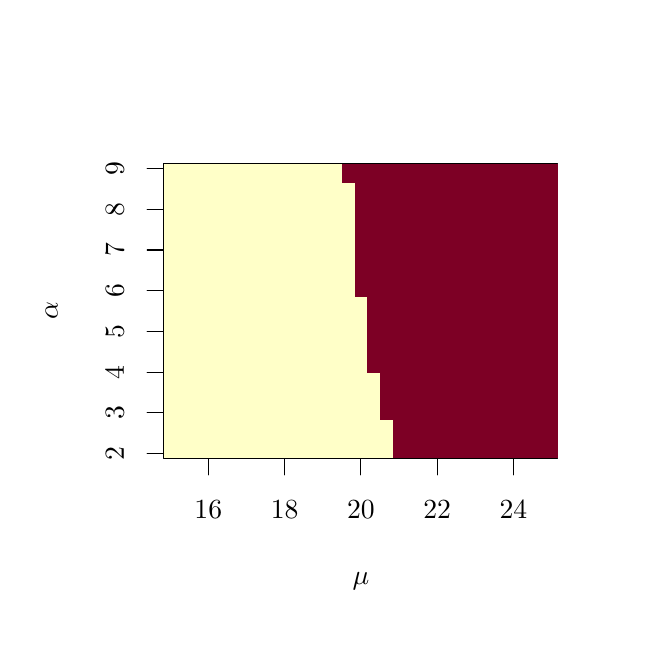
\begin{tikzpicture}[x=1pt,y=1pt]
\definecolor{fillColor}{RGB}{255,255,255}
\path[use as bounding box,fill=fillColor,fill opacity=0.00] (0,0) rectangle (216.81,216.81);
\begin{scope}
\path[clip] (  0.00,  0.00) rectangle (216.81,216.81);
\definecolor{drawColor}{RGB}{0,0,0}

\path[draw=drawColor,line width= 0.4pt,line join=round,line cap=round] ( 65.28, 61.20) -- (175.53, 61.20);

\path[draw=drawColor,line width= 0.4pt,line join=round,line cap=round] ( 65.28, 61.20) -- ( 65.28, 55.20);

\path[draw=drawColor,line width= 0.4pt,line join=round,line cap=round] ( 92.84, 61.20) -- ( 92.84, 55.20);

\path[draw=drawColor,line width= 0.4pt,line join=round,line cap=round] (120.40, 61.20) -- (120.40, 55.20);

\path[draw=drawColor,line width= 0.4pt,line join=round,line cap=round] (147.97, 61.20) -- (147.97, 55.20);

\path[draw=drawColor,line width= 0.4pt,line join=round,line cap=round] (175.53, 61.20) -- (175.53, 55.20);

\node[text=drawColor,anchor=base,inner sep=0pt, outer sep=0pt, scale=  1.00] at ( 65.28, 39.60) {16};

\node[text=drawColor,anchor=base,inner sep=0pt, outer sep=0pt, scale=  1.00] at ( 92.84, 39.60) {18};

\node[text=drawColor,anchor=base,inner sep=0pt, outer sep=0pt, scale=  1.00] at (120.40, 39.60) {20};

\node[text=drawColor,anchor=base,inner sep=0pt, outer sep=0pt, scale=  1.00] at (147.97, 39.60) {22};

\node[text=drawColor,anchor=base,inner sep=0pt, outer sep=0pt, scale=  1.00] at (175.53, 39.60) {24};

\path[draw=drawColor,line width= 0.4pt,line join=round,line cap=round] ( 49.20, 62.92) -- ( 49.20,165.89);

\path[draw=drawColor,line width= 0.4pt,line join=round,line cap=round] ( 49.20, 62.92) -- ( 43.20, 62.92);

\path[draw=drawColor,line width= 0.4pt,line join=round,line cap=round] ( 49.20, 77.63) -- ( 43.20, 77.63);

\path[draw=drawColor,line width= 0.4pt,line join=round,line cap=round] ( 49.20, 92.34) -- ( 43.20, 92.34);

\path[draw=drawColor,line width= 0.4pt,line join=round,line cap=round] ( 49.20,107.05) -- ( 43.20,107.05);

\path[draw=drawColor,line width= 0.4pt,line join=round,line cap=round] ( 49.20,121.76) -- ( 43.20,121.76);

\path[draw=drawColor,line width= 0.4pt,line join=round,line cap=round] ( 49.20,136.47) -- ( 43.20,136.47);

\path[draw=drawColor,line width= 0.4pt,line join=round,line cap=round] ( 49.20,151.18) -- ( 43.20,151.18);

\path[draw=drawColor,line width= 0.4pt,line join=round,line cap=round] ( 49.20,165.89) -- ( 43.20,165.89);

\node[text=drawColor,rotate= 90.00,anchor=base,inner sep=0pt, outer sep=0pt, scale=  1.00] at ( 34.80, 62.92) {2};

\node[text=drawColor,rotate= 90.00,anchor=base,inner sep=0pt, outer sep=0pt, scale=  1.00] at ( 34.80, 77.63) {3};

\node[text=drawColor,rotate= 90.00,anchor=base,inner sep=0pt, outer sep=0pt, scale=  1.00] at ( 34.80, 92.34) {4};

\node[text=drawColor,rotate= 90.00,anchor=base,inner sep=0pt, outer sep=0pt, scale=  1.00] at ( 34.80,107.05) {5};

\node[text=drawColor,rotate= 90.00,anchor=base,inner sep=0pt, outer sep=0pt, scale=  1.00] at ( 34.80,121.76) {6};

\node[text=drawColor,rotate= 90.00,anchor=base,inner sep=0pt, outer sep=0pt, scale=  1.00] at ( 34.80,136.47) {7};

\node[text=drawColor,rotate= 90.00,anchor=base,inner sep=0pt, outer sep=0pt, scale=  1.00] at ( 34.80,151.18) {8};

\node[text=drawColor,rotate= 90.00,anchor=base,inner sep=0pt, outer sep=0pt, scale=  1.00] at ( 34.80,165.89) {9};

\path[draw=drawColor,line width= 0.4pt,line join=round,line cap=round] ( 49.20, 61.20) --
	(191.61, 61.20) --
	(191.61,167.61) --
	( 49.20,167.61) --
	( 49.20, 61.20);
\end{scope}
\begin{scope}
\path[clip] (  0.00,  0.00) rectangle (216.81,216.81);
\definecolor{drawColor}{RGB}{0,0,0}

\node[text=drawColor,anchor=base,inner sep=0pt, outer sep=0pt, scale=  1.00] at (120.40, 15.60) {$\mu$};

\node[text=drawColor,rotate= 90.00,anchor=base,inner sep=0pt, outer sep=0pt, scale=  1.00] at ( 10.80,114.41) {$\alpha$};
\end{scope}
\begin{scope}
\path[clip] ( 49.20, 61.20) rectangle (191.61,167.61);
\definecolor{fillColor}{RGB}{255,255,200}

\path[fill=fillColor] ( 49.20, 61.20) rectangle ( 53.79, 64.63);

\path[fill=fillColor] ( 49.20, 64.63) rectangle ( 53.79, 68.07);

\path[fill=fillColor] ( 49.20, 68.07) rectangle ( 53.79, 71.50);

\path[fill=fillColor] ( 49.20, 71.50) rectangle ( 53.79, 74.93);

\path[fill=fillColor] ( 49.20, 74.93) rectangle ( 53.79, 78.36);

\path[fill=fillColor] ( 49.20, 78.36) rectangle ( 53.79, 81.80);

\path[fill=fillColor] ( 49.20, 81.80) rectangle ( 53.79, 85.23);

\path[fill=fillColor] ( 49.20, 85.23) rectangle ( 53.79, 88.66);

\path[fill=fillColor] ( 49.20, 88.66) rectangle ( 53.79, 92.09);

\path[fill=fillColor] ( 49.20, 92.09) rectangle ( 53.79, 95.53);

\path[fill=fillColor] ( 49.20, 95.53) rectangle ( 53.79, 98.96);

\path[fill=fillColor] ( 49.20, 98.96) rectangle ( 53.79,102.39);

\path[fill=fillColor] ( 49.20,102.39) rectangle ( 53.79,105.82);

\path[fill=fillColor] ( 49.20,105.82) rectangle ( 53.79,109.26);

\path[fill=fillColor] ( 49.20,109.26) rectangle ( 53.79,112.69);

\path[fill=fillColor] ( 49.20,112.69) rectangle ( 53.79,116.12);

\path[fill=fillColor] ( 49.20,116.12) rectangle ( 53.79,119.55);

\path[fill=fillColor] ( 49.20,119.55) rectangle ( 53.79,122.99);

\path[fill=fillColor] ( 49.20,122.99) rectangle ( 53.79,126.42);

\path[fill=fillColor] ( 49.20,126.42) rectangle ( 53.79,129.85);

\path[fill=fillColor] ( 49.20,129.85) rectangle ( 53.79,133.28);

\path[fill=fillColor] ( 49.20,133.28) rectangle ( 53.79,136.72);

\path[fill=fillColor] ( 49.20,136.72) rectangle ( 53.79,140.15);

\path[fill=fillColor] ( 49.20,140.15) rectangle ( 53.79,143.58);

\path[fill=fillColor] ( 49.20,143.58) rectangle ( 53.79,147.01);

\path[fill=fillColor] ( 49.20,147.01) rectangle ( 53.79,150.45);

\path[fill=fillColor] ( 49.20,150.45) rectangle ( 53.79,153.88);

\path[fill=fillColor] ( 49.20,153.88) rectangle ( 53.79,157.31);

\path[fill=fillColor] ( 49.20,157.31) rectangle ( 53.79,160.74);

\path[fill=fillColor] ( 49.20,160.74) rectangle ( 53.79,164.18);

\path[fill=fillColor] ( 49.20,164.18) rectangle ( 53.79,167.61);

\path[fill=fillColor] ( 53.79, 61.20) rectangle ( 58.39, 64.63);

\path[fill=fillColor] ( 53.79, 64.63) rectangle ( 58.39, 68.07);

\path[fill=fillColor] ( 53.79, 68.07) rectangle ( 58.39, 71.50);

\path[fill=fillColor] ( 53.79, 71.50) rectangle ( 58.39, 74.93);

\path[fill=fillColor] ( 53.79, 74.93) rectangle ( 58.39, 78.36);

\path[fill=fillColor] ( 53.79, 78.36) rectangle ( 58.39, 81.80);

\path[fill=fillColor] ( 53.79, 81.80) rectangle ( 58.39, 85.23);

\path[fill=fillColor] ( 53.79, 85.23) rectangle ( 58.39, 88.66);

\path[fill=fillColor] ( 53.79, 88.66) rectangle ( 58.39, 92.09);

\path[fill=fillColor] ( 53.79, 92.09) rectangle ( 58.39, 95.53);

\path[fill=fillColor] ( 53.79, 95.53) rectangle ( 58.39, 98.96);

\path[fill=fillColor] ( 53.79, 98.96) rectangle ( 58.39,102.39);

\path[fill=fillColor] ( 53.79,102.39) rectangle ( 58.39,105.82);

\path[fill=fillColor] ( 53.79,105.82) rectangle ( 58.39,109.26);

\path[fill=fillColor] ( 53.79,109.26) rectangle ( 58.39,112.69);

\path[fill=fillColor] ( 53.79,112.69) rectangle ( 58.39,116.12);

\path[fill=fillColor] ( 53.79,116.12) rectangle ( 58.39,119.55);

\path[fill=fillColor] ( 53.79,119.55) rectangle ( 58.39,122.99);

\path[fill=fillColor] ( 53.79,122.99) rectangle ( 58.39,126.42);

\path[fill=fillColor] ( 53.79,126.42) rectangle ( 58.39,129.85);

\path[fill=fillColor] ( 53.79,129.85) rectangle ( 58.39,133.28);

\path[fill=fillColor] ( 53.79,133.28) rectangle ( 58.39,136.72);

\path[fill=fillColor] ( 53.79,136.72) rectangle ( 58.39,140.15);

\path[fill=fillColor] ( 53.79,140.15) rectangle ( 58.39,143.58);

\path[fill=fillColor] ( 53.79,143.58) rectangle ( 58.39,147.01);

\path[fill=fillColor] ( 53.79,147.01) rectangle ( 58.39,150.45);

\path[fill=fillColor] ( 53.79,150.45) rectangle ( 58.39,153.88);

\path[fill=fillColor] ( 53.79,153.88) rectangle ( 58.39,157.31);

\path[fill=fillColor] ( 53.79,157.31) rectangle ( 58.39,160.74);

\path[fill=fillColor] ( 53.79,160.74) rectangle ( 58.39,164.18);

\path[fill=fillColor] ( 53.79,164.18) rectangle ( 58.39,167.61);

\path[fill=fillColor] ( 58.39, 61.20) rectangle ( 62.98, 64.63);

\path[fill=fillColor] ( 58.39, 64.63) rectangle ( 62.98, 68.07);

\path[fill=fillColor] ( 58.39, 68.07) rectangle ( 62.98, 71.50);

\path[fill=fillColor] ( 58.39, 71.50) rectangle ( 62.98, 74.93);

\path[fill=fillColor] ( 58.39, 74.93) rectangle ( 62.98, 78.36);

\path[fill=fillColor] ( 58.39, 78.36) rectangle ( 62.98, 81.80);

\path[fill=fillColor] ( 58.39, 81.80) rectangle ( 62.98, 85.23);

\path[fill=fillColor] ( 58.39, 85.23) rectangle ( 62.98, 88.66);

\path[fill=fillColor] ( 58.39, 88.66) rectangle ( 62.98, 92.09);

\path[fill=fillColor] ( 58.39, 92.09) rectangle ( 62.98, 95.53);

\path[fill=fillColor] ( 58.39, 95.53) rectangle ( 62.98, 98.96);

\path[fill=fillColor] ( 58.39, 98.96) rectangle ( 62.98,102.39);

\path[fill=fillColor] ( 58.39,102.39) rectangle ( 62.98,105.82);

\path[fill=fillColor] ( 58.39,105.82) rectangle ( 62.98,109.26);

\path[fill=fillColor] ( 58.39,109.26) rectangle ( 62.98,112.69);

\path[fill=fillColor] ( 58.39,112.69) rectangle ( 62.98,116.12);

\path[fill=fillColor] ( 58.39,116.12) rectangle ( 62.98,119.55);

\path[fill=fillColor] ( 58.39,119.55) rectangle ( 62.98,122.99);

\path[fill=fillColor] ( 58.39,122.99) rectangle ( 62.98,126.42);

\path[fill=fillColor] ( 58.39,126.42) rectangle ( 62.98,129.85);

\path[fill=fillColor] ( 58.39,129.85) rectangle ( 62.98,133.28);

\path[fill=fillColor] ( 58.39,133.28) rectangle ( 62.98,136.72);

\path[fill=fillColor] ( 58.39,136.72) rectangle ( 62.98,140.15);

\path[fill=fillColor] ( 58.39,140.15) rectangle ( 62.98,143.58);

\path[fill=fillColor] ( 58.39,143.58) rectangle ( 62.98,147.01);

\path[fill=fillColor] ( 58.39,147.01) rectangle ( 62.98,150.45);

\path[fill=fillColor] ( 58.39,150.45) rectangle ( 62.98,153.88);

\path[fill=fillColor] ( 58.39,153.88) rectangle ( 62.98,157.31);

\path[fill=fillColor] ( 58.39,157.31) rectangle ( 62.98,160.74);

\path[fill=fillColor] ( 58.39,160.74) rectangle ( 62.98,164.18);

\path[fill=fillColor] ( 58.39,164.18) rectangle ( 62.98,167.61);

\path[fill=fillColor] ( 62.98, 61.20) rectangle ( 67.58, 64.63);

\path[fill=fillColor] ( 62.98, 64.63) rectangle ( 67.58, 68.07);

\path[fill=fillColor] ( 62.98, 68.07) rectangle ( 67.58, 71.50);

\path[fill=fillColor] ( 62.98, 71.50) rectangle ( 67.58, 74.93);

\path[fill=fillColor] ( 62.98, 74.93) rectangle ( 67.58, 78.36);

\path[fill=fillColor] ( 62.98, 78.36) rectangle ( 67.58, 81.80);

\path[fill=fillColor] ( 62.98, 81.80) rectangle ( 67.58, 85.23);

\path[fill=fillColor] ( 62.98, 85.23) rectangle ( 67.58, 88.66);

\path[fill=fillColor] ( 62.98, 88.66) rectangle ( 67.58, 92.09);

\path[fill=fillColor] ( 62.98, 92.09) rectangle ( 67.58, 95.53);

\path[fill=fillColor] ( 62.98, 95.53) rectangle ( 67.58, 98.96);

\path[fill=fillColor] ( 62.98, 98.96) rectangle ( 67.58,102.39);

\path[fill=fillColor] ( 62.98,102.39) rectangle ( 67.58,105.82);

\path[fill=fillColor] ( 62.98,105.82) rectangle ( 67.58,109.26);

\path[fill=fillColor] ( 62.98,109.26) rectangle ( 67.58,112.69);

\path[fill=fillColor] ( 62.98,112.69) rectangle ( 67.58,116.12);

\path[fill=fillColor] ( 62.98,116.12) rectangle ( 67.58,119.55);

\path[fill=fillColor] ( 62.98,119.55) rectangle ( 67.58,122.99);

\path[fill=fillColor] ( 62.98,122.99) rectangle ( 67.58,126.42);

\path[fill=fillColor] ( 62.98,126.42) rectangle ( 67.58,129.85);

\path[fill=fillColor] ( 62.98,129.85) rectangle ( 67.58,133.28);

\path[fill=fillColor] ( 62.98,133.28) rectangle ( 67.58,136.72);

\path[fill=fillColor] ( 62.98,136.72) rectangle ( 67.58,140.15);

\path[fill=fillColor] ( 62.98,140.15) rectangle ( 67.58,143.58);

\path[fill=fillColor] ( 62.98,143.58) rectangle ( 67.58,147.01);

\path[fill=fillColor] ( 62.98,147.01) rectangle ( 67.58,150.45);

\path[fill=fillColor] ( 62.98,150.45) rectangle ( 67.58,153.88);

\path[fill=fillColor] ( 62.98,153.88) rectangle ( 67.58,157.31);

\path[fill=fillColor] ( 62.98,157.31) rectangle ( 67.58,160.74);

\path[fill=fillColor] ( 62.98,160.74) rectangle ( 67.58,164.18);

\path[fill=fillColor] ( 62.98,164.18) rectangle ( 67.58,167.61);

\path[fill=fillColor] ( 67.58, 61.20) rectangle ( 72.17, 64.63);

\path[fill=fillColor] ( 67.58, 64.63) rectangle ( 72.17, 68.07);

\path[fill=fillColor] ( 67.58, 68.07) rectangle ( 72.17, 71.50);

\path[fill=fillColor] ( 67.58, 71.50) rectangle ( 72.17, 74.93);

\path[fill=fillColor] ( 67.58, 74.93) rectangle ( 72.17, 78.36);

\path[fill=fillColor] ( 67.58, 78.36) rectangle ( 72.17, 81.80);

\path[fill=fillColor] ( 67.58, 81.80) rectangle ( 72.17, 85.23);

\path[fill=fillColor] ( 67.58, 85.23) rectangle ( 72.17, 88.66);

\path[fill=fillColor] ( 67.58, 88.66) rectangle ( 72.17, 92.09);

\path[fill=fillColor] ( 67.58, 92.09) rectangle ( 72.17, 95.53);

\path[fill=fillColor] ( 67.58, 95.53) rectangle ( 72.17, 98.96);

\path[fill=fillColor] ( 67.58, 98.96) rectangle ( 72.17,102.39);

\path[fill=fillColor] ( 67.58,102.39) rectangle ( 72.17,105.82);

\path[fill=fillColor] ( 67.58,105.82) rectangle ( 72.17,109.26);

\path[fill=fillColor] ( 67.58,109.26) rectangle ( 72.17,112.69);

\path[fill=fillColor] ( 67.58,112.69) rectangle ( 72.17,116.12);

\path[fill=fillColor] ( 67.58,116.12) rectangle ( 72.17,119.55);

\path[fill=fillColor] ( 67.58,119.55) rectangle ( 72.17,122.99);

\path[fill=fillColor] ( 67.58,122.99) rectangle ( 72.17,126.42);

\path[fill=fillColor] ( 67.58,126.42) rectangle ( 72.17,129.85);

\path[fill=fillColor] ( 67.58,129.85) rectangle ( 72.17,133.28);

\path[fill=fillColor] ( 67.58,133.28) rectangle ( 72.17,136.72);

\path[fill=fillColor] ( 67.58,136.72) rectangle ( 72.17,140.15);

\path[fill=fillColor] ( 67.58,140.15) rectangle ( 72.17,143.58);

\path[fill=fillColor] ( 67.58,143.58) rectangle ( 72.17,147.01);

\path[fill=fillColor] ( 67.58,147.01) rectangle ( 72.17,150.45);

\path[fill=fillColor] ( 67.58,150.45) rectangle ( 72.17,153.88);

\path[fill=fillColor] ( 67.58,153.88) rectangle ( 72.17,157.31);

\path[fill=fillColor] ( 67.58,157.31) rectangle ( 72.17,160.74);

\path[fill=fillColor] ( 67.58,160.74) rectangle ( 72.17,164.18);

\path[fill=fillColor] ( 67.58,164.18) rectangle ( 72.17,167.61);

\path[fill=fillColor] ( 72.17, 61.20) rectangle ( 76.76, 64.63);

\path[fill=fillColor] ( 72.17, 64.63) rectangle ( 76.76, 68.07);

\path[fill=fillColor] ( 72.17, 68.07) rectangle ( 76.76, 71.50);

\path[fill=fillColor] ( 72.17, 71.50) rectangle ( 76.76, 74.93);

\path[fill=fillColor] ( 72.17, 74.93) rectangle ( 76.76, 78.36);

\path[fill=fillColor] ( 72.17, 78.36) rectangle ( 76.76, 81.80);

\path[fill=fillColor] ( 72.17, 81.80) rectangle ( 76.76, 85.23);

\path[fill=fillColor] ( 72.17, 85.23) rectangle ( 76.76, 88.66);

\path[fill=fillColor] ( 72.17, 88.66) rectangle ( 76.76, 92.09);

\path[fill=fillColor] ( 72.17, 92.09) rectangle ( 76.76, 95.53);

\path[fill=fillColor] ( 72.17, 95.53) rectangle ( 76.76, 98.96);

\path[fill=fillColor] ( 72.17, 98.96) rectangle ( 76.76,102.39);

\path[fill=fillColor] ( 72.17,102.39) rectangle ( 76.76,105.82);

\path[fill=fillColor] ( 72.17,105.82) rectangle ( 76.76,109.26);

\path[fill=fillColor] ( 72.17,109.26) rectangle ( 76.76,112.69);

\path[fill=fillColor] ( 72.17,112.69) rectangle ( 76.76,116.12);

\path[fill=fillColor] ( 72.17,116.12) rectangle ( 76.76,119.55);

\path[fill=fillColor] ( 72.17,119.55) rectangle ( 76.76,122.99);

\path[fill=fillColor] ( 72.17,122.99) rectangle ( 76.76,126.42);

\path[fill=fillColor] ( 72.17,126.42) rectangle ( 76.76,129.85);

\path[fill=fillColor] ( 72.17,129.85) rectangle ( 76.76,133.28);

\path[fill=fillColor] ( 72.17,133.28) rectangle ( 76.76,136.72);

\path[fill=fillColor] ( 72.17,136.72) rectangle ( 76.76,140.15);

\path[fill=fillColor] ( 72.17,140.15) rectangle ( 76.76,143.58);

\path[fill=fillColor] ( 72.17,143.58) rectangle ( 76.76,147.01);

\path[fill=fillColor] ( 72.17,147.01) rectangle ( 76.76,150.45);

\path[fill=fillColor] ( 72.17,150.45) rectangle ( 76.76,153.88);

\path[fill=fillColor] ( 72.17,153.88) rectangle ( 76.76,157.31);

\path[fill=fillColor] ( 72.17,157.31) rectangle ( 76.76,160.74);

\path[fill=fillColor] ( 72.17,160.74) rectangle ( 76.76,164.18);

\path[fill=fillColor] ( 72.17,164.18) rectangle ( 76.76,167.61);

\path[fill=fillColor] ( 76.76, 61.20) rectangle ( 81.36, 64.63);

\path[fill=fillColor] ( 76.76, 64.63) rectangle ( 81.36, 68.07);

\path[fill=fillColor] ( 76.76, 68.07) rectangle ( 81.36, 71.50);

\path[fill=fillColor] ( 76.76, 71.50) rectangle ( 81.36, 74.93);

\path[fill=fillColor] ( 76.76, 74.93) rectangle ( 81.36, 78.36);

\path[fill=fillColor] ( 76.76, 78.36) rectangle ( 81.36, 81.80);

\path[fill=fillColor] ( 76.76, 81.80) rectangle ( 81.36, 85.23);

\path[fill=fillColor] ( 76.76, 85.23) rectangle ( 81.36, 88.66);

\path[fill=fillColor] ( 76.76, 88.66) rectangle ( 81.36, 92.09);

\path[fill=fillColor] ( 76.76, 92.09) rectangle ( 81.36, 95.53);

\path[fill=fillColor] ( 76.76, 95.53) rectangle ( 81.36, 98.96);

\path[fill=fillColor] ( 76.76, 98.96) rectangle ( 81.36,102.39);

\path[fill=fillColor] ( 76.76,102.39) rectangle ( 81.36,105.82);

\path[fill=fillColor] ( 76.76,105.82) rectangle ( 81.36,109.26);

\path[fill=fillColor] ( 76.76,109.26) rectangle ( 81.36,112.69);

\path[fill=fillColor] ( 76.76,112.69) rectangle ( 81.36,116.12);

\path[fill=fillColor] ( 76.76,116.12) rectangle ( 81.36,119.55);

\path[fill=fillColor] ( 76.76,119.55) rectangle ( 81.36,122.99);

\path[fill=fillColor] ( 76.76,122.99) rectangle ( 81.36,126.42);

\path[fill=fillColor] ( 76.76,126.42) rectangle ( 81.36,129.85);

\path[fill=fillColor] ( 76.76,129.85) rectangle ( 81.36,133.28);

\path[fill=fillColor] ( 76.76,133.28) rectangle ( 81.36,136.72);

\path[fill=fillColor] ( 76.76,136.72) rectangle ( 81.36,140.15);

\path[fill=fillColor] ( 76.76,140.15) rectangle ( 81.36,143.58);

\path[fill=fillColor] ( 76.76,143.58) rectangle ( 81.36,147.01);

\path[fill=fillColor] ( 76.76,147.01) rectangle ( 81.36,150.45);

\path[fill=fillColor] ( 76.76,150.45) rectangle ( 81.36,153.88);

\path[fill=fillColor] ( 76.76,153.88) rectangle ( 81.36,157.31);

\path[fill=fillColor] ( 76.76,157.31) rectangle ( 81.36,160.74);

\path[fill=fillColor] ( 76.76,160.74) rectangle ( 81.36,164.18);

\path[fill=fillColor] ( 76.76,164.18) rectangle ( 81.36,167.61);

\path[fill=fillColor] ( 81.36, 61.20) rectangle ( 85.95, 64.63);

\path[fill=fillColor] ( 81.36, 64.63) rectangle ( 85.95, 68.07);

\path[fill=fillColor] ( 81.36, 68.07) rectangle ( 85.95, 71.50);

\path[fill=fillColor] ( 81.36, 71.50) rectangle ( 85.95, 74.93);

\path[fill=fillColor] ( 81.36, 74.93) rectangle ( 85.95, 78.36);

\path[fill=fillColor] ( 81.36, 78.36) rectangle ( 85.95, 81.80);

\path[fill=fillColor] ( 81.36, 81.80) rectangle ( 85.95, 85.23);

\path[fill=fillColor] ( 81.36, 85.23) rectangle ( 85.95, 88.66);

\path[fill=fillColor] ( 81.36, 88.66) rectangle ( 85.95, 92.09);

\path[fill=fillColor] ( 81.36, 92.09) rectangle ( 85.95, 95.53);

\path[fill=fillColor] ( 81.36, 95.53) rectangle ( 85.95, 98.96);

\path[fill=fillColor] ( 81.36, 98.96) rectangle ( 85.95,102.39);

\path[fill=fillColor] ( 81.36,102.39) rectangle ( 85.95,105.82);

\path[fill=fillColor] ( 81.36,105.82) rectangle ( 85.95,109.26);

\path[fill=fillColor] ( 81.36,109.26) rectangle ( 85.95,112.69);

\path[fill=fillColor] ( 81.36,112.69) rectangle ( 85.95,116.12);

\path[fill=fillColor] ( 81.36,116.12) rectangle ( 85.95,119.55);

\path[fill=fillColor] ( 81.36,119.55) rectangle ( 85.95,122.99);

\path[fill=fillColor] ( 81.36,122.99) rectangle ( 85.95,126.42);

\path[fill=fillColor] ( 81.36,126.42) rectangle ( 85.95,129.85);

\path[fill=fillColor] ( 81.36,129.85) rectangle ( 85.95,133.28);

\path[fill=fillColor] ( 81.36,133.28) rectangle ( 85.95,136.72);

\path[fill=fillColor] ( 81.36,136.72) rectangle ( 85.95,140.15);

\path[fill=fillColor] ( 81.36,140.15) rectangle ( 85.95,143.58);

\path[fill=fillColor] ( 81.36,143.58) rectangle ( 85.95,147.01);

\path[fill=fillColor] ( 81.36,147.01) rectangle ( 85.95,150.45);

\path[fill=fillColor] ( 81.36,150.45) rectangle ( 85.95,153.88);

\path[fill=fillColor] ( 81.36,153.88) rectangle ( 85.95,157.31);

\path[fill=fillColor] ( 81.36,157.31) rectangle ( 85.95,160.74);

\path[fill=fillColor] ( 81.36,160.74) rectangle ( 85.95,164.18);

\path[fill=fillColor] ( 81.36,164.18) rectangle ( 85.95,167.61);

\path[fill=fillColor] ( 85.95, 61.20) rectangle ( 90.54, 64.63);

\path[fill=fillColor] ( 85.95, 64.63) rectangle ( 90.54, 68.07);

\path[fill=fillColor] ( 85.95, 68.07) rectangle ( 90.54, 71.50);

\path[fill=fillColor] ( 85.95, 71.50) rectangle ( 90.54, 74.93);

\path[fill=fillColor] ( 85.95, 74.93) rectangle ( 90.54, 78.36);

\path[fill=fillColor] ( 85.95, 78.36) rectangle ( 90.54, 81.80);

\path[fill=fillColor] ( 85.95, 81.80) rectangle ( 90.54, 85.23);

\path[fill=fillColor] ( 85.95, 85.23) rectangle ( 90.54, 88.66);

\path[fill=fillColor] ( 85.95, 88.66) rectangle ( 90.54, 92.09);

\path[fill=fillColor] ( 85.95, 92.09) rectangle ( 90.54, 95.53);

\path[fill=fillColor] ( 85.95, 95.53) rectangle ( 90.54, 98.96);

\path[fill=fillColor] ( 85.95, 98.96) rectangle ( 90.54,102.39);

\path[fill=fillColor] ( 85.95,102.39) rectangle ( 90.54,105.82);

\path[fill=fillColor] ( 85.95,105.82) rectangle ( 90.54,109.26);

\path[fill=fillColor] ( 85.95,109.26) rectangle ( 90.54,112.69);

\path[fill=fillColor] ( 85.95,112.69) rectangle ( 90.54,116.12);

\path[fill=fillColor] ( 85.95,116.12) rectangle ( 90.54,119.55);

\path[fill=fillColor] ( 85.95,119.55) rectangle ( 90.54,122.99);

\path[fill=fillColor] ( 85.95,122.99) rectangle ( 90.54,126.42);

\path[fill=fillColor] ( 85.95,126.42) rectangle ( 90.54,129.85);

\path[fill=fillColor] ( 85.95,129.85) rectangle ( 90.54,133.28);

\path[fill=fillColor] ( 85.95,133.28) rectangle ( 90.54,136.72);

\path[fill=fillColor] ( 85.95,136.72) rectangle ( 90.54,140.15);

\path[fill=fillColor] ( 85.95,140.15) rectangle ( 90.54,143.58);

\path[fill=fillColor] ( 85.95,143.58) rectangle ( 90.54,147.01);

\path[fill=fillColor] ( 85.95,147.01) rectangle ( 90.54,150.45);

\path[fill=fillColor] ( 85.95,150.45) rectangle ( 90.54,153.88);

\path[fill=fillColor] ( 85.95,153.88) rectangle ( 90.54,157.31);

\path[fill=fillColor] ( 85.95,157.31) rectangle ( 90.54,160.74);

\path[fill=fillColor] ( 85.95,160.74) rectangle ( 90.54,164.18);

\path[fill=fillColor] ( 85.95,164.18) rectangle ( 90.54,167.61);

\path[fill=fillColor] ( 90.54, 61.20) rectangle ( 95.14, 64.63);

\path[fill=fillColor] ( 90.54, 64.63) rectangle ( 95.14, 68.07);

\path[fill=fillColor] ( 90.54, 68.07) rectangle ( 95.14, 71.50);

\path[fill=fillColor] ( 90.54, 71.50) rectangle ( 95.14, 74.93);

\path[fill=fillColor] ( 90.54, 74.93) rectangle ( 95.14, 78.36);

\path[fill=fillColor] ( 90.54, 78.36) rectangle ( 95.14, 81.80);

\path[fill=fillColor] ( 90.54, 81.80) rectangle ( 95.14, 85.23);

\path[fill=fillColor] ( 90.54, 85.23) rectangle ( 95.14, 88.66);

\path[fill=fillColor] ( 90.54, 88.66) rectangle ( 95.14, 92.09);

\path[fill=fillColor] ( 90.54, 92.09) rectangle ( 95.14, 95.53);

\path[fill=fillColor] ( 90.54, 95.53) rectangle ( 95.14, 98.96);

\path[fill=fillColor] ( 90.54, 98.96) rectangle ( 95.14,102.39);

\path[fill=fillColor] ( 90.54,102.39) rectangle ( 95.14,105.82);

\path[fill=fillColor] ( 90.54,105.82) rectangle ( 95.14,109.26);

\path[fill=fillColor] ( 90.54,109.26) rectangle ( 95.14,112.69);

\path[fill=fillColor] ( 90.54,112.69) rectangle ( 95.14,116.12);

\path[fill=fillColor] ( 90.54,116.12) rectangle ( 95.14,119.55);

\path[fill=fillColor] ( 90.54,119.55) rectangle ( 95.14,122.99);

\path[fill=fillColor] ( 90.54,122.99) rectangle ( 95.14,126.42);

\path[fill=fillColor] ( 90.54,126.42) rectangle ( 95.14,129.85);

\path[fill=fillColor] ( 90.54,129.85) rectangle ( 95.14,133.28);

\path[fill=fillColor] ( 90.54,133.28) rectangle ( 95.14,136.72);

\path[fill=fillColor] ( 90.54,136.72) rectangle ( 95.14,140.15);

\path[fill=fillColor] ( 90.54,140.15) rectangle ( 95.14,143.58);

\path[fill=fillColor] ( 90.54,143.58) rectangle ( 95.14,147.01);

\path[fill=fillColor] ( 90.54,147.01) rectangle ( 95.14,150.45);

\path[fill=fillColor] ( 90.54,150.45) rectangle ( 95.14,153.88);

\path[fill=fillColor] ( 90.54,153.88) rectangle ( 95.14,157.31);

\path[fill=fillColor] ( 90.54,157.31) rectangle ( 95.14,160.74);

\path[fill=fillColor] ( 90.54,160.74) rectangle ( 95.14,164.18);

\path[fill=fillColor] ( 90.54,164.18) rectangle ( 95.14,167.61);

\path[fill=fillColor] ( 95.14, 61.20) rectangle ( 99.73, 64.63);

\path[fill=fillColor] ( 95.14, 64.63) rectangle ( 99.73, 68.07);

\path[fill=fillColor] ( 95.14, 68.07) rectangle ( 99.73, 71.50);

\path[fill=fillColor] ( 95.14, 71.50) rectangle ( 99.73, 74.93);

\path[fill=fillColor] ( 95.14, 74.93) rectangle ( 99.73, 78.36);

\path[fill=fillColor] ( 95.14, 78.36) rectangle ( 99.73, 81.80);

\path[fill=fillColor] ( 95.14, 81.80) rectangle ( 99.73, 85.23);

\path[fill=fillColor] ( 95.14, 85.23) rectangle ( 99.73, 88.66);

\path[fill=fillColor] ( 95.14, 88.66) rectangle ( 99.73, 92.09);

\path[fill=fillColor] ( 95.14, 92.09) rectangle ( 99.73, 95.53);

\path[fill=fillColor] ( 95.14, 95.53) rectangle ( 99.73, 98.96);

\path[fill=fillColor] ( 95.14, 98.96) rectangle ( 99.73,102.39);

\path[fill=fillColor] ( 95.14,102.39) rectangle ( 99.73,105.82);

\path[fill=fillColor] ( 95.14,105.82) rectangle ( 99.73,109.26);

\path[fill=fillColor] ( 95.14,109.26) rectangle ( 99.73,112.69);

\path[fill=fillColor] ( 95.14,112.69) rectangle ( 99.73,116.12);

\path[fill=fillColor] ( 95.14,116.12) rectangle ( 99.73,119.55);

\path[fill=fillColor] ( 95.14,119.55) rectangle ( 99.73,122.99);

\path[fill=fillColor] ( 95.14,122.99) rectangle ( 99.73,126.42);

\path[fill=fillColor] ( 95.14,126.42) rectangle ( 99.73,129.85);

\path[fill=fillColor] ( 95.14,129.85) rectangle ( 99.73,133.28);

\path[fill=fillColor] ( 95.14,133.28) rectangle ( 99.73,136.72);

\path[fill=fillColor] ( 95.14,136.72) rectangle ( 99.73,140.15);

\path[fill=fillColor] ( 95.14,140.15) rectangle ( 99.73,143.58);

\path[fill=fillColor] ( 95.14,143.58) rectangle ( 99.73,147.01);

\path[fill=fillColor] ( 95.14,147.01) rectangle ( 99.73,150.45);

\path[fill=fillColor] ( 95.14,150.45) rectangle ( 99.73,153.88);

\path[fill=fillColor] ( 95.14,153.88) rectangle ( 99.73,157.31);

\path[fill=fillColor] ( 95.14,157.31) rectangle ( 99.73,160.74);

\path[fill=fillColor] ( 95.14,160.74) rectangle ( 99.73,164.18);

\path[fill=fillColor] ( 95.14,164.18) rectangle ( 99.73,167.61);

\path[fill=fillColor] ( 99.73, 61.20) rectangle (104.33, 64.63);

\path[fill=fillColor] ( 99.73, 64.63) rectangle (104.33, 68.07);

\path[fill=fillColor] ( 99.73, 68.07) rectangle (104.33, 71.50);

\path[fill=fillColor] ( 99.73, 71.50) rectangle (104.33, 74.93);

\path[fill=fillColor] ( 99.73, 74.93) rectangle (104.33, 78.36);

\path[fill=fillColor] ( 99.73, 78.36) rectangle (104.33, 81.80);

\path[fill=fillColor] ( 99.73, 81.80) rectangle (104.33, 85.23);

\path[fill=fillColor] ( 99.73, 85.23) rectangle (104.33, 88.66);

\path[fill=fillColor] ( 99.73, 88.66) rectangle (104.33, 92.09);

\path[fill=fillColor] ( 99.73, 92.09) rectangle (104.33, 95.53);

\path[fill=fillColor] ( 99.73, 95.53) rectangle (104.33, 98.96);

\path[fill=fillColor] ( 99.73, 98.96) rectangle (104.33,102.39);

\path[fill=fillColor] ( 99.73,102.39) rectangle (104.33,105.82);

\path[fill=fillColor] ( 99.73,105.82) rectangle (104.33,109.26);

\path[fill=fillColor] ( 99.73,109.26) rectangle (104.33,112.69);

\path[fill=fillColor] ( 99.73,112.69) rectangle (104.33,116.12);

\path[fill=fillColor] ( 99.73,116.12) rectangle (104.33,119.55);

\path[fill=fillColor] ( 99.73,119.55) rectangle (104.33,122.99);

\path[fill=fillColor] ( 99.73,122.99) rectangle (104.33,126.42);

\path[fill=fillColor] ( 99.73,126.42) rectangle (104.33,129.85);

\path[fill=fillColor] ( 99.73,129.85) rectangle (104.33,133.28);

\path[fill=fillColor] ( 99.73,133.28) rectangle (104.33,136.72);

\path[fill=fillColor] ( 99.73,136.72) rectangle (104.33,140.15);

\path[fill=fillColor] ( 99.73,140.15) rectangle (104.33,143.58);

\path[fill=fillColor] ( 99.73,143.58) rectangle (104.33,147.01);

\path[fill=fillColor] ( 99.73,147.01) rectangle (104.33,150.45);

\path[fill=fillColor] ( 99.73,150.45) rectangle (104.33,153.88);

\path[fill=fillColor] ( 99.73,153.88) rectangle (104.33,157.31);

\path[fill=fillColor] ( 99.73,157.31) rectangle (104.33,160.74);

\path[fill=fillColor] ( 99.73,160.74) rectangle (104.33,164.18);

\path[fill=fillColor] ( 99.73,164.18) rectangle (104.33,167.61);

\path[fill=fillColor] (104.33, 61.20) rectangle (108.92, 64.63);

\path[fill=fillColor] (104.33, 64.63) rectangle (108.92, 68.07);

\path[fill=fillColor] (104.33, 68.07) rectangle (108.92, 71.50);

\path[fill=fillColor] (104.33, 71.50) rectangle (108.92, 74.93);

\path[fill=fillColor] (104.33, 74.93) rectangle (108.92, 78.36);

\path[fill=fillColor] (104.33, 78.36) rectangle (108.92, 81.80);

\path[fill=fillColor] (104.33, 81.80) rectangle (108.92, 85.23);

\path[fill=fillColor] (104.33, 85.23) rectangle (108.92, 88.66);

\path[fill=fillColor] (104.33, 88.66) rectangle (108.92, 92.09);

\path[fill=fillColor] (104.33, 92.09) rectangle (108.92, 95.53);

\path[fill=fillColor] (104.33, 95.53) rectangle (108.92, 98.96);

\path[fill=fillColor] (104.33, 98.96) rectangle (108.92,102.39);

\path[fill=fillColor] (104.33,102.39) rectangle (108.92,105.82);

\path[fill=fillColor] (104.33,105.82) rectangle (108.92,109.26);

\path[fill=fillColor] (104.33,109.26) rectangle (108.92,112.69);

\path[fill=fillColor] (104.33,112.69) rectangle (108.92,116.12);

\path[fill=fillColor] (104.33,116.12) rectangle (108.92,119.55);

\path[fill=fillColor] (104.33,119.55) rectangle (108.92,122.99);

\path[fill=fillColor] (104.33,122.99) rectangle (108.92,126.42);

\path[fill=fillColor] (104.33,126.42) rectangle (108.92,129.85);

\path[fill=fillColor] (104.33,129.85) rectangle (108.92,133.28);

\path[fill=fillColor] (104.33,133.28) rectangle (108.92,136.72);

\path[fill=fillColor] (104.33,136.72) rectangle (108.92,140.15);

\path[fill=fillColor] (104.33,140.15) rectangle (108.92,143.58);

\path[fill=fillColor] (104.33,143.58) rectangle (108.92,147.01);

\path[fill=fillColor] (104.33,147.01) rectangle (108.92,150.45);

\path[fill=fillColor] (104.33,150.45) rectangle (108.92,153.88);

\path[fill=fillColor] (104.33,153.88) rectangle (108.92,157.31);

\path[fill=fillColor] (104.33,157.31) rectangle (108.92,160.74);

\path[fill=fillColor] (104.33,160.74) rectangle (108.92,164.18);

\path[fill=fillColor] (104.33,164.18) rectangle (108.92,167.61);

\path[fill=fillColor] (108.92, 61.20) rectangle (113.51, 64.63);

\path[fill=fillColor] (108.92, 64.63) rectangle (113.51, 68.07);

\path[fill=fillColor] (108.92, 68.07) rectangle (113.51, 71.50);

\path[fill=fillColor] (108.92, 71.50) rectangle (113.51, 74.93);

\path[fill=fillColor] (108.92, 74.93) rectangle (113.51, 78.36);

\path[fill=fillColor] (108.92, 78.36) rectangle (113.51, 81.80);

\path[fill=fillColor] (108.92, 81.80) rectangle (113.51, 85.23);

\path[fill=fillColor] (108.92, 85.23) rectangle (113.51, 88.66);

\path[fill=fillColor] (108.92, 88.66) rectangle (113.51, 92.09);

\path[fill=fillColor] (108.92, 92.09) rectangle (113.51, 95.53);

\path[fill=fillColor] (108.92, 95.53) rectangle (113.51, 98.96);

\path[fill=fillColor] (108.92, 98.96) rectangle (113.51,102.39);

\path[fill=fillColor] (108.92,102.39) rectangle (113.51,105.82);

\path[fill=fillColor] (108.92,105.82) rectangle (113.51,109.26);

\path[fill=fillColor] (108.92,109.26) rectangle (113.51,112.69);

\path[fill=fillColor] (108.92,112.69) rectangle (113.51,116.12);

\path[fill=fillColor] (108.92,116.12) rectangle (113.51,119.55);

\path[fill=fillColor] (108.92,119.55) rectangle (113.51,122.99);

\path[fill=fillColor] (108.92,122.99) rectangle (113.51,126.42);

\path[fill=fillColor] (108.92,126.42) rectangle (113.51,129.85);

\path[fill=fillColor] (108.92,129.85) rectangle (113.51,133.28);

\path[fill=fillColor] (108.92,133.28) rectangle (113.51,136.72);

\path[fill=fillColor] (108.92,136.72) rectangle (113.51,140.15);

\path[fill=fillColor] (108.92,140.15) rectangle (113.51,143.58);

\path[fill=fillColor] (108.92,143.58) rectangle (113.51,147.01);

\path[fill=fillColor] (108.92,147.01) rectangle (113.51,150.45);

\path[fill=fillColor] (108.92,150.45) rectangle (113.51,153.88);

\path[fill=fillColor] (108.92,153.88) rectangle (113.51,157.31);

\path[fill=fillColor] (108.92,157.31) rectangle (113.51,160.74);

\path[fill=fillColor] (108.92,160.74) rectangle (113.51,164.18);

\path[fill=fillColor] (108.92,164.18) rectangle (113.51,167.61);

\path[fill=fillColor] (113.51, 61.20) rectangle (118.11, 64.63);

\path[fill=fillColor] (113.51, 64.63) rectangle (118.11, 68.07);

\path[fill=fillColor] (113.51, 68.07) rectangle (118.11, 71.50);

\path[fill=fillColor] (113.51, 71.50) rectangle (118.11, 74.93);

\path[fill=fillColor] (113.51, 74.93) rectangle (118.11, 78.36);

\path[fill=fillColor] (113.51, 78.36) rectangle (118.11, 81.80);

\path[fill=fillColor] (113.51, 81.80) rectangle (118.11, 85.23);

\path[fill=fillColor] (113.51, 85.23) rectangle (118.11, 88.66);

\path[fill=fillColor] (113.51, 88.66) rectangle (118.11, 92.09);

\path[fill=fillColor] (113.51, 92.09) rectangle (118.11, 95.53);

\path[fill=fillColor] (113.51, 95.53) rectangle (118.11, 98.96);

\path[fill=fillColor] (113.51, 98.96) rectangle (118.11,102.39);

\path[fill=fillColor] (113.51,102.39) rectangle (118.11,105.82);

\path[fill=fillColor] (113.51,105.82) rectangle (118.11,109.26);

\path[fill=fillColor] (113.51,109.26) rectangle (118.11,112.69);

\path[fill=fillColor] (113.51,112.69) rectangle (118.11,116.12);

\path[fill=fillColor] (113.51,116.12) rectangle (118.11,119.55);

\path[fill=fillColor] (113.51,119.55) rectangle (118.11,122.99);

\path[fill=fillColor] (113.51,122.99) rectangle (118.11,126.42);

\path[fill=fillColor] (113.51,126.42) rectangle (118.11,129.85);

\path[fill=fillColor] (113.51,129.85) rectangle (118.11,133.28);

\path[fill=fillColor] (113.51,133.28) rectangle (118.11,136.72);

\path[fill=fillColor] (113.51,136.72) rectangle (118.11,140.15);

\path[fill=fillColor] (113.51,140.15) rectangle (118.11,143.58);

\path[fill=fillColor] (113.51,143.58) rectangle (118.11,147.01);

\path[fill=fillColor] (113.51,147.01) rectangle (118.11,150.45);

\path[fill=fillColor] (113.51,150.45) rectangle (118.11,153.88);

\path[fill=fillColor] (113.51,153.88) rectangle (118.11,157.31);

\path[fill=fillColor] (113.51,157.31) rectangle (118.11,160.74);
\definecolor{fillColor}{RGB}{125,0,37}

\path[fill=fillColor] (113.51,160.74) rectangle (118.11,164.18);

\path[fill=fillColor] (113.51,164.18) rectangle (118.11,167.61);
\definecolor{fillColor}{RGB}{255,255,200}

\path[fill=fillColor] (118.11, 61.20) rectangle (122.70, 64.63);

\path[fill=fillColor] (118.11, 64.63) rectangle (122.70, 68.07);

\path[fill=fillColor] (118.11, 68.07) rectangle (122.70, 71.50);

\path[fill=fillColor] (118.11, 71.50) rectangle (122.70, 74.93);

\path[fill=fillColor] (118.11, 74.93) rectangle (122.70, 78.36);

\path[fill=fillColor] (118.11, 78.36) rectangle (122.70, 81.80);

\path[fill=fillColor] (118.11, 81.80) rectangle (122.70, 85.23);

\path[fill=fillColor] (118.11, 85.23) rectangle (122.70, 88.66);

\path[fill=fillColor] (118.11, 88.66) rectangle (122.70, 92.09);

\path[fill=fillColor] (118.11, 92.09) rectangle (122.70, 95.53);

\path[fill=fillColor] (118.11, 95.53) rectangle (122.70, 98.96);

\path[fill=fillColor] (118.11, 98.96) rectangle (122.70,102.39);

\path[fill=fillColor] (118.11,102.39) rectangle (122.70,105.82);

\path[fill=fillColor] (118.11,105.82) rectangle (122.70,109.26);

\path[fill=fillColor] (118.11,109.26) rectangle (122.70,112.69);

\path[fill=fillColor] (118.11,112.69) rectangle (122.70,116.12);

\path[fill=fillColor] (118.11,116.12) rectangle (122.70,119.55);
\definecolor{fillColor}{RGB}{125,0,37}

\path[fill=fillColor] (118.11,119.55) rectangle (122.70,122.99);

\path[fill=fillColor] (118.11,122.99) rectangle (122.70,126.42);

\path[fill=fillColor] (118.11,126.42) rectangle (122.70,129.85);

\path[fill=fillColor] (118.11,129.85) rectangle (122.70,133.28);

\path[fill=fillColor] (118.11,133.28) rectangle (122.70,136.72);

\path[fill=fillColor] (118.11,136.72) rectangle (122.70,140.15);

\path[fill=fillColor] (118.11,140.15) rectangle (122.70,143.58);

\path[fill=fillColor] (118.11,143.58) rectangle (122.70,147.01);

\path[fill=fillColor] (118.11,147.01) rectangle (122.70,150.45);

\path[fill=fillColor] (118.11,150.45) rectangle (122.70,153.88);

\path[fill=fillColor] (118.11,153.88) rectangle (122.70,157.31);

\path[fill=fillColor] (118.11,157.31) rectangle (122.70,160.74);

\path[fill=fillColor] (118.11,160.74) rectangle (122.70,164.18);

\path[fill=fillColor] (118.11,164.18) rectangle (122.70,167.61);
\definecolor{fillColor}{RGB}{255,255,200}

\path[fill=fillColor] (122.70, 61.20) rectangle (127.30, 64.63);

\path[fill=fillColor] (122.70, 64.63) rectangle (127.30, 68.07);

\path[fill=fillColor] (122.70, 68.07) rectangle (127.30, 71.50);

\path[fill=fillColor] (122.70, 71.50) rectangle (127.30, 74.93);

\path[fill=fillColor] (122.70, 74.93) rectangle (127.30, 78.36);

\path[fill=fillColor] (122.70, 78.36) rectangle (127.30, 81.80);

\path[fill=fillColor] (122.70, 81.80) rectangle (127.30, 85.23);

\path[fill=fillColor] (122.70, 85.23) rectangle (127.30, 88.66);

\path[fill=fillColor] (122.70, 88.66) rectangle (127.30, 92.09);
\definecolor{fillColor}{RGB}{125,0,37}

\path[fill=fillColor] (122.70, 92.09) rectangle (127.30, 95.53);

\path[fill=fillColor] (122.70, 95.53) rectangle (127.30, 98.96);

\path[fill=fillColor] (122.70, 98.96) rectangle (127.30,102.39);

\path[fill=fillColor] (122.70,102.39) rectangle (127.30,105.82);

\path[fill=fillColor] (122.70,105.82) rectangle (127.30,109.26);

\path[fill=fillColor] (122.70,109.26) rectangle (127.30,112.69);

\path[fill=fillColor] (122.70,112.69) rectangle (127.30,116.12);

\path[fill=fillColor] (122.70,116.12) rectangle (127.30,119.55);

\path[fill=fillColor] (122.70,119.55) rectangle (127.30,122.99);

\path[fill=fillColor] (122.70,122.99) rectangle (127.30,126.42);

\path[fill=fillColor] (122.70,126.42) rectangle (127.30,129.85);

\path[fill=fillColor] (122.70,129.85) rectangle (127.30,133.28);

\path[fill=fillColor] (122.70,133.28) rectangle (127.30,136.72);

\path[fill=fillColor] (122.70,136.72) rectangle (127.30,140.15);

\path[fill=fillColor] (122.70,140.15) rectangle (127.30,143.58);

\path[fill=fillColor] (122.70,143.58) rectangle (127.30,147.01);

\path[fill=fillColor] (122.70,147.01) rectangle (127.30,150.45);

\path[fill=fillColor] (122.70,150.45) rectangle (127.30,153.88);

\path[fill=fillColor] (122.70,153.88) rectangle (127.30,157.31);

\path[fill=fillColor] (122.70,157.31) rectangle (127.30,160.74);

\path[fill=fillColor] (122.70,160.74) rectangle (127.30,164.18);

\path[fill=fillColor] (122.70,164.18) rectangle (127.30,167.61);
\definecolor{fillColor}{RGB}{255,255,200}

\path[fill=fillColor] (127.30, 61.20) rectangle (131.89, 64.63);

\path[fill=fillColor] (127.30, 64.63) rectangle (131.89, 68.07);

\path[fill=fillColor] (127.30, 68.07) rectangle (131.89, 71.50);

\path[fill=fillColor] (127.30, 71.50) rectangle (131.89, 74.93);
\definecolor{fillColor}{RGB}{125,0,37}

\path[fill=fillColor] (127.30, 74.93) rectangle (131.89, 78.36);

\path[fill=fillColor] (127.30, 78.36) rectangle (131.89, 81.80);

\path[fill=fillColor] (127.30, 81.80) rectangle (131.89, 85.23);

\path[fill=fillColor] (127.30, 85.23) rectangle (131.89, 88.66);

\path[fill=fillColor] (127.30, 88.66) rectangle (131.89, 92.09);

\path[fill=fillColor] (127.30, 92.09) rectangle (131.89, 95.53);

\path[fill=fillColor] (127.30, 95.53) rectangle (131.89, 98.96);

\path[fill=fillColor] (127.30, 98.96) rectangle (131.89,102.39);

\path[fill=fillColor] (127.30,102.39) rectangle (131.89,105.82);

\path[fill=fillColor] (127.30,105.82) rectangle (131.89,109.26);

\path[fill=fillColor] (127.30,109.26) rectangle (131.89,112.69);

\path[fill=fillColor] (127.30,112.69) rectangle (131.89,116.12);

\path[fill=fillColor] (127.30,116.12) rectangle (131.89,119.55);

\path[fill=fillColor] (127.30,119.55) rectangle (131.89,122.99);

\path[fill=fillColor] (127.30,122.99) rectangle (131.89,126.42);

\path[fill=fillColor] (127.30,126.42) rectangle (131.89,129.85);

\path[fill=fillColor] (127.30,129.85) rectangle (131.89,133.28);

\path[fill=fillColor] (127.30,133.28) rectangle (131.89,136.72);

\path[fill=fillColor] (127.30,136.72) rectangle (131.89,140.15);

\path[fill=fillColor] (127.30,140.15) rectangle (131.89,143.58);

\path[fill=fillColor] (127.30,143.58) rectangle (131.89,147.01);

\path[fill=fillColor] (127.30,147.01) rectangle (131.89,150.45);

\path[fill=fillColor] (127.30,150.45) rectangle (131.89,153.88);

\path[fill=fillColor] (127.30,153.88) rectangle (131.89,157.31);

\path[fill=fillColor] (127.30,157.31) rectangle (131.89,160.74);

\path[fill=fillColor] (127.30,160.74) rectangle (131.89,164.18);

\path[fill=fillColor] (127.30,164.18) rectangle (131.89,167.61);

\path[fill=fillColor] (131.89, 61.20) rectangle (136.48, 64.63);

\path[fill=fillColor] (131.89, 64.63) rectangle (136.48, 68.07);

\path[fill=fillColor] (131.89, 68.07) rectangle (136.48, 71.50);

\path[fill=fillColor] (131.89, 71.50) rectangle (136.48, 74.93);

\path[fill=fillColor] (131.89, 74.93) rectangle (136.48, 78.36);

\path[fill=fillColor] (131.89, 78.36) rectangle (136.48, 81.80);

\path[fill=fillColor] (131.89, 81.80) rectangle (136.48, 85.23);

\path[fill=fillColor] (131.89, 85.23) rectangle (136.48, 88.66);

\path[fill=fillColor] (131.89, 88.66) rectangle (136.48, 92.09);

\path[fill=fillColor] (131.89, 92.09) rectangle (136.48, 95.53);

\path[fill=fillColor] (131.89, 95.53) rectangle (136.48, 98.96);

\path[fill=fillColor] (131.89, 98.96) rectangle (136.48,102.39);

\path[fill=fillColor] (131.89,102.39) rectangle (136.48,105.82);

\path[fill=fillColor] (131.89,105.82) rectangle (136.48,109.26);

\path[fill=fillColor] (131.89,109.26) rectangle (136.48,112.69);

\path[fill=fillColor] (131.89,112.69) rectangle (136.48,116.12);

\path[fill=fillColor] (131.89,116.12) rectangle (136.48,119.55);

\path[fill=fillColor] (131.89,119.55) rectangle (136.48,122.99);

\path[fill=fillColor] (131.89,122.99) rectangle (136.48,126.42);

\path[fill=fillColor] (131.89,126.42) rectangle (136.48,129.85);

\path[fill=fillColor] (131.89,129.85) rectangle (136.48,133.28);

\path[fill=fillColor] (131.89,133.28) rectangle (136.48,136.72);

\path[fill=fillColor] (131.89,136.72) rectangle (136.48,140.15);

\path[fill=fillColor] (131.89,140.15) rectangle (136.48,143.58);

\path[fill=fillColor] (131.89,143.58) rectangle (136.48,147.01);

\path[fill=fillColor] (131.89,147.01) rectangle (136.48,150.45);

\path[fill=fillColor] (131.89,150.45) rectangle (136.48,153.88);

\path[fill=fillColor] (131.89,153.88) rectangle (136.48,157.31);

\path[fill=fillColor] (131.89,157.31) rectangle (136.48,160.74);

\path[fill=fillColor] (131.89,160.74) rectangle (136.48,164.18);

\path[fill=fillColor] (131.89,164.18) rectangle (136.48,167.61);

\path[fill=fillColor] (136.48, 61.20) rectangle (141.08, 64.63);

\path[fill=fillColor] (136.48, 64.63) rectangle (141.08, 68.07);

\path[fill=fillColor] (136.48, 68.07) rectangle (141.08, 71.50);

\path[fill=fillColor] (136.48, 71.50) rectangle (141.08, 74.93);

\path[fill=fillColor] (136.48, 74.93) rectangle (141.08, 78.36);

\path[fill=fillColor] (136.48, 78.36) rectangle (141.08, 81.80);

\path[fill=fillColor] (136.48, 81.80) rectangle (141.08, 85.23);

\path[fill=fillColor] (136.48, 85.23) rectangle (141.08, 88.66);

\path[fill=fillColor] (136.48, 88.66) rectangle (141.08, 92.09);

\path[fill=fillColor] (136.48, 92.09) rectangle (141.08, 95.53);

\path[fill=fillColor] (136.48, 95.53) rectangle (141.08, 98.96);

\path[fill=fillColor] (136.48, 98.96) rectangle (141.08,102.39);

\path[fill=fillColor] (136.48,102.39) rectangle (141.08,105.82);

\path[fill=fillColor] (136.48,105.82) rectangle (141.08,109.26);

\path[fill=fillColor] (136.48,109.26) rectangle (141.08,112.69);

\path[fill=fillColor] (136.48,112.69) rectangle (141.08,116.12);

\path[fill=fillColor] (136.48,116.12) rectangle (141.08,119.55);

\path[fill=fillColor] (136.48,119.55) rectangle (141.08,122.99);

\path[fill=fillColor] (136.48,122.99) rectangle (141.08,126.42);

\path[fill=fillColor] (136.48,126.42) rectangle (141.08,129.85);

\path[fill=fillColor] (136.48,129.85) rectangle (141.08,133.28);

\path[fill=fillColor] (136.48,133.28) rectangle (141.08,136.72);

\path[fill=fillColor] (136.48,136.72) rectangle (141.08,140.15);

\path[fill=fillColor] (136.48,140.15) rectangle (141.08,143.58);

\path[fill=fillColor] (136.48,143.58) rectangle (141.08,147.01);

\path[fill=fillColor] (136.48,147.01) rectangle (141.08,150.45);

\path[fill=fillColor] (136.48,150.45) rectangle (141.08,153.88);

\path[fill=fillColor] (136.48,153.88) rectangle (141.08,157.31);

\path[fill=fillColor] (136.48,157.31) rectangle (141.08,160.74);

\path[fill=fillColor] (136.48,160.74) rectangle (141.08,164.18);

\path[fill=fillColor] (136.48,164.18) rectangle (141.08,167.61);

\path[fill=fillColor] (141.08, 61.20) rectangle (145.67, 64.63);

\path[fill=fillColor] (141.08, 64.63) rectangle (145.67, 68.07);

\path[fill=fillColor] (141.08, 68.07) rectangle (145.67, 71.50);

\path[fill=fillColor] (141.08, 71.50) rectangle (145.67, 74.93);

\path[fill=fillColor] (141.08, 74.93) rectangle (145.67, 78.36);

\path[fill=fillColor] (141.08, 78.36) rectangle (145.67, 81.80);

\path[fill=fillColor] (141.08, 81.80) rectangle (145.67, 85.23);

\path[fill=fillColor] (141.08, 85.23) rectangle (145.67, 88.66);

\path[fill=fillColor] (141.08, 88.66) rectangle (145.67, 92.09);

\path[fill=fillColor] (141.08, 92.09) rectangle (145.67, 95.53);

\path[fill=fillColor] (141.08, 95.53) rectangle (145.67, 98.96);

\path[fill=fillColor] (141.08, 98.96) rectangle (145.67,102.39);

\path[fill=fillColor] (141.08,102.39) rectangle (145.67,105.82);

\path[fill=fillColor] (141.08,105.82) rectangle (145.67,109.26);

\path[fill=fillColor] (141.08,109.26) rectangle (145.67,112.69);

\path[fill=fillColor] (141.08,112.69) rectangle (145.67,116.12);

\path[fill=fillColor] (141.08,116.12) rectangle (145.67,119.55);

\path[fill=fillColor] (141.08,119.55) rectangle (145.67,122.99);

\path[fill=fillColor] (141.08,122.99) rectangle (145.67,126.42);

\path[fill=fillColor] (141.08,126.42) rectangle (145.67,129.85);

\path[fill=fillColor] (141.08,129.85) rectangle (145.67,133.28);

\path[fill=fillColor] (141.08,133.28) rectangle (145.67,136.72);

\path[fill=fillColor] (141.08,136.72) rectangle (145.67,140.15);

\path[fill=fillColor] (141.08,140.15) rectangle (145.67,143.58);

\path[fill=fillColor] (141.08,143.58) rectangle (145.67,147.01);

\path[fill=fillColor] (141.08,147.01) rectangle (145.67,150.45);

\path[fill=fillColor] (141.08,150.45) rectangle (145.67,153.88);

\path[fill=fillColor] (141.08,153.88) rectangle (145.67,157.31);

\path[fill=fillColor] (141.08,157.31) rectangle (145.67,160.74);

\path[fill=fillColor] (141.08,160.74) rectangle (145.67,164.18);

\path[fill=fillColor] (141.08,164.18) rectangle (145.67,167.61);

\path[fill=fillColor] (145.67, 61.20) rectangle (150.27, 64.63);

\path[fill=fillColor] (145.67, 64.63) rectangle (150.27, 68.07);

\path[fill=fillColor] (145.67, 68.07) rectangle (150.27, 71.50);

\path[fill=fillColor] (145.67, 71.50) rectangle (150.27, 74.93);

\path[fill=fillColor] (145.67, 74.93) rectangle (150.27, 78.36);

\path[fill=fillColor] (145.67, 78.36) rectangle (150.27, 81.80);

\path[fill=fillColor] (145.67, 81.80) rectangle (150.27, 85.23);

\path[fill=fillColor] (145.67, 85.23) rectangle (150.27, 88.66);

\path[fill=fillColor] (145.67, 88.66) rectangle (150.27, 92.09);

\path[fill=fillColor] (145.67, 92.09) rectangle (150.27, 95.53);

\path[fill=fillColor] (145.67, 95.53) rectangle (150.27, 98.96);

\path[fill=fillColor] (145.67, 98.96) rectangle (150.27,102.39);

\path[fill=fillColor] (145.67,102.39) rectangle (150.27,105.82);

\path[fill=fillColor] (145.67,105.82) rectangle (150.27,109.26);

\path[fill=fillColor] (145.67,109.26) rectangle (150.27,112.69);

\path[fill=fillColor] (145.67,112.69) rectangle (150.27,116.12);

\path[fill=fillColor] (145.67,116.12) rectangle (150.27,119.55);

\path[fill=fillColor] (145.67,119.55) rectangle (150.27,122.99);

\path[fill=fillColor] (145.67,122.99) rectangle (150.27,126.42);

\path[fill=fillColor] (145.67,126.42) rectangle (150.27,129.85);

\path[fill=fillColor] (145.67,129.85) rectangle (150.27,133.28);

\path[fill=fillColor] (145.67,133.28) rectangle (150.27,136.72);

\path[fill=fillColor] (145.67,136.72) rectangle (150.27,140.15);

\path[fill=fillColor] (145.67,140.15) rectangle (150.27,143.58);

\path[fill=fillColor] (145.67,143.58) rectangle (150.27,147.01);

\path[fill=fillColor] (145.67,147.01) rectangle (150.27,150.45);

\path[fill=fillColor] (145.67,150.45) rectangle (150.27,153.88);

\path[fill=fillColor] (145.67,153.88) rectangle (150.27,157.31);

\path[fill=fillColor] (145.67,157.31) rectangle (150.27,160.74);

\path[fill=fillColor] (145.67,160.74) rectangle (150.27,164.18);

\path[fill=fillColor] (145.67,164.18) rectangle (150.27,167.61);

\path[fill=fillColor] (150.27, 61.20) rectangle (154.86, 64.63);

\path[fill=fillColor] (150.27, 64.63) rectangle (154.86, 68.07);

\path[fill=fillColor] (150.27, 68.07) rectangle (154.86, 71.50);

\path[fill=fillColor] (150.27, 71.50) rectangle (154.86, 74.93);

\path[fill=fillColor] (150.27, 74.93) rectangle (154.86, 78.36);

\path[fill=fillColor] (150.27, 78.36) rectangle (154.86, 81.80);

\path[fill=fillColor] (150.27, 81.80) rectangle (154.86, 85.23);

\path[fill=fillColor] (150.27, 85.23) rectangle (154.86, 88.66);

\path[fill=fillColor] (150.27, 88.66) rectangle (154.86, 92.09);

\path[fill=fillColor] (150.27, 92.09) rectangle (154.86, 95.53);

\path[fill=fillColor] (150.27, 95.53) rectangle (154.86, 98.96);

\path[fill=fillColor] (150.27, 98.96) rectangle (154.86,102.39);

\path[fill=fillColor] (150.27,102.39) rectangle (154.86,105.82);

\path[fill=fillColor] (150.27,105.82) rectangle (154.86,109.26);

\path[fill=fillColor] (150.27,109.26) rectangle (154.86,112.69);

\path[fill=fillColor] (150.27,112.69) rectangle (154.86,116.12);

\path[fill=fillColor] (150.27,116.12) rectangle (154.86,119.55);

\path[fill=fillColor] (150.27,119.55) rectangle (154.86,122.99);

\path[fill=fillColor] (150.27,122.99) rectangle (154.86,126.42);

\path[fill=fillColor] (150.27,126.42) rectangle (154.86,129.85);

\path[fill=fillColor] (150.27,129.85) rectangle (154.86,133.28);

\path[fill=fillColor] (150.27,133.28) rectangle (154.86,136.72);

\path[fill=fillColor] (150.27,136.72) rectangle (154.86,140.15);

\path[fill=fillColor] (150.27,140.15) rectangle (154.86,143.58);

\path[fill=fillColor] (150.27,143.58) rectangle (154.86,147.01);

\path[fill=fillColor] (150.27,147.01) rectangle (154.86,150.45);

\path[fill=fillColor] (150.27,150.45) rectangle (154.86,153.88);

\path[fill=fillColor] (150.27,153.88) rectangle (154.86,157.31);

\path[fill=fillColor] (150.27,157.31) rectangle (154.86,160.74);

\path[fill=fillColor] (150.27,160.74) rectangle (154.86,164.18);

\path[fill=fillColor] (150.27,164.18) rectangle (154.86,167.61);

\path[fill=fillColor] (154.86, 61.20) rectangle (159.45, 64.63);

\path[fill=fillColor] (154.86, 64.63) rectangle (159.45, 68.07);

\path[fill=fillColor] (154.86, 68.07) rectangle (159.45, 71.50);

\path[fill=fillColor] (154.86, 71.50) rectangle (159.45, 74.93);

\path[fill=fillColor] (154.86, 74.93) rectangle (159.45, 78.36);

\path[fill=fillColor] (154.86, 78.36) rectangle (159.45, 81.80);

\path[fill=fillColor] (154.86, 81.80) rectangle (159.45, 85.23);

\path[fill=fillColor] (154.86, 85.23) rectangle (159.45, 88.66);

\path[fill=fillColor] (154.86, 88.66) rectangle (159.45, 92.09);

\path[fill=fillColor] (154.86, 92.09) rectangle (159.45, 95.53);

\path[fill=fillColor] (154.86, 95.53) rectangle (159.45, 98.96);

\path[fill=fillColor] (154.86, 98.96) rectangle (159.45,102.39);

\path[fill=fillColor] (154.86,102.39) rectangle (159.45,105.82);

\path[fill=fillColor] (154.86,105.82) rectangle (159.45,109.26);

\path[fill=fillColor] (154.86,109.26) rectangle (159.45,112.69);

\path[fill=fillColor] (154.86,112.69) rectangle (159.45,116.12);

\path[fill=fillColor] (154.86,116.12) rectangle (159.45,119.55);

\path[fill=fillColor] (154.86,119.55) rectangle (159.45,122.99);

\path[fill=fillColor] (154.86,122.99) rectangle (159.45,126.42);

\path[fill=fillColor] (154.86,126.42) rectangle (159.45,129.85);

\path[fill=fillColor] (154.86,129.85) rectangle (159.45,133.28);

\path[fill=fillColor] (154.86,133.28) rectangle (159.45,136.72);

\path[fill=fillColor] (154.86,136.72) rectangle (159.45,140.15);

\path[fill=fillColor] (154.86,140.15) rectangle (159.45,143.58);

\path[fill=fillColor] (154.86,143.58) rectangle (159.45,147.01);

\path[fill=fillColor] (154.86,147.01) rectangle (159.45,150.45);

\path[fill=fillColor] (154.86,150.45) rectangle (159.45,153.88);

\path[fill=fillColor] (154.86,153.88) rectangle (159.45,157.31);

\path[fill=fillColor] (154.86,157.31) rectangle (159.45,160.74);

\path[fill=fillColor] (154.86,160.74) rectangle (159.45,164.18);

\path[fill=fillColor] (154.86,164.18) rectangle (159.45,167.61);

\path[fill=fillColor] (159.45, 61.20) rectangle (164.05, 64.63);

\path[fill=fillColor] (159.45, 64.63) rectangle (164.05, 68.07);

\path[fill=fillColor] (159.45, 68.07) rectangle (164.05, 71.50);

\path[fill=fillColor] (159.45, 71.50) rectangle (164.05, 74.93);

\path[fill=fillColor] (159.45, 74.93) rectangle (164.05, 78.36);

\path[fill=fillColor] (159.45, 78.36) rectangle (164.05, 81.80);

\path[fill=fillColor] (159.45, 81.80) rectangle (164.05, 85.23);

\path[fill=fillColor] (159.45, 85.23) rectangle (164.05, 88.66);

\path[fill=fillColor] (159.45, 88.66) rectangle (164.05, 92.09);

\path[fill=fillColor] (159.45, 92.09) rectangle (164.05, 95.53);

\path[fill=fillColor] (159.45, 95.53) rectangle (164.05, 98.96);

\path[fill=fillColor] (159.45, 98.96) rectangle (164.05,102.39);

\path[fill=fillColor] (159.45,102.39) rectangle (164.05,105.82);

\path[fill=fillColor] (159.45,105.82) rectangle (164.05,109.26);

\path[fill=fillColor] (159.45,109.26) rectangle (164.05,112.69);

\path[fill=fillColor] (159.45,112.69) rectangle (164.05,116.12);

\path[fill=fillColor] (159.45,116.12) rectangle (164.05,119.55);

\path[fill=fillColor] (159.45,119.55) rectangle (164.05,122.99);

\path[fill=fillColor] (159.45,122.99) rectangle (164.05,126.42);

\path[fill=fillColor] (159.45,126.42) rectangle (164.05,129.85);

\path[fill=fillColor] (159.45,129.85) rectangle (164.05,133.28);

\path[fill=fillColor] (159.45,133.28) rectangle (164.05,136.72);

\path[fill=fillColor] (159.45,136.72) rectangle (164.05,140.15);

\path[fill=fillColor] (159.45,140.15) rectangle (164.05,143.58);

\path[fill=fillColor] (159.45,143.58) rectangle (164.05,147.01);

\path[fill=fillColor] (159.45,147.01) rectangle (164.05,150.45);

\path[fill=fillColor] (159.45,150.45) rectangle (164.05,153.88);

\path[fill=fillColor] (159.45,153.88) rectangle (164.05,157.31);

\path[fill=fillColor] (159.45,157.31) rectangle (164.05,160.74);

\path[fill=fillColor] (159.45,160.74) rectangle (164.05,164.18);

\path[fill=fillColor] (159.45,164.18) rectangle (164.05,167.61);

\path[fill=fillColor] (164.05, 61.20) rectangle (168.64, 64.63);

\path[fill=fillColor] (164.05, 64.63) rectangle (168.64, 68.07);

\path[fill=fillColor] (164.05, 68.07) rectangle (168.64, 71.50);

\path[fill=fillColor] (164.05, 71.50) rectangle (168.64, 74.93);

\path[fill=fillColor] (164.05, 74.93) rectangle (168.64, 78.36);

\path[fill=fillColor] (164.05, 78.36) rectangle (168.64, 81.80);

\path[fill=fillColor] (164.05, 81.80) rectangle (168.64, 85.23);

\path[fill=fillColor] (164.05, 85.23) rectangle (168.64, 88.66);

\path[fill=fillColor] (164.05, 88.66) rectangle (168.64, 92.09);

\path[fill=fillColor] (164.05, 92.09) rectangle (168.64, 95.53);

\path[fill=fillColor] (164.05, 95.53) rectangle (168.64, 98.96);

\path[fill=fillColor] (164.05, 98.96) rectangle (168.64,102.39);

\path[fill=fillColor] (164.05,102.39) rectangle (168.64,105.82);

\path[fill=fillColor] (164.05,105.82) rectangle (168.64,109.26);

\path[fill=fillColor] (164.05,109.26) rectangle (168.64,112.69);

\path[fill=fillColor] (164.05,112.69) rectangle (168.64,116.12);

\path[fill=fillColor] (164.05,116.12) rectangle (168.64,119.55);

\path[fill=fillColor] (164.05,119.55) rectangle (168.64,122.99);

\path[fill=fillColor] (164.05,122.99) rectangle (168.64,126.42);

\path[fill=fillColor] (164.05,126.42) rectangle (168.64,129.85);

\path[fill=fillColor] (164.05,129.85) rectangle (168.64,133.28);

\path[fill=fillColor] (164.05,133.28) rectangle (168.64,136.72);

\path[fill=fillColor] (164.05,136.72) rectangle (168.64,140.15);

\path[fill=fillColor] (164.05,140.15) rectangle (168.64,143.58);

\path[fill=fillColor] (164.05,143.58) rectangle (168.64,147.01);

\path[fill=fillColor] (164.05,147.01) rectangle (168.64,150.45);

\path[fill=fillColor] (164.05,150.45) rectangle (168.64,153.88);

\path[fill=fillColor] (164.05,153.88) rectangle (168.64,157.31);

\path[fill=fillColor] (164.05,157.31) rectangle (168.64,160.74);

\path[fill=fillColor] (164.05,160.74) rectangle (168.64,164.18);

\path[fill=fillColor] (164.05,164.18) rectangle (168.64,167.61);

\path[fill=fillColor] (168.64, 61.20) rectangle (173.23, 64.63);

\path[fill=fillColor] (168.64, 64.63) rectangle (173.23, 68.07);

\path[fill=fillColor] (168.64, 68.07) rectangle (173.23, 71.50);

\path[fill=fillColor] (168.64, 71.50) rectangle (173.23, 74.93);

\path[fill=fillColor] (168.64, 74.93) rectangle (173.23, 78.36);

\path[fill=fillColor] (168.64, 78.36) rectangle (173.23, 81.80);

\path[fill=fillColor] (168.64, 81.80) rectangle (173.23, 85.23);

\path[fill=fillColor] (168.64, 85.23) rectangle (173.23, 88.66);

\path[fill=fillColor] (168.64, 88.66) rectangle (173.23, 92.09);

\path[fill=fillColor] (168.64, 92.09) rectangle (173.23, 95.53);

\path[fill=fillColor] (168.64, 95.53) rectangle (173.23, 98.96);

\path[fill=fillColor] (168.64, 98.96) rectangle (173.23,102.39);

\path[fill=fillColor] (168.64,102.39) rectangle (173.23,105.82);

\path[fill=fillColor] (168.64,105.82) rectangle (173.23,109.26);

\path[fill=fillColor] (168.64,109.26) rectangle (173.23,112.69);

\path[fill=fillColor] (168.64,112.69) rectangle (173.23,116.12);

\path[fill=fillColor] (168.64,116.12) rectangle (173.23,119.55);

\path[fill=fillColor] (168.64,119.55) rectangle (173.23,122.99);

\path[fill=fillColor] (168.64,122.99) rectangle (173.23,126.42);

\path[fill=fillColor] (168.64,126.42) rectangle (173.23,129.85);

\path[fill=fillColor] (168.64,129.85) rectangle (173.23,133.28);

\path[fill=fillColor] (168.64,133.28) rectangle (173.23,136.72);

\path[fill=fillColor] (168.64,136.72) rectangle (173.23,140.15);

\path[fill=fillColor] (168.64,140.15) rectangle (173.23,143.58);

\path[fill=fillColor] (168.64,143.58) rectangle (173.23,147.01);

\path[fill=fillColor] (168.64,147.01) rectangle (173.23,150.45);

\path[fill=fillColor] (168.64,150.45) rectangle (173.23,153.88);

\path[fill=fillColor] (168.64,153.88) rectangle (173.23,157.31);

\path[fill=fillColor] (168.64,157.31) rectangle (173.23,160.74);

\path[fill=fillColor] (168.64,160.74) rectangle (173.23,164.18);

\path[fill=fillColor] (168.64,164.18) rectangle (173.23,167.61);

\path[fill=fillColor] (173.23, 61.20) rectangle (177.83, 64.63);

\path[fill=fillColor] (173.23, 64.63) rectangle (177.83, 68.07);

\path[fill=fillColor] (173.23, 68.07) rectangle (177.83, 71.50);

\path[fill=fillColor] (173.23, 71.50) rectangle (177.83, 74.93);

\path[fill=fillColor] (173.23, 74.93) rectangle (177.83, 78.36);

\path[fill=fillColor] (173.23, 78.36) rectangle (177.83, 81.80);

\path[fill=fillColor] (173.23, 81.80) rectangle (177.83, 85.23);

\path[fill=fillColor] (173.23, 85.23) rectangle (177.83, 88.66);

\path[fill=fillColor] (173.23, 88.66) rectangle (177.83, 92.09);

\path[fill=fillColor] (173.23, 92.09) rectangle (177.83, 95.53);

\path[fill=fillColor] (173.23, 95.53) rectangle (177.83, 98.96);

\path[fill=fillColor] (173.23, 98.96) rectangle (177.83,102.39);

\path[fill=fillColor] (173.23,102.39) rectangle (177.83,105.82);

\path[fill=fillColor] (173.23,105.82) rectangle (177.83,109.26);

\path[fill=fillColor] (173.23,109.26) rectangle (177.83,112.69);

\path[fill=fillColor] (173.23,112.69) rectangle (177.83,116.12);

\path[fill=fillColor] (173.23,116.12) rectangle (177.83,119.55);

\path[fill=fillColor] (173.23,119.55) rectangle (177.83,122.99);

\path[fill=fillColor] (173.23,122.99) rectangle (177.83,126.42);

\path[fill=fillColor] (173.23,126.42) rectangle (177.83,129.85);

\path[fill=fillColor] (173.23,129.85) rectangle (177.83,133.28);

\path[fill=fillColor] (173.23,133.28) rectangle (177.83,136.72);

\path[fill=fillColor] (173.23,136.72) rectangle (177.83,140.15);

\path[fill=fillColor] (173.23,140.15) rectangle (177.83,143.58);

\path[fill=fillColor] (173.23,143.58) rectangle (177.83,147.01);

\path[fill=fillColor] (173.23,147.01) rectangle (177.83,150.45);

\path[fill=fillColor] (173.23,150.45) rectangle (177.83,153.88);

\path[fill=fillColor] (173.23,153.88) rectangle (177.83,157.31);

\path[fill=fillColor] (173.23,157.31) rectangle (177.83,160.74);

\path[fill=fillColor] (173.23,160.74) rectangle (177.83,164.18);

\path[fill=fillColor] (173.23,164.18) rectangle (177.83,167.61);

\path[fill=fillColor] (177.83, 61.20) rectangle (182.42, 64.63);

\path[fill=fillColor] (177.83, 64.63) rectangle (182.42, 68.07);

\path[fill=fillColor] (177.83, 68.07) rectangle (182.42, 71.50);

\path[fill=fillColor] (177.83, 71.50) rectangle (182.42, 74.93);

\path[fill=fillColor] (177.83, 74.93) rectangle (182.42, 78.36);

\path[fill=fillColor] (177.83, 78.36) rectangle (182.42, 81.80);

\path[fill=fillColor] (177.83, 81.80) rectangle (182.42, 85.23);

\path[fill=fillColor] (177.83, 85.23) rectangle (182.42, 88.66);

\path[fill=fillColor] (177.83, 88.66) rectangle (182.42, 92.09);

\path[fill=fillColor] (177.83, 92.09) rectangle (182.42, 95.53);

\path[fill=fillColor] (177.83, 95.53) rectangle (182.42, 98.96);

\path[fill=fillColor] (177.83, 98.96) rectangle (182.42,102.39);

\path[fill=fillColor] (177.83,102.39) rectangle (182.42,105.82);

\path[fill=fillColor] (177.83,105.82) rectangle (182.42,109.26);

\path[fill=fillColor] (177.83,109.26) rectangle (182.42,112.69);

\path[fill=fillColor] (177.83,112.69) rectangle (182.42,116.12);

\path[fill=fillColor] (177.83,116.12) rectangle (182.42,119.55);

\path[fill=fillColor] (177.83,119.55) rectangle (182.42,122.99);

\path[fill=fillColor] (177.83,122.99) rectangle (182.42,126.42);

\path[fill=fillColor] (177.83,126.42) rectangle (182.42,129.85);

\path[fill=fillColor] (177.83,129.85) rectangle (182.42,133.28);

\path[fill=fillColor] (177.83,133.28) rectangle (182.42,136.72);

\path[fill=fillColor] (177.83,136.72) rectangle (182.42,140.15);

\path[fill=fillColor] (177.83,140.15) rectangle (182.42,143.58);

\path[fill=fillColor] (177.83,143.58) rectangle (182.42,147.01);

\path[fill=fillColor] (177.83,147.01) rectangle (182.42,150.45);

\path[fill=fillColor] (177.83,150.45) rectangle (182.42,153.88);

\path[fill=fillColor] (177.83,153.88) rectangle (182.42,157.31);

\path[fill=fillColor] (177.83,157.31) rectangle (182.42,160.74);

\path[fill=fillColor] (177.83,160.74) rectangle (182.42,164.18);

\path[fill=fillColor] (177.83,164.18) rectangle (182.42,167.61);

\path[fill=fillColor] (182.42, 61.20) rectangle (187.02, 64.63);

\path[fill=fillColor] (182.42, 64.63) rectangle (187.02, 68.07);

\path[fill=fillColor] (182.42, 68.07) rectangle (187.02, 71.50);

\path[fill=fillColor] (182.42, 71.50) rectangle (187.02, 74.93);

\path[fill=fillColor] (182.42, 74.93) rectangle (187.02, 78.36);

\path[fill=fillColor] (182.42, 78.36) rectangle (187.02, 81.80);

\path[fill=fillColor] (182.42, 81.80) rectangle (187.02, 85.23);

\path[fill=fillColor] (182.42, 85.23) rectangle (187.02, 88.66);

\path[fill=fillColor] (182.42, 88.66) rectangle (187.02, 92.09);

\path[fill=fillColor] (182.42, 92.09) rectangle (187.02, 95.53);

\path[fill=fillColor] (182.42, 95.53) rectangle (187.02, 98.96);

\path[fill=fillColor] (182.42, 98.96) rectangle (187.02,102.39);

\path[fill=fillColor] (182.42,102.39) rectangle (187.02,105.82);

\path[fill=fillColor] (182.42,105.82) rectangle (187.02,109.26);

\path[fill=fillColor] (182.42,109.26) rectangle (187.02,112.69);

\path[fill=fillColor] (182.42,112.69) rectangle (187.02,116.12);

\path[fill=fillColor] (182.42,116.12) rectangle (187.02,119.55);

\path[fill=fillColor] (182.42,119.55) rectangle (187.02,122.99);

\path[fill=fillColor] (182.42,122.99) rectangle (187.02,126.42);

\path[fill=fillColor] (182.42,126.42) rectangle (187.02,129.85);

\path[fill=fillColor] (182.42,129.85) rectangle (187.02,133.28);

\path[fill=fillColor] (182.42,133.28) rectangle (187.02,136.72);

\path[fill=fillColor] (182.42,136.72) rectangle (187.02,140.15);

\path[fill=fillColor] (182.42,140.15) rectangle (187.02,143.58);

\path[fill=fillColor] (182.42,143.58) rectangle (187.02,147.01);

\path[fill=fillColor] (182.42,147.01) rectangle (187.02,150.45);

\path[fill=fillColor] (182.42,150.45) rectangle (187.02,153.88);

\path[fill=fillColor] (182.42,153.88) rectangle (187.02,157.31);

\path[fill=fillColor] (182.42,157.31) rectangle (187.02,160.74);

\path[fill=fillColor] (182.42,160.74) rectangle (187.02,164.18);

\path[fill=fillColor] (182.42,164.18) rectangle (187.02,167.61);

\path[fill=fillColor] (187.02, 61.20) rectangle (191.61, 64.63);

\path[fill=fillColor] (187.02, 64.63) rectangle (191.61, 68.07);

\path[fill=fillColor] (187.02, 68.07) rectangle (191.61, 71.50);

\path[fill=fillColor] (187.02, 71.50) rectangle (191.61, 74.93);

\path[fill=fillColor] (187.02, 74.93) rectangle (191.61, 78.36);

\path[fill=fillColor] (187.02, 78.36) rectangle (191.61, 81.80);

\path[fill=fillColor] (187.02, 81.80) rectangle (191.61, 85.23);

\path[fill=fillColor] (187.02, 85.23) rectangle (191.61, 88.66);

\path[fill=fillColor] (187.02, 88.66) rectangle (191.61, 92.09);

\path[fill=fillColor] (187.02, 92.09) rectangle (191.61, 95.53);

\path[fill=fillColor] (187.02, 95.53) rectangle (191.61, 98.96);

\path[fill=fillColor] (187.02, 98.96) rectangle (191.61,102.39);

\path[fill=fillColor] (187.02,102.39) rectangle (191.61,105.82);

\path[fill=fillColor] (187.02,105.82) rectangle (191.61,109.26);

\path[fill=fillColor] (187.02,109.26) rectangle (191.61,112.69);

\path[fill=fillColor] (187.02,112.69) rectangle (191.61,116.12);

\path[fill=fillColor] (187.02,116.12) rectangle (191.61,119.55);

\path[fill=fillColor] (187.02,119.55) rectangle (191.61,122.99);

\path[fill=fillColor] (187.02,122.99) rectangle (191.61,126.42);

\path[fill=fillColor] (187.02,126.42) rectangle (191.61,129.85);

\path[fill=fillColor] (187.02,129.85) rectangle (191.61,133.28);

\path[fill=fillColor] (187.02,133.28) rectangle (191.61,136.72);

\path[fill=fillColor] (187.02,136.72) rectangle (191.61,140.15);

\path[fill=fillColor] (187.02,140.15) rectangle (191.61,143.58);

\path[fill=fillColor] (187.02,143.58) rectangle (191.61,147.01);

\path[fill=fillColor] (187.02,147.01) rectangle (191.61,150.45);

\path[fill=fillColor] (187.02,150.45) rectangle (191.61,153.88);

\path[fill=fillColor] (187.02,153.88) rectangle (191.61,157.31);

\path[fill=fillColor] (187.02,157.31) rectangle (191.61,160.74);

\path[fill=fillColor] (187.02,160.74) rectangle (191.61,164.18);

\path[fill=fillColor] (187.02,164.18) rectangle (191.61,167.61);
\end{scope}
\end{tikzpicture}

		\caption{$c = c_1$, uncertainty integrated out}
	\end{subfigure}
	~
	\begin{subfigure}[b]{0.4\textwidth}
		% Created by tikzDevice version 0.12.3 on 2019-10-13 22:09:19
% !TEX encoding = UTF-8 Unicode
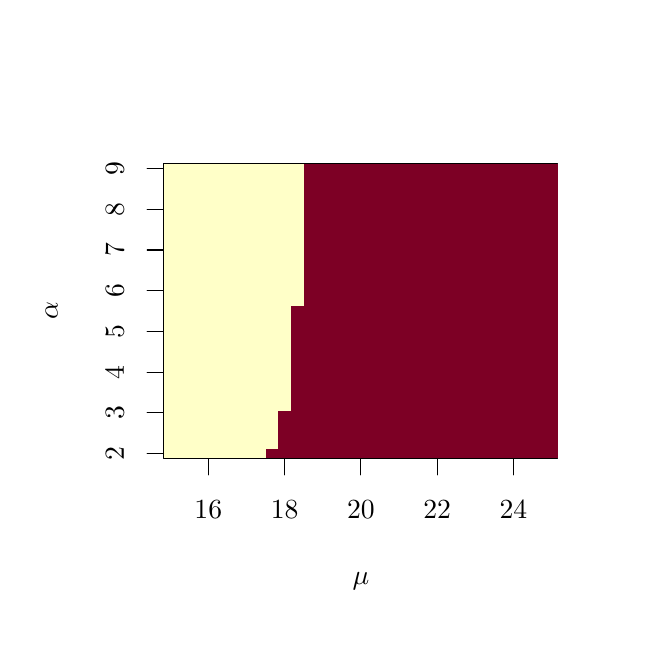
\begin{tikzpicture}[x=1pt,y=1pt]
\definecolor{fillColor}{RGB}{255,255,255}
\path[use as bounding box,fill=fillColor,fill opacity=0.00] (0,0) rectangle (216.81,216.81);
\begin{scope}
\path[clip] (  0.00,  0.00) rectangle (216.81,216.81);
\definecolor{drawColor}{RGB}{0,0,0}

\path[draw=drawColor,line width= 0.4pt,line join=round,line cap=round] ( 65.28, 61.20) -- (175.53, 61.20);

\path[draw=drawColor,line width= 0.4pt,line join=round,line cap=round] ( 65.28, 61.20) -- ( 65.28, 55.20);

\path[draw=drawColor,line width= 0.4pt,line join=round,line cap=round] ( 92.84, 61.20) -- ( 92.84, 55.20);

\path[draw=drawColor,line width= 0.4pt,line join=round,line cap=round] (120.40, 61.20) -- (120.40, 55.20);

\path[draw=drawColor,line width= 0.4pt,line join=round,line cap=round] (147.97, 61.20) -- (147.97, 55.20);

\path[draw=drawColor,line width= 0.4pt,line join=round,line cap=round] (175.53, 61.20) -- (175.53, 55.20);

\node[text=drawColor,anchor=base,inner sep=0pt, outer sep=0pt, scale=  1.00] at ( 65.28, 39.60) {16};

\node[text=drawColor,anchor=base,inner sep=0pt, outer sep=0pt, scale=  1.00] at ( 92.84, 39.60) {18};

\node[text=drawColor,anchor=base,inner sep=0pt, outer sep=0pt, scale=  1.00] at (120.40, 39.60) {20};

\node[text=drawColor,anchor=base,inner sep=0pt, outer sep=0pt, scale=  1.00] at (147.97, 39.60) {22};

\node[text=drawColor,anchor=base,inner sep=0pt, outer sep=0pt, scale=  1.00] at (175.53, 39.60) {24};

\path[draw=drawColor,line width= 0.4pt,line join=round,line cap=round] ( 49.20, 62.92) -- ( 49.20,165.89);

\path[draw=drawColor,line width= 0.4pt,line join=round,line cap=round] ( 49.20, 62.92) -- ( 43.20, 62.92);

\path[draw=drawColor,line width= 0.4pt,line join=round,line cap=round] ( 49.20, 77.63) -- ( 43.20, 77.63);

\path[draw=drawColor,line width= 0.4pt,line join=round,line cap=round] ( 49.20, 92.34) -- ( 43.20, 92.34);

\path[draw=drawColor,line width= 0.4pt,line join=round,line cap=round] ( 49.20,107.05) -- ( 43.20,107.05);

\path[draw=drawColor,line width= 0.4pt,line join=round,line cap=round] ( 49.20,121.76) -- ( 43.20,121.76);

\path[draw=drawColor,line width= 0.4pt,line join=round,line cap=round] ( 49.20,136.47) -- ( 43.20,136.47);

\path[draw=drawColor,line width= 0.4pt,line join=round,line cap=round] ( 49.20,151.18) -- ( 43.20,151.18);

\path[draw=drawColor,line width= 0.4pt,line join=round,line cap=round] ( 49.20,165.89) -- ( 43.20,165.89);

\node[text=drawColor,rotate= 90.00,anchor=base,inner sep=0pt, outer sep=0pt, scale=  1.00] at ( 34.80, 62.92) {2};

\node[text=drawColor,rotate= 90.00,anchor=base,inner sep=0pt, outer sep=0pt, scale=  1.00] at ( 34.80, 77.63) {3};

\node[text=drawColor,rotate= 90.00,anchor=base,inner sep=0pt, outer sep=0pt, scale=  1.00] at ( 34.80, 92.34) {4};

\node[text=drawColor,rotate= 90.00,anchor=base,inner sep=0pt, outer sep=0pt, scale=  1.00] at ( 34.80,107.05) {5};

\node[text=drawColor,rotate= 90.00,anchor=base,inner sep=0pt, outer sep=0pt, scale=  1.00] at ( 34.80,121.76) {6};

\node[text=drawColor,rotate= 90.00,anchor=base,inner sep=0pt, outer sep=0pt, scale=  1.00] at ( 34.80,136.47) {7};

\node[text=drawColor,rotate= 90.00,anchor=base,inner sep=0pt, outer sep=0pt, scale=  1.00] at ( 34.80,151.18) {8};

\node[text=drawColor,rotate= 90.00,anchor=base,inner sep=0pt, outer sep=0pt, scale=  1.00] at ( 34.80,165.89) {9};

\path[draw=drawColor,line width= 0.4pt,line join=round,line cap=round] ( 49.20, 61.20) --
	(191.61, 61.20) --
	(191.61,167.61) --
	( 49.20,167.61) --
	( 49.20, 61.20);
\end{scope}
\begin{scope}
\path[clip] (  0.00,  0.00) rectangle (216.81,216.81);
\definecolor{drawColor}{RGB}{0,0,0}

\node[text=drawColor,anchor=base,inner sep=0pt, outer sep=0pt, scale=  1.00] at (120.40, 15.60) {$\mu$};

\node[text=drawColor,rotate= 90.00,anchor=base,inner sep=0pt, outer sep=0pt, scale=  1.00] at ( 10.80,114.41) {$\alpha$};
\end{scope}
\begin{scope}
\path[clip] ( 49.20, 61.20) rectangle (191.61,167.61);
\definecolor{fillColor}{RGB}{255,255,200}

\path[fill=fillColor] ( 49.20, 61.20) rectangle ( 53.79, 64.63);

\path[fill=fillColor] ( 49.20, 64.63) rectangle ( 53.79, 68.07);

\path[fill=fillColor] ( 49.20, 68.07) rectangle ( 53.79, 71.50);

\path[fill=fillColor] ( 49.20, 71.50) rectangle ( 53.79, 74.93);

\path[fill=fillColor] ( 49.20, 74.93) rectangle ( 53.79, 78.36);

\path[fill=fillColor] ( 49.20, 78.36) rectangle ( 53.79, 81.80);

\path[fill=fillColor] ( 49.20, 81.80) rectangle ( 53.79, 85.23);

\path[fill=fillColor] ( 49.20, 85.23) rectangle ( 53.79, 88.66);

\path[fill=fillColor] ( 49.20, 88.66) rectangle ( 53.79, 92.09);

\path[fill=fillColor] ( 49.20, 92.09) rectangle ( 53.79, 95.53);

\path[fill=fillColor] ( 49.20, 95.53) rectangle ( 53.79, 98.96);

\path[fill=fillColor] ( 49.20, 98.96) rectangle ( 53.79,102.39);

\path[fill=fillColor] ( 49.20,102.39) rectangle ( 53.79,105.82);

\path[fill=fillColor] ( 49.20,105.82) rectangle ( 53.79,109.26);

\path[fill=fillColor] ( 49.20,109.26) rectangle ( 53.79,112.69);

\path[fill=fillColor] ( 49.20,112.69) rectangle ( 53.79,116.12);

\path[fill=fillColor] ( 49.20,116.12) rectangle ( 53.79,119.55);

\path[fill=fillColor] ( 49.20,119.55) rectangle ( 53.79,122.99);

\path[fill=fillColor] ( 49.20,122.99) rectangle ( 53.79,126.42);

\path[fill=fillColor] ( 49.20,126.42) rectangle ( 53.79,129.85);

\path[fill=fillColor] ( 49.20,129.85) rectangle ( 53.79,133.28);

\path[fill=fillColor] ( 49.20,133.28) rectangle ( 53.79,136.72);

\path[fill=fillColor] ( 49.20,136.72) rectangle ( 53.79,140.15);

\path[fill=fillColor] ( 49.20,140.15) rectangle ( 53.79,143.58);

\path[fill=fillColor] ( 49.20,143.58) rectangle ( 53.79,147.01);

\path[fill=fillColor] ( 49.20,147.01) rectangle ( 53.79,150.45);

\path[fill=fillColor] ( 49.20,150.45) rectangle ( 53.79,153.88);

\path[fill=fillColor] ( 49.20,153.88) rectangle ( 53.79,157.31);

\path[fill=fillColor] ( 49.20,157.31) rectangle ( 53.79,160.74);

\path[fill=fillColor] ( 49.20,160.74) rectangle ( 53.79,164.18);

\path[fill=fillColor] ( 49.20,164.18) rectangle ( 53.79,167.61);

\path[fill=fillColor] ( 53.79, 61.20) rectangle ( 58.39, 64.63);

\path[fill=fillColor] ( 53.79, 64.63) rectangle ( 58.39, 68.07);

\path[fill=fillColor] ( 53.79, 68.07) rectangle ( 58.39, 71.50);

\path[fill=fillColor] ( 53.79, 71.50) rectangle ( 58.39, 74.93);

\path[fill=fillColor] ( 53.79, 74.93) rectangle ( 58.39, 78.36);

\path[fill=fillColor] ( 53.79, 78.36) rectangle ( 58.39, 81.80);

\path[fill=fillColor] ( 53.79, 81.80) rectangle ( 58.39, 85.23);

\path[fill=fillColor] ( 53.79, 85.23) rectangle ( 58.39, 88.66);

\path[fill=fillColor] ( 53.79, 88.66) rectangle ( 58.39, 92.09);

\path[fill=fillColor] ( 53.79, 92.09) rectangle ( 58.39, 95.53);

\path[fill=fillColor] ( 53.79, 95.53) rectangle ( 58.39, 98.96);

\path[fill=fillColor] ( 53.79, 98.96) rectangle ( 58.39,102.39);

\path[fill=fillColor] ( 53.79,102.39) rectangle ( 58.39,105.82);

\path[fill=fillColor] ( 53.79,105.82) rectangle ( 58.39,109.26);

\path[fill=fillColor] ( 53.79,109.26) rectangle ( 58.39,112.69);

\path[fill=fillColor] ( 53.79,112.69) rectangle ( 58.39,116.12);

\path[fill=fillColor] ( 53.79,116.12) rectangle ( 58.39,119.55);

\path[fill=fillColor] ( 53.79,119.55) rectangle ( 58.39,122.99);

\path[fill=fillColor] ( 53.79,122.99) rectangle ( 58.39,126.42);

\path[fill=fillColor] ( 53.79,126.42) rectangle ( 58.39,129.85);

\path[fill=fillColor] ( 53.79,129.85) rectangle ( 58.39,133.28);

\path[fill=fillColor] ( 53.79,133.28) rectangle ( 58.39,136.72);

\path[fill=fillColor] ( 53.79,136.72) rectangle ( 58.39,140.15);

\path[fill=fillColor] ( 53.79,140.15) rectangle ( 58.39,143.58);

\path[fill=fillColor] ( 53.79,143.58) rectangle ( 58.39,147.01);

\path[fill=fillColor] ( 53.79,147.01) rectangle ( 58.39,150.45);

\path[fill=fillColor] ( 53.79,150.45) rectangle ( 58.39,153.88);

\path[fill=fillColor] ( 53.79,153.88) rectangle ( 58.39,157.31);

\path[fill=fillColor] ( 53.79,157.31) rectangle ( 58.39,160.74);

\path[fill=fillColor] ( 53.79,160.74) rectangle ( 58.39,164.18);

\path[fill=fillColor] ( 53.79,164.18) rectangle ( 58.39,167.61);

\path[fill=fillColor] ( 58.39, 61.20) rectangle ( 62.98, 64.63);

\path[fill=fillColor] ( 58.39, 64.63) rectangle ( 62.98, 68.07);

\path[fill=fillColor] ( 58.39, 68.07) rectangle ( 62.98, 71.50);

\path[fill=fillColor] ( 58.39, 71.50) rectangle ( 62.98, 74.93);

\path[fill=fillColor] ( 58.39, 74.93) rectangle ( 62.98, 78.36);

\path[fill=fillColor] ( 58.39, 78.36) rectangle ( 62.98, 81.80);

\path[fill=fillColor] ( 58.39, 81.80) rectangle ( 62.98, 85.23);

\path[fill=fillColor] ( 58.39, 85.23) rectangle ( 62.98, 88.66);

\path[fill=fillColor] ( 58.39, 88.66) rectangle ( 62.98, 92.09);

\path[fill=fillColor] ( 58.39, 92.09) rectangle ( 62.98, 95.53);

\path[fill=fillColor] ( 58.39, 95.53) rectangle ( 62.98, 98.96);

\path[fill=fillColor] ( 58.39, 98.96) rectangle ( 62.98,102.39);

\path[fill=fillColor] ( 58.39,102.39) rectangle ( 62.98,105.82);

\path[fill=fillColor] ( 58.39,105.82) rectangle ( 62.98,109.26);

\path[fill=fillColor] ( 58.39,109.26) rectangle ( 62.98,112.69);

\path[fill=fillColor] ( 58.39,112.69) rectangle ( 62.98,116.12);

\path[fill=fillColor] ( 58.39,116.12) rectangle ( 62.98,119.55);

\path[fill=fillColor] ( 58.39,119.55) rectangle ( 62.98,122.99);

\path[fill=fillColor] ( 58.39,122.99) rectangle ( 62.98,126.42);

\path[fill=fillColor] ( 58.39,126.42) rectangle ( 62.98,129.85);

\path[fill=fillColor] ( 58.39,129.85) rectangle ( 62.98,133.28);

\path[fill=fillColor] ( 58.39,133.28) rectangle ( 62.98,136.72);

\path[fill=fillColor] ( 58.39,136.72) rectangle ( 62.98,140.15);

\path[fill=fillColor] ( 58.39,140.15) rectangle ( 62.98,143.58);

\path[fill=fillColor] ( 58.39,143.58) rectangle ( 62.98,147.01);

\path[fill=fillColor] ( 58.39,147.01) rectangle ( 62.98,150.45);

\path[fill=fillColor] ( 58.39,150.45) rectangle ( 62.98,153.88);

\path[fill=fillColor] ( 58.39,153.88) rectangle ( 62.98,157.31);

\path[fill=fillColor] ( 58.39,157.31) rectangle ( 62.98,160.74);

\path[fill=fillColor] ( 58.39,160.74) rectangle ( 62.98,164.18);

\path[fill=fillColor] ( 58.39,164.18) rectangle ( 62.98,167.61);

\path[fill=fillColor] ( 62.98, 61.20) rectangle ( 67.58, 64.63);

\path[fill=fillColor] ( 62.98, 64.63) rectangle ( 67.58, 68.07);

\path[fill=fillColor] ( 62.98, 68.07) rectangle ( 67.58, 71.50);

\path[fill=fillColor] ( 62.98, 71.50) rectangle ( 67.58, 74.93);

\path[fill=fillColor] ( 62.98, 74.93) rectangle ( 67.58, 78.36);

\path[fill=fillColor] ( 62.98, 78.36) rectangle ( 67.58, 81.80);

\path[fill=fillColor] ( 62.98, 81.80) rectangle ( 67.58, 85.23);

\path[fill=fillColor] ( 62.98, 85.23) rectangle ( 67.58, 88.66);

\path[fill=fillColor] ( 62.98, 88.66) rectangle ( 67.58, 92.09);

\path[fill=fillColor] ( 62.98, 92.09) rectangle ( 67.58, 95.53);

\path[fill=fillColor] ( 62.98, 95.53) rectangle ( 67.58, 98.96);

\path[fill=fillColor] ( 62.98, 98.96) rectangle ( 67.58,102.39);

\path[fill=fillColor] ( 62.98,102.39) rectangle ( 67.58,105.82);

\path[fill=fillColor] ( 62.98,105.82) rectangle ( 67.58,109.26);

\path[fill=fillColor] ( 62.98,109.26) rectangle ( 67.58,112.69);

\path[fill=fillColor] ( 62.98,112.69) rectangle ( 67.58,116.12);

\path[fill=fillColor] ( 62.98,116.12) rectangle ( 67.58,119.55);

\path[fill=fillColor] ( 62.98,119.55) rectangle ( 67.58,122.99);

\path[fill=fillColor] ( 62.98,122.99) rectangle ( 67.58,126.42);

\path[fill=fillColor] ( 62.98,126.42) rectangle ( 67.58,129.85);

\path[fill=fillColor] ( 62.98,129.85) rectangle ( 67.58,133.28);

\path[fill=fillColor] ( 62.98,133.28) rectangle ( 67.58,136.72);

\path[fill=fillColor] ( 62.98,136.72) rectangle ( 67.58,140.15);

\path[fill=fillColor] ( 62.98,140.15) rectangle ( 67.58,143.58);

\path[fill=fillColor] ( 62.98,143.58) rectangle ( 67.58,147.01);

\path[fill=fillColor] ( 62.98,147.01) rectangle ( 67.58,150.45);

\path[fill=fillColor] ( 62.98,150.45) rectangle ( 67.58,153.88);

\path[fill=fillColor] ( 62.98,153.88) rectangle ( 67.58,157.31);

\path[fill=fillColor] ( 62.98,157.31) rectangle ( 67.58,160.74);

\path[fill=fillColor] ( 62.98,160.74) rectangle ( 67.58,164.18);

\path[fill=fillColor] ( 62.98,164.18) rectangle ( 67.58,167.61);

\path[fill=fillColor] ( 67.58, 61.20) rectangle ( 72.17, 64.63);

\path[fill=fillColor] ( 67.58, 64.63) rectangle ( 72.17, 68.07);

\path[fill=fillColor] ( 67.58, 68.07) rectangle ( 72.17, 71.50);

\path[fill=fillColor] ( 67.58, 71.50) rectangle ( 72.17, 74.93);

\path[fill=fillColor] ( 67.58, 74.93) rectangle ( 72.17, 78.36);

\path[fill=fillColor] ( 67.58, 78.36) rectangle ( 72.17, 81.80);

\path[fill=fillColor] ( 67.58, 81.80) rectangle ( 72.17, 85.23);

\path[fill=fillColor] ( 67.58, 85.23) rectangle ( 72.17, 88.66);

\path[fill=fillColor] ( 67.58, 88.66) rectangle ( 72.17, 92.09);

\path[fill=fillColor] ( 67.58, 92.09) rectangle ( 72.17, 95.53);

\path[fill=fillColor] ( 67.58, 95.53) rectangle ( 72.17, 98.96);

\path[fill=fillColor] ( 67.58, 98.96) rectangle ( 72.17,102.39);

\path[fill=fillColor] ( 67.58,102.39) rectangle ( 72.17,105.82);

\path[fill=fillColor] ( 67.58,105.82) rectangle ( 72.17,109.26);

\path[fill=fillColor] ( 67.58,109.26) rectangle ( 72.17,112.69);

\path[fill=fillColor] ( 67.58,112.69) rectangle ( 72.17,116.12);

\path[fill=fillColor] ( 67.58,116.12) rectangle ( 72.17,119.55);

\path[fill=fillColor] ( 67.58,119.55) rectangle ( 72.17,122.99);

\path[fill=fillColor] ( 67.58,122.99) rectangle ( 72.17,126.42);

\path[fill=fillColor] ( 67.58,126.42) rectangle ( 72.17,129.85);

\path[fill=fillColor] ( 67.58,129.85) rectangle ( 72.17,133.28);

\path[fill=fillColor] ( 67.58,133.28) rectangle ( 72.17,136.72);

\path[fill=fillColor] ( 67.58,136.72) rectangle ( 72.17,140.15);

\path[fill=fillColor] ( 67.58,140.15) rectangle ( 72.17,143.58);

\path[fill=fillColor] ( 67.58,143.58) rectangle ( 72.17,147.01);

\path[fill=fillColor] ( 67.58,147.01) rectangle ( 72.17,150.45);

\path[fill=fillColor] ( 67.58,150.45) rectangle ( 72.17,153.88);

\path[fill=fillColor] ( 67.58,153.88) rectangle ( 72.17,157.31);

\path[fill=fillColor] ( 67.58,157.31) rectangle ( 72.17,160.74);

\path[fill=fillColor] ( 67.58,160.74) rectangle ( 72.17,164.18);

\path[fill=fillColor] ( 67.58,164.18) rectangle ( 72.17,167.61);

\path[fill=fillColor] ( 72.17, 61.20) rectangle ( 76.76, 64.63);

\path[fill=fillColor] ( 72.17, 64.63) rectangle ( 76.76, 68.07);

\path[fill=fillColor] ( 72.17, 68.07) rectangle ( 76.76, 71.50);

\path[fill=fillColor] ( 72.17, 71.50) rectangle ( 76.76, 74.93);

\path[fill=fillColor] ( 72.17, 74.93) rectangle ( 76.76, 78.36);

\path[fill=fillColor] ( 72.17, 78.36) rectangle ( 76.76, 81.80);

\path[fill=fillColor] ( 72.17, 81.80) rectangle ( 76.76, 85.23);

\path[fill=fillColor] ( 72.17, 85.23) rectangle ( 76.76, 88.66);

\path[fill=fillColor] ( 72.17, 88.66) rectangle ( 76.76, 92.09);

\path[fill=fillColor] ( 72.17, 92.09) rectangle ( 76.76, 95.53);

\path[fill=fillColor] ( 72.17, 95.53) rectangle ( 76.76, 98.96);

\path[fill=fillColor] ( 72.17, 98.96) rectangle ( 76.76,102.39);

\path[fill=fillColor] ( 72.17,102.39) rectangle ( 76.76,105.82);

\path[fill=fillColor] ( 72.17,105.82) rectangle ( 76.76,109.26);

\path[fill=fillColor] ( 72.17,109.26) rectangle ( 76.76,112.69);

\path[fill=fillColor] ( 72.17,112.69) rectangle ( 76.76,116.12);

\path[fill=fillColor] ( 72.17,116.12) rectangle ( 76.76,119.55);

\path[fill=fillColor] ( 72.17,119.55) rectangle ( 76.76,122.99);

\path[fill=fillColor] ( 72.17,122.99) rectangle ( 76.76,126.42);

\path[fill=fillColor] ( 72.17,126.42) rectangle ( 76.76,129.85);

\path[fill=fillColor] ( 72.17,129.85) rectangle ( 76.76,133.28);

\path[fill=fillColor] ( 72.17,133.28) rectangle ( 76.76,136.72);

\path[fill=fillColor] ( 72.17,136.72) rectangle ( 76.76,140.15);

\path[fill=fillColor] ( 72.17,140.15) rectangle ( 76.76,143.58);

\path[fill=fillColor] ( 72.17,143.58) rectangle ( 76.76,147.01);

\path[fill=fillColor] ( 72.17,147.01) rectangle ( 76.76,150.45);

\path[fill=fillColor] ( 72.17,150.45) rectangle ( 76.76,153.88);

\path[fill=fillColor] ( 72.17,153.88) rectangle ( 76.76,157.31);

\path[fill=fillColor] ( 72.17,157.31) rectangle ( 76.76,160.74);

\path[fill=fillColor] ( 72.17,160.74) rectangle ( 76.76,164.18);

\path[fill=fillColor] ( 72.17,164.18) rectangle ( 76.76,167.61);

\path[fill=fillColor] ( 76.76, 61.20) rectangle ( 81.36, 64.63);

\path[fill=fillColor] ( 76.76, 64.63) rectangle ( 81.36, 68.07);

\path[fill=fillColor] ( 76.76, 68.07) rectangle ( 81.36, 71.50);

\path[fill=fillColor] ( 76.76, 71.50) rectangle ( 81.36, 74.93);

\path[fill=fillColor] ( 76.76, 74.93) rectangle ( 81.36, 78.36);

\path[fill=fillColor] ( 76.76, 78.36) rectangle ( 81.36, 81.80);

\path[fill=fillColor] ( 76.76, 81.80) rectangle ( 81.36, 85.23);

\path[fill=fillColor] ( 76.76, 85.23) rectangle ( 81.36, 88.66);

\path[fill=fillColor] ( 76.76, 88.66) rectangle ( 81.36, 92.09);

\path[fill=fillColor] ( 76.76, 92.09) rectangle ( 81.36, 95.53);

\path[fill=fillColor] ( 76.76, 95.53) rectangle ( 81.36, 98.96);

\path[fill=fillColor] ( 76.76, 98.96) rectangle ( 81.36,102.39);

\path[fill=fillColor] ( 76.76,102.39) rectangle ( 81.36,105.82);

\path[fill=fillColor] ( 76.76,105.82) rectangle ( 81.36,109.26);

\path[fill=fillColor] ( 76.76,109.26) rectangle ( 81.36,112.69);

\path[fill=fillColor] ( 76.76,112.69) rectangle ( 81.36,116.12);

\path[fill=fillColor] ( 76.76,116.12) rectangle ( 81.36,119.55);

\path[fill=fillColor] ( 76.76,119.55) rectangle ( 81.36,122.99);

\path[fill=fillColor] ( 76.76,122.99) rectangle ( 81.36,126.42);

\path[fill=fillColor] ( 76.76,126.42) rectangle ( 81.36,129.85);

\path[fill=fillColor] ( 76.76,129.85) rectangle ( 81.36,133.28);

\path[fill=fillColor] ( 76.76,133.28) rectangle ( 81.36,136.72);

\path[fill=fillColor] ( 76.76,136.72) rectangle ( 81.36,140.15);

\path[fill=fillColor] ( 76.76,140.15) rectangle ( 81.36,143.58);

\path[fill=fillColor] ( 76.76,143.58) rectangle ( 81.36,147.01);

\path[fill=fillColor] ( 76.76,147.01) rectangle ( 81.36,150.45);

\path[fill=fillColor] ( 76.76,150.45) rectangle ( 81.36,153.88);

\path[fill=fillColor] ( 76.76,153.88) rectangle ( 81.36,157.31);

\path[fill=fillColor] ( 76.76,157.31) rectangle ( 81.36,160.74);

\path[fill=fillColor] ( 76.76,160.74) rectangle ( 81.36,164.18);

\path[fill=fillColor] ( 76.76,164.18) rectangle ( 81.36,167.61);

\path[fill=fillColor] ( 81.36, 61.20) rectangle ( 85.95, 64.63);

\path[fill=fillColor] ( 81.36, 64.63) rectangle ( 85.95, 68.07);

\path[fill=fillColor] ( 81.36, 68.07) rectangle ( 85.95, 71.50);

\path[fill=fillColor] ( 81.36, 71.50) rectangle ( 85.95, 74.93);

\path[fill=fillColor] ( 81.36, 74.93) rectangle ( 85.95, 78.36);

\path[fill=fillColor] ( 81.36, 78.36) rectangle ( 85.95, 81.80);

\path[fill=fillColor] ( 81.36, 81.80) rectangle ( 85.95, 85.23);

\path[fill=fillColor] ( 81.36, 85.23) rectangle ( 85.95, 88.66);

\path[fill=fillColor] ( 81.36, 88.66) rectangle ( 85.95, 92.09);

\path[fill=fillColor] ( 81.36, 92.09) rectangle ( 85.95, 95.53);

\path[fill=fillColor] ( 81.36, 95.53) rectangle ( 85.95, 98.96);

\path[fill=fillColor] ( 81.36, 98.96) rectangle ( 85.95,102.39);

\path[fill=fillColor] ( 81.36,102.39) rectangle ( 85.95,105.82);

\path[fill=fillColor] ( 81.36,105.82) rectangle ( 85.95,109.26);

\path[fill=fillColor] ( 81.36,109.26) rectangle ( 85.95,112.69);

\path[fill=fillColor] ( 81.36,112.69) rectangle ( 85.95,116.12);

\path[fill=fillColor] ( 81.36,116.12) rectangle ( 85.95,119.55);

\path[fill=fillColor] ( 81.36,119.55) rectangle ( 85.95,122.99);

\path[fill=fillColor] ( 81.36,122.99) rectangle ( 85.95,126.42);

\path[fill=fillColor] ( 81.36,126.42) rectangle ( 85.95,129.85);

\path[fill=fillColor] ( 81.36,129.85) rectangle ( 85.95,133.28);

\path[fill=fillColor] ( 81.36,133.28) rectangle ( 85.95,136.72);

\path[fill=fillColor] ( 81.36,136.72) rectangle ( 85.95,140.15);

\path[fill=fillColor] ( 81.36,140.15) rectangle ( 85.95,143.58);

\path[fill=fillColor] ( 81.36,143.58) rectangle ( 85.95,147.01);

\path[fill=fillColor] ( 81.36,147.01) rectangle ( 85.95,150.45);

\path[fill=fillColor] ( 81.36,150.45) rectangle ( 85.95,153.88);

\path[fill=fillColor] ( 81.36,153.88) rectangle ( 85.95,157.31);

\path[fill=fillColor] ( 81.36,157.31) rectangle ( 85.95,160.74);

\path[fill=fillColor] ( 81.36,160.74) rectangle ( 85.95,164.18);

\path[fill=fillColor] ( 81.36,164.18) rectangle ( 85.95,167.61);
\definecolor{fillColor}{RGB}{125,0,37}

\path[fill=fillColor] ( 85.95, 61.20) rectangle ( 90.54, 64.63);
\definecolor{fillColor}{RGB}{255,255,200}

\path[fill=fillColor] ( 85.95, 64.63) rectangle ( 90.54, 68.07);

\path[fill=fillColor] ( 85.95, 68.07) rectangle ( 90.54, 71.50);

\path[fill=fillColor] ( 85.95, 71.50) rectangle ( 90.54, 74.93);

\path[fill=fillColor] ( 85.95, 74.93) rectangle ( 90.54, 78.36);

\path[fill=fillColor] ( 85.95, 78.36) rectangle ( 90.54, 81.80);

\path[fill=fillColor] ( 85.95, 81.80) rectangle ( 90.54, 85.23);

\path[fill=fillColor] ( 85.95, 85.23) rectangle ( 90.54, 88.66);

\path[fill=fillColor] ( 85.95, 88.66) rectangle ( 90.54, 92.09);

\path[fill=fillColor] ( 85.95, 92.09) rectangle ( 90.54, 95.53);

\path[fill=fillColor] ( 85.95, 95.53) rectangle ( 90.54, 98.96);

\path[fill=fillColor] ( 85.95, 98.96) rectangle ( 90.54,102.39);

\path[fill=fillColor] ( 85.95,102.39) rectangle ( 90.54,105.82);

\path[fill=fillColor] ( 85.95,105.82) rectangle ( 90.54,109.26);

\path[fill=fillColor] ( 85.95,109.26) rectangle ( 90.54,112.69);

\path[fill=fillColor] ( 85.95,112.69) rectangle ( 90.54,116.12);

\path[fill=fillColor] ( 85.95,116.12) rectangle ( 90.54,119.55);

\path[fill=fillColor] ( 85.95,119.55) rectangle ( 90.54,122.99);

\path[fill=fillColor] ( 85.95,122.99) rectangle ( 90.54,126.42);

\path[fill=fillColor] ( 85.95,126.42) rectangle ( 90.54,129.85);

\path[fill=fillColor] ( 85.95,129.85) rectangle ( 90.54,133.28);

\path[fill=fillColor] ( 85.95,133.28) rectangle ( 90.54,136.72);

\path[fill=fillColor] ( 85.95,136.72) rectangle ( 90.54,140.15);

\path[fill=fillColor] ( 85.95,140.15) rectangle ( 90.54,143.58);

\path[fill=fillColor] ( 85.95,143.58) rectangle ( 90.54,147.01);

\path[fill=fillColor] ( 85.95,147.01) rectangle ( 90.54,150.45);

\path[fill=fillColor] ( 85.95,150.45) rectangle ( 90.54,153.88);

\path[fill=fillColor] ( 85.95,153.88) rectangle ( 90.54,157.31);

\path[fill=fillColor] ( 85.95,157.31) rectangle ( 90.54,160.74);

\path[fill=fillColor] ( 85.95,160.74) rectangle ( 90.54,164.18);

\path[fill=fillColor] ( 85.95,164.18) rectangle ( 90.54,167.61);
\definecolor{fillColor}{RGB}{125,0,37}

\path[fill=fillColor] ( 90.54, 61.20) rectangle ( 95.14, 64.63);

\path[fill=fillColor] ( 90.54, 64.63) rectangle ( 95.14, 68.07);

\path[fill=fillColor] ( 90.54, 68.07) rectangle ( 95.14, 71.50);

\path[fill=fillColor] ( 90.54, 71.50) rectangle ( 95.14, 74.93);

\path[fill=fillColor] ( 90.54, 74.93) rectangle ( 95.14, 78.36);
\definecolor{fillColor}{RGB}{255,255,200}

\path[fill=fillColor] ( 90.54, 78.36) rectangle ( 95.14, 81.80);

\path[fill=fillColor] ( 90.54, 81.80) rectangle ( 95.14, 85.23);

\path[fill=fillColor] ( 90.54, 85.23) rectangle ( 95.14, 88.66);

\path[fill=fillColor] ( 90.54, 88.66) rectangle ( 95.14, 92.09);

\path[fill=fillColor] ( 90.54, 92.09) rectangle ( 95.14, 95.53);

\path[fill=fillColor] ( 90.54, 95.53) rectangle ( 95.14, 98.96);

\path[fill=fillColor] ( 90.54, 98.96) rectangle ( 95.14,102.39);

\path[fill=fillColor] ( 90.54,102.39) rectangle ( 95.14,105.82);

\path[fill=fillColor] ( 90.54,105.82) rectangle ( 95.14,109.26);

\path[fill=fillColor] ( 90.54,109.26) rectangle ( 95.14,112.69);

\path[fill=fillColor] ( 90.54,112.69) rectangle ( 95.14,116.12);

\path[fill=fillColor] ( 90.54,116.12) rectangle ( 95.14,119.55);

\path[fill=fillColor] ( 90.54,119.55) rectangle ( 95.14,122.99);

\path[fill=fillColor] ( 90.54,122.99) rectangle ( 95.14,126.42);

\path[fill=fillColor] ( 90.54,126.42) rectangle ( 95.14,129.85);

\path[fill=fillColor] ( 90.54,129.85) rectangle ( 95.14,133.28);

\path[fill=fillColor] ( 90.54,133.28) rectangle ( 95.14,136.72);

\path[fill=fillColor] ( 90.54,136.72) rectangle ( 95.14,140.15);

\path[fill=fillColor] ( 90.54,140.15) rectangle ( 95.14,143.58);

\path[fill=fillColor] ( 90.54,143.58) rectangle ( 95.14,147.01);

\path[fill=fillColor] ( 90.54,147.01) rectangle ( 95.14,150.45);

\path[fill=fillColor] ( 90.54,150.45) rectangle ( 95.14,153.88);

\path[fill=fillColor] ( 90.54,153.88) rectangle ( 95.14,157.31);

\path[fill=fillColor] ( 90.54,157.31) rectangle ( 95.14,160.74);

\path[fill=fillColor] ( 90.54,160.74) rectangle ( 95.14,164.18);

\path[fill=fillColor] ( 90.54,164.18) rectangle ( 95.14,167.61);
\definecolor{fillColor}{RGB}{125,0,37}

\path[fill=fillColor] ( 95.14, 61.20) rectangle ( 99.73, 64.63);

\path[fill=fillColor] ( 95.14, 64.63) rectangle ( 99.73, 68.07);

\path[fill=fillColor] ( 95.14, 68.07) rectangle ( 99.73, 71.50);

\path[fill=fillColor] ( 95.14, 71.50) rectangle ( 99.73, 74.93);

\path[fill=fillColor] ( 95.14, 74.93) rectangle ( 99.73, 78.36);

\path[fill=fillColor] ( 95.14, 78.36) rectangle ( 99.73, 81.80);

\path[fill=fillColor] ( 95.14, 81.80) rectangle ( 99.73, 85.23);

\path[fill=fillColor] ( 95.14, 85.23) rectangle ( 99.73, 88.66);

\path[fill=fillColor] ( 95.14, 88.66) rectangle ( 99.73, 92.09);

\path[fill=fillColor] ( 95.14, 92.09) rectangle ( 99.73, 95.53);

\path[fill=fillColor] ( 95.14, 95.53) rectangle ( 99.73, 98.96);

\path[fill=fillColor] ( 95.14, 98.96) rectangle ( 99.73,102.39);

\path[fill=fillColor] ( 95.14,102.39) rectangle ( 99.73,105.82);

\path[fill=fillColor] ( 95.14,105.82) rectangle ( 99.73,109.26);

\path[fill=fillColor] ( 95.14,109.26) rectangle ( 99.73,112.69);

\path[fill=fillColor] ( 95.14,112.69) rectangle ( 99.73,116.12);
\definecolor{fillColor}{RGB}{255,255,200}

\path[fill=fillColor] ( 95.14,116.12) rectangle ( 99.73,119.55);

\path[fill=fillColor] ( 95.14,119.55) rectangle ( 99.73,122.99);

\path[fill=fillColor] ( 95.14,122.99) rectangle ( 99.73,126.42);

\path[fill=fillColor] ( 95.14,126.42) rectangle ( 99.73,129.85);

\path[fill=fillColor] ( 95.14,129.85) rectangle ( 99.73,133.28);

\path[fill=fillColor] ( 95.14,133.28) rectangle ( 99.73,136.72);

\path[fill=fillColor] ( 95.14,136.72) rectangle ( 99.73,140.15);

\path[fill=fillColor] ( 95.14,140.15) rectangle ( 99.73,143.58);

\path[fill=fillColor] ( 95.14,143.58) rectangle ( 99.73,147.01);

\path[fill=fillColor] ( 95.14,147.01) rectangle ( 99.73,150.45);

\path[fill=fillColor] ( 95.14,150.45) rectangle ( 99.73,153.88);

\path[fill=fillColor] ( 95.14,153.88) rectangle ( 99.73,157.31);

\path[fill=fillColor] ( 95.14,157.31) rectangle ( 99.73,160.74);

\path[fill=fillColor] ( 95.14,160.74) rectangle ( 99.73,164.18);

\path[fill=fillColor] ( 95.14,164.18) rectangle ( 99.73,167.61);
\definecolor{fillColor}{RGB}{125,0,37}

\path[fill=fillColor] ( 99.73, 61.20) rectangle (104.33, 64.63);

\path[fill=fillColor] ( 99.73, 64.63) rectangle (104.33, 68.07);

\path[fill=fillColor] ( 99.73, 68.07) rectangle (104.33, 71.50);

\path[fill=fillColor] ( 99.73, 71.50) rectangle (104.33, 74.93);

\path[fill=fillColor] ( 99.73, 74.93) rectangle (104.33, 78.36);

\path[fill=fillColor] ( 99.73, 78.36) rectangle (104.33, 81.80);

\path[fill=fillColor] ( 99.73, 81.80) rectangle (104.33, 85.23);

\path[fill=fillColor] ( 99.73, 85.23) rectangle (104.33, 88.66);

\path[fill=fillColor] ( 99.73, 88.66) rectangle (104.33, 92.09);

\path[fill=fillColor] ( 99.73, 92.09) rectangle (104.33, 95.53);

\path[fill=fillColor] ( 99.73, 95.53) rectangle (104.33, 98.96);

\path[fill=fillColor] ( 99.73, 98.96) rectangle (104.33,102.39);

\path[fill=fillColor] ( 99.73,102.39) rectangle (104.33,105.82);

\path[fill=fillColor] ( 99.73,105.82) rectangle (104.33,109.26);

\path[fill=fillColor] ( 99.73,109.26) rectangle (104.33,112.69);

\path[fill=fillColor] ( 99.73,112.69) rectangle (104.33,116.12);

\path[fill=fillColor] ( 99.73,116.12) rectangle (104.33,119.55);

\path[fill=fillColor] ( 99.73,119.55) rectangle (104.33,122.99);

\path[fill=fillColor] ( 99.73,122.99) rectangle (104.33,126.42);

\path[fill=fillColor] ( 99.73,126.42) rectangle (104.33,129.85);

\path[fill=fillColor] ( 99.73,129.85) rectangle (104.33,133.28);

\path[fill=fillColor] ( 99.73,133.28) rectangle (104.33,136.72);

\path[fill=fillColor] ( 99.73,136.72) rectangle (104.33,140.15);

\path[fill=fillColor] ( 99.73,140.15) rectangle (104.33,143.58);

\path[fill=fillColor] ( 99.73,143.58) rectangle (104.33,147.01);

\path[fill=fillColor] ( 99.73,147.01) rectangle (104.33,150.45);

\path[fill=fillColor] ( 99.73,150.45) rectangle (104.33,153.88);

\path[fill=fillColor] ( 99.73,153.88) rectangle (104.33,157.31);

\path[fill=fillColor] ( 99.73,157.31) rectangle (104.33,160.74);

\path[fill=fillColor] ( 99.73,160.74) rectangle (104.33,164.18);

\path[fill=fillColor] ( 99.73,164.18) rectangle (104.33,167.61);

\path[fill=fillColor] (104.33, 61.20) rectangle (108.92, 64.63);

\path[fill=fillColor] (104.33, 64.63) rectangle (108.92, 68.07);

\path[fill=fillColor] (104.33, 68.07) rectangle (108.92, 71.50);

\path[fill=fillColor] (104.33, 71.50) rectangle (108.92, 74.93);

\path[fill=fillColor] (104.33, 74.93) rectangle (108.92, 78.36);

\path[fill=fillColor] (104.33, 78.36) rectangle (108.92, 81.80);

\path[fill=fillColor] (104.33, 81.80) rectangle (108.92, 85.23);

\path[fill=fillColor] (104.33, 85.23) rectangle (108.92, 88.66);

\path[fill=fillColor] (104.33, 88.66) rectangle (108.92, 92.09);

\path[fill=fillColor] (104.33, 92.09) rectangle (108.92, 95.53);

\path[fill=fillColor] (104.33, 95.53) rectangle (108.92, 98.96);

\path[fill=fillColor] (104.33, 98.96) rectangle (108.92,102.39);

\path[fill=fillColor] (104.33,102.39) rectangle (108.92,105.82);

\path[fill=fillColor] (104.33,105.82) rectangle (108.92,109.26);

\path[fill=fillColor] (104.33,109.26) rectangle (108.92,112.69);

\path[fill=fillColor] (104.33,112.69) rectangle (108.92,116.12);

\path[fill=fillColor] (104.33,116.12) rectangle (108.92,119.55);

\path[fill=fillColor] (104.33,119.55) rectangle (108.92,122.99);

\path[fill=fillColor] (104.33,122.99) rectangle (108.92,126.42);

\path[fill=fillColor] (104.33,126.42) rectangle (108.92,129.85);

\path[fill=fillColor] (104.33,129.85) rectangle (108.92,133.28);

\path[fill=fillColor] (104.33,133.28) rectangle (108.92,136.72);

\path[fill=fillColor] (104.33,136.72) rectangle (108.92,140.15);

\path[fill=fillColor] (104.33,140.15) rectangle (108.92,143.58);

\path[fill=fillColor] (104.33,143.58) rectangle (108.92,147.01);

\path[fill=fillColor] (104.33,147.01) rectangle (108.92,150.45);

\path[fill=fillColor] (104.33,150.45) rectangle (108.92,153.88);

\path[fill=fillColor] (104.33,153.88) rectangle (108.92,157.31);

\path[fill=fillColor] (104.33,157.31) rectangle (108.92,160.74);

\path[fill=fillColor] (104.33,160.74) rectangle (108.92,164.18);

\path[fill=fillColor] (104.33,164.18) rectangle (108.92,167.61);

\path[fill=fillColor] (108.92, 61.20) rectangle (113.51, 64.63);

\path[fill=fillColor] (108.92, 64.63) rectangle (113.51, 68.07);

\path[fill=fillColor] (108.92, 68.07) rectangle (113.51, 71.50);

\path[fill=fillColor] (108.92, 71.50) rectangle (113.51, 74.93);

\path[fill=fillColor] (108.92, 74.93) rectangle (113.51, 78.36);

\path[fill=fillColor] (108.92, 78.36) rectangle (113.51, 81.80);

\path[fill=fillColor] (108.92, 81.80) rectangle (113.51, 85.23);

\path[fill=fillColor] (108.92, 85.23) rectangle (113.51, 88.66);

\path[fill=fillColor] (108.92, 88.66) rectangle (113.51, 92.09);

\path[fill=fillColor] (108.92, 92.09) rectangle (113.51, 95.53);

\path[fill=fillColor] (108.92, 95.53) rectangle (113.51, 98.96);

\path[fill=fillColor] (108.92, 98.96) rectangle (113.51,102.39);

\path[fill=fillColor] (108.92,102.39) rectangle (113.51,105.82);

\path[fill=fillColor] (108.92,105.82) rectangle (113.51,109.26);

\path[fill=fillColor] (108.92,109.26) rectangle (113.51,112.69);

\path[fill=fillColor] (108.92,112.69) rectangle (113.51,116.12);

\path[fill=fillColor] (108.92,116.12) rectangle (113.51,119.55);

\path[fill=fillColor] (108.92,119.55) rectangle (113.51,122.99);

\path[fill=fillColor] (108.92,122.99) rectangle (113.51,126.42);

\path[fill=fillColor] (108.92,126.42) rectangle (113.51,129.85);

\path[fill=fillColor] (108.92,129.85) rectangle (113.51,133.28);

\path[fill=fillColor] (108.92,133.28) rectangle (113.51,136.72);

\path[fill=fillColor] (108.92,136.72) rectangle (113.51,140.15);

\path[fill=fillColor] (108.92,140.15) rectangle (113.51,143.58);

\path[fill=fillColor] (108.92,143.58) rectangle (113.51,147.01);

\path[fill=fillColor] (108.92,147.01) rectangle (113.51,150.45);

\path[fill=fillColor] (108.92,150.45) rectangle (113.51,153.88);

\path[fill=fillColor] (108.92,153.88) rectangle (113.51,157.31);

\path[fill=fillColor] (108.92,157.31) rectangle (113.51,160.74);

\path[fill=fillColor] (108.92,160.74) rectangle (113.51,164.18);

\path[fill=fillColor] (108.92,164.18) rectangle (113.51,167.61);

\path[fill=fillColor] (113.51, 61.20) rectangle (118.11, 64.63);

\path[fill=fillColor] (113.51, 64.63) rectangle (118.11, 68.07);

\path[fill=fillColor] (113.51, 68.07) rectangle (118.11, 71.50);

\path[fill=fillColor] (113.51, 71.50) rectangle (118.11, 74.93);

\path[fill=fillColor] (113.51, 74.93) rectangle (118.11, 78.36);

\path[fill=fillColor] (113.51, 78.36) rectangle (118.11, 81.80);

\path[fill=fillColor] (113.51, 81.80) rectangle (118.11, 85.23);

\path[fill=fillColor] (113.51, 85.23) rectangle (118.11, 88.66);

\path[fill=fillColor] (113.51, 88.66) rectangle (118.11, 92.09);

\path[fill=fillColor] (113.51, 92.09) rectangle (118.11, 95.53);

\path[fill=fillColor] (113.51, 95.53) rectangle (118.11, 98.96);

\path[fill=fillColor] (113.51, 98.96) rectangle (118.11,102.39);

\path[fill=fillColor] (113.51,102.39) rectangle (118.11,105.82);

\path[fill=fillColor] (113.51,105.82) rectangle (118.11,109.26);

\path[fill=fillColor] (113.51,109.26) rectangle (118.11,112.69);

\path[fill=fillColor] (113.51,112.69) rectangle (118.11,116.12);

\path[fill=fillColor] (113.51,116.12) rectangle (118.11,119.55);

\path[fill=fillColor] (113.51,119.55) rectangle (118.11,122.99);

\path[fill=fillColor] (113.51,122.99) rectangle (118.11,126.42);

\path[fill=fillColor] (113.51,126.42) rectangle (118.11,129.85);

\path[fill=fillColor] (113.51,129.85) rectangle (118.11,133.28);

\path[fill=fillColor] (113.51,133.28) rectangle (118.11,136.72);

\path[fill=fillColor] (113.51,136.72) rectangle (118.11,140.15);

\path[fill=fillColor] (113.51,140.15) rectangle (118.11,143.58);

\path[fill=fillColor] (113.51,143.58) rectangle (118.11,147.01);

\path[fill=fillColor] (113.51,147.01) rectangle (118.11,150.45);

\path[fill=fillColor] (113.51,150.45) rectangle (118.11,153.88);

\path[fill=fillColor] (113.51,153.88) rectangle (118.11,157.31);

\path[fill=fillColor] (113.51,157.31) rectangle (118.11,160.74);

\path[fill=fillColor] (113.51,160.74) rectangle (118.11,164.18);

\path[fill=fillColor] (113.51,164.18) rectangle (118.11,167.61);

\path[fill=fillColor] (118.11, 61.20) rectangle (122.70, 64.63);

\path[fill=fillColor] (118.11, 64.63) rectangle (122.70, 68.07);

\path[fill=fillColor] (118.11, 68.07) rectangle (122.70, 71.50);

\path[fill=fillColor] (118.11, 71.50) rectangle (122.70, 74.93);

\path[fill=fillColor] (118.11, 74.93) rectangle (122.70, 78.36);

\path[fill=fillColor] (118.11, 78.36) rectangle (122.70, 81.80);

\path[fill=fillColor] (118.11, 81.80) rectangle (122.70, 85.23);

\path[fill=fillColor] (118.11, 85.23) rectangle (122.70, 88.66);

\path[fill=fillColor] (118.11, 88.66) rectangle (122.70, 92.09);

\path[fill=fillColor] (118.11, 92.09) rectangle (122.70, 95.53);

\path[fill=fillColor] (118.11, 95.53) rectangle (122.70, 98.96);

\path[fill=fillColor] (118.11, 98.96) rectangle (122.70,102.39);

\path[fill=fillColor] (118.11,102.39) rectangle (122.70,105.82);

\path[fill=fillColor] (118.11,105.82) rectangle (122.70,109.26);

\path[fill=fillColor] (118.11,109.26) rectangle (122.70,112.69);

\path[fill=fillColor] (118.11,112.69) rectangle (122.70,116.12);

\path[fill=fillColor] (118.11,116.12) rectangle (122.70,119.55);

\path[fill=fillColor] (118.11,119.55) rectangle (122.70,122.99);

\path[fill=fillColor] (118.11,122.99) rectangle (122.70,126.42);

\path[fill=fillColor] (118.11,126.42) rectangle (122.70,129.85);

\path[fill=fillColor] (118.11,129.85) rectangle (122.70,133.28);

\path[fill=fillColor] (118.11,133.28) rectangle (122.70,136.72);

\path[fill=fillColor] (118.11,136.72) rectangle (122.70,140.15);

\path[fill=fillColor] (118.11,140.15) rectangle (122.70,143.58);

\path[fill=fillColor] (118.11,143.58) rectangle (122.70,147.01);

\path[fill=fillColor] (118.11,147.01) rectangle (122.70,150.45);

\path[fill=fillColor] (118.11,150.45) rectangle (122.70,153.88);

\path[fill=fillColor] (118.11,153.88) rectangle (122.70,157.31);

\path[fill=fillColor] (118.11,157.31) rectangle (122.70,160.74);

\path[fill=fillColor] (118.11,160.74) rectangle (122.70,164.18);

\path[fill=fillColor] (118.11,164.18) rectangle (122.70,167.61);

\path[fill=fillColor] (122.70, 61.20) rectangle (127.30, 64.63);

\path[fill=fillColor] (122.70, 64.63) rectangle (127.30, 68.07);

\path[fill=fillColor] (122.70, 68.07) rectangle (127.30, 71.50);

\path[fill=fillColor] (122.70, 71.50) rectangle (127.30, 74.93);

\path[fill=fillColor] (122.70, 74.93) rectangle (127.30, 78.36);

\path[fill=fillColor] (122.70, 78.36) rectangle (127.30, 81.80);

\path[fill=fillColor] (122.70, 81.80) rectangle (127.30, 85.23);

\path[fill=fillColor] (122.70, 85.23) rectangle (127.30, 88.66);

\path[fill=fillColor] (122.70, 88.66) rectangle (127.30, 92.09);

\path[fill=fillColor] (122.70, 92.09) rectangle (127.30, 95.53);

\path[fill=fillColor] (122.70, 95.53) rectangle (127.30, 98.96);

\path[fill=fillColor] (122.70, 98.96) rectangle (127.30,102.39);

\path[fill=fillColor] (122.70,102.39) rectangle (127.30,105.82);

\path[fill=fillColor] (122.70,105.82) rectangle (127.30,109.26);

\path[fill=fillColor] (122.70,109.26) rectangle (127.30,112.69);

\path[fill=fillColor] (122.70,112.69) rectangle (127.30,116.12);

\path[fill=fillColor] (122.70,116.12) rectangle (127.30,119.55);

\path[fill=fillColor] (122.70,119.55) rectangle (127.30,122.99);

\path[fill=fillColor] (122.70,122.99) rectangle (127.30,126.42);

\path[fill=fillColor] (122.70,126.42) rectangle (127.30,129.85);

\path[fill=fillColor] (122.70,129.85) rectangle (127.30,133.28);

\path[fill=fillColor] (122.70,133.28) rectangle (127.30,136.72);

\path[fill=fillColor] (122.70,136.72) rectangle (127.30,140.15);

\path[fill=fillColor] (122.70,140.15) rectangle (127.30,143.58);

\path[fill=fillColor] (122.70,143.58) rectangle (127.30,147.01);

\path[fill=fillColor] (122.70,147.01) rectangle (127.30,150.45);

\path[fill=fillColor] (122.70,150.45) rectangle (127.30,153.88);

\path[fill=fillColor] (122.70,153.88) rectangle (127.30,157.31);

\path[fill=fillColor] (122.70,157.31) rectangle (127.30,160.74);

\path[fill=fillColor] (122.70,160.74) rectangle (127.30,164.18);

\path[fill=fillColor] (122.70,164.18) rectangle (127.30,167.61);

\path[fill=fillColor] (127.30, 61.20) rectangle (131.89, 64.63);

\path[fill=fillColor] (127.30, 64.63) rectangle (131.89, 68.07);

\path[fill=fillColor] (127.30, 68.07) rectangle (131.89, 71.50);

\path[fill=fillColor] (127.30, 71.50) rectangle (131.89, 74.93);

\path[fill=fillColor] (127.30, 74.93) rectangle (131.89, 78.36);

\path[fill=fillColor] (127.30, 78.36) rectangle (131.89, 81.80);

\path[fill=fillColor] (127.30, 81.80) rectangle (131.89, 85.23);

\path[fill=fillColor] (127.30, 85.23) rectangle (131.89, 88.66);

\path[fill=fillColor] (127.30, 88.66) rectangle (131.89, 92.09);

\path[fill=fillColor] (127.30, 92.09) rectangle (131.89, 95.53);

\path[fill=fillColor] (127.30, 95.53) rectangle (131.89, 98.96);

\path[fill=fillColor] (127.30, 98.96) rectangle (131.89,102.39);

\path[fill=fillColor] (127.30,102.39) rectangle (131.89,105.82);

\path[fill=fillColor] (127.30,105.82) rectangle (131.89,109.26);

\path[fill=fillColor] (127.30,109.26) rectangle (131.89,112.69);

\path[fill=fillColor] (127.30,112.69) rectangle (131.89,116.12);

\path[fill=fillColor] (127.30,116.12) rectangle (131.89,119.55);

\path[fill=fillColor] (127.30,119.55) rectangle (131.89,122.99);

\path[fill=fillColor] (127.30,122.99) rectangle (131.89,126.42);

\path[fill=fillColor] (127.30,126.42) rectangle (131.89,129.85);

\path[fill=fillColor] (127.30,129.85) rectangle (131.89,133.28);

\path[fill=fillColor] (127.30,133.28) rectangle (131.89,136.72);

\path[fill=fillColor] (127.30,136.72) rectangle (131.89,140.15);

\path[fill=fillColor] (127.30,140.15) rectangle (131.89,143.58);

\path[fill=fillColor] (127.30,143.58) rectangle (131.89,147.01);

\path[fill=fillColor] (127.30,147.01) rectangle (131.89,150.45);

\path[fill=fillColor] (127.30,150.45) rectangle (131.89,153.88);

\path[fill=fillColor] (127.30,153.88) rectangle (131.89,157.31);

\path[fill=fillColor] (127.30,157.31) rectangle (131.89,160.74);

\path[fill=fillColor] (127.30,160.74) rectangle (131.89,164.18);

\path[fill=fillColor] (127.30,164.18) rectangle (131.89,167.61);

\path[fill=fillColor] (131.89, 61.20) rectangle (136.48, 64.63);

\path[fill=fillColor] (131.89, 64.63) rectangle (136.48, 68.07);

\path[fill=fillColor] (131.89, 68.07) rectangle (136.48, 71.50);

\path[fill=fillColor] (131.89, 71.50) rectangle (136.48, 74.93);

\path[fill=fillColor] (131.89, 74.93) rectangle (136.48, 78.36);

\path[fill=fillColor] (131.89, 78.36) rectangle (136.48, 81.80);

\path[fill=fillColor] (131.89, 81.80) rectangle (136.48, 85.23);

\path[fill=fillColor] (131.89, 85.23) rectangle (136.48, 88.66);

\path[fill=fillColor] (131.89, 88.66) rectangle (136.48, 92.09);

\path[fill=fillColor] (131.89, 92.09) rectangle (136.48, 95.53);

\path[fill=fillColor] (131.89, 95.53) rectangle (136.48, 98.96);

\path[fill=fillColor] (131.89, 98.96) rectangle (136.48,102.39);

\path[fill=fillColor] (131.89,102.39) rectangle (136.48,105.82);

\path[fill=fillColor] (131.89,105.82) rectangle (136.48,109.26);

\path[fill=fillColor] (131.89,109.26) rectangle (136.48,112.69);

\path[fill=fillColor] (131.89,112.69) rectangle (136.48,116.12);

\path[fill=fillColor] (131.89,116.12) rectangle (136.48,119.55);

\path[fill=fillColor] (131.89,119.55) rectangle (136.48,122.99);

\path[fill=fillColor] (131.89,122.99) rectangle (136.48,126.42);

\path[fill=fillColor] (131.89,126.42) rectangle (136.48,129.85);

\path[fill=fillColor] (131.89,129.85) rectangle (136.48,133.28);

\path[fill=fillColor] (131.89,133.28) rectangle (136.48,136.72);

\path[fill=fillColor] (131.89,136.72) rectangle (136.48,140.15);

\path[fill=fillColor] (131.89,140.15) rectangle (136.48,143.58);

\path[fill=fillColor] (131.89,143.58) rectangle (136.48,147.01);

\path[fill=fillColor] (131.89,147.01) rectangle (136.48,150.45);

\path[fill=fillColor] (131.89,150.45) rectangle (136.48,153.88);

\path[fill=fillColor] (131.89,153.88) rectangle (136.48,157.31);

\path[fill=fillColor] (131.89,157.31) rectangle (136.48,160.74);

\path[fill=fillColor] (131.89,160.74) rectangle (136.48,164.18);

\path[fill=fillColor] (131.89,164.18) rectangle (136.48,167.61);

\path[fill=fillColor] (136.48, 61.20) rectangle (141.08, 64.63);

\path[fill=fillColor] (136.48, 64.63) rectangle (141.08, 68.07);

\path[fill=fillColor] (136.48, 68.07) rectangle (141.08, 71.50);

\path[fill=fillColor] (136.48, 71.50) rectangle (141.08, 74.93);

\path[fill=fillColor] (136.48, 74.93) rectangle (141.08, 78.36);

\path[fill=fillColor] (136.48, 78.36) rectangle (141.08, 81.80);

\path[fill=fillColor] (136.48, 81.80) rectangle (141.08, 85.23);

\path[fill=fillColor] (136.48, 85.23) rectangle (141.08, 88.66);

\path[fill=fillColor] (136.48, 88.66) rectangle (141.08, 92.09);

\path[fill=fillColor] (136.48, 92.09) rectangle (141.08, 95.53);

\path[fill=fillColor] (136.48, 95.53) rectangle (141.08, 98.96);

\path[fill=fillColor] (136.48, 98.96) rectangle (141.08,102.39);

\path[fill=fillColor] (136.48,102.39) rectangle (141.08,105.82);

\path[fill=fillColor] (136.48,105.82) rectangle (141.08,109.26);

\path[fill=fillColor] (136.48,109.26) rectangle (141.08,112.69);

\path[fill=fillColor] (136.48,112.69) rectangle (141.08,116.12);

\path[fill=fillColor] (136.48,116.12) rectangle (141.08,119.55);

\path[fill=fillColor] (136.48,119.55) rectangle (141.08,122.99);

\path[fill=fillColor] (136.48,122.99) rectangle (141.08,126.42);

\path[fill=fillColor] (136.48,126.42) rectangle (141.08,129.85);

\path[fill=fillColor] (136.48,129.85) rectangle (141.08,133.28);

\path[fill=fillColor] (136.48,133.28) rectangle (141.08,136.72);

\path[fill=fillColor] (136.48,136.72) rectangle (141.08,140.15);

\path[fill=fillColor] (136.48,140.15) rectangle (141.08,143.58);

\path[fill=fillColor] (136.48,143.58) rectangle (141.08,147.01);

\path[fill=fillColor] (136.48,147.01) rectangle (141.08,150.45);

\path[fill=fillColor] (136.48,150.45) rectangle (141.08,153.88);

\path[fill=fillColor] (136.48,153.88) rectangle (141.08,157.31);

\path[fill=fillColor] (136.48,157.31) rectangle (141.08,160.74);

\path[fill=fillColor] (136.48,160.74) rectangle (141.08,164.18);

\path[fill=fillColor] (136.48,164.18) rectangle (141.08,167.61);

\path[fill=fillColor] (141.08, 61.20) rectangle (145.67, 64.63);

\path[fill=fillColor] (141.08, 64.63) rectangle (145.67, 68.07);

\path[fill=fillColor] (141.08, 68.07) rectangle (145.67, 71.50);

\path[fill=fillColor] (141.08, 71.50) rectangle (145.67, 74.93);

\path[fill=fillColor] (141.08, 74.93) rectangle (145.67, 78.36);

\path[fill=fillColor] (141.08, 78.36) rectangle (145.67, 81.80);

\path[fill=fillColor] (141.08, 81.80) rectangle (145.67, 85.23);

\path[fill=fillColor] (141.08, 85.23) rectangle (145.67, 88.66);

\path[fill=fillColor] (141.08, 88.66) rectangle (145.67, 92.09);

\path[fill=fillColor] (141.08, 92.09) rectangle (145.67, 95.53);

\path[fill=fillColor] (141.08, 95.53) rectangle (145.67, 98.96);

\path[fill=fillColor] (141.08, 98.96) rectangle (145.67,102.39);

\path[fill=fillColor] (141.08,102.39) rectangle (145.67,105.82);

\path[fill=fillColor] (141.08,105.82) rectangle (145.67,109.26);

\path[fill=fillColor] (141.08,109.26) rectangle (145.67,112.69);

\path[fill=fillColor] (141.08,112.69) rectangle (145.67,116.12);

\path[fill=fillColor] (141.08,116.12) rectangle (145.67,119.55);

\path[fill=fillColor] (141.08,119.55) rectangle (145.67,122.99);

\path[fill=fillColor] (141.08,122.99) rectangle (145.67,126.42);

\path[fill=fillColor] (141.08,126.42) rectangle (145.67,129.85);

\path[fill=fillColor] (141.08,129.85) rectangle (145.67,133.28);

\path[fill=fillColor] (141.08,133.28) rectangle (145.67,136.72);

\path[fill=fillColor] (141.08,136.72) rectangle (145.67,140.15);

\path[fill=fillColor] (141.08,140.15) rectangle (145.67,143.58);

\path[fill=fillColor] (141.08,143.58) rectangle (145.67,147.01);

\path[fill=fillColor] (141.08,147.01) rectangle (145.67,150.45);

\path[fill=fillColor] (141.08,150.45) rectangle (145.67,153.88);

\path[fill=fillColor] (141.08,153.88) rectangle (145.67,157.31);

\path[fill=fillColor] (141.08,157.31) rectangle (145.67,160.74);

\path[fill=fillColor] (141.08,160.74) rectangle (145.67,164.18);

\path[fill=fillColor] (141.08,164.18) rectangle (145.67,167.61);

\path[fill=fillColor] (145.67, 61.20) rectangle (150.27, 64.63);

\path[fill=fillColor] (145.67, 64.63) rectangle (150.27, 68.07);

\path[fill=fillColor] (145.67, 68.07) rectangle (150.27, 71.50);

\path[fill=fillColor] (145.67, 71.50) rectangle (150.27, 74.93);

\path[fill=fillColor] (145.67, 74.93) rectangle (150.27, 78.36);

\path[fill=fillColor] (145.67, 78.36) rectangle (150.27, 81.80);

\path[fill=fillColor] (145.67, 81.80) rectangle (150.27, 85.23);

\path[fill=fillColor] (145.67, 85.23) rectangle (150.27, 88.66);

\path[fill=fillColor] (145.67, 88.66) rectangle (150.27, 92.09);

\path[fill=fillColor] (145.67, 92.09) rectangle (150.27, 95.53);

\path[fill=fillColor] (145.67, 95.53) rectangle (150.27, 98.96);

\path[fill=fillColor] (145.67, 98.96) rectangle (150.27,102.39);

\path[fill=fillColor] (145.67,102.39) rectangle (150.27,105.82);

\path[fill=fillColor] (145.67,105.82) rectangle (150.27,109.26);

\path[fill=fillColor] (145.67,109.26) rectangle (150.27,112.69);

\path[fill=fillColor] (145.67,112.69) rectangle (150.27,116.12);

\path[fill=fillColor] (145.67,116.12) rectangle (150.27,119.55);

\path[fill=fillColor] (145.67,119.55) rectangle (150.27,122.99);

\path[fill=fillColor] (145.67,122.99) rectangle (150.27,126.42);

\path[fill=fillColor] (145.67,126.42) rectangle (150.27,129.85);

\path[fill=fillColor] (145.67,129.85) rectangle (150.27,133.28);

\path[fill=fillColor] (145.67,133.28) rectangle (150.27,136.72);

\path[fill=fillColor] (145.67,136.72) rectangle (150.27,140.15);

\path[fill=fillColor] (145.67,140.15) rectangle (150.27,143.58);

\path[fill=fillColor] (145.67,143.58) rectangle (150.27,147.01);

\path[fill=fillColor] (145.67,147.01) rectangle (150.27,150.45);

\path[fill=fillColor] (145.67,150.45) rectangle (150.27,153.88);

\path[fill=fillColor] (145.67,153.88) rectangle (150.27,157.31);

\path[fill=fillColor] (145.67,157.31) rectangle (150.27,160.74);

\path[fill=fillColor] (145.67,160.74) rectangle (150.27,164.18);

\path[fill=fillColor] (145.67,164.18) rectangle (150.27,167.61);

\path[fill=fillColor] (150.27, 61.20) rectangle (154.86, 64.63);

\path[fill=fillColor] (150.27, 64.63) rectangle (154.86, 68.07);

\path[fill=fillColor] (150.27, 68.07) rectangle (154.86, 71.50);

\path[fill=fillColor] (150.27, 71.50) rectangle (154.86, 74.93);

\path[fill=fillColor] (150.27, 74.93) rectangle (154.86, 78.36);

\path[fill=fillColor] (150.27, 78.36) rectangle (154.86, 81.80);

\path[fill=fillColor] (150.27, 81.80) rectangle (154.86, 85.23);

\path[fill=fillColor] (150.27, 85.23) rectangle (154.86, 88.66);

\path[fill=fillColor] (150.27, 88.66) rectangle (154.86, 92.09);

\path[fill=fillColor] (150.27, 92.09) rectangle (154.86, 95.53);

\path[fill=fillColor] (150.27, 95.53) rectangle (154.86, 98.96);

\path[fill=fillColor] (150.27, 98.96) rectangle (154.86,102.39);

\path[fill=fillColor] (150.27,102.39) rectangle (154.86,105.82);

\path[fill=fillColor] (150.27,105.82) rectangle (154.86,109.26);

\path[fill=fillColor] (150.27,109.26) rectangle (154.86,112.69);

\path[fill=fillColor] (150.27,112.69) rectangle (154.86,116.12);

\path[fill=fillColor] (150.27,116.12) rectangle (154.86,119.55);

\path[fill=fillColor] (150.27,119.55) rectangle (154.86,122.99);

\path[fill=fillColor] (150.27,122.99) rectangle (154.86,126.42);

\path[fill=fillColor] (150.27,126.42) rectangle (154.86,129.85);

\path[fill=fillColor] (150.27,129.85) rectangle (154.86,133.28);

\path[fill=fillColor] (150.27,133.28) rectangle (154.86,136.72);

\path[fill=fillColor] (150.27,136.72) rectangle (154.86,140.15);

\path[fill=fillColor] (150.27,140.15) rectangle (154.86,143.58);

\path[fill=fillColor] (150.27,143.58) rectangle (154.86,147.01);

\path[fill=fillColor] (150.27,147.01) rectangle (154.86,150.45);

\path[fill=fillColor] (150.27,150.45) rectangle (154.86,153.88);

\path[fill=fillColor] (150.27,153.88) rectangle (154.86,157.31);

\path[fill=fillColor] (150.27,157.31) rectangle (154.86,160.74);

\path[fill=fillColor] (150.27,160.74) rectangle (154.86,164.18);

\path[fill=fillColor] (150.27,164.18) rectangle (154.86,167.61);

\path[fill=fillColor] (154.86, 61.20) rectangle (159.45, 64.63);

\path[fill=fillColor] (154.86, 64.63) rectangle (159.45, 68.07);

\path[fill=fillColor] (154.86, 68.07) rectangle (159.45, 71.50);

\path[fill=fillColor] (154.86, 71.50) rectangle (159.45, 74.93);

\path[fill=fillColor] (154.86, 74.93) rectangle (159.45, 78.36);

\path[fill=fillColor] (154.86, 78.36) rectangle (159.45, 81.80);

\path[fill=fillColor] (154.86, 81.80) rectangle (159.45, 85.23);

\path[fill=fillColor] (154.86, 85.23) rectangle (159.45, 88.66);

\path[fill=fillColor] (154.86, 88.66) rectangle (159.45, 92.09);

\path[fill=fillColor] (154.86, 92.09) rectangle (159.45, 95.53);

\path[fill=fillColor] (154.86, 95.53) rectangle (159.45, 98.96);

\path[fill=fillColor] (154.86, 98.96) rectangle (159.45,102.39);

\path[fill=fillColor] (154.86,102.39) rectangle (159.45,105.82);

\path[fill=fillColor] (154.86,105.82) rectangle (159.45,109.26);

\path[fill=fillColor] (154.86,109.26) rectangle (159.45,112.69);

\path[fill=fillColor] (154.86,112.69) rectangle (159.45,116.12);

\path[fill=fillColor] (154.86,116.12) rectangle (159.45,119.55);

\path[fill=fillColor] (154.86,119.55) rectangle (159.45,122.99);

\path[fill=fillColor] (154.86,122.99) rectangle (159.45,126.42);

\path[fill=fillColor] (154.86,126.42) rectangle (159.45,129.85);

\path[fill=fillColor] (154.86,129.85) rectangle (159.45,133.28);

\path[fill=fillColor] (154.86,133.28) rectangle (159.45,136.72);

\path[fill=fillColor] (154.86,136.72) rectangle (159.45,140.15);

\path[fill=fillColor] (154.86,140.15) rectangle (159.45,143.58);

\path[fill=fillColor] (154.86,143.58) rectangle (159.45,147.01);

\path[fill=fillColor] (154.86,147.01) rectangle (159.45,150.45);

\path[fill=fillColor] (154.86,150.45) rectangle (159.45,153.88);

\path[fill=fillColor] (154.86,153.88) rectangle (159.45,157.31);

\path[fill=fillColor] (154.86,157.31) rectangle (159.45,160.74);

\path[fill=fillColor] (154.86,160.74) rectangle (159.45,164.18);

\path[fill=fillColor] (154.86,164.18) rectangle (159.45,167.61);

\path[fill=fillColor] (159.45, 61.20) rectangle (164.05, 64.63);

\path[fill=fillColor] (159.45, 64.63) rectangle (164.05, 68.07);

\path[fill=fillColor] (159.45, 68.07) rectangle (164.05, 71.50);

\path[fill=fillColor] (159.45, 71.50) rectangle (164.05, 74.93);

\path[fill=fillColor] (159.45, 74.93) rectangle (164.05, 78.36);

\path[fill=fillColor] (159.45, 78.36) rectangle (164.05, 81.80);

\path[fill=fillColor] (159.45, 81.80) rectangle (164.05, 85.23);

\path[fill=fillColor] (159.45, 85.23) rectangle (164.05, 88.66);

\path[fill=fillColor] (159.45, 88.66) rectangle (164.05, 92.09);

\path[fill=fillColor] (159.45, 92.09) rectangle (164.05, 95.53);

\path[fill=fillColor] (159.45, 95.53) rectangle (164.05, 98.96);

\path[fill=fillColor] (159.45, 98.96) rectangle (164.05,102.39);

\path[fill=fillColor] (159.45,102.39) rectangle (164.05,105.82);

\path[fill=fillColor] (159.45,105.82) rectangle (164.05,109.26);

\path[fill=fillColor] (159.45,109.26) rectangle (164.05,112.69);

\path[fill=fillColor] (159.45,112.69) rectangle (164.05,116.12);

\path[fill=fillColor] (159.45,116.12) rectangle (164.05,119.55);

\path[fill=fillColor] (159.45,119.55) rectangle (164.05,122.99);

\path[fill=fillColor] (159.45,122.99) rectangle (164.05,126.42);

\path[fill=fillColor] (159.45,126.42) rectangle (164.05,129.85);

\path[fill=fillColor] (159.45,129.85) rectangle (164.05,133.28);

\path[fill=fillColor] (159.45,133.28) rectangle (164.05,136.72);

\path[fill=fillColor] (159.45,136.72) rectangle (164.05,140.15);

\path[fill=fillColor] (159.45,140.15) rectangle (164.05,143.58);

\path[fill=fillColor] (159.45,143.58) rectangle (164.05,147.01);

\path[fill=fillColor] (159.45,147.01) rectangle (164.05,150.45);

\path[fill=fillColor] (159.45,150.45) rectangle (164.05,153.88);

\path[fill=fillColor] (159.45,153.88) rectangle (164.05,157.31);

\path[fill=fillColor] (159.45,157.31) rectangle (164.05,160.74);

\path[fill=fillColor] (159.45,160.74) rectangle (164.05,164.18);

\path[fill=fillColor] (159.45,164.18) rectangle (164.05,167.61);

\path[fill=fillColor] (164.05, 61.20) rectangle (168.64, 64.63);

\path[fill=fillColor] (164.05, 64.63) rectangle (168.64, 68.07);

\path[fill=fillColor] (164.05, 68.07) rectangle (168.64, 71.50);

\path[fill=fillColor] (164.05, 71.50) rectangle (168.64, 74.93);

\path[fill=fillColor] (164.05, 74.93) rectangle (168.64, 78.36);

\path[fill=fillColor] (164.05, 78.36) rectangle (168.64, 81.80);

\path[fill=fillColor] (164.05, 81.80) rectangle (168.64, 85.23);

\path[fill=fillColor] (164.05, 85.23) rectangle (168.64, 88.66);

\path[fill=fillColor] (164.05, 88.66) rectangle (168.64, 92.09);

\path[fill=fillColor] (164.05, 92.09) rectangle (168.64, 95.53);

\path[fill=fillColor] (164.05, 95.53) rectangle (168.64, 98.96);

\path[fill=fillColor] (164.05, 98.96) rectangle (168.64,102.39);

\path[fill=fillColor] (164.05,102.39) rectangle (168.64,105.82);

\path[fill=fillColor] (164.05,105.82) rectangle (168.64,109.26);

\path[fill=fillColor] (164.05,109.26) rectangle (168.64,112.69);

\path[fill=fillColor] (164.05,112.69) rectangle (168.64,116.12);

\path[fill=fillColor] (164.05,116.12) rectangle (168.64,119.55);

\path[fill=fillColor] (164.05,119.55) rectangle (168.64,122.99);

\path[fill=fillColor] (164.05,122.99) rectangle (168.64,126.42);

\path[fill=fillColor] (164.05,126.42) rectangle (168.64,129.85);

\path[fill=fillColor] (164.05,129.85) rectangle (168.64,133.28);

\path[fill=fillColor] (164.05,133.28) rectangle (168.64,136.72);

\path[fill=fillColor] (164.05,136.72) rectangle (168.64,140.15);

\path[fill=fillColor] (164.05,140.15) rectangle (168.64,143.58);

\path[fill=fillColor] (164.05,143.58) rectangle (168.64,147.01);

\path[fill=fillColor] (164.05,147.01) rectangle (168.64,150.45);

\path[fill=fillColor] (164.05,150.45) rectangle (168.64,153.88);

\path[fill=fillColor] (164.05,153.88) rectangle (168.64,157.31);

\path[fill=fillColor] (164.05,157.31) rectangle (168.64,160.74);

\path[fill=fillColor] (164.05,160.74) rectangle (168.64,164.18);

\path[fill=fillColor] (164.05,164.18) rectangle (168.64,167.61);

\path[fill=fillColor] (168.64, 61.20) rectangle (173.23, 64.63);

\path[fill=fillColor] (168.64, 64.63) rectangle (173.23, 68.07);

\path[fill=fillColor] (168.64, 68.07) rectangle (173.23, 71.50);

\path[fill=fillColor] (168.64, 71.50) rectangle (173.23, 74.93);

\path[fill=fillColor] (168.64, 74.93) rectangle (173.23, 78.36);

\path[fill=fillColor] (168.64, 78.36) rectangle (173.23, 81.80);

\path[fill=fillColor] (168.64, 81.80) rectangle (173.23, 85.23);

\path[fill=fillColor] (168.64, 85.23) rectangle (173.23, 88.66);

\path[fill=fillColor] (168.64, 88.66) rectangle (173.23, 92.09);

\path[fill=fillColor] (168.64, 92.09) rectangle (173.23, 95.53);

\path[fill=fillColor] (168.64, 95.53) rectangle (173.23, 98.96);

\path[fill=fillColor] (168.64, 98.96) rectangle (173.23,102.39);

\path[fill=fillColor] (168.64,102.39) rectangle (173.23,105.82);

\path[fill=fillColor] (168.64,105.82) rectangle (173.23,109.26);

\path[fill=fillColor] (168.64,109.26) rectangle (173.23,112.69);

\path[fill=fillColor] (168.64,112.69) rectangle (173.23,116.12);

\path[fill=fillColor] (168.64,116.12) rectangle (173.23,119.55);

\path[fill=fillColor] (168.64,119.55) rectangle (173.23,122.99);

\path[fill=fillColor] (168.64,122.99) rectangle (173.23,126.42);

\path[fill=fillColor] (168.64,126.42) rectangle (173.23,129.85);

\path[fill=fillColor] (168.64,129.85) rectangle (173.23,133.28);

\path[fill=fillColor] (168.64,133.28) rectangle (173.23,136.72);

\path[fill=fillColor] (168.64,136.72) rectangle (173.23,140.15);

\path[fill=fillColor] (168.64,140.15) rectangle (173.23,143.58);

\path[fill=fillColor] (168.64,143.58) rectangle (173.23,147.01);

\path[fill=fillColor] (168.64,147.01) rectangle (173.23,150.45);

\path[fill=fillColor] (168.64,150.45) rectangle (173.23,153.88);

\path[fill=fillColor] (168.64,153.88) rectangle (173.23,157.31);

\path[fill=fillColor] (168.64,157.31) rectangle (173.23,160.74);

\path[fill=fillColor] (168.64,160.74) rectangle (173.23,164.18);

\path[fill=fillColor] (168.64,164.18) rectangle (173.23,167.61);

\path[fill=fillColor] (173.23, 61.20) rectangle (177.83, 64.63);

\path[fill=fillColor] (173.23, 64.63) rectangle (177.83, 68.07);

\path[fill=fillColor] (173.23, 68.07) rectangle (177.83, 71.50);

\path[fill=fillColor] (173.23, 71.50) rectangle (177.83, 74.93);

\path[fill=fillColor] (173.23, 74.93) rectangle (177.83, 78.36);

\path[fill=fillColor] (173.23, 78.36) rectangle (177.83, 81.80);

\path[fill=fillColor] (173.23, 81.80) rectangle (177.83, 85.23);

\path[fill=fillColor] (173.23, 85.23) rectangle (177.83, 88.66);

\path[fill=fillColor] (173.23, 88.66) rectangle (177.83, 92.09);

\path[fill=fillColor] (173.23, 92.09) rectangle (177.83, 95.53);

\path[fill=fillColor] (173.23, 95.53) rectangle (177.83, 98.96);

\path[fill=fillColor] (173.23, 98.96) rectangle (177.83,102.39);

\path[fill=fillColor] (173.23,102.39) rectangle (177.83,105.82);

\path[fill=fillColor] (173.23,105.82) rectangle (177.83,109.26);

\path[fill=fillColor] (173.23,109.26) rectangle (177.83,112.69);

\path[fill=fillColor] (173.23,112.69) rectangle (177.83,116.12);

\path[fill=fillColor] (173.23,116.12) rectangle (177.83,119.55);

\path[fill=fillColor] (173.23,119.55) rectangle (177.83,122.99);

\path[fill=fillColor] (173.23,122.99) rectangle (177.83,126.42);

\path[fill=fillColor] (173.23,126.42) rectangle (177.83,129.85);

\path[fill=fillColor] (173.23,129.85) rectangle (177.83,133.28);

\path[fill=fillColor] (173.23,133.28) rectangle (177.83,136.72);

\path[fill=fillColor] (173.23,136.72) rectangle (177.83,140.15);

\path[fill=fillColor] (173.23,140.15) rectangle (177.83,143.58);

\path[fill=fillColor] (173.23,143.58) rectangle (177.83,147.01);

\path[fill=fillColor] (173.23,147.01) rectangle (177.83,150.45);

\path[fill=fillColor] (173.23,150.45) rectangle (177.83,153.88);

\path[fill=fillColor] (173.23,153.88) rectangle (177.83,157.31);

\path[fill=fillColor] (173.23,157.31) rectangle (177.83,160.74);

\path[fill=fillColor] (173.23,160.74) rectangle (177.83,164.18);

\path[fill=fillColor] (173.23,164.18) rectangle (177.83,167.61);

\path[fill=fillColor] (177.83, 61.20) rectangle (182.42, 64.63);

\path[fill=fillColor] (177.83, 64.63) rectangle (182.42, 68.07);

\path[fill=fillColor] (177.83, 68.07) rectangle (182.42, 71.50);

\path[fill=fillColor] (177.83, 71.50) rectangle (182.42, 74.93);

\path[fill=fillColor] (177.83, 74.93) rectangle (182.42, 78.36);

\path[fill=fillColor] (177.83, 78.36) rectangle (182.42, 81.80);

\path[fill=fillColor] (177.83, 81.80) rectangle (182.42, 85.23);

\path[fill=fillColor] (177.83, 85.23) rectangle (182.42, 88.66);

\path[fill=fillColor] (177.83, 88.66) rectangle (182.42, 92.09);

\path[fill=fillColor] (177.83, 92.09) rectangle (182.42, 95.53);

\path[fill=fillColor] (177.83, 95.53) rectangle (182.42, 98.96);

\path[fill=fillColor] (177.83, 98.96) rectangle (182.42,102.39);

\path[fill=fillColor] (177.83,102.39) rectangle (182.42,105.82);

\path[fill=fillColor] (177.83,105.82) rectangle (182.42,109.26);

\path[fill=fillColor] (177.83,109.26) rectangle (182.42,112.69);

\path[fill=fillColor] (177.83,112.69) rectangle (182.42,116.12);

\path[fill=fillColor] (177.83,116.12) rectangle (182.42,119.55);

\path[fill=fillColor] (177.83,119.55) rectangle (182.42,122.99);

\path[fill=fillColor] (177.83,122.99) rectangle (182.42,126.42);

\path[fill=fillColor] (177.83,126.42) rectangle (182.42,129.85);

\path[fill=fillColor] (177.83,129.85) rectangle (182.42,133.28);

\path[fill=fillColor] (177.83,133.28) rectangle (182.42,136.72);

\path[fill=fillColor] (177.83,136.72) rectangle (182.42,140.15);

\path[fill=fillColor] (177.83,140.15) rectangle (182.42,143.58);

\path[fill=fillColor] (177.83,143.58) rectangle (182.42,147.01);

\path[fill=fillColor] (177.83,147.01) rectangle (182.42,150.45);

\path[fill=fillColor] (177.83,150.45) rectangle (182.42,153.88);

\path[fill=fillColor] (177.83,153.88) rectangle (182.42,157.31);

\path[fill=fillColor] (177.83,157.31) rectangle (182.42,160.74);

\path[fill=fillColor] (177.83,160.74) rectangle (182.42,164.18);

\path[fill=fillColor] (177.83,164.18) rectangle (182.42,167.61);

\path[fill=fillColor] (182.42, 61.20) rectangle (187.02, 64.63);

\path[fill=fillColor] (182.42, 64.63) rectangle (187.02, 68.07);

\path[fill=fillColor] (182.42, 68.07) rectangle (187.02, 71.50);

\path[fill=fillColor] (182.42, 71.50) rectangle (187.02, 74.93);

\path[fill=fillColor] (182.42, 74.93) rectangle (187.02, 78.36);

\path[fill=fillColor] (182.42, 78.36) rectangle (187.02, 81.80);

\path[fill=fillColor] (182.42, 81.80) rectangle (187.02, 85.23);

\path[fill=fillColor] (182.42, 85.23) rectangle (187.02, 88.66);

\path[fill=fillColor] (182.42, 88.66) rectangle (187.02, 92.09);

\path[fill=fillColor] (182.42, 92.09) rectangle (187.02, 95.53);

\path[fill=fillColor] (182.42, 95.53) rectangle (187.02, 98.96);

\path[fill=fillColor] (182.42, 98.96) rectangle (187.02,102.39);

\path[fill=fillColor] (182.42,102.39) rectangle (187.02,105.82);

\path[fill=fillColor] (182.42,105.82) rectangle (187.02,109.26);

\path[fill=fillColor] (182.42,109.26) rectangle (187.02,112.69);

\path[fill=fillColor] (182.42,112.69) rectangle (187.02,116.12);

\path[fill=fillColor] (182.42,116.12) rectangle (187.02,119.55);

\path[fill=fillColor] (182.42,119.55) rectangle (187.02,122.99);

\path[fill=fillColor] (182.42,122.99) rectangle (187.02,126.42);

\path[fill=fillColor] (182.42,126.42) rectangle (187.02,129.85);

\path[fill=fillColor] (182.42,129.85) rectangle (187.02,133.28);

\path[fill=fillColor] (182.42,133.28) rectangle (187.02,136.72);

\path[fill=fillColor] (182.42,136.72) rectangle (187.02,140.15);

\path[fill=fillColor] (182.42,140.15) rectangle (187.02,143.58);

\path[fill=fillColor] (182.42,143.58) rectangle (187.02,147.01);

\path[fill=fillColor] (182.42,147.01) rectangle (187.02,150.45);

\path[fill=fillColor] (182.42,150.45) rectangle (187.02,153.88);

\path[fill=fillColor] (182.42,153.88) rectangle (187.02,157.31);

\path[fill=fillColor] (182.42,157.31) rectangle (187.02,160.74);

\path[fill=fillColor] (182.42,160.74) rectangle (187.02,164.18);

\path[fill=fillColor] (182.42,164.18) rectangle (187.02,167.61);

\path[fill=fillColor] (187.02, 61.20) rectangle (191.61, 64.63);

\path[fill=fillColor] (187.02, 64.63) rectangle (191.61, 68.07);

\path[fill=fillColor] (187.02, 68.07) rectangle (191.61, 71.50);

\path[fill=fillColor] (187.02, 71.50) rectangle (191.61, 74.93);

\path[fill=fillColor] (187.02, 74.93) rectangle (191.61, 78.36);

\path[fill=fillColor] (187.02, 78.36) rectangle (191.61, 81.80);

\path[fill=fillColor] (187.02, 81.80) rectangle (191.61, 85.23);

\path[fill=fillColor] (187.02, 85.23) rectangle (191.61, 88.66);

\path[fill=fillColor] (187.02, 88.66) rectangle (191.61, 92.09);

\path[fill=fillColor] (187.02, 92.09) rectangle (191.61, 95.53);

\path[fill=fillColor] (187.02, 95.53) rectangle (191.61, 98.96);

\path[fill=fillColor] (187.02, 98.96) rectangle (191.61,102.39);

\path[fill=fillColor] (187.02,102.39) rectangle (191.61,105.82);

\path[fill=fillColor] (187.02,105.82) rectangle (191.61,109.26);

\path[fill=fillColor] (187.02,109.26) rectangle (191.61,112.69);

\path[fill=fillColor] (187.02,112.69) rectangle (191.61,116.12);

\path[fill=fillColor] (187.02,116.12) rectangle (191.61,119.55);

\path[fill=fillColor] (187.02,119.55) rectangle (191.61,122.99);

\path[fill=fillColor] (187.02,122.99) rectangle (191.61,126.42);

\path[fill=fillColor] (187.02,126.42) rectangle (191.61,129.85);

\path[fill=fillColor] (187.02,129.85) rectangle (191.61,133.28);

\path[fill=fillColor] (187.02,133.28) rectangle (191.61,136.72);

\path[fill=fillColor] (187.02,136.72) rectangle (191.61,140.15);

\path[fill=fillColor] (187.02,140.15) rectangle (191.61,143.58);

\path[fill=fillColor] (187.02,143.58) rectangle (191.61,147.01);

\path[fill=fillColor] (187.02,147.01) rectangle (191.61,150.45);

\path[fill=fillColor] (187.02,150.45) rectangle (191.61,153.88);

\path[fill=fillColor] (187.02,153.88) rectangle (191.61,157.31);

\path[fill=fillColor] (187.02,157.31) rectangle (191.61,160.74);

\path[fill=fillColor] (187.02,160.74) rectangle (191.61,164.18);

\path[fill=fillColor] (187.02,164.18) rectangle (191.61,167.61);
\end{scope}
\end{tikzpicture}

		\caption{$c = c_2$, uncertainty integrated out}
	\end{subfigure}

	\caption{The optimal decision for persons with mature knees visualized on
		the grid of $\mu$ and $\alpha$.
		Red signifies that the decision is to classify as adults, and white, as children.
		\label{fig:optimal_decision}}
\end{figure}

\section{Assignment 2(d)}
\subsection{Problem}
Re-do the problem in section~\ref{sec:optimal_decision},
but integrate over the uncertainty when computing the costs in equation~\ref{eq:costs}.
\subsection{Theory and implementation}
\subsection{Results and discussion}
The optimal decision over the grid is shown in figure~\ref{fig:optimal_decision}.
We see that the results are identical to the ones from section~\ref{sec:optimal_decision}.

\clearpage
\appendix % Start appendix sections

\section{R code}
\lstinputlisting[language=R]{lab4.R}

\end{document}
